\documentclass[]{book}
\usepackage{lmodern}
\usepackage{amssymb,amsmath}
\usepackage{ifxetex,ifluatex}
\usepackage{fixltx2e} % provides \textsubscript
\ifnum 0\ifxetex 1\fi\ifluatex 1\fi=0 % if pdftex
  \usepackage[T1]{fontenc}
  \usepackage[utf8]{inputenc}
\else % if luatex or xelatex
  \ifxetex
    \usepackage{mathspec}
  \else
    \usepackage{fontspec}
  \fi
  \defaultfontfeatures{Ligatures=TeX,Scale=MatchLowercase}
\fi
% use upquote if available, for straight quotes in verbatim environments
\IfFileExists{upquote.sty}{\usepackage{upquote}}{}
% use microtype if available
\IfFileExists{microtype.sty}{%
\usepackage{microtype}
\UseMicrotypeSet[protrusion]{basicmath} % disable protrusion for tt fonts
}{}
\usepackage[margin=1in]{geometry}
\usepackage{hyperref}
\hypersetup{unicode=true,
            pdftitle={Análise de Dados Amostrais Complexos},
            pdfauthor={Djalma Pessoa e Pedro Nascimento Silva},
            pdfborder={0 0 0},
            breaklinks=true}
\urlstyle{same}  % don't use monospace font for urls
\usepackage{natbib}
\bibliographystyle{apalike}
\usepackage{color}
\usepackage{fancyvrb}
\newcommand{\VerbBar}{|}
\newcommand{\VERB}{\Verb[commandchars=\\\{\}]}
\DefineVerbatimEnvironment{Highlighting}{Verbatim}{commandchars=\\\{\}}
% Add ',fontsize=\small' for more characters per line
\usepackage{framed}
\definecolor{shadecolor}{RGB}{248,248,248}
\newenvironment{Shaded}{\begin{snugshade}}{\end{snugshade}}
\newcommand{\KeywordTok}[1]{\textcolor[rgb]{0.13,0.29,0.53}{\textbf{#1}}}
\newcommand{\DataTypeTok}[1]{\textcolor[rgb]{0.13,0.29,0.53}{#1}}
\newcommand{\DecValTok}[1]{\textcolor[rgb]{0.00,0.00,0.81}{#1}}
\newcommand{\BaseNTok}[1]{\textcolor[rgb]{0.00,0.00,0.81}{#1}}
\newcommand{\FloatTok}[1]{\textcolor[rgb]{0.00,0.00,0.81}{#1}}
\newcommand{\ConstantTok}[1]{\textcolor[rgb]{0.00,0.00,0.00}{#1}}
\newcommand{\CharTok}[1]{\textcolor[rgb]{0.31,0.60,0.02}{#1}}
\newcommand{\SpecialCharTok}[1]{\textcolor[rgb]{0.00,0.00,0.00}{#1}}
\newcommand{\StringTok}[1]{\textcolor[rgb]{0.31,0.60,0.02}{#1}}
\newcommand{\VerbatimStringTok}[1]{\textcolor[rgb]{0.31,0.60,0.02}{#1}}
\newcommand{\SpecialStringTok}[1]{\textcolor[rgb]{0.31,0.60,0.02}{#1}}
\newcommand{\ImportTok}[1]{#1}
\newcommand{\CommentTok}[1]{\textcolor[rgb]{0.56,0.35,0.01}{\textit{#1}}}
\newcommand{\DocumentationTok}[1]{\textcolor[rgb]{0.56,0.35,0.01}{\textbf{\textit{#1}}}}
\newcommand{\AnnotationTok}[1]{\textcolor[rgb]{0.56,0.35,0.01}{\textbf{\textit{#1}}}}
\newcommand{\CommentVarTok}[1]{\textcolor[rgb]{0.56,0.35,0.01}{\textbf{\textit{#1}}}}
\newcommand{\OtherTok}[1]{\textcolor[rgb]{0.56,0.35,0.01}{#1}}
\newcommand{\FunctionTok}[1]{\textcolor[rgb]{0.00,0.00,0.00}{#1}}
\newcommand{\VariableTok}[1]{\textcolor[rgb]{0.00,0.00,0.00}{#1}}
\newcommand{\ControlFlowTok}[1]{\textcolor[rgb]{0.13,0.29,0.53}{\textbf{#1}}}
\newcommand{\OperatorTok}[1]{\textcolor[rgb]{0.81,0.36,0.00}{\textbf{#1}}}
\newcommand{\BuiltInTok}[1]{#1}
\newcommand{\ExtensionTok}[1]{#1}
\newcommand{\PreprocessorTok}[1]{\textcolor[rgb]{0.56,0.35,0.01}{\textit{#1}}}
\newcommand{\AttributeTok}[1]{\textcolor[rgb]{0.77,0.63,0.00}{#1}}
\newcommand{\RegionMarkerTok}[1]{#1}
\newcommand{\InformationTok}[1]{\textcolor[rgb]{0.56,0.35,0.01}{\textbf{\textit{#1}}}}
\newcommand{\WarningTok}[1]{\textcolor[rgb]{0.56,0.35,0.01}{\textbf{\textit{#1}}}}
\newcommand{\AlertTok}[1]{\textcolor[rgb]{0.94,0.16,0.16}{#1}}
\newcommand{\ErrorTok}[1]{\textcolor[rgb]{0.64,0.00,0.00}{\textbf{#1}}}
\newcommand{\NormalTok}[1]{#1}
\usepackage{longtable,booktabs}
\usepackage{graphicx,grffile}
\makeatletter
\def\maxwidth{\ifdim\Gin@nat@width>\linewidth\linewidth\else\Gin@nat@width\fi}
\def\maxheight{\ifdim\Gin@nat@height>\textheight\textheight\else\Gin@nat@height\fi}
\makeatother
% Scale images if necessary, so that they will not overflow the page
% margins by default, and it is still possible to overwrite the defaults
% using explicit options in \includegraphics[width, height, ...]{}
\setkeys{Gin}{width=\maxwidth,height=\maxheight,keepaspectratio}
\IfFileExists{parskip.sty}{%
\usepackage{parskip}
}{% else
\setlength{\parindent}{0pt}
\setlength{\parskip}{6pt plus 2pt minus 1pt}
}
\setlength{\emergencystretch}{3em}  % prevent overfull lines
\providecommand{\tightlist}{%
  \setlength{\itemsep}{0pt}\setlength{\parskip}{0pt}}
\setcounter{secnumdepth}{5}
% Redefines (sub)paragraphs to behave more like sections
\ifx\paragraph\undefined\else
\let\oldparagraph\paragraph
\renewcommand{\paragraph}[1]{\oldparagraph{#1}\mbox{}}
\fi
\ifx\subparagraph\undefined\else
\let\oldsubparagraph\subparagraph
\renewcommand{\subparagraph}[1]{\oldsubparagraph{#1}\mbox{}}
\fi

%%% Use protect on footnotes to avoid problems with footnotes in titles
\let\rmarkdownfootnote\footnote%
\def\footnote{\protect\rmarkdownfootnote}

%%% Change title format to be more compact
\usepackage{titling}

% Create subtitle command for use in maketitle
\newcommand{\subtitle}[1]{
  \posttitle{
    \begin{center}\large#1\end{center}
    }
}

\setlength{\droptitle}{-2em}
  \title{Análise de Dados Amostrais Complexos}
  \pretitle{\vspace{\droptitle}\centering\huge}
  \posttitle{\par}
  \author{Djalma Pessoa e Pedro Nascimento Silva}
  \preauthor{\centering\large\emph}
  \postauthor{\par}
  \predate{\centering\large\emph}
  \postdate{\par}
  \date{2017-12-19}

\usepackage{booktabs}
\usepackage[brazil]{babel}

\usepackage{amsthm}
\newtheorem{theorem}{Teorema}[chapter]
\newtheorem{lemma}{Lema}[chapter]
\theoremstyle{definition}
\newtheorem{definition}{Definição}[chapter]
\newtheorem{corollary}{Corolário}[chapter]
\newtheorem{proposition}{Proposição}[chapter]
\theoremstyle{definition}
\newtheorem{example}{Exemplo}[chapter]
\theoremstyle{definition}
\newtheorem{exercise}{Exercise}[chapter]
\theoremstyle{remark}
\newtheorem*{remark}{Observação}
\newtheorem*{solution}{Solution}
\let\BeginKnitrBlock\begin \let\EndKnitrBlock\end
\begin{document}
\maketitle

{
\setcounter{tocdepth}{1}
\tableofcontents
}
\chapter*{Prefácio}\label{prefacio}
\addcontentsline{toc}{chapter}{Prefácio}

Uma preocupação básica de toda instituição produtora de informações
estatísticas é com a utilização `'correta'' de seus dados. Isso pode ser
intrepretado de várias formas, algumas delas com reflexos até na
confiança do público e na própria sobrevivência do órgão. Do nosso ponto
de vista, como técnicos da área de metodologia do IBGE, enfatizamos um
aspecto técnico particular, mas nem por isso menos importante para os
usuários dos dados.

A revolução da informática com a resultante facilidade de acesso ao
computador, criou condições extremamente favoráveis à utilização de
dados estatísticos, produzidos por órgãos como o IBGE. Algumas vezes
esses dados são utilizados para fins puramente descritivos. Outras
vezes, porém, sua utilização é feita para fins analíticos, envolvendo a
construção de modelos, quando o objetivo é extrair conclusões aplicáveis
também a populações distintas daquela da qual se extraiu a amostra.
Neste caso, é comum empregar, sem grandes preocupações, pacotes
computacionais padrões disponíveis para a seleção e ajuste de modelos. é
neste ponto que entra a nossa preocupação com o uso adequado dos dados
produzidos pelo IBGE.

O que torna tais dados especiais para quem pretende usá-los para fins
analíticos? Esta é a questão básica que será amplamente discutida ao
longo deste texto. A mensagem principal que pretendemos transmitir é que
certos cuidados precisam ser tomados para utilização correta dos dados
de pesquisas amostrais como as que o IBGE realiza.

O que torna especiais dados como os produzidos pelo IBGE é que estes são
obtidos através de pesquisas amostrais complexas de populações finitas
que envolvem: \textbf{probabilidades distintas de seleção,
estratificação e conglomeração das unidades, ajustes para compensar
não-resposta e outros ajustes}. Os pacotes tradicionais de análise
ignoram estes aspectos, podendo produzir estimativas incorretas tanto
dos parâmetros como para as variâncias destas estimativas. Quando
utilizamos a amostra para estudos analíticos, as opções disponíveis nos
pacotes estatísticos usuais para levar em conta os pesos distintos das
observações são apropriadas somente para observações independentes e
identicamente distribuídas (IID). Além disso, a variabilidade dos pesos
produz impactos tanto na estimação pontual quanto na estimação das
variâncias dessas estimativas, que sofre ainda influência da
estratificação e conglomeração.

O objetivo deste livro é analisar o impacto das simplificações feitas ao
utilizar procedimentos e pacotes usuais de análise de dados, e
apresentar os ajustes necessários desses procedimentos de modo a
incorporar na análise, de forma apropriada, os aspectos aqui
ressaltados. Para isto serão apresentados exemplos de análises de dados
obtidos em pesquisas amostrais complexas, usando pacotes clássicos e
também pacotes estatísticos especializados. A comparação dos resultados
das análises feitas das duas formas permitirá avaliar o impacto de
ignorar o plano amostral na análise dos dados resultantes de pesquisas
amostrais complexas.

\section*{Agradecimentos}\label{agradecimentos}
\addcontentsline{toc}{section}{Agradecimentos}

A elaboração de um texto como esse não se faz sem a colaboração de
muitas pessoas. Em primeiro lugar, agradecemos à Comissão Organizadora
do SINAPE por ter propiciado a oportunidade ao selecionar nossa proposta
de minicurso. Agradecemos também ao IBGE por ter proporcionado as
condições e os meios usados para a produção da monografia, bem como o
acesso aos dados detalhados e identificados que utilizamos em vários
exemplos.

No plano pessoal, agradecemos a Zélia Bianchini pela revisão do
manuscrito e sugestões que o aprimoraram. Agradecemos a Marcos Paulo de
Freitas e Renata Duarte pela ajuda com a computação de vários exemplos.
Agradecemos a Waldecir Bianchini, Luiz Pessoa e Marinho Persiano pela
colaboração na utilização do processador de textos. Aos demais colegas
do Departamento de Metodologia do IBGE, agradecemos o companheirismo e
solidariedade nesses meses de trabalho na preparação do manuscrito.

Finalmente, agradecemos a nossas famílias pela aceitação resignada de
nossas ausências e pelo incentivo à conclusão da empreitada.

\chapter{Introdução}\label{introduc}

\section{Motivação}\label{motivacao}

Este livro trata de problema de grande importância para os analistas de
dados obtidos através de pesquisas amostrais, tais como as conduzidas
por agências produtoras de informações estatísticas oficiais ou
públicas. Tais dados são comumente utilizados em análises descritivas
envolvendo a obtenção de estimativas para totais, médias, proporções e
razões. Nessas análises, em geral, são devidamente incorporados os pesos
distintos das observações e a estrutura do plano amostral empregado para
obter os dados considerados.

Nas três últimas décadas tem se tornado mais frequente um outro tipo de
uso de dados de pesquisas amostrais. Tal uso, denominado secundário e/ou
analítico, envolve a construção e ajuste de modelos, geralmente feitos
por analistas que trabalham fora das agências produtoras dos dados.
Neste caso, o foco da análise busca estabelecer a natureza de relações
ou associações entre variáveis ou testar hipóteses. Para tais fins, a
estatística clássica conta com um vasto arsenal de ferramentas de
análise, já incorporado aos principais pacotes estatísticos disponíveis
(tais como MINITAB, R, SAS, SPSS, etc).

As ferramentas de análise convencionais disponíveis nesses pacotes
estatísticos geralmente partem de hipóteses básicas que só são válidas
quando os dados foram obtidos através de amostras aleatórias simples com
reposição (AASC). Tais hipóteses são geralmente inadequadas para modelar
observações provenientes de amostras de populações finitas, pois
desconsideram os seguintes aspectos relevantes dos planos amostrais
usualmente empregados nas pesquisas amostrais:

i.) \textbf{probabilidades distintas de seleção das unidades};

ii.) \textbf{conglomeração das unidades};

iii.) \textbf{estratificação};

iv.) \textbf{calibração ou imputação para não-resposta e outros
ajustes}.

As estimativas pontuais de parâmetros descritivos da população ou de
modelos são influenciadas por pesos distintos das observações. Além
disso, as estimativas de variância (ou da precisão dos estimadores) são
influenciadas pela conglomeração, estratificação e pesos, ou no caso de
não resposta, também por eventual imputação de dados faltantes ou
reponderação das observações disponíveis. Ao ignorar estes aspectos, os
pacotes tradicionais de análise podem produzir estimativas incorretas
das variâncias das estimativas pontuais.

O exemplo a seguir considera o uso de dados de uma pesquisa amostral
real conduzida pelo IBGE para ilustrar como os pontos i) a iv) acima
mencionados afetam a inferência sobre quantidades descritivas
populacionais tais como totais, médias, proporções e razões.

\BeginKnitrBlock{example}
\protect\hypertarget{exm:distppv}{}{\label{exm:distppv} }Distribuição dos
pesos da amostra da PPV
\EndKnitrBlock{example}

Os dados deste exemplo são relativos à distribuição dos pesos na amostra
da Pesquisa sobre Padrões de Vida (PPV), realizada pelo IBGE nos anos
1996-97. \citep{albieri} descrevem resumidamente a PPV, que foi
realizada nas Regiões Nordeste e Sudeste do País.

O plano amostral empregado na seleção da amostra da PPV foi
estratificado e conglomerado em dois estágios, com alocação
desproporcional da amostra nos estratos geográficos. A estratificação
considerou inicialmente 10 estratos geográficos conforme listados na
Tabela \ref{tab:numset}.

As unidades primárias de amostragem (UPAs) foram os setores censitários
da base geográfica do IBGE conforme usada para o Censo Demográfico de
1991. A seleção dos setores dentro de cada estrato foi feita com
probabilidade proporcional ao tamanho. Os domicílios foram as unidades
de segundo estágio, selecionados por amostragem aleatória simples sem
reposição em cada setor selecionado, após a atualização do cadastro de
domicílios do setor.

Em cada um dos 10 estratos geográficos, os setores foram subdivididos em
três estratos de acordo com a renda média mensal do chefe do domicílio
por setor, perfazendo um total de 30 estratos finais para seleção da
amostra.

O tamanho da amostra para cada estrato geográfico foi fixado em 480
domicílios, e o número de setores selecionados foi fixado em 60, com 8
domicílios sendo selecionados em cada setor. A exceção ficou por conta
dos estratos que correspondiam ao restante da área rural de cada Região,
onde foram selecionados 30 setores e com 16 domicílios selecionados por
setor, em função da maior dificuldade de acesso a esses setores, o que
implicaria em aumento de custo da coleta caso fosse mantido o mesmo
tamanho da amostra do segundo estágio em cada setor.

A alocação da amostra dentro de cada estrato geográfico foi proporcional
ao número de domicílios particulares permanentes ocupados do estrato de
renda no Censo de 1991. No final foram incluídos 554 setores na amostra,
distribuídos tal como mostrado na Tabela \ref{tab:numset}.

\begin{table}

\caption{\label{tab:numset}Número de setores na população e na amostra, por estrato geográfico}
\centering
\begin{tabular}[t]{lrrlrrlrr}
\toprule
Estrato\_Geográfico & População & Amostra\\
\midrule
Região Metropolitana de Fortaleza & 2.263 & 62\\
Região Metropolitana de Recife & 2.309 & 61\\
Região Metropolitana de Salvador & 2.186 & 61\\
Restante Nordeste Urbano & 15.057 & 61\\
Restante Nordeste Rural & 23.711 & 33\\
\addlinespace
Região Metropolitana de Belo Horizonte & 3.283 & 62\\
Região Metropolitana do Rio de Janeiro & 10.420 & 61\\
Região Metropolitana de São Paulo & 14.931 & 61\\
Restante Sudeste Urbano & 25.855 & 61\\
Restante Sudeste Rural & 12.001 & 31\\
Total & 112.016 & 554\\
\bottomrule
\end{tabular}
\end{table}

A Tabela \ref{tab:dispesos} apresenta um resumo das distribuições dos
pesos amostrais para as Regiões Nordeste (5 estratos geográficos) e
Sudeste (5 estratos geográficos) separadamente, e para o conjunto da
amostra da PPV.

\begin{table}

\caption{\label{tab:dispesos}Resumos da distribuição dos pesos da amostra da PPV}
\centering
\begin{tabular}[t]{lrrrrrlrrrrrlrrrrrlrrrrrlrrrrrlrrrrr}
\toprule
Região & Mínimo & Quartil 1 & Mediana & Quartil 3 & Máximo\\
\midrule
Nordeste & 724 & 1.194 & 1.556 & 6.937 & 15.348\\
Sudeste & 991 & 2.789 & 5.429 & 9.509 & 29.234\\
Nordeste+Sudeste & 724 & 1.403 & 3.785 & 8.306 & 29.234\\
\bottomrule
\end{tabular}
\end{table}

No cálculo dos pesos amostrais foram consideradas as probabilidades de
inclusão dos elementos na amostra, bem como correções devido à
não-resposta. Contudo, a grande variabilidade dos pesos amostrais da PPV
é devida, principalmente, à variabilidade das probabilidades de inclusão
na amostra, ilustrando desta forma o ponto i) citado anteriormente nesta
seção.

Na análise de dados desta pesquisa, deve-se considerar que há elementos
da amostra com pesos muito distintos. Por exemplo, a razão entre o maior
e o menor peso é cerca de 40 vezes. Os pesos também variam bastante
entre as regiões, com mediana 3,5 vezes maior na região Sudeste quando
comparada com a região Nordeste, em função da alocação desproporcional
da amostra nas regiões.

Tais pesos são utilizados para \texttt{expandir} os dados,
multiplicando-se cada observação pelo seu respectivo peso. Assim, por
exemplo, para \texttt{estimar} quantos elementos \texttt{da\ população}
pertencem a determinado conjunto (domínio), basta somar os pesos dos
elementos da amostra que pertencem a este conjunto. É possível ainda
incorporar os pesos, de maneira simples e natural, quando estimamos
medidas descritivas simples da população tais como totais, médias,
proporções, razões, etc.

Por outro lado, quando utilizamos a amostra para estudos analíticos, as
opções padrão disponíveis nos pacotes estatísticos usuais para levar em
conta os pesos distintos das observações são apropriadas somente para
observações independentes e identicamente distribuídas (IID). Por
exemplo, os procedimentos padrão disponíveis para estimar a média
populacional permitem utilizar pesos distintos das observações
amostrais, mas tratariam tais pesos como se fossem frequências de
observações repetidas na amostra, e portanto interpretariam a soma dos
pesos como tamanho amostral, situação que na maioria das vezes gera
inferências incorretas sobre a precisão das estimativas. Isto ocorre
pois o tamanho da amostra é muito menor que a soma dos pesos amostrais
usualmente encontrados nos arquivos de microdados de pesquisas
disseminados por agências de estatísticas oficiais. Em tais pesquisas, a
opção mais freqüente é disseminar pesos que, quando somados, estimam o
total de unidades \texttt{da\ população}.

Além disso, a variabilidade dos pesos para distintas observações
amostrais produz impactos tanto na estimação pontual quanto na estimação
das variâncias dessas estimativas, que sofre ainda influência da
conglomeração e da estratificação - pontos ii) e iii) mencionados
anteriormente.

Para exemplificar o impacto de ignorar os pesos e o plano amostral ao
estimar quantidades descritivas populacionais, tais como totais, médias,
proporções e razões, calculamos estimativas de quantidades desses
diferentes tipos usando a amostra da PPV juntamente com estimativas das
respectivas variâncias. Tais estimativas de variância foram calculadas
sob duas estratégias: a) considerando amostragem aleatória simples
(portanto ignorando o plano amostral efetivamente adotado na pesquisa),
e b) considerando o plano amostral da pesquisa e os pesos diferenciados
das unidades.

A razão entre as estimativas de variância obtidas sob o plano amostral
verdadeiro e sob amostragem aleatória simples foi calculada para cada
uma das estimativas consideradas usando o pacote \texttt{survey} do R
\citep{R-survey}. Essa razão fornece uma medida do efeito de ignorar o
plano amostral. Os resultados das estimativas ponderadas e variâncias
considerando o plano amostral são apresentados na Tabela \ref{tab:epas},
juntamente com as medidas dos efeitos de plano amostral (EPA).

Exemplos de utilização do pacote \texttt{survey} para obtenção de
estimativas apresentadas na \ref{tab:epas} estão na Seção \ref{epa}. As
outras estimativas da Tabela \ref{tab:epas} podem ser obtidas de maneira
análoga.

Na Tabela \ref{tab:epas} apresentamos as estimativas dos seguintes
parâmetros populacionais:

\begin{enumerate}
\def\labelenumi{\arabic{enumi}.}
\tightlist
\item
  Número médio de pessoas por domicílio;
\item
  \% de domicílios alugados;
\item
  Número total de pessoas que avaliaram seu estado de de saúde como
  ruim;
\item
  Total de analfabetos de 7 a 14 anos;
\item
  Total de analfabetos de mais de 14 anos;
\item
  \% de analfabetos de 7 a 14 anos;
\item
  \% de analfabetos de mais de 14 anos;
\item
  Total de mulheres de 12 a 49 anos que tiveram filhos;
\item
  Total de mulheres de 12 a 49 anos que tiveram filhos vivos;
\item
  Total de mulheres de 12 a 49 anos que tiveram filhos mortos;
\item
  Número médio de filhos tidos por mulheres de 12 a 49 anos;
\item
  Razão de dependência.
\end{enumerate}

\begin{table}

\caption{\label{tab:epas}Estimativas de Efeitos de Plano Amostral (EPAs)
para variáveis selecionadas da PPV - Região Sudeste}
\centering
\begin{tabular}[t]{crrrcrrrcrrrcrrr}
\toprule
Parâmetro & Estimativa & Erro.Padrão & EPA\\
\midrule
1. & 3,62e+00 & 5,00e-02 & 2,64\\
2. & 1,07e+01 & 1,15e+00 & 2,97\\
3. & 1,21e+06 & 1,47e+05 & 3,37\\
4. & 1,17e+06 & 1,28e+05 & 2,64\\
5. & 4,79e+06 & 3,19e+05 & 4,17\\
\addlinespace
6. & 1,19e+01 & 1,18e+00 & 2,46\\
7. & 1,09e+01 & 6,70e-01 & 3,86\\
8. & 1,08e+07 & 3,23e+05 & 2,02\\
9. & 1,08e+07 & 3,23e+05 & 3,02\\
10. & 7,09e+05 & 8,74e+04 & 2,03\\
\addlinespace
11. & 1,39e+00 & 3,00e-02 & 1,26\\
12. & 5,30e-01 & 1,00e-02 & 1,99\\
\bottomrule
\end{tabular}
\end{table}

Como se pode observar da quarta coluna da Tabela \ref{tab:epas}, os
valores do efeito do plano amostral variam de um modesto 1,26 para o
número médio de filhos tidos por mulheres em idade fértil (12 a 49 anos
de idade) até um substancial 4,17 para o total de analfabetos entre
pessoas de mais de 14 anos. Nesse último caso, usar a estimativa de
variância como se o plano amostral fosse amostragem aleatória simples
implicaria em subestimar consideravelmente a variância da estimativa
pontual, que é mais que 4 vezes maior se consideramos o plano amostral
efetivamente utilizado.

Note que as variáveis e parâmetros cujas estimativas são apresentadas na
Tabela \ref{tab:epas} não foram escolhidas de forma a acentuar os
efeitos ilustrados, mas tão somente para representar distintos
parâmetros (totais, médias, proporções, razões) e variáveis de
interesse. Os resultados apresentados para as estimativas de EPA
ilustram bem o cenário típico em pesquisas amostrais complexas: o
impacto do plano amostral sobre a inferência varia conforme a variável e
o tipo de parâmetro de interesse. Note ainda que, à exceção dos dois
menores valores (1,26 e 1,99), todas as demais estimativas de EPA
apresentaram valores superiores a 2.

\section{Objetivos do Livro}\label{objetivos-do-livro}

Este livro tem três objetivos principais:

\begin{enumerate}
\def\labelenumi{\arabic{enumi})}
\item
  \textbf{Ilustrar e analisar o impacto das simplificações feitas ao
  utilizar pacotes usuais de análise de dados quando estes são
  provenientes de pesquisas amostrais complexas};
\item
  \textbf{Apresentar uma coleção de métodos e recursos computacionais
  disponíveis para análise de dados amostrais complexos, equipando o
  analista para trabalhar com tais dados, reduzindo assim o risco de
  inferências incorretas};
\item
  \textbf{Ilustrar o potencial analítico de muitas das pesquisas
  produzidas por agências de estatísticas oficiais para responder
  questões de interesse, mediante uso de ferramentas de análise
  estatística agora já bastante difundidas, aumentando assim o valor
  adicionado destas pesquisas}.
\end{enumerate}

Para alcançar tais objetivos, adotamos uma abordagem fortemente ancorada
na apresentação de exemplos de análises de dados obtidos em pesquisas
amostrais complexas, usando os recursos do pacote estatístico R
(\url{http://www.r-project.org/}).

A comparação dos resultados de análises feitas das duas formas
(considerando ou ignorando o plano amostral) permite avaliar o impacto
de não se considerar os pontos i) a iv) anteriormente citados. O ponto
iv) não é tratado de forma completa neste texto. O leitor interessado na
análise de dados sujeitos a não-resposta pode consultar
\citep{kalton83a}, \citep{LR2002}, \citep{Rubin87}, \citep{SSW92}, ou
Schafer (1997), por exemplo.

\section{Estrutura do Livro}\label{estrutura-do-livro}

O livro está organizado em catorze capítulos. Este primeiro capítulo
discute a motivação para estudar o assunto e apresenta uma ideia geral
dos objetivos e da estrutura do livro.

No segundo capítulo, procuramos dar uma visão das diferentes abordagens
utilizadas na análise estatística de dados de pesquisas amostrais
complexas. Apresentamos um referencial para inferência com ênfase no
\texttt{Modelo\ de\ Superpopulação} que incorpora, de forma natural,
tanto uma estrutura estocástica para descrever a geração dos dados
populacionais (modelo) como o plano amostral efetivamente utilizado para
obter os dados amostrais (plano amostral). As referências básicas para
seguir este capítulo são o capítulo 2 em \citep{Silva}, o capítulo 1 em
\citep{SHS89} e os capítulos 1 e 2 em \citep{CHSK2003}.

Esse referencial tem evoluído ao longo dos anos como uma forma de
permitir a incorporação de ideias e procedimentos de análise e
inferência usualmente associados à Estatística Clássica à prática da
análise e interpretação de dados provenientes de pesquisas amostrais.
Apesar dessa evolução, sua adoção não é livre de controvérsia e uma
breve revisão dessa discussão é apresentada no Capítulo \ref{refinf}.

No Capítulo \ref{capplanamo} apresentamos uma revisão sucinta, para
recordação, de alguns resultados básicos da Teoria de Amostragem,
requeridos nas partes subsequentes do livro. São discutidos os
procedimentos básicos para estimação de totais considerando o plano
amostral, e em seguida revistas algumas técnicas para estimação de
variâncias que são necessárias e úteis para o caso de estatísticas
complexas, tais como razões e outras estatísticas requeridas na
inferência analítica com dados amostrais. As referências centrais para
este capítulo são os capítulos 2 e 3 em \citep{SSW92}, \citep{W85} e
\citep{cochran}.

No Capítulo \ref{epa} introduzimos o conceito de
\texttt{Efeito\ do\ Plano\ Amostral\ (EPA)}, que permite avaliar o
impacto de ignorar a estrutura dos dados populacionais ou do plano
amostral sobre a estimativa da variância de um estimador. Para isso,
comparamos o estimador da variância apropriado para dados obtidos por
amostragem aleatória simples (hipótese de AAS) com o valor esperado
deste mesmo estimador sob a distribuição de aleatorização induzida pelo
plano amostral efetivamente utilizado (plano amostral verdadeiro). Aqui
a referência principal foi o livro \citep{SHS89}, complementado com o
texto de \citep{lethonen}.

No Capítulo \ref{ajmodpar} estudamos a questão do uso de pesos ao
analisar dados provenientes de pesquisas amostrais complexas, e
introduzimos um método geral, denominado
\texttt{Método\ de\ Máxima\ Pseudo\ Verossimilhança(MPV)}, para
incorporar os pesos e o plano amostral na obtenção não só de estimativas
de parâmetros dos modelos de interesse mais comuns, como também das
variâncias dessas estimativas. As referências básicas utilizadas nesse
capítulo foram \citep{SHS89}, \citep{Pfeff}, \citep{binder83} e o
capítulo 6 em \citep{Silva}.

O Capítulo \ref{modreg} trata da obtenção de
\texttt{Estimadores\ de\ Máxima\ Pseudo-Verossimilhança\ (EMPV)} e da
respectiva matriz de covariância para os parâmetros em modelos de
regressão linear e de regressão logística, quando os dados vêm de
pesquisas amostrais complexas. Apresentamos um exemplo de aplicação com
dados do Suplemento Trabalho da Pesquisa Nacional por Amostra de
Domicílios (PNAD) de 1990, onde ajustamos um modelo de regressão
logística. Neste exemplo, são feitas comparações entre resultados de
ajustes obtidos através de um programa especializado, o pacote
\texttt{survey} \citep{R-survey}, e através de um programa de uso geral,
a função \texttt{glm} do R. As referências centrais são o capítulo 6 em
\citep{Silva} e Binder(1983), além de \citep{Pessoa}.

Os Capítulos \ref{testqualajust} e \ref{testetab2} tratam da análise de
dados categóricos com ênfase na adaptação dos testes clássicos para
proporções, de independência e de homogeneidade em tabelas de
contingência, para dados provenientes de pesquisas amostrais complexas.
Apresentamos correções das estatísticas clássicas e também a estatística
de Wald baseada no plano amostral. As referências básicas usadas nesses
capítulos foram os o capítulo 4 em \citep{SHS89} e o capítulo 7
\citep{lethonen}. Também são apresentadas as ideias básicas de como
efetuar ajuste de modelos log-lineares a dados de frequências em tabelas
de múltiplas entradas.

O Capítulo \ref{estimacao-de-densidades} trata da estimação de
densidades e funções de distribuição, ferramentas que tem assumido
importância cada dia maior com a maior disponibilidade de microdados de
pesquisas amostrais para analistas fora das agências produtoras.

O Capítulo \ref{modelos-hierarquicos} trata da estimação e ajuste de
modelos hierárquicos considerando o plano amostral. Modelos hierárquicos
(ou modelos multiníveis) têm sido bastante utilizados para explorar
situações em que as relações entre variáveis de interesse em uma certa
população de unidades elementares (por exemplo, crianças em escolas,
pacientes em hospitais, empregados em empresas, moradores em regiões,
etc.) são afetadas por efeitos de grupos determinados ao nível de
unidades conglomeradas (os grupos). Ajustar e interpretar tais modelos é
tarefa mais difícil que o mero ajuste de modelos lineares, mesmo em
casos onde os dados são obtidos de forma exaustiva, mas ainda mais
complicada quando se trata de dados obtidos através de pesquisas
amostrais complexas. Várias alternativas de métodos para ajuste de
modelos hierárquicos estão disponíveis, e este capítulo apresenta uma
revisão de tais abordagens, ilustrando com aplicações a dados de
pesquisas amostrais de escolares.

O Capítulo \ref{nao-resposta} trata da não resposta e suas conseqüências
sobre a análise de dados. As abordagens de tratamento usuais,
reponderação e imputação, são descritas de maneira resumida, com
apresentação de alguns exemplos ilustrativos, e referências à ampla
literatura existente sobre o assunto. Em seguida destacamos a
importância de considerar os efeitos da não-resposta e dos tratamentos
compensatórios aplicados nas análises dos dados resultantes, destacando
em particular as ferramentas disponíveis para a estimação de variâncias
na presença de dados incompletos tratados mediante reponderação e/ou
imputação.

O Capítulo \ref{diagnostico-de-ajuste-de-modelo} trata de assunto ainda
emergente: diagnósticos do ajuste de modelos quando os dados foram
obtidos de amostras complexas. A literatura sobre o assunto ainda é
incipiente, mas o assunto é importante e procura-se estimular sua
investigação com a revisão do estado da arte no assunto.

O Capítulo \ref{agregdesag} discute algumas formas alternativas de
analisar dados de pesquisas complexas, contrapondo algumas abordagens
distintas à que demos preferência nos capítulos anteriores, para dar aos
leitores condições de apreciar de forma crítica o material apresentado
no restante deste livro. Entre as abordagens discutidas, há duas
principais: a denominada \texttt{análise\ desagregada}, e a abordagem
denominada \texttt{obtenção\ \ do\ modelo\ amostral} proposta por
\citep{PKR}. A chamada \texttt{análise\ desagregada} incorpora
explicitamente na análise vários aspectos do plano amostral utilizado,
através do emprego de modelos hierárquicos \citep{bryk}. Em contraste, a
abordagem adotada nos oito primeiros capítulos é denominada
\texttt{análise\ agregada}, e procura \texttt{eliminar} da análise
efeitos tais como conglomeração induzida pelo plano amostral,
considerando tais efeitos como \texttt{ruídos} ou fatores de perturbação
que \texttt{atrapalham} o emprego dos procedimentos clássicos de
estimação, ajuste de modelos e teste de hipóteses.

A abordagem de \texttt{obtenção\ do\ modelo\ amostral} parte de um
modelo de superpopulação e procura derivar o modelo amostral (ou que
valeria para as observações da amostra obtida), considerando modelos
para as probabilidades de inclusão dadas as variáveis auxiliares e as
variáveis resposta de interesse. Uma vez obtidos tais modelos, seu
ajuste prossegue por métodos convencionais tais como máxima
verossimilhança ou mesmo MCMC (Markov Chain Monte Carlo).

Por último, no Capítulo \ref{pacotes}, listamos alguns pacotes
computacionais especializados disponíveis para a análise de dados de
pesquisas amostrais complexas. Sem pretender ser exaustiva ou detalhada,
essa revisão dos pacotes procura também apresentar suas características
mais importantes. Alguns destes programas podem ser adquiridos
gratuitamente via \texttt{internet}, nos endereços fornecidos de seus
produtores. Com isto, pretendemos indicar aos leitores o caminho mais
curto para permitir a implementação prática das técnicas e métodos aqui
discutidos.

Uma das características que procuramos dar ao livro foi o emprego de
exemplos com dados reais, retirados principalmente da experiência do
IBGE com pesquisas amostrais complexas. Embora a experiência de fazer
inferência analítica com dados desse tipo seja ainda incipiente no
Brasil, acreditamos ser fundamental difundir essas ideias para alimentar
um processo de melhoria do aproveitamento dos dados das inúmeras
pesquisas realizadas pelo IBGE e instituições congêneres, que permita ir
além da tradicional estimação de totais, médias, proporções e razões.
Esperamos com esse livro fazer uma contribuição a esse processo.

Uma dificuldade em escrever um livro como este vem do fato de que não é
possível começar do zero: é preciso assumir algum conhecimento prévio de
ideias e conceitos necessários à compreensão do material tratado.
Procuramos tornar o livro acessível para um estudante de fim de curso de
graduação em Estatística. Por essa razão, optamos por não apresentar
provas de resultados e, sempre que possível, apresentar os conceitos e
ideias de maneira intuitiva, juntamente com uma discussão mais formal
para dar solidez aos resultados apresentados. As provas de vários dos
resultados aqui discutidos se restringem a material disponível apenas em
artigos em periódicos especializados estrangeiros e portanto, são de
acesso mais difícil. Ao leitor em busca de maior detalhamento e rigor,
sugerimos consultar diretamente as inúmeras referências incluídas ao
longo do texto. Para um tratamento mais profundo do assunto, os livros
de \citep{SHS89} e \citep{CHSK2003} são as referências centrais a
consultar. Para aqueles querendo um tratamento ainda mais prático que o
nosso, os livro de \citep{lethonen} e \citep{heeringa} podem ser opções
interessantes.

\section{Laboratório de R do Capítulo 1.}\label{epa}

\BeginKnitrBlock{example}
\protect\hypertarget{exm:exe12}{}{\label{exm:exe12} }Utilização do pacote
survey do R para estimar alguns totais e razões na Tabela \ref{tab:epas}
\EndKnitrBlock{example} Os exemplos a seguir utilizam dados da Pesquisa
de Padrões de Vida (\texttt{PPV}) do IBGE, cujo plano amostral
encontra-se descrito no Exemplo \ref{exm:distppv}. Os dados da
\texttt{PPV} que usamos aqui estão disponíveis no arquivo (data frame)
\texttt{ppv} do pacote \texttt{anamco}.

\begin{Shaded}
\begin{Highlighting}[]
\CommentTok{# Leitura dos dados}
\KeywordTok{library}\NormalTok{(anamco)}
\NormalTok{ppv_dat <-}\StringTok{ }\NormalTok{ppv}
\CommentTok{# Características dos dados da PPV}
\KeywordTok{dim}\NormalTok{(ppv_dat)}
\end{Highlighting}
\end{Shaded}

\begin{verbatim}
## [1] 19409    13
\end{verbatim}

\begin{Shaded}
\begin{Highlighting}[]
\KeywordTok{names}\NormalTok{(ppv_dat)}
\end{Highlighting}
\end{Shaded}

\begin{verbatim}
##  [1] "serie"    "ident"    "codmor"   "v04a01"   "v04a02"   "v04a03"  
##  [7] "estratof" "peso1"    "peso2"    "pesof"    "nsetor"   "regiao"  
## [13] "v02a08"
\end{verbatim}

Inicialmente, adicionamos quatro variáveis de interesse por meio de
transformação das variáveis existentes no data frame \texttt{ppv\_dat},
a saber:

\begin{itemize}
\tightlist
\item
  analf1 - indicador de analfabeto na faixa etária de 7 a 14 anos;
\item
  analf2 - indicador de analfabeto na faixa etária acima de 14 anos;
\item
  faixa1 - indicador de idade entre 7 e 14 anos;
\item
  faixa2 - indicador de idade acima de 14 anos;
\end{itemize}

\begin{Shaded}
\begin{Highlighting}[]
\CommentTok{# Adiciona variáveis ao arquivo da ppv_dat}
\NormalTok{ppv_dat <-}\StringTok{ }\KeywordTok{transform}\NormalTok{(ppv_dat, }
\DataTypeTok{analf1 =}\NormalTok{ ((v04a01 }\OperatorTok{==}\StringTok{ }\DecValTok{2} \OperatorTok{|}\StringTok{ }\NormalTok{v04a02 }\OperatorTok{==}\StringTok{ }\DecValTok{2}\NormalTok{) }\OperatorTok{&}\StringTok{ }\NormalTok{(v02a08 }\OperatorTok{>=}\StringTok{ }\DecValTok{7} \OperatorTok{&}\StringTok{ }\NormalTok{v02a08 }\OperatorTok{<=}\StringTok{ }\DecValTok{14}\NormalTok{)) }\OperatorTok{*}\StringTok{ }\DecValTok{1}\NormalTok{, }
\DataTypeTok{analf2 =}\NormalTok{ ((v04a01 }\OperatorTok{==}\StringTok{ }\DecValTok{2} \OperatorTok{|}\StringTok{ }\NormalTok{v04a02 }\OperatorTok{==}\StringTok{ }\DecValTok{2}\NormalTok{) }\OperatorTok{&}\StringTok{ }\NormalTok{(v02a08 }\OperatorTok{>}\DecValTok{14}\NormalTok{)) }\OperatorTok{*}\StringTok{ }\DecValTok{1}\NormalTok{, }
\DataTypeTok{faixa1 =}\NormalTok{ (v02a08 }\OperatorTok{>=}\StringTok{ }\DecValTok{7} \OperatorTok{&}\StringTok{ }\NormalTok{v02a08 }\OperatorTok{<=}\StringTok{ }\DecValTok{14}\NormalTok{) }\OperatorTok{*}\DecValTok{1}\NormalTok{, }
\DataTypeTok{faixa2 =}\NormalTok{ (v02a08 }\OperatorTok{>}\StringTok{ }\DecValTok{14}\NormalTok{) }\OperatorTok{*}\StringTok{ }\DecValTok{1}\NormalTok{)}
\CommentTok{#str(ppv_dat)}
\end{Highlighting}
\end{Shaded}

A seguir, mostramos como utilizar o pacote \texttt{survey}
\citep{R-survey} do R para obter algumas estimativas da Tabela
\ref{tab:epas}. Os dados da pesquisa estão contidos no data frame
\texttt{ppv\_dat}, que contém as variáveis que caracterizam o plano
amostral:

\begin{itemize}
\tightlist
\item
  estratof - identifica os estratos de seleção;
\item
  nsetor - identifica as unidades primárias de amostragem ou
  conglomerados;
\item
  pesof - identifica os pesos do plano amostral.
\end{itemize}

O passo fundamental para utilização do pacote \texttt{survey}
\citep{R-survey} é criar um objeto que guarde as informações relevantes
sobre a estrutura do plano amostral junto dos dados. Isso é feito por
meio da função \texttt{svydesign()}. As variáveis que definem estratos,
conglomerados e pesos na \texttt{PPV} são \texttt{estratof},
\texttt{nsetor} e \texttt{pesof} respectivamente. O objeto de desenho
amostral, \texttt{ppv\_plan} incorpora as informações da estrutura do
plano amostral adotado na \texttt{PPV}.

\begin{Shaded}
\begin{Highlighting}[]
\CommentTok{# Carrega o pacote survey}
\KeywordTok{library}\NormalTok{(survey)}
\CommentTok{# Cria objeto de desenho}
\NormalTok{ppv_plan <-}\StringTok{ }\KeywordTok{svydesign}\NormalTok{(}\DataTypeTok{ids =} \OperatorTok{~}\NormalTok{nsetor, }\DataTypeTok{strata =} \OperatorTok{~}\NormalTok{estratof, }\DataTypeTok{data =}\NormalTok{ ppv_dat, }
                      \DataTypeTok{nest =} \OtherTok{TRUE}\NormalTok{, }\DataTypeTok{weights =} \OperatorTok{~}\NormalTok{pesof)}
\end{Highlighting}
\end{Shaded}

Como todos os exemplos a seguir serão relativos a estimativas para a
Região Sudeste, vamos criar um objeto de desenho restrito a essa
região.-

\begin{Shaded}
\begin{Highlighting}[]
\NormalTok{ppv_se_plan <-}\StringTok{ }\KeywordTok{subset}\NormalTok{(ppv_plan, regiao }\OperatorTok{==}\StringTok{ "Sudeste"}\NormalTok{)}
\end{Highlighting}
\end{Shaded}

Para exemplificar as análises descritivas de interesse, vamos estimar
algumas características da população, descritas na Tabela
\ref{tab:epas}. Os totais das variáveis \texttt{analf1} e
\texttt{analf2} para a região Sudeste fornecem os resultados mostrados
nas linhas 4 e 5 da Tabela \ref{tab:epas}:

\begin{itemize}
\tightlist
\item
  total de analfabetos nas faixas etárias de 7 a 14 anos
  (\texttt{analf1}) e
\item
  total de analfabetos acima de 14 anos (\texttt{analf2}).
\end{itemize}

\begin{Shaded}
\begin{Highlighting}[]
\KeywordTok{svytotal}\NormalTok{(}\OperatorTok{~}\NormalTok{analf1, ppv_se_plan, }\DataTypeTok{deff =} \OtherTok{TRUE}\NormalTok{)}
\end{Highlighting}
\end{Shaded}

\begin{verbatim}
##          total      SE DEff
## analf1 1174220  127982 2,05
\end{verbatim}

\begin{Shaded}
\begin{Highlighting}[]
\KeywordTok{svytotal}\NormalTok{(}\OperatorTok{~}\NormalTok{analf2, ppv_se_plan, }\DataTypeTok{deff =} \OtherTok{TRUE}\NormalTok{)}
\end{Highlighting}
\end{Shaded}

\begin{verbatim}
##          total      SE DEff
## analf2 4792344  318877 3,32
\end{verbatim}

\begin{itemize}
\tightlist
\item
  percentual de analfabetos nas faixas etárias consideradas, que fornece
  os resultados nas linhas 6 e 7 da Tabela \ref{tab:epas}:
\end{itemize}

\begin{Shaded}
\begin{Highlighting}[]
\KeywordTok{svyratio}\NormalTok{(}\OperatorTok{~}\NormalTok{analf1, }\OperatorTok{~}\NormalTok{faixa1, ppv_se_plan)}
\end{Highlighting}
\end{Shaded}

\begin{verbatim}
## Ratio estimator: svyratio.survey.design2(~analf1, ~faixa1, ppv_se_plan)
## Ratios=
##        faixa1
## analf1  0,119
## SEs=
##        faixa1
## analf1 0,0118
\end{verbatim}

\begin{Shaded}
\begin{Highlighting}[]
\KeywordTok{svyratio}\NormalTok{(}\OperatorTok{~}\NormalTok{analf2, }\OperatorTok{~}\NormalTok{faixa2, ppv_se_plan)}
\end{Highlighting}
\end{Shaded}

\begin{verbatim}
## Ratio estimator: svyratio.survey.design2(~analf2, ~faixa2, ppv_se_plan)
## Ratios=
##        faixa2
## analf2  0,109
## SEs=
##         faixa2
## analf2 0,00673
\end{verbatim}

Uma alternativa para obter estimativa por domínios é utilizar a função
\texttt{svyby()} do pacote \texttt{survey} \citep{R-survey}. Assim,
poderíamos estimar os totais da variável \texttt{analf1} para as regiões
\texttt{Nordeste\ (1)} e \texttt{Sudeste\ (2)} da seguinte forma:

\begin{Shaded}
\begin{Highlighting}[]
\KeywordTok{svyby}\NormalTok{(}\OperatorTok{~}\NormalTok{analf1, }\OperatorTok{~}\NormalTok{regiao, ppv_plan, svytotal, }\DataTypeTok{deff =} \OtherTok{TRUE}\NormalTok{)}
\end{Highlighting}
\end{Shaded}

\begin{verbatim}
##            regiao  analf1     se DEff.analf1
## Nordeste Nordeste 3512866 352620        9,66
## Sudeste   Sudeste 1174220 127982        2,05
\end{verbatim}

Observe que as estimativas de totais e desvios padrão obtidas coincidem
com as Tabela \ref{tab:epas}, porém as estimativas de Efeitos de Plano
Amostral(EPA) são distintas. Uma explicação detalhada para essa
diferença será apresentada no capítulo 4, após a discussão do conceito
de efeito do plano amostral e de métodos para sua estimação.

\section{Laboratório de R do Capítulo 1 -
Extra.}\label{laboratorio-de-r-do-capitulo-1---extra.}

\BeginKnitrBlock{example}
\protect\hypertarget{exm:exe13}{}{\label{exm:exe13} }Exemplo anterior usando
o pacote srvyr
\EndKnitrBlock{example} - Carrega o pacote \texttt{srvyr}:

\begin{Shaded}
\begin{Highlighting}[]
\KeywordTok{library}\NormalTok{(srvyr)}
\end{Highlighting}
\end{Shaded}

\begin{itemize}
\tightlist
\item
  Cria objeto de desenho:
\end{itemize}

\begin{Shaded}
\begin{Highlighting}[]
\NormalTok{ppv_plan <-}\StringTok{ }\NormalTok{ppv_dat }\OperatorTok\StringTok{ }
\StringTok{            }\KeywordTok{as_survey_design}\NormalTok{(}\DataTypeTok{strata =}\NormalTok{ estratof, }\DataTypeTok{ids =}\NormalTok{ nsetor, }\DataTypeTok{nest =} \OtherTok{TRUE}\NormalTok{, }
                             \DataTypeTok{weights =}\NormalTok{ pesof)}
\end{Highlighting}
\end{Shaded}

Vamos criar novamente as variáveis derivadas necessárias, mas observe
que, desta vez, estas variáveis estão sendo adicionadas ao objeto que já
contem os dados e as informações da estrutura do plano amostral.

\begin{Shaded}
\begin{Highlighting}[]
\NormalTok{ppv_plan <-}\StringTok{ }\NormalTok{ppv_plan }\OperatorTok\StringTok{ }
\StringTok{            }\KeywordTok{mutate}\NormalTok{(}
\DataTypeTok{analf1 =} \KeywordTok{as.numeric}\NormalTok{((v04a01 }\OperatorTok{==}\StringTok{ }\DecValTok{2} \OperatorTok{|}\StringTok{ }\NormalTok{v04a02 }\OperatorTok{==}\StringTok{ }\DecValTok{2}\NormalTok{) }\OperatorTok{&}\StringTok{ }\NormalTok{(v02a08 }\OperatorTok{>=}\StringTok{ }\DecValTok{7} \OperatorTok{&}\StringTok{ }\NormalTok{v02a08 }\OperatorTok{<=}\StringTok{ }\DecValTok{14}\NormalTok{)), }
\DataTypeTok{analf2 =} \KeywordTok{as.numeric}\NormalTok{((v04a01 }\OperatorTok{==}\StringTok{ }\DecValTok{2} \OperatorTok{|}\StringTok{ }\NormalTok{v04a02 }\OperatorTok{==}\StringTok{ }\DecValTok{2}\NormalTok{) }\OperatorTok{&}\StringTok{ }\NormalTok{(v02a08 }\OperatorTok{>}\DecValTok{14}\NormalTok{)), }
\DataTypeTok{faixa1 =} \KeywordTok{as.numeric}\NormalTok{(v02a08 }\OperatorTok{>=}\StringTok{ }\DecValTok{7} \OperatorTok{&}\StringTok{ }\NormalTok{v02a08 }\OperatorTok{<=}\StringTok{ }\DecValTok{14}\NormalTok{), }
\DataTypeTok{faixa2 =} \KeywordTok{as.numeric}\NormalTok{(v02a08 }\OperatorTok{>}\StringTok{ }\DecValTok{14}\NormalTok{)   }
\NormalTok{)}
\end{Highlighting}
\end{Shaded}

\begin{itemize}
\tightlist
\item
  Estimar a taxa de analfabetos por região para as faixas etárias de
  7-14 anos e mais de 14 anos.
\end{itemize}

\begin{Shaded}
\begin{Highlighting}[]
\NormalTok{result1 <-}\StringTok{ }\NormalTok{ppv_plan }\OperatorTok\StringTok{  }
\StringTok{           }\KeywordTok{group_by}\NormalTok{(regiao) }\OperatorTok\StringTok{ }
\StringTok{           }\KeywordTok{summarise}\NormalTok{(}
           \DataTypeTok{taxa_analf1 =} \DecValTok{100}\OperatorTok{*}\KeywordTok{survey_ratio}\NormalTok{(analf1, faixa1),}
           \DataTypeTok{taxa_analf2 =} \DecValTok{100}\OperatorTok{*}\KeywordTok{survey_ratio}\NormalTok{(analf2, faixa2)  }
\NormalTok{           )}
\NormalTok{result1}\OperatorTok{$}\NormalTok{regiao <-}\KeywordTok{c}\NormalTok{(}\StringTok{"Nordeste"}\NormalTok{,}\StringTok{"Sudeste"}\NormalTok{)}
\NormalTok{knitr}\OperatorTok{::}\KeywordTok{kable}\NormalTok{(}\KeywordTok{as.data.frame}\NormalTok{(result1), }\DataTypeTok{booktabs =} \OtherTok{TRUE}\NormalTok{, }\DataTypeTok{row.names =} \OtherTok{FALSE}\NormalTok{, }\DataTypeTok{digits =} \DecValTok{1}\NormalTok{,}
             \DataTypeTok{align =} \StringTok{"crrrr"}\NormalTok{, }\DataTypeTok{format.args=} \KeywordTok{list}\NormalTok{(}\DataTypeTok{decimal.mark=}\StringTok{","}\NormalTok{),}
\DataTypeTok{caption =} \StringTok{"Proporção de analfabetos para faixas etárias 7-14 anos e mais de 14 anos"}\NormalTok{)}
\end{Highlighting}
\end{Shaded}

\begin{table}

\caption{\label{tab:unnamed-chunk-12}Proporção de analfabetos para faixas etárias 7-14 anos e mais de 14 anos}
\centering
\begin{tabular}[t]{crrrrcrrrrcrrrrcrrrrcrrrr}
\toprule
regiao & taxa\_analf1 & taxa\_analf1\_se & taxa\_analf2 & taxa\_analf2\_se\\
\midrule
Nordeste & 42,3 & 3,1 & 33,6 & 1,6\\
Sudeste & 11,9 & 1,2 & 10,9 & 0,7\\
\bottomrule
\end{tabular}
\end{table}

\chapter{Referencial para Inferência}\label{refinf}

\section{Modelagem - Primeiras Ideias}\label{classic}

Com o objetivo de dar uma primeira ideia sobre o assunto a ser tratado
neste livro vamos considerar, numa situação simples, algumas abordagens
alternativas para modelagem e análise estatística.

\subsection{Abordagem 1 - Modelagem
Clássica}\label{abordagem-1---modelagem-classica}

Seja \(Y\) um vetor \(P \times 1\) de variáveis de pesquisa (ou de
interesse), e sejam \(n\) vetores de observações destas variáveis para
uma amostra de unidades de interesse denotados por \(y_1,\ldots ,y_n\).
Em Inferência Estatística, a abordagem que aqui chamamos de
\texttt{Modelagem\ clássica} considera \(y_1,\ldots ,y_n\) como valores
(realizações) de vetores de variáveis aleatórias \(Y_1,\ldots ,Y_n\).

Podemos formular modelos bastante sofisticados para a distribuição
conjunta destes vetores aleatórios, mas para simplificar a discussão,
vamos inicialmente supor que \(Y_1,\ldots ,Y_n\) são vetores aleatórios
independentes e identicamente distribuídos (IID), com a mesma
distribuição de \(Y\), caracterizada pela função de densidade ou de
frequência \(f(y;\theta)\), onde \(\theta \in \Theta\) é o parâmetro (um
vetor de dimensão \(K \times 1\)) indexador da distribuição \(f\), e
\(\Theta\) é o espaço paramétrico. A partir das observações
\(y_1,\ldots ,y_n\), são feitas inferências a respeito do parâmetro
\(\theta\).

Uma representação gráfica esquemática dessa abordagem é apresentada na
Figura \ref{fig:modclas}, e uma descrição esquemática resumida é
apresentada na Tabela \ref{tab:modelclass}.

\begin{figure}
\centering
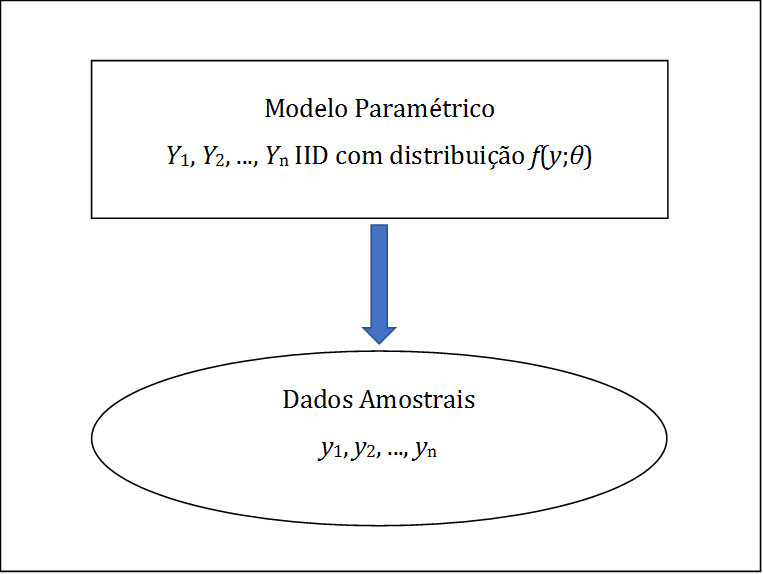
\includegraphics{Figuras/Figura2.1.png}
\caption{\label{fig:modclas}Representação esquemática da Modelagem Clássica}
\end{figure}

\begin{longtable}[]{@{}ll@{}}
\caption{\label{tab:modelclass} Representação esquemática da abordagem
1.}\tabularnewline
\toprule
\begin{minipage}[t]{0.29\columnwidth}\raggedright\strut
Dados Amostrais\strut
\end{minipage} & \begin{minipage}[t]{0.60\columnwidth}\raggedright\strut
\(Y_1=y_1,\ldots, Y_n=y_n\)\strut
\end{minipage}\tabularnewline
\begin{minipage}[t]{0.29\columnwidth}\raggedright\strut
Modelo Paramétrico/ Hipóteses\strut
\end{minipage} & \begin{minipage}[t]{0.60\columnwidth}\raggedright\strut
\(Y_1,\ldots,Y_n\) variáveis aleatórias IID com distribuição
\(f(y,\theta)\), onde \(\theta \in \Theta\)\strut
\end{minipage}\tabularnewline
\begin{minipage}[t]{0.29\columnwidth}\raggedright\strut
Objetivo\strut
\end{minipage} & \begin{minipage}[t]{0.60\columnwidth}\raggedright\strut
Inferir sobre \(\theta\) usando as observações \(y_1, \ldots,y_n\)\strut
\end{minipage}\tabularnewline
\bottomrule
\end{longtable}

Do ponto de vista matemático, o parâmetro \(\theta\) serve para indexar
os elementos da família de distribuições
\(\left\{f\left( y;\theta \right);\theta \in \Theta \right\}\). Na
prática, as questões relevantes da pesquisa são traduzidas em termos de
perguntas sobre o valor ou região a que pertence o parâmetro \(\theta\),
e a inferência sobre \(\theta\) a partir dos dados ajuda a responder
tais questões. Esta abordagem é útil em estudos analíticos tais como,
por exemplo, na investigação da natureza da associação entre variáveis
(modelos de regressão linear ou logística, modelos log-lineares, etc.).
Vários exemplos discutidos ao longo dos Capítulos \ref{modreg},
\ref{testqualajust} e \ref{testetab2} ilustram situações deste tipo. No
Capítulo \ref{estimacao-de-densidades} o foco vai ser a estimação não
paramétrica da forma da função \(f(y;\theta)\). Inferência sob modelos
do tipo descrito nesta seção forma o conteúdo de um curso introdutório
de inferência estatística. Mais detalhes podem ser consultados, por
exemplo, em \citep{Casella} e \citep{Marcos}.

\subsection{Abordagem 2 - Amostragem
Probabilística}\label{abordagem-2---amostragem-probabilistica}

A abordagem adotada pelos praticantes de amostragem (amostristas)
considera uma população finita \(U=\{1,\ldots ,N\}\), da qual é
selecionada uma amostra \(a=\left\{ i_{1},\ldots ,i_{n}\right\}\),
segundo um plano amostral caracterizado por \(p\left( a\right)\),
probabilidade de ser selecionada a amostra \(a\), suposta calculável
para todas as possíveis amostras. Os valores \(y_{1},\ldots ,y_{N}\) das
variáveis de interesse \(Y\) na população finita são considerados fixos,
porém desconhecidos. \textbar{}

A partir dos valores observados na amostra, denotados por
\(y_{i_1}, \ldots, y_{i_n}\), são feitas inferências a respeito de
funções dos valores populacionais, digamos
\(g\left( y_{1}, \ldots , y_{N}\right)\). Os valores de tais funções são
quantidades descritivas populacionais (QDPs), também denominadas
\texttt{parâmetros\ da\ população\ finita} pelos amostristas. Em geral,
o objetivo desta abordagem é fazer estudos descritivos utilizando
funções \(g\) particulares, tais como totais
\(g\left( y_{1}, \ldots , y_{N}\right) = \sum_{i=1}^{N} y_{i}\) , médias
\(g\left( y_{1}, \ldots , y_{N}\right) = N^{-1}\sum_{i=1}^{N} y_{i}\),
proporções, razões, etc. Uma descrição esquemática resumida dessa
abordagem é apresentada na Tabela \ref{tab:modelamo}, e uma
representação gráfica resumida na Figura \ref{fig:modamo}.

\begin{figure}
\centering
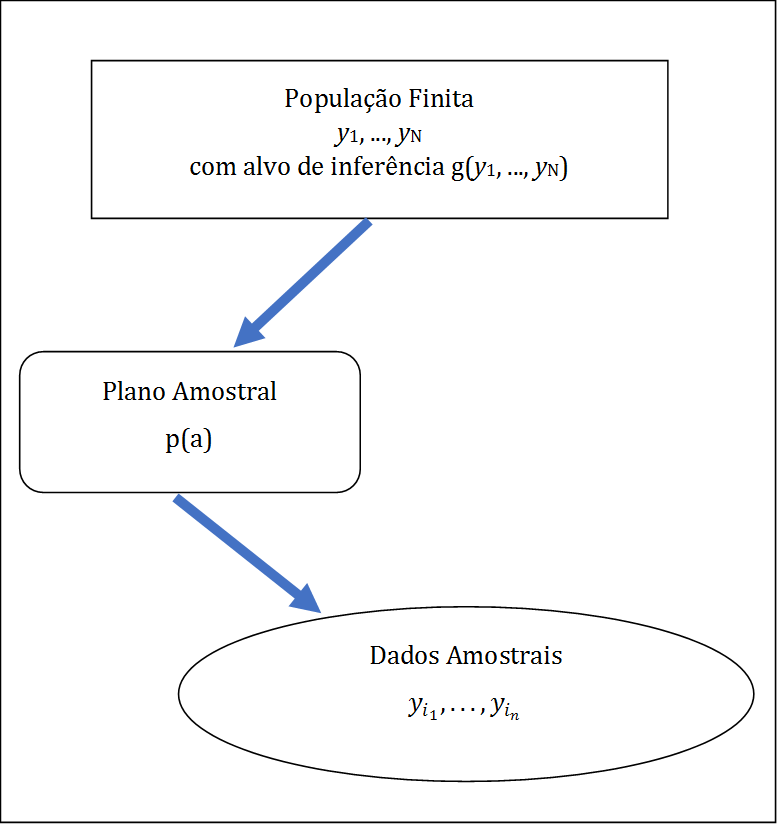
\includegraphics{Figuras/Figura2.2.png}
\caption{\label{fig:modamo}Amostragem Probabilística}
\end{figure}

\begin{longtable}[]{@{}ll@{}}
\caption{\label{tab:modelamo} Representação esquemática da abordagem
2.}\tabularnewline
\toprule
\begin{minipage}[t]{0.29\columnwidth}\raggedright\strut
Dados Amostrais\strut
\end{minipage} & \begin{minipage}[t]{0.60\columnwidth}\raggedright\strut
\(Y_1=y_{i_1}, \ldots, Y_n=y_{i_n}\)\strut
\end{minipage}\tabularnewline
\begin{minipage}[t]{0.29\columnwidth}\raggedright\strut
Hipóteses/Modelo Hipóteses\strut
\end{minipage} & \begin{minipage}[t]{0.60\columnwidth}\raggedright\strut
extraídos de \(y_1, \ldots , y_N\) segundo \(p(a)\)\strut
\end{minipage}\tabularnewline
\begin{minipage}[t]{0.29\columnwidth}\raggedright\strut
Objetivo\strut
\end{minipage} & \begin{minipage}[t]{0.60\columnwidth}\raggedright\strut
Inferir sobre funções \(g(y_1, \ldots , y_N)\) usando
\(y_{i_1}, \ldots, y_{i_n}\)\strut
\end{minipage}\tabularnewline
\bottomrule
\end{longtable}

\subsection{Discussão das Abordagens 1 e
2}\label{discussao-das-abordagens-1-e-2}

A primeira abordagem (Modelagem Clássica), nos termos descritos, foi
proposta como modelo para medidas na Física e Astronomia, onde em geral
o pesquisador tem relativo controle sobre os experimentos, e onde faz
sentido falar em replicação ou repetição do experimento. Neste contexto,
o conceito de aleatoriedade é geralmente introduzido para modelar os
erros (não controláveis) no processo de medição.

A segunda abordagem (Amostragem Probabilística) é utilizada
principalmente no contexto de estudos socioeconômicos, para levantamento
de dados por agências governamentais produtoras de informações
estatísticas. Nesta abordagem, a aleatoriedade é introduzida pelo
pesquisador no processo para obtenção dos dados, através do planejamento
amostral \(p(a)\) utilizado \citep{Neyman} e as distribuições das
estatísticas de interesse são derivadas a partir dessa
\texttt{distribuição\ de\ aleatorização}.

Os planos amostrais podem ser complexos, gerando observações com as
características i) a iv) do Capítulo \ref{introduc}. Os dados obtidos
são utilizados principalmente para descrição da população finita, sendo
calculadas estimativas de totais, médias, proporções, razões, etc. Sob
essa abordagem, os pontos i) a iv) do Capítulo \ref{introduc} são
devidamente considerados tanto na estimação de parâmetros descritivos
usuais, como também na estimação de variâncias dos estimadores.

A abordagem de amostragem probabilística é essencialmente
não-paramétrica, pois não supõe uma distribuição paramétrica particular
para as observações da amostra. Por outro lado, essa abordagem tem a
desvantagem de fazer inferências restritas à particular população finita
considerada.

Apesar dessa abordagem ter sido inicialmente concebida e aplicada para
problemas de inferência descritiva sobre populações finitas, é cada vez
mais comum, porém, a utilização de dados obtidos através de pesquisas
amostrais complexas para fins analíticos, com a aplicação de métodos de
análise desenvolvidos e apropriados para a \texttt{abordagem\ 1}.

Diante do exposto, podemos considerar algumas questões de interesse.

\begin{itemize}
\item
  É adequado aplicar métodos de análise da \texttt{abordagem\ 1},
  concebidos para observações IID, aos dados obtidos através de
  pesquisas amostrais complexas?
\item
  Em caso negativo, seria possível corrigir estes métodos, tornando-os
  aplicáveis para tratar dados amostrais complexos?
\item
  Ou seria mais adequado fazer uso analítico dos dados dentro da
  \texttt{abordagem\ 2}? E neste caso, como fazer isto, visto que nesta
  abordagem não é especificado um modelo para a distribuição das
  variáveis de pesquisa \texttt{na\ população}?
\end{itemize}

Além destas questões, também é de interesse a questão da robustez da
modelagem, traduzida nas seguintes perguntas.

\begin{itemize}
\tightlist
\item
  O que acontece quando o modelo adotado na \texttt{abordagem\ 1} não é
  verdadeiro?
\item
  Neste caso, qual a interpretação dos parâmetros na
  \texttt{abordagem\ 1}?
\item
  Ainda neste caso, as quantidades descritivas populacionais da
  \texttt{abordagem\ 2} poderiam ter alguma utilidade ou interpretação?
\end{itemize}

O objeto deste livro é exatamente discutir respostas para as questões
aqui enumeradas. Para isso, vamos considerar uma abordagem que propõe um
modelo parametrizado como na \texttt{abordagem\ 1} mas formulado para
descrever os dados da população, e não os da amostra. Além disso, essa
abordagem incorpora na análise os pontos i) a iii) do Capítulo
\ref{introduc} mediante aproveitamento da estrutura do planejamento
amostral, como feito habitualmente na \texttt{abordagem\ 2}. Essa
abordagem foi primeiro proposta em \citep{royall}, e é bem descrita, por
exemplo, em \citep{valliant}.

\subsection{Abordagem 3 - Modelagem de
Superpopulação}\label{modelsuperpop}

Nesta abordagem, os valores \(y_{1}, \ldots ,y_{N}\) das variáveis de
interesse \(Y\) na população finita são considerados observações ou
realizações dos vetores aleatórios \(Y_{1}, \ldots , Y_{N}\), supostos
IID com distribuição \(f(y;\theta)\), onde \(\theta \in \Theta\). Este
modelo é denominado \texttt{Modelo\ de\ Superpopulação}. Note que, em
contraste com o que se faz na \texttt{abordagem\ 1}, o modelo
probabilístico é aqui especificado para descrever o mecanismo aleatório
que gera \texttt{a\ população}, não \texttt{a\ amostra}. Na maioria das
aplicações práticas, a população de interesse, embora considerada finta,
jamais será observada por inteiro. Não obstante, ao formular o modelo
para descrever propriedades da população, nossas perguntas e respostas
descritas em termos de valores ou regiões para o parâmetro \(\theta\)
passam a se referir à população de interesse ou a populações similares,
quer existam ao mesmo tempo, quer se refiram a estados futuros (ou
passados) da mesma população. Vale realçar também que pesquisas por
amostragem ``consistem em selecionar parte de uma população para
observar, de modo que seja possível estimar alguma coisa sobre toda a
população'', conforme XXX Thompson (1992). XXX

Utilizando um plano amostral definido por \(p(a)\), obtemos os valores
das variáveis de pesquisa na amostra \(y_{i_1}, \ldots , y_{i_n}\). A
partir de \(y_{i_1}, \ldots , y_{i_n}\), em geral não considerados como
observações de vetores aleatórios IID, queremos fazer inferência sobre o
parâmetro \(\theta\), considerando os pontos i) a iii) do Capítulo 1.
Veja uma representação gráfica resumida desta abordagem na Figura
\ref{fig:modsup}.

\begin{figure}
\centering
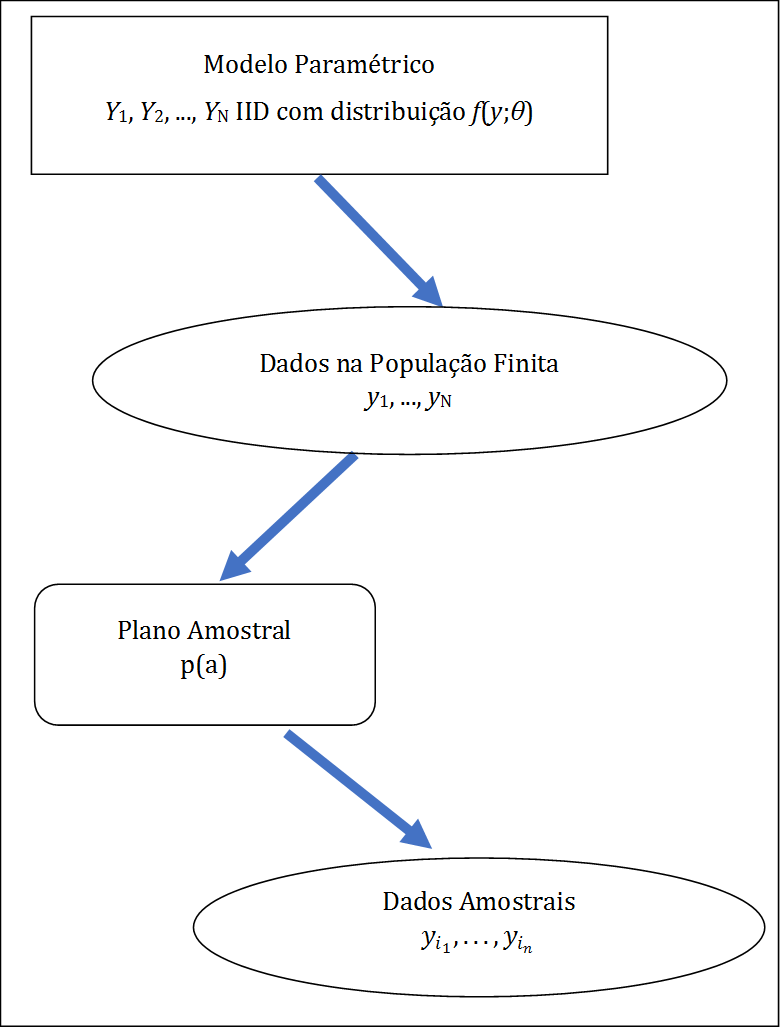
\includegraphics{Figuras/Figura2.3.png}
\caption{\label{fig:modsup}Modelagem de Superpopulação}
\end{figure}

Adotando o modelo de superpopulação e considerando métodos usuais
disponíveis na \texttt{abordagem\ 1}, podemos utilizar funções de
\(y_{1}, \ldots ,y_{N}\) , digamos \(g( y_{1}, \ldots , y_{N})\), para
fazer inferência sobre \(\theta\). Desta forma, definimos estatísticas
\(\left( y_{1},\ldots ,y_{N}\right)\) (no sentido da
\texttt{abordagem\ 1}) que são quantidades descritivas populacionais
(parâmetros populacionais no contexto da \texttt{abordagem\ 2}), que
passam a ser os novos parâmetros-alvo. O passo seguinte é utilizar
métodos disponíveis na \texttt{abordagem\ 2} para fazer inferência sobre
\(g\left( y_{1}, \ldots , y_{N}\right)\) baseada em
\(y_{i_1},\ldots ,y_{i_n}\). Note que não é possível basear a inferência
nos valores populacionais \(y_{1}, \ldots , y_{N}\), já que estes não
são conhecidos ou observados. Este último passo adiciona a informação
sobre o plano amostral utilizado, contida em \(p(a)\), à informação
estrutural contida no modelo
\(\left\{ f\left( y; \theta \right) ;\theta \in \Theta\right\}\). Uma
representação esquemática dessa abordagem é apresentada no Tabela
\ref{tab:modelsuperpop}.

\begin{longtable}[]{@{}ll@{}}
\caption{\label{tab:modelsuperpop} Representação esquemática da abordagem
3.}\tabularnewline
\toprule
\begin{minipage}[t]{0.29\columnwidth}\raggedright\strut
Dados Amostrais\strut
\end{minipage} & \begin{minipage}[t]{0.60\columnwidth}\raggedright\strut
\(Y_1=y_{i_1},\ldots,Y_n=y_{i_n}\)\strut
\end{minipage}\tabularnewline
\begin{minipage}[t]{0.29\columnwidth}\raggedright\strut
População e esquema de seleção\strut
\end{minipage} & \begin{minipage}[t]{0.60\columnwidth}\raggedright\strut
Extraídos de \(y_1,\dots,y_N\) segundo \(p(a)\)\strut
\end{minipage}\tabularnewline
\begin{minipage}[t]{0.29\columnwidth}\raggedright\strut
Modelo para poulação\strut
\end{minipage} & \begin{minipage}[t]{0.60\columnwidth}\raggedright\strut
\(Y_1, \dots, Y_N\) variáveis aleatórias IID com distribuição
\(f(y,\theta)\), onde \(\theta \in \Theta\)\strut
\end{minipage}\tabularnewline
\begin{minipage}[t]{0.29\columnwidth}\raggedright\strut
Parâmetro-alvo\strut
\end{minipage} & \begin{minipage}[t]{0.60\columnwidth}\raggedright\strut
associar
\(\theta \longleftrightarrow g\left(Y_{1}, \ldots , Y_{N}\right)\)\strut
\end{minipage}\tabularnewline
\begin{minipage}[t]{0.29\columnwidth}\raggedright\strut
Objetivo\strut
\end{minipage} & \begin{minipage}[t]{0.60\columnwidth}\raggedright\strut
Inferir sobre \(g\left( Y_{1}, \ldots , Y_{N}\right)\) partir de
\(y_{i_1},\ldots,y_{i_n}\) usando \(p\left( a\right)\)\strut
\end{minipage}\tabularnewline
\bottomrule
\end{longtable}

A descrição da abordagem adotada neste livro foi apresentada de maneira
propositadamente simplificada e vaga nesta seção, mas será aprofundada
ao longo do texto. Admitiremos que o leitor esteja familiarizado com a
\texttt{abordagem\ 1} e com as noções básicas da \texttt{abordagem\ 2}.
A título de recordação, serão apresentados no Capítulo \ref{planamo}
alguns resultados básicos da Teoria de Amostragem. A ênfase do texto,
porém, será na apresentação da \texttt{abordagem\ 3}, sendo para isto
apresentados os elementos indispensáveis das
\texttt{abordagens\ 1\ e\ 2}.

Ao construir e ajustar modelos a partir de dados de pesquisas amostrais
\texttt{complexas}, tais como as executadas pelo IBGE e outras
instituições similares, o usuário precisa incorporar as informações
sobre pesos e sobre a estrutura dos planos amostrais utilizados. Em
geral, ao publicar os resultados das pesquisas, os pesos são
considerados, sendo possível produzir estimativas pontuais
\texttt{corretas} utilizando os pacotes tradicionais. Por outro lado,
para construir intervalos de confiança e testar hipóteses sobre
parâmetros de modelos, seria preciso o conhecimento das estimativas de
variâncias e covariâncias das estimativas, obtidas levando em conta a
estrutura do plano amostral utilizado. Mesmo conhecendo o plano
amostral, geralmente não é simples incorporar pesos e plano amostral na
análise sem o uso de pacotes especializados, ou de rotinas específicas
já agora disponíveis em alguns dos pacotes mais comumente utilizados
(por exemplo, SAS, Stata, SPSS, ou R entre outros). Tais pacotes
especializados ou rotinas específicas utilizam, em geral, métodos
aproximados para estimar matrizes de covariância. Entre esses métodos,
destacam-se o de Máxima Pseudo-Verossimilhança, a Linearização, o método
do Conglomerado Primário, e métodos de reamostragem, que serão descritos
mais adiante.

Em outras palavras, o uso dos pacotes usuais para analisar dados
produzidos por pesquisas com planos amostrais complexos, tal como o uso
de muitos remédios, pode ter contra-indicações. Cabe ao usuário
\texttt{ler\ a\ bula} e identificar situações em que o uso de tais
pacotes pode ser inadequado, e buscar opções de rotinas específicas ou
de pacotes especializados capazes de incorporar adequadamente a
estrutura do plano amostral nas análises.

Ao longo deste livro faremos uso intensivo do pacote \texttt{survey}
disponível no R, mas o leitor encontrará funcionalidade semelhante em
vários outros pacotes. Nossa escolha se deveu a dois fatores principais:
primeiro ao fato do pacote R ser aberto, livre e gratuito, dispensando o
usuário de custos de licenciamento, bem como possibilitando aos
interessados o acesso ao código fonte e a capacidade de modificar as
rotinas de análise, caso necessário. O segundo fator é de natureza mais
técnica, porém transitória. No presente momento, o pacote
\texttt{survey} é a coleção de rotinas mais completa e genérica
existente para análise de dados amostrais complexos, dispondo de funções
capazes de ajustar os modelos usuais mas também de ajustar modelos não
convencionais mediante maximização de verossimilhanças especificadas
pelo usuário. Sabemos, entretanto, que muitos usuários habituados à
facilidade de uso de pacotes com interfaces gráficas do tipo
\texttt{aponte\ e\ clique} terão dificuldade adicional de adaptar-se à
linguagem de comandos utilizada pelo pacote R, mas acreditamos que os
benefícios do aprendizado desta nova ferramenta compensarão largamente
os custos adicionais do aprendizado.

O emprego de ferramentas de análise como o pacote \texttt{survey}
permitirá aos usuários focar sua atenção mais na seleção, análise e
interpretação dos modelos ajustados do que nas dificuldades técnicas
envolvidas nos cálculos correspondentes. E é com este espírito que
escrevemos este texto, que busca apresentar os métodos, ilustrando seu
uso com exemplos reais e orientando sobre o uso adequado das ferramentas
de modelagem e análise disponíveis no sistema R.

\section{Fontes de Variação}\label{fontes-de-variacao}

Esta seção estabelece um referencial para inferência em pesquisas
amostrais que será usado no restante deste texto. \citep{cassel} sugerem
que um referencial para inferência poderia usar três fontes de
aleatoriedade (incerteza, variação), incluindo:

\begin{enumerate}
\def\labelenumi{\arabic{enumi}.}
\item
  \texttt{Modelo\ de\ superpopulação}, que descreve o processo
  subjacente que, por hipótese, era as medidas verdadeiras de qualquer
  unidade da população considerada;
\item
  \texttt{Processo\ de\ medição}, que diz respeito aos instrumentos e
  métodos usados para obter as medidas de qualquer unidade da população;
\item
  \texttt{Planejamento\ amostral}, que estabelece o mecanismo pelo qual
  unidades da população são selecionadas para participar da amostra da
  pesquisa ou estudo.
\end{enumerate}

Uma quarta fonte de incerteza que precisa ser acrescentada às anteriores
é o

\begin{enumerate}
\def\labelenumi{\arabic{enumi}.}
\setcounter{enumi}{3}
\tightlist
\item
  \texttt{Mecanismo\ de\ resposta}, ou seja, o mecanismo que controla se
  valores de medições de unidades selecionadas para a amostra são
  obtidos / observados ou não.
\end{enumerate}

Para concentrar o foco nas questões de maior interesse deste texto, as
fontes (2) e (4) não serão consideradas no referencial adotado para a
maior parte dos capítulos. Para o tratamento das dificuldades causadas
por não resposta, a fonte (4) será considerada no capítulo onze. Assim
sendo, exceto onde explicitamente indicado, de agora em diante
admitiremos que não há \texttt{erros\ de\ medição}, implicando que os
valores observados de quaisquer variáveis de interesse serão
considerados valores corretos ou verdadeiros. Admitiremos ainda que há
\texttt{resposta\ completa}, implicando que os valores de quaisquer
variáveis de interesse estão disponíveis para todos os elementos da
amostra selecionada depois que a pesquisa foi realizada. Hipóteses
semelhantes são adotadas, por exemplo, em \citep{Mont87}.

Portanto, o referencial aqui adotado considera apenas duas fontes
alternativas de variação: o \texttt{Modelo\ de\ Superpopulação} (1) e o
\texttt{Plano\ Amostral} (3). Estas fontes alternativas de variação,
descritas nesta seção apenas de forma esquemática, são discutidas com
maiores detalhes a seguir.

A fonte de variação (1) será considerada porque usos analíticos das
pesquisas são amplamente discutidos neste texto, os quais só têm sentido
quando é especificado um modelo estocástico para o processo subjacente
que gera as medidas na população. A fonte de variação (3) será
considerada porque a atenção será focalizada na análise de dados obtidos
através de pesquisas amostrais complexas. Aqui a discussão se
restringirá a planos amostrais aleatorizados ou de amostragem
probabilística, não sendo considerados métodos intencionais ou outros
métodos não-aleatórios de seleção de amostras.

\section{Modelos de Superpopulação}\label{modelos-de-superpopulacao}

Seja \(\{1, ..., N\}\) um conjunto de rótulos que identificam
univocamente os \(N\) elementos distintos de uma população-alvo finita
\(U\). Sem perda de generalidade tomaremos \(U=\{1,...,N\}\). Uma
pesquisa cobrindo \(n\) elementos distintos numa amostra \(a\),
\(a=\{i_{1},...,i_{n}\}\subset U\), é realizada para medir os valores de
\(P\) variáveis de interesse da pesquisa, doravante denominadas
simplesmente \texttt{variáveis\ da\ pesquisa}.

Denotaremos por \(\mathbf{y}_i=(y_{i1},...,y_{iP})^{\prime }\) o vetor
\(P\times 1\) de valores das variáveis da pesquisa e por
\(\mathbf{x}_{i}=(x_{i1},...,x_{iQ})^{\prime }\) o vetor \(Q\times 1\)
de variáveis auxiliares da i-ésima unidade da população,
respectivamente, para \(i=1,...,N\). Aqui as variáveis auxiliares são
consideradas como variáveis contendo a informação requerida para o
planejamento amostral e a estimação a partir da amostra, como se
discutirá com mais detalhes adiante. Denote por \(\mathbf{y}_{U}\) a
matriz \(N \times P\) formada empilhando os vetores transpostos das
observações das variáveis de pesquisa correspondentes a todas as
unidades da população, e por \(\mathbf{Y}_{U}\) a correspondente matriz
de vetores aleatórios geradores das observações na população.

Quando se supõe que \(\mathbf{y}_1 ,\ldots, \mathbf{y}_N\) são a
realização conjunta de vetores aleatórios
\(\mathbf{Y}_1 ,\ldots, \mathbf{Y}_N\), a distribuição conjunta de
probabilidade de \(\mathbf{Y}_1 ,\ldots, \mathbf{Y}_N\) é um modelo
(marginal) de superpopulação, que doravante denotaremos simplesmente por
\(f(\mathbf{y}_U;\theta)\), ou de forma abreviada, por \(M\) para
indicar que se trata do \texttt{modelo\ marginal\ de\ superpopulação}.
Esperanças e variâncias definidas com respeito à distribuição do modelo
marginal \(M\) serão denotadas \(E_M\) e \(V_M\) respectivamente.

Analogamente, \(\mathbf{x}_1 ,\ldots, \mathbf{x}_N\) pode ser
considerada uma realização conjunta de vetores aleatórios
\(\mathbf{X}_1 ,\ldots, \mathbf{X}_N\). As matrizes \(N \times Q\)
formadas empilhando os vetores transpostos das observações das variáveis
auxiliares correspondentes a todas as unidades da população,
\(\mathbf{x}_{U}\), e a correspondente matriz \(\mathbf{X}_{U}\) de
vetores aleatórios geradores das variáveis auxiliares na população são
definidas de forma análoga às matrizes \(\mathbf{y}_{U}\) e
\(\mathbf{Y}_{U}\).

O referencial aqui adotado permite a especificação da distribuição
conjunta combinada das variáveis da pesquisa e das variáveis auxiliares.
Representamos por \(f( \mathbf{y}_U , \mathbf{x}_U ; \mathbf{\eta} )\) a
função de densidade de probabilidade de
\(( \mathbf{Y}_U , \mathbf{X}_U )\), onde \(\mathbf{\eta}\) é um vetor
de parâmetros.

Um tipo importante de modelo de superpopulação é obtido quando os
vetores aleatórios correspondentes às observações de unidades diferentes
da população são supostos independentes e identicamente distribuídos
(IID). Neste caso, o modelo de superpopulação pode ser escrito como:

\begin{eqnarray}
f \left( \mathbf{y}_U , \mathbf{x}_U ; \mathbf{\eta} \right) 
&=&\prod_{i\in U} f\left(\mathbf{y}_i , \mathbf{x}_i ; \mathbf{\eta} \right) \label{eq:ref1} \\
&=&\prod_{i\in U} f\left( \mathbf{y}_i \mathbf{|x}_i ; \mathbf{\lambda} \right) 
f\left( \mathbf{x}_i ; \mathbf{\phi} \right) \label{eq:ref2}
\end{eqnarray}

onde~\(\mathbf{\lambda}\) e \(\mathbf{\phi}\) são vetores de parâmetros.

Sob \eqref{eq:ref2}, o modelo marginal correspondente das variáveis da
pesquisa seria obtido integrando nas variáveis auxiliares:

\begin{equation}
f(\mathbf{y}_U ; \mathbf{\theta}) = f(\mathbf{y}_1 ,\ldots ,\mathbf{y}_N ; \mathbf{\theta}) = \prod_{i\in U} \int f\left( \mathbf{y}_i \mathbf{|x}_i ; \mathbf{\lambda} \right) f\left( \mathbf{x}_i ; \mathbf{\phi} \right) \mathbf{dx}_i = \prod_{i\in U} f\left( \mathbf{y}_i ; \mathbf{\theta} \right) \label{eq:ref3}
\end{equation}

onde
\(f\left( \mathbf{y}_i ; \mathbf{\theta} \right) = \int f\left( \mathbf{y}_i | \mathbf{x}_i ; \mathbf{\lambda} \right) f\left( \mathbf{x}_i ; \mathbf{\phi} \right) \mathbf{dx}_i\)
e
\(\mathbf{\theta =} h\left( \mathbf{\lambda} , \mathbf{\phi} \right)\).

Outro tipo especial de modelo de superpopulação é o modelo de população
fixa, que supõe que os valores numa população finita são fixos mas
desconhecidos. Este modelo pode ser descrito por:

\begin{equation}
P\left[ \left( \mathbf{Y}_U , \mathbf{X}_U \right) = \left( \mathbf{y}_U , \mathbf{x}_U \right) \right] = 1 \label{eq:ref4}
\end{equation}

ou seja, uma distribuição degenerada é especificada para
\(\left(\mathbf{Y}_U , \mathbf{X}_U \right)\).

Este modelo foi considerado em \citep{cassel}, que o chamaram de
\texttt{abordagem\ de\ população\ fixa} e afirmaram ser esta a abordagem
subjacente ao desenvolvimento da teoria de amostragem encontrada nos
livros clássicos tais como \citep{cochran} e outros. Aqui esta abordagem
é chamada de \texttt{abordagem\ baseada\ no\ planejamento\ amostral} ou
\texttt{abordagem\ de\ aleatorização}, pois neste caso a única fonte de
variação (aleatoriedade) é proveniente do planejamento amostral. Em
geral, a distribuição conjunta de
\(\left( \mathbf{Y}_U , \mathbf{X}_U \right)\) não precisa ser
degenerada como em \eqref{eq:ref4}, embora o referencial aqui adotado seja
suficientemente geral para permitir considerar esta possibilidade.

Se todas as unidades da população fossem pesquisadas (ou seja, se fosse
executado um censo), os dados observados seriam
\((\mathbf{y}_1 , \mathbf{x}_1) ,\ldots, (\mathbf{y}_N , \mathbf{x}_N)\).
Sob a hipótese de resposta completa, a única fonte de incerteza seria
devida ao fato de que
\((\mathbf{y}_1 , \mathbf{x}_1) ,\ldots, (\mathbf{y}_N , \mathbf{x}_N)\)
é uma realização de
\(\left( \mathbf{Y}_1 , \mathbf{X}_1 \right) ,\ldots, \left( \mathbf{Y}_N , \mathbf{X}_N \right)\).
Os dados observados poderiam então ser usados para fazer inferências
sobre \(\mathbf{\eta}, \mathbf{\phi},\mathbf{\lambda}\) ou
\(\mathbf{\theta}\) usando procedimentos padrões.

Inferência sobre quaisquer dos parâmetros
\(\mathbf{\eta},\mathbf{\phi},\mathbf{\lambda}\) ou \(\mathbf{\theta}\)
do modelo de superpopulação é chamada \texttt{inferência\ analítica}.
Este tipo de inferência só faz sentido quando o modelo de superpopulação
não é degenerado como em \eqref{eq:ref4}. Usualmente seu objetivo é
explicar a relação entre variáveis não apenas para a população finita
sob análise, mas também para outras populações que poderiam ter sido
geradas pelo modelo de superpopulação adotado. Vários exemplos de
inferência analítica serão discutidos ao longo deste livro.

Se o objetivo da inferência é estimar quantidades que fazem sentido
somente para a população finita sob análise, tais como funções
\(g\left( \mathbf{y}_1 ,\ldots, \mathbf{y}_N \right)\) dos valores das
variáveis da pesquisa, o modelo de superpopulação não é estritamente
necessário, embora possa ser útil. Inferência para tais quantidades,
chamadas parâmetros da população finita ou quantidades descritivas
populacionais (QDPs), é chamada \texttt{inferência\ descritiva}.

\section{Planejamento Amostral}\label{planamo}

Embora censos sejam algumas vezes realizados para coletar dados sobre
certas populações, a vasta maioria das pesquisas realizadas é de
pesquisas amostrais, nas quais apenas uma amostra de elementos da
população (usualmente uma pequena parte) é investigada. Neste caso, os
dados disponíveis incluem:

\begin{enumerate}
\def\labelenumi{\arabic{enumi}.}
\item
  O conjunto de rótulos \(a=\left\{ i_1 , \ldots, i_n \right\}\) dos
  distintos elementos na amostra, onde \(n\)
  \(\left( 1 \leq n \leq N \right)\) é o número de elementos na amostra
  \(a\), chamado tamanho da amostra;
\item
  Os valores na amostra das variáveis da pesquisa
  \(\mathbf{y}_{i_1} ,\ldots, \mathbf{y}_{i_n}\);
\item
  Os valores das variáveis auxiliares na população
  \(\mathbf{x}_1 ,\ldots, \mathbf{x}_N\), quando a informação auxiliar é
  dita \texttt{completa}; alternativamente, os valores das variáveis
  auxiliares na amostra \(\mathbf{x}_{i_1} ,\ldots, \mathbf{x}_{i_n}\),
  mais os totais ou médias destas variáveis na população, quando a
  informação auxiliar é dita \texttt{parcial}.
\end{enumerate}

O mecanismo usado para selecionar a amostra \(a\) da população finita
\(U\) é chamado plano amostral. Uma forma de caracterizá-lo é através da
função \(p\left( .\right)\), onde \(p(a)\) dá a probabilidade de
selecionar a amostra \(a\) no conjunto \(A\) de todas as amostras
possíveis. Só mecanismos amostrais envolvendo alguma forma de seleção
probabilística bem definida serão aqui considerados, e portanto supõe-se
que \(0 \leq p(a) \leq 1 \; \forall a \in A\) e
\(\sum_{a \in A} p(a)=1\).

Esta caracterização do plano amostral \(p(a)\) é bem geral, permitindo
que o mecanismo de seleção amostral dependa dos valores das variáveis
auxiliares \(\mathbf{x}_1 ,\ldots, \mathbf{x}_N\) bem como dos valores
das variáveis da pesquisa na população
\(\mathbf{y}_1 ,\ldots, \mathbf{y}_N\) (amostragem \texttt{informativa},
veja Seção \ref{inform}. Uma notação mais explícita para indicar esta
possibilidade envolveria escrever \(p(a)\) como
\(p\left[ a | (\mathbf{y}_U , \mathbf{x}_U ) \right]\). Tal notação será
evitada por razões de simplicidade.

Denotamos por \(I(B)\) a função indicadora que assume o valor 1 quando o
evento \(B\) ocorre e 0 caso contrário. Seja
\(\mathbf{\Delta}_a = \left[ I(1 \in a) ,\ldots, I(N \in a)\right]^{\prime}\)
um vetor aleatório de indicadores dos elementos incluídos na amostra
\(a\). Então o plano amostral pode ser alternativamente caracterizado
pela distribuição de probabilidade de \(\mathbf{\Delta }_a\) denotada
por
\(f\left[ \mathbf{\delta }_a | \left(\mathbf{y}_U , \mathbf{x}_U \right) \right]\),
onde \(\mathbf{\delta }_a\) é qualquer realização particular de
\(\mathbf{\Delta }_a\) tal que
\({\mathbf{\delta}_a}^{\prime} \mathbf{1}_N = n\), e \(\mathbf{1}_N\) é
o vetor unitário de dimensão \(N\).

Notação adicional necessária nas seções posteriores será agora
introduzida. Denotamos por \(\pi_i\) a probabilidade de inclusão da
unidade \(i\) na amostra \(a\), isto é,

\begin{equation}
\pi_i = Pr\left( i \in a \right) = \sum_{a \ni i} p(a)  \label{eq:ref5}
\end{equation}

e denotamos por \(\pi_{ij}\) a probabilidade de inclusão conjunta na
amostra das unidades \(i\) e \(j\), dada por

\begin{equation}
\pi_{ij} = Pr \left( i \in a , j \in a \right) = \sum_{a \ni i,j} p(a) \label{eq:ref6}
\end{equation}

para todo \(i \neq j \in U\), e seja \(\pi_{ii} = \pi_{i}\)
\(\forall i \in U.\)

Uma hipótese básica assumida com relação aos planos amostrais aqui
considerados é que \(\pi_i > 0\) e \(\pi_{ij} > 0\)
\(\forall i,j \in U.\) A hipótese de \(\pi_{ij}\) ser positiva é adotada
para simplificar a apresentação de expressões para estimadores de
variância dos estimadores dos parâmetros de interesse. Contudo, esta não
é uma hipótese crucial, pois há planos amostrais que não a satisfazem e
para os quais estão disponíveis aproximações e estimadores satisfatórios
das variâncias dos estimadores de totais e de médias.

\section{Planos Amostrais Informativos e Ignoráveis}\label{inform}

Ao fazer inferência usando dados de pesquisas amostrais precisamos
distinguir duas situações que requerem tratamento diferenciado. Uma
dessas situações ocorre quando o plano amostral empregado para coletar
os dados é \texttt{informativo}, isto é, quando o mecanismo de seleção
das unidades amostrais pode depender dos valores das variáveis de
pesquisa. Um exemplo típico desta situação é o dos
\texttt{estudos\ de\ caso-controle}, em que a amostra é selecionada de
tal forma que há \texttt{casos} (unidades com determinada condição) e
\texttt{controles} (unidades sem essa condição), sendo de interesse a
modelagem do indicador de presença ou ausência da condição em função de
variáveis preditoras, e sendo esse indicador uma das variáveis de
pesquisa, que é considerada no mecanismo de seleção da amostra. Os
métodos que discutiremos ao longo deste livro não são adequados, em
geral, para esse tipo de situação, e portanto uma hipótese fundamental
adotada ao longo deste texto é que os planos amostrais considerados são
\texttt{não-informativos}, isto é, não podem depender diretamente dos
valores das variáveis da pesquisa. Logo eles satisfazem:

\begin{equation}
f\left[ \mathbf{\delta }_a | \left( \mathbf{y}_U , \mathbf{x}_U \right)
\right] = f\left( \mathbf{\delta }_a | \mathbf{x}_U \right) . \label{eq:ref7}
\end{equation}

Entre os planos amostrais \texttt{não-informativos}, precisamos ainda
distinguir duas outras situações de interesse. Quando o plano amostral é
Amostragem Aleatória Simples Com Reposição (AASC), o modelo adotado para
a amostra é o mesmo que o modelo adotado para a população antes da
amostragem. Quando isto ocorre, o plano amostral é dito
\texttt{ignorável}, porque a inferência baseada na amostra utilizando a
abordagem clássica descrita em \ref{classic} pode prosseguir sem
problemas. Entretanto, esquemas amostrais desse tipo são raramente
empregados na prática, por razões de eficiência e custo. Em vez disso,
são geralmente empregados planos amostrais envolvendo estratificação,
conglomeração e probabilidades desiguais de seleção
(\texttt{amostragem\ complexa}).

Com amostragem complexa, porém, os modelos para a população e a amostra
podem ser muito diferentes (plano amostral \texttt{não-ignorável}),
mesmo que o mecanismo de seleção não dependa das variáveis de pesquisa,
mas somente das variáveis auxiliares. Neste caso, ignorar o plano
amostral pode viciar a inferência. Veja o Exemplo \ref{exm:nonigno}
adiante.

A definição precisa de ignorabilidade e as condições sob as quais um
plano amostral é ignorável para inferência são bastante discutidas na
literatura - veja por exemplo \citep{Sugden84} ou os Capítulos 1 e 2 de
\citep{CHSK2003}. Porém testar a ignorabilidade do plano amostral é
muitas vezes complicado. Em caso de dificuldade, o uso de pesos tem
papel fundamental.

Uma forma simples de lidar com os efeitos do plano amostral na estimação
pontual de quantidades descritivas populacionais de interesse é
incorporar pesos adequados na análise, como se verá no Capítulo
\ref{capplanamo}. Essa forma porém, não resolve por si só o problema de
estimação da precisão das estimativas pontuais, nem mesmo o caso da
estimação pontual de parâmetros em modelos de superpopulação, o que vai
requerer métodos específicos discutidos no Capítulo \ref{ajmodpar}.

Como incluir os pesos para proteger contra planos amostrais
\texttt{não-ignoráveis} e a possibilidade de má especificação do modelo?
Uma ideia é modificar os estimadores dos parâmetros de modo que sejam
consistentes (em termos da distribuição de aleatorização) para
quantidades descritivas da população finita da qual a amostra foi
extraída, que por sua vez seriam boas aproximações para os parâmetros
dos modelos de interesse. Afirmações probabilísticas são então feitas
com respeito à distribuição de aleatorização das estatísticas amostrais
\(p\) ou com respeito à distribuição mista ou combinada \(Mp\).

A seguir apresentamos um exemplo com a finalidade de ilustrar uma
situação de plano amostral não-ignorável.

\BeginKnitrBlock{example}
\protect\hypertarget{exm:nonigno}{}{\label{exm:nonigno} }Efeito da
amostragem estratificada simples com alocação desproporcional
\EndKnitrBlock{example}

Considere \(N\) observações de uma população finita \(U\) onde são
consideradas de interesse duas variáveis binárias \((x_i ; y_i )\).
Suponha que na população os vetores aleatórios \((X_i ; Y_i )\) são
independentes e identicamente distribuídos com distribuição de
probabilidades conjunta dada por:

\begin{longtable}[]{@{}cccc@{}}
\caption{\label{tab:Tab24} Distribuição de probabilidades conjunta na
população \(Pr( Y_i = y ; X_i = x )\).}\tabularnewline
\toprule
& & \(y\) &\tabularnewline
\midrule
\endfirsthead
\toprule
& & \(y\) &\tabularnewline
\midrule
\endhead
\(x\) & 0 & 1 & Total\tabularnewline
0 & \(\eta_{00}\) & \(\eta_{01}\) & \(\eta_{0+}\)\tabularnewline
1 & \(\eta_{10}\) & \(\eta_{11}\) & \(\eta_{1+}\)\tabularnewline
Total & \(\eta_{+0}\) & \(\eta_{+1}\) & 1\tabularnewline
\bottomrule
\end{longtable}

que também pode ser representada por:

\begin{eqnarray}
 f_U (x ; y) &=& Pr( X = x ; Y = y )\\
             & =& \eta_{00}^{(1-x)(1-y)} \times \eta_{01}^{(1-x)y} \times \eta_{10}^{x(1-y)} (1 - \eta_{00} - \eta_{01} - \eta_{10})^{xy} \nonumber
\end{eqnarray}

onde a designação \(f_U\) é utilizada para denotar a distribuição
\texttt{na\ população}.

Note agora que a distribuição marginal da variável \(Y\)
\texttt{na\ população} é Bernoulli com parâmetro
\(1 - \eta_{00} - \eta_{10}\), ou alternativamente:

\begin{equation}
 f_U (y) = Pr( Y = y ) = (\eta_{00} + \eta_{10})^{(1-y)} \times (1 - \eta_{00} - \eta_{10})^y
\end{equation}

De forma análoga, a distribuição marginal da variável \(X\)
\texttt{na\ população} também é Bernoulli, mas com parâmetro
\(1 - \eta_{00} - \eta_{01}\), ou alternativamente:

\begin{equation}
 f_U (x) = Pr( X = x ) = (\eta_{00} + \eta_{01})^{(1-x)} \times (1 - \eta_{00} - \eta_{01})^x
\end{equation}

Seja \(N_{xy}\) o número de unidades na população com a combinação de
valores observados \((x;y)\), onde \(x\) e \(y\) tomam valores em
\(\Omega = \{ 0 ; 1 \}\). É fácil notar então que o vetor de contagens
populacionais
\(\mathbf{N} = ( N_{00}, N_{01}, N_{10}, N_{11} )^{\prime}\) tem
distribuição Multinomial com parâmetros \(N\) e
\(\mathbf{\eta} = (\eta_{00} , \eta_{01} , \eta_{10} , 1 - \eta_{00} - \eta_{01} - \eta_{10} )^{\prime}\).

Após observada uma realização do modelo que dê origem a uma população,
como seria o caso da realização de um censo na população, a proporção de
valores de \(y\) iguais a 1 observada no censo seria dada por
\((N_{+1} / N = 1 - (N_{00} - N_{10})/N\). E a proporção de valores de
\(x\) iguais a 1 na população seria igual a
\((N_{1+} / N = 1 - (N_{00} - N_{01})/N\).

Agora suponha que uma amostra estratificada simples
\texttt{com\ reposição} de tamanho \(n\) inteiro e par seja selecionada
da população, onde os estratos são definidos com base nos valores da
variável \(x\), e onde a alocação da amostra nos estratos é dada por
\(n_0 = n_1 = n/2\), sendo \(n_x\) o tamanho da amostra no estrato
correspondente ao valor \(x\) usado como índice. Esta alocação é dita
\texttt{alocação\ igual}, pois o tamanho total da amostra é repartido em
partes iguais entre os estratos definidos para seleção, e no caso, há
apenas dois estratos. A alocação desta amostra será desproporcional
exceto no caso em que \(N_{0+} = N_{1+}\).

Nosso interesse aqui é ilustrar o efeito que uma alocação
desproporcional pode causar na análise dos dados amostrais, caso não
sejam levadas em conta na análise informações relevantes sobre a
estrutura do plano amostral. Para isto, vamos precisar obter a
distribuição amostral da variável de interesse \(Y\). Isto pode ser
feito em dois passos. Primeiro, note que a distribuição condicional de
\(Y\) dado \(X\) na população é dada por:

\begin{longtable}[]{@{}cccc@{}}
\caption{\label{tab:Tab25} Distribuição de probabilidades condicional de
\(y\) dado \(x\) na população -
\(Pr( Y_i = y | X_i = x )\).}\tabularnewline
\toprule
& & \(y\) &\tabularnewline
\midrule
\endfirsthead
\toprule
& & \(y\) &\tabularnewline
\midrule
\endhead
\(x\) & 0 & 1 & Total\tabularnewline
0 & \(\eta_{00}/\eta_{0+}\) & \(\eta_{01}/\eta_{0+}\) & 1\tabularnewline
1 & \(\eta_{10}/\eta_{1+}\) & \(\eta_{11}/\eta_{1+}\) & 1\tabularnewline
\bottomrule
\end{longtable}

ou, alternativamente

\begin{eqnarray}
 f_U (y | x) &=& Pr( Y = y | X = x )\\
             & =& (1-x) \times \frac{\eta_{00}^{(1-y)} \eta_{01}^y}   {\eta_{00}+\eta_{01}} + x \times \frac{\eta_{10}^{(1-y)} (1 - \eta_{00} - \eta_{01} - \eta_{10})^y} {1 - \eta_{00} - \eta_{01}}\nonumber
\end{eqnarray}

Dado o plano amostral acima descrito, a distribuição marginal de \(X\)
\texttt{na\ amostra} é Bernoulli com parâmetro \(1/2\). Isto segue
devido ao fato de que a amostra foi alocada igualmente com base nos
valores de \(x\) na população, e portanto, sempre teremos metade da
amostra com valores de \(x\) iguais a \(0\) e metade com valores iguais
a \(1\). Isto pode ser representado como:

\begin{equation}
 f_a (x) = Pr( X_i = x | i \in a ) = 1 / 2,\; \forall x \in \Omega \mbox{ e } \forall i \in U
\end{equation}

onde a designação \(f_a\) é utilizada para denotar a distribuição
\texttt{na\ amostra}.

Podemos usar a informação sobre a distribuição condicional de \(Y\) dado
\(X\) na população e a informação sobre a distribuição marginal de \(X\)
na amostra para obter a distribuição marginal de \(Y\) na amostra, que é
dada por:

\begin{eqnarray}
 f_a (y) &= &Pr( Y_i = y | i \in a )\\ 
&=& \sum _{x = 0} ^{1} Pr( X_i = x ; Y_i = y | i \in a) \nonumber \\ 
&=& \sum _{x = 0} ^{1} Pr[ Y_i = y | (X_i = x) e (i \in a)] \times Pr( X_i = x | i \in a) \nonumber\\ 
&=& \sum _{x = 0} ^{1} Pr( Y_i = y | X_i = x) \times f_a (x) \nonumber \\ 
&=& \sum _{x = 0} ^{1} f_U ( y | x) f_a (x) \nonumber \\ 
&=& \frac{1}{2} \times \left[ \frac{\eta_{00}^{(1-y)} \eta_{01}^y} {\eta_{00}+\eta_{01}}+ \frac{\eta_{10}^{(1-y)} (1 - \eta_{00} - \eta_{01} - \eta_{10})^y} {1 - \eta_{00} - \eta_{01}} \right]\nonumber
\end{eqnarray}

Isto mostra que a distribuição marginal de \(Y\) na amostra é diferente
da distribuição marginal de \(Y\) na população, mesmo quando o plano
amostral é especialmente simples e utiliza amostragem aleatória simples
com reposição dentro de cada estrato definido pela variável \(X\). Isto
ocorre devido à alocação desproporcional da amostra, apesar de a
distribuição condicional de \(Y\) dado \(X\) na população ser a mesma e
que a distribuição condicional de \(Y\) dado \(X\) na amostra.

Um exemplo numérico facilita a compreensão. Se a distribuição conjunta
de \(X\) e \(Y\) na população é dada por:

\begin{longtable}[]{@{}cclc@{}}
\caption{\label{tab:Tab26} Distribuição de probabilidades conjunta na
população \(f_U( x ; y )\).}\tabularnewline
\toprule
& \(y\) & &\tabularnewline
\midrule
\endfirsthead
\toprule
& \(y\) & &\tabularnewline
\midrule
\endhead
\(x\) & 0 & 1 & Total\tabularnewline
0 & 0,7 & 0,1 & 0,8\tabularnewline
1 & 0,1 & 0,1 & 0,2\tabularnewline
Total & 0,8 & 0,2 & 1\tabularnewline
\bottomrule
\end{longtable}

segue-se que a distribuição condicional de \(Y\) dado \(X\) na população
(e também na amostra) é dada por

\begin{longtable}[]{@{}cccc@{}}
\caption{\label{tab:Tab27} Distribuição de probabilidades condicional de
\(Y\) dado \(X\) na população - \(f_U( y | x )\).}\tabularnewline
\toprule
& \(y\) & &\tabularnewline
\midrule
\endfirsthead
\toprule
& \(y\) & &\tabularnewline
\midrule
\endhead
\(x\) & 0 & 1 & Total\tabularnewline
0 & 0,875 & 0,125 & 1\tabularnewline
1 & 0,500 & 0,500 & 1\tabularnewline
\bottomrule
\end{longtable}

e que a distribuição marginal de \(Y\) na população e na amostra são
dadas por

\begin{longtable}[]{@{}ccc@{}}
\caption{\label{tab:Tab28} Distribuição de probabilidades marginal de \(Y\)
na população - \(f_U( y )\).}\tabularnewline
\toprule
\(y\) & 0 & 1\tabularnewline
\midrule
\endfirsthead
\toprule
\(y\) & 0 & 1\tabularnewline
\midrule
\endhead
\(f_U(y)\) & 0,8000 & 0,2000\tabularnewline
\(f_a(y)\) & 0,6875 & 0,3125\tabularnewline
\bottomrule
\end{longtable}

Assim, inferência sobre a distribuição de \(Y\) \texttt{na\ população}
levada a cabo a partir dos dados da amostra observada sem considerar a
estrutura do plano amostral seria equivocada, pois a alocação igual da
amostra nos estratos levaria à observação de uma proporção maior de
valores de \(X\) iguais a 1 na amostra (1/2) do que a correspondente
proporção existente na população (1/5). Em conseqüência, a proporção de
valores de \(Y\) iguais a 1 na amostra (0.3125) seria 56\% maior que a
correspondente proporção na população (0.2).

Este exemplo é propositalmente simples, envolve apenas duas variáveis
com distribuição Bernoulli, mas ilustra bem como a amostragem pode
modificar distribuições de variáveis da amostra em relação à
correspondente distribuição na população.

Caso a inferência requerida fosse sobre parâmetros da distribuição
condicional de \(Y\) dado \(X\), a amostragem seria ignorável, isto é,
\(f_a ( y | x) = f_U (y | x)\). Assim, fica evidenciado também que a
noção de que o plano amostral pode ser ignorado depende da inferência
desejada. No nosso exemplo, o plano amostral é ignorável para inferência
sobre a distribuição condicional de \(Y\) dado \(X\), mas não é
ignorável para inferência sobre a distribuição marginal de \(Y\).

\chapter{Estimação Baseada no Plano Amostral}\label{capplanamo}

\section{Estimação de Totais}\label{estimatotais}

Devido a sua importância para os desenvolvimentos teóricos em vários dos
capítulos subsequentes, alguns resultados básicos relativos à estimação
de totais da população finita numa abordagem baseada no plano amostral
serão reproduzidos nesta seção. A referência básica usada foi a Seção
2.8 de \citep{SSW92}.

Consideremos o problema de estimar o vetor
\(\mathbf{Y}=\sum_{i \in U}\mathbf{y}_i\) de totais das \(P\) variáveis
da pesquisa na população, a partir de uma amostra observada \(a\).
Naturalmente, qualquer estimador viável do total \(\mathbf{Y}\) só pode
depender dos valores das variáveis de pesquisa observados na amostra,
contidos em \(\mathbf{y}_{i_{1}}, \ldots , \mathbf{y}_{i_{n}}\), mas não
dos valores dessas variáveis para os elementos não pesquisados.

Um estimador usual baseado no plano amostral para o total \(\mathbf{Y}\)
é o estimador de Horvitz-Thompson, também chamado \emph{estimador}
\(\pi\) \emph{-ponderado} (veja p.42 de \citep{SSW92}), dado por:

\begin{equation}
\hat{\mathbf{Y}}_\pi = \sum_{i \in a} \mathbf{y}_i / \pi_{i} . \label{eq:estpa1}
\end{equation}

Na abordagem baseada no planejamento amostral, as propriedades de uma
estatística ou estimador são avaliadas com respeito à distribuição de
aleatorização. Denotemos por \(E_p(.)\) e \(V_p(.)\) os operadores de
esperança e variância referentes à distribuição de probabilidades
\(p(a)\) induzida pelo planejamento amostral, que chamaremos daqui por
diante de \texttt{esperança\ \ de\ aleatorização} e
\texttt{variância\ de\ aleatorização}.

O estimador \(\pi\)-ponderado \(\mathbf{\hat{Y}}_{\pi}\) é não-viciado
para o total \(\mathbf{Y}\) com respeito à distribuição de
aleatorização, isto é

\[
E_p \left( \mathbf{\hat{Y}}_{\pi} \right) = \mathbf{Y} . 
\] Além disto, sua variância de aleatorização é dada por

\begin{equation}
V_p \left( \mathbf{\hat{Y}}_{\pi} \right) = \sum_{ i \in U} \, \sum_{j \in U} \left( \pi _{ij} - \pi_i \pi_j \right) \frac{ \mathbf{y}_i} {\pi_i} \frac{\mathbf{y}_j ^{\prime} } {\pi_j} \; .  \label{eq:estpa2}
\end{equation}

Uma expressão alternativa da variância de aleatorização de
\(\mathbf{\hat{Y}}_{\pi}\) , válida quando o plano amostral é de tamanho
fixo, é dada por

\begin{equation}
V_p \left( \mathbf{\hat{Y}}_{\pi} \right) = -\frac{1}{2} \sum_{i \in U} \, \sum_{j \in U} \left( \pi_{ij} - \pi_i \pi_j \right) \left( \frac{\mathbf{y}_i} {\pi_i} - \frac{\mathbf{y}_j} {\pi_j} \right) \left( \frac{\mathbf{y}_i} {\pi_i} - \frac{\mathbf{y}_j} {\pi_j} \right) ^{^{\prime}}.  \label{eq:estpa3}
\end{equation}

Note que na expressão \eqref{eq:estpa3} os termos onde \(i=j\) não
contribuem para a soma. Dois estimadores são usualmente recomendados
para estimar a variância de aleatorização de \(\mathbf{\hat{Y}}_{\pi}\).
O primeiro é motivado pela expressão \eqref{eq:estpa2} e é dado por

\begin{equation}
\hat{V}_p \left( \mathbf{\hat{Y}}_{\pi} \right) = \sum_{i \in a} \, \sum_{j \in a} \frac{\pi_{ij} - \pi_i \pi_j} {\pi_{ij}} \frac{\mathbf{y}_i} {\pi_i} \frac{\mathbf{y}_j^{^{\prime}}} {\pi_j} \mbox{.}  \label{eq:estpa4}
\end{equation}

O estimador de variância em \eqref{eq:estpa4} é um estimador não-viciado
da variância de aleatorização de \(\mathbf{\hat{Y}}_{\pi}\), isto é

\begin{equation}
E_p \left[ \hat{V}_p \left( \mathbf{\hat{Y}}_{\pi} \right) \right] = V_p \left( \mathbf{\hat{Y}}_{\pi} \right) \label{eq:estpa5}
\end{equation}

desde que \(\pi _{ij} > 0 \quad \forall i,j \in U\), como suposto neste
livro na Seção \ref{planamo}.

O segundo estimador da variância, chamado estimador de Sen-Yates-Grundy,
é motivado pela expressão \eqref{eq:estpa3} e é dado por

\begin{equation}
\hat{V}_{SYG} \left( \mathbf{\hat{Y}}_{\pi} \right) = - \frac{1}{2} \sum_{i \in a} \, \sum_{j \in a} \frac{\pi _{ij} - \pi_i \pi_j} {\pi_{ij}} \left( \frac{
\mathbf{y}_i} {\pi_i} - \frac{\mathbf{y}_j} {\pi_j} \right) \left( 
\frac{\mathbf{y}_i} {\pi_i} - \frac{\mathbf{y}_j} {\pi_j} \right)^{^{\prime }}.  \label{eq:estpa6}
\end{equation}

Observe que embora as expressões da variância \eqref{eq:estpa2} e
\eqref{eq:estpa3} coincidam para planos amostrais de tamanho fixo, o mesmo
não vale para os estimadores de variância \eqref{eq:estpa4} e
\eqref{eq:estpa6}, apesar de
\(\hat{V}_{SYG} \left( \mathbf{\hat{Y}}_{\pi} \right)\) ser também
não-viciado para \(V_{p} \left( \mathbf{\hat{Y}}_{\pi} \right)\) para
planos amostrais de tamanho fixo.

\BeginKnitrBlock{example}
\protect\hypertarget{exm:exe31}{}{\label{exm:exe31} }Amostragem Aleatória
Simples Sem Reposição (AAS)
\EndKnitrBlock{example}

Quando o plano é amostragem aleatória simples sem reposição (AAS), as
expressões apresentadas para o estimador de total, sua variância e
estimadores desta variância simplificam bastante, porque as
probabilidades de inclusão ficam iguais a \[
\pi_i = \frac{n}{N}\ \ \forall \ \ i \in U \mbox{,} 
\] e \[
\pi_{ij} = \frac{n(n-1)}{N(N-1)}\ \ \forall \ \ i \neq j \in U\;. 
\]

Essas probabilidades de inclusão levam às seguintes expressões para o
caso AAS:

\begin{equation}
\hat{\mathbf{Y}}_{AAS} = \frac{N}{n} \sum_{i \in a} \mathbf{y}_i = N \overline{\mathbf{y}} \mbox{ ,}  \label{eq:estpa7}
\end{equation}

\begin{equation}
V_{AAS} \left( \mathbf{\hat{Y}}_{\pi} \right) = N^{2} \frac{1-f}{n} \frac{N}{N-1}
\mathbf{S}_y \mbox{ ,}  \label{eq:estpa8}
\end{equation}

\begin{equation}
\hat{V}_p \left( \mathbf{\hat{Y}}_{AAS} \right) = \hat{V}_{SYG} \left( 
\mathbf{\hat{Y}}_{AAS} \right) = N^{2} \frac{1-f}{n} \frac{n}{n-1} \mathbf{\hat{S}}_y \mbox{ ,} \label{eq:estpa9}
\end{equation}

onde \(f=n/N\) é a fração amostral e

\begin{equation}
\overline{\mathbf{y}} = n^{-1} \sum_{i \in a} \mathbf{y}_i \mbox{ ,} \label{eq:estpa10}
\end{equation}

\begin{equation}
\mathbf{S}_y = N^{-1} \sum_{i \in U} \left( \mathbf{y}_i - \overline{\mathbf{Y}}
\right) \left( \mathbf{y}_i - \overline{\mathbf{Y}} \right) ^{^{\prime }} \mbox{ ,}  \label{eq:estpa11}
\end{equation}

\begin{equation}
\overline{\mathbf{Y}} = N^{-1} \sum_{i \in U} \mathbf{y}_i = N^{-1} \mathbf{Y} \mbox{ ,}  \label{eq:estpa12}
\end{equation}

\begin{equation}
\widehat{\mathbf{S}}_y = n^{-1} \sum_{i \in a} \left( \mathbf{y}_i - \overline{\mathbf{y}} \right) \left( \mathbf{y}_i - \overline{\mathbf{y}} \right) ^{^{\prime }} \;. \label{eq:estpa13} 
\end{equation}

Vários estimadores de totais estão disponíveis na literatura de
amostragem, porém os que são comumente usados na prática são estimadores
ponderados (lineares) da forma

\begin{equation}
\mathbf{\hat{Y}}_w = \sum\limits_{i \in a} w_i \mathbf{y}_i  \label{eq:estpa14}
\end{equation}

onde \(w_i\) é um peso associado à unidade \(i\) da amostra
(\(i \in a\)). O estimador \(\pi\)\textbf{-ponderado} ou de
\textbf{Horvitz-Thompson} é um caso particular de \(\mathbf{\hat{Y}}_w\)
em \eqref{eq:estpa14} quando os pesos \(w_i\) são da forma

\[
w_i^{HT} = \pi_i ^{-1} \quad \forall \ \ i \in a. 
\]

Outros dois estimadores de totais comumente usados pelos praticantes de
amostragem são o estimador de razão \(\mathbf{\hat{Y}}_R\) e o estimador
de regressão \(\mathbf{\hat{Y}}_{REG}\), dados respectivamente por

\begin{equation}
\mathbf{\hat{Y}}_R = \left( \sum_{i \in a} {\ \pi_i^{-1}} \mathbf{y}_i \right) \times \left( \sum_{i \in U}x_i \right) / \left( \sum_{i \in a} {\ \pi_i^{-1}} x_i \right)  \label{eq:estpa15}
\end{equation}

e

\begin{equation}
\mathbf{\hat{Y}}_{REG} = \sum\limits_{i \in a} {\pi_i^{-1}} \mathbf{y}_i + \left( \sum\limits_{i \in U} x_i - \sum\limits_{i \in a} {\pi_i^{-1}} x_i \right) b_{xy}  \label{eq:estpa16}
\end{equation}

onde \(x\) é uma variável auxiliar cujo total populacional
\(\sum_{i \in U} x_i = X\) é conhecido e \(b_{xy}\) é um estimador dos
coeficientes da regressão linear entre as variáveis de pesquisa
\(\mathbf{y}\) e a variável auxiliar \(x\).

Ambos os estimadores \(\mathbf{\hat{Y}}_R\) e \(\mathbf{\hat{Y}}_{REG}\)
podem ser escritos na forma
\(\mathbf{\hat{Y}}_w = \sum\limits_{i \in a} w_i \mathbf{y}_i\) com
pesos \(w_i\) dados respectivamente por

\begin{equation}
w_i^R = \frac{\pi_i^{-1} \sum_{k \in U} x_k} {\sum\limits_{k \in a} \pi_k^{-1} x_k} = \frac{\pi_i^{-1} X} {\widehat{X}_{\pi}} \label{eq:estpa17} 
\end{equation}

e

\begin{equation}
w_i^{REG} = \pi_i^{-1} g_i \mbox{ ,} \label{eq:estpa18}
\end{equation}

onde \(\widehat{X}_{\pi} = \sum\limits_{i \in a} \pi_i^{-1} x_i\) é o
estimador \(\pi\) -ponderado de \(X\) e
\(g_{i} = 1 + x_{i \mbox{ }} (X - \widehat{X}_{\pi}) / \sum_{i \in a} \pi_i^{-1} x_i^2\)
.

O estimador de regressão descrito em \eqref{eq:estpa16} é um caso
particular do estimador de regressão generalizado, obtido quando se
consideram vetores de variáveis auxiliares em vez de uma única variável
auxiliar \(x\) como aqui. Outra forma de generalizar o estimador de
regressão é considerar estimadores alternativos dos coeficientes de
regressão em lugar do estimador simples \(b_{xy}\) empregado aqui. Para
uma discussão detalhada do estimador de regressão generalizado veja
\citep{Silva}, Cap.3.

Para completar a descrição dos procedimentos de inferência para médias e
totais baseados em estimadores ponderados do tipo razão ou regressão, é
necessário identificar estimadores para as variâncias de aleatorização
correspondentes. Entretanto, os estimadores de razão e regressão são
viciados sob a distribuição de aleatorização para pequenas amostras. Em
ambos os casos, o vício é desprezível para amostras grandes, e estão
disponíveis expressões assintóticas para as respectivas variâncias de
aleatorização. Partindo destas foram então construídos estimadores
amostrais das variâncias dos estimadores de razão e regressão, que podem
ser encontrados na excelente revisão sobre o tema contida em
\citep{SSW92}, Seção 6.6 e cap. 7. Apesar de sua importância para os
praticantes de amostragem, a discussão detalhada desse problema não será
incluída neste livro.

O problema da estimação das variâncias de aleatorização para estimadores
como os de razão e regressão nos remete a uma questão central da teoria
da amostragem. Trata-se dos métodos disponíveis para estimar variâncias
de estimadores \texttt{complexos}. O caso dos estimadores de razão e
regressão para totais e médias foi resolvido faz tempo, e não há muito o
que discutir aqui. Entretanto, a variedade de métodos empregados para
estimação de variâncias merece uma discussão em separado, pois as
técnicas de ajuste consideradas neste livro para incorporar pesos e
plano amostral na inferência partindo de dados de pesquisas amostrais
complexas depende em grande medida da aplicação de tais técnicas.

\section{Por que Estimar Variâncias}\label{por-que-estimar-variancias}

Em Amostragem, como de resto na Estatística Clássica, a estimação de
variâncias é um componente \texttt{essencial} da abordagem inferencial
adotada: sem estimativas de variância, nenhuma indicação da precisão (e
portanto, da qualidade) das estimativas de interesse está disponível.
Nesse caso, uma tentação que assola muitos usuários incautos é esquecer
que os resultados são baseados em dados apenas de uma amostra da
população, e portanto sujeitos a incerteza, que não pode ser
quantificada sem medidas de precisão amostral.

Em geral, a obtenção de estimativas de variâncias (alternativamente, de
desvios padrões ou mesmo de coeficientes de variação) é requerida para
que intervalos de confiança possam ser calculados, e outras formas de
inferência realizadas. Intervalos de confiança elaborados com
estimativas amostrais são geralmente baseados em aproximações
assintóticas da distribuição normal, tais que intervalos da forma \[
IC\left[ \widehat{\theta };\widehat{V}_{p}\left( \widehat{\theta }\right)
\right] =\left[ \widehat{\theta }\pm z_{\alpha /2}\sqrt{\widehat{V}%
_{p}\left( \widehat{\theta }\right) }\right] 
\] têm probabilidade de cobertura aproximada \(1-\alpha\).

Estimativas de variância podem ser úteis também para outras finalidades,
tais como a detecção de problemas não antecipados, tais como observações
suspeitas, celas raras em tabelas de contingência, etc.

A estimação de variâncias para os casos padrões de amostragem, isto é,
quando os estimadores são lineares nas observações amostrais, não
viciados, e todas as probabilidades de inclusão conjuntas são não nulas,
é tratada em todos os livros de amostragem convencionais. Apesar disso,
os pacotes estatísticos usuais, tais como SAS, SPSS, MINITAB, BMDP e
outros, não oferecem rotinas prontas para estimar variâncias
considerando o plano amostral, nem mesmo para estatísticas simples como
estimadores de totais e médias.

Para alguns planos amostrais utilizados na prática, as probabilidades de
inclusão conjuntas podem ser nulas (caso de amostragem sistemática) ou
difíceis de calcular (caso de alguns esquemas de seleção com
probabilidades desiguais). Nesses casos, as expressões fornecidas na
Seção \ref{estimatotais} para os estimadores das variâncias dos
estimadores de totais não são mais válidas.

Em muitos outros casos, como se verá no restante deste livro, os
parâmetros de interesse são \texttt{não\ lineares} (diferentes de
totais, médias e proporções, por exemplo). Casos comuns que
consideraremos mais adiante são a estimação de razões, coeficientes de
regressão, etc. Nesses casos é comum que as estatísticas empregadas para
estimar tais parâmetros também sejam \texttt{não\ lineares}.

Finalmente, alguns estimadores de variância podem, em alguns casos,
produzir estimativas negativas da variância, que são inaceitáveis de um
ponto de vista prático (tais como o estimador da expressão
\eqref{eq:estpa5} para alguns esquemas de seleção com probabilidades
desiguais e determinadas configurações peculiares da amostra).

Em todos esses casos, é requerido o emprego de técnicas especiais de
estimação de variância. é de algumas dessas técnicas que tratam as
seções seguintes deste capítulo. A seleção das técnicas discutidas aqui
não é exaustiva, e um tratamento mais completo e aprofundado da questão
pode ser encontrado no livro de \citep{W85}. Discutimos inicialmente a
técnica de \texttt{Linearização\ de\ Taylor}, em seguida uma abordagem
comumente adotada para estimar variâncias para planos amostrais
estratificados em vários estágios, com seleção de unidades primárias com
probabilidades desiguais, denominada
\texttt{Método\ do\ Conglomerado\ Primário} (do inglês \emph{Ultimate
Cluster}, e finalmente se discute brevemente uma técnica baseada na
ideia de pseudo-replicações da amostra, denominada \texttt{Jackknife}. A
combinação dessas três idéias suporta os desenvolvimentos teóricos dos
algoritmos empregados pelos principais pacotes estatísticos
especializados em estimação de variâncias de aleatorização (veja
discussão no Capítulo \ref{agregdesag}.

\section{Linearização de Taylor para Estimar variâncias}\label{taylor}

Um problema que ocorre frequentemente é o de estimar um vetor de
parâmetros
\(\mathbf{\theta =}\left( \theta _{1},\ldots ,\theta_{K}\right)\), que
pode ser escrito na forma \[
\mathbf{\theta }=\mathbf{g}(\mathbf{Y})\;, 
\] onde
\(\mathbf{Y}=\sum_{i\in U}\mathbf{y}_{i}=(Y_{1},\ldots ,Y_{R})^{^{\prime}}\)
é um vetor de totais de \(R\) variáveis de pesquisa.

Consideremos estimadores \(\pi\)-ponderados de \(\mathbf{Y}\), isto é,
estimadores da forma: \[
\widehat{\mathbf{Y}}_{\pi }=\sum_{i\in s}\mathbf{y}_{i}/\pi _{i}\;. 
\] Poderíamos usar \(\mathbf{\hat{\theta}}\) dado por \[
\mathbf{\hat{\theta}}=\mathbf{g}\left( \widehat{\mathbf{Y}}_{\pi }\right) =\mathbf{g}(\sum_{i\in s}\mathbf{y}_{i}/\pi _{i})\;. 
\] como estimador de \(\mathbf{\theta}\). No caso particular em que
\(\mathbf{g}\) é uma função linear, é fácil estudar as propriedades de
\(\mathbf{\hat{\theta}}\).

Assumindo então que \(\mathbf{\theta}\) é da forma

\[
\mathbf{\theta }=\mathbf{AY}\mbox{ ,} 
\] onde \(\mathbf{A}\) é uma matriz \(K\times R\) de constantes, o
estimador \(\mathbf{\hat{\theta}}\) de \(\mathbf{\theta }\) neste caso
seria

\[
\mathbf{\hat{\theta}}=\mathbf{A\hat{Y}}_{\pi }\;\;. 
\]

Este estimador é não-viciado e tem variância de aleatorização \[
V_{p}\left( \mathbf{\hat{\theta}}\right) =\mathbf{A}V_{p}\left( \mathbf{\hat{Y}}_{\pi }\right) \mathbf{A}^{^{\prime }}\mathbf{,} 
\] onde \(V_{p}\left( \mathbf{\hat{Y}}_{\pi }\right)\) é dado em
\eqref{eq:estpa2} ou \eqref{eq:estpa3}.

Quando \(\mathbf{g}\) é não linear, podemos usar a técnica de
Linearização de Taylor (ou Método Delta) para obter aproximações
assintóticas para a variância de
\(\mathbf{\hat{\theta}}=\mathbf{g}\left( \widehat{\mathbf{Y}}_{\pi }\right)\).
Para maiores detalhes sobre esse método, veja por exemplo p.~172 de
\citep{SSW92}, p.~221 de \citep{W85} ou p.~486 de \citep{Bishop}.

Vamos considerar a expansão de
\(\mathbf{g}\left( \mathbf{\hat{Y}}_{\pi }\right)\) em torno de
\(\mathbf{Y}\), até o termo de primeira ordem, desprezando o resto, dada
por:

\begin{equation}
\mathbf{\hat{\theta}\simeq \hat{\theta}}_{L}=\mathbf{g(Y)+\Delta g(Y)}\left( 
\mathbf{\hat{Y}}_{\pi }\mathbf{-Y}\right)  \label{eq:estpa19}
\end{equation}

onde \(\mathbf{\Delta g(Y)}\) é a matriz Jacobiana \(K\times R\) cuja
r-ésima coluna é \(\mathbf{\partial g(Y)/}\partial Y_{r}\),\\
para \(r=1,\ldots,R\).

Tomando as variâncias de aleatorização dos dois lados em
\eqref{eq:estpa19}, e notando que no lado direito o único termo que tem
variância de aleatorização
\(\mathbf{\Delta g(Y)}\left( \mathbf{\hat{Y}}_{\pi }\mathbf{-Y}\right)\)
é uma função linear de \(\mathbf{\hat{Y}}_{\pi}\), segue imediatamente
que

\begin{equation}
V_{p}\left( \mathbf{\hat{\theta}}\right) \mathbf{\simeq \Delta g(Y)}
V_{p}\left( \mathbf{\hat{Y}}_{\pi }\right) \mathbf{\Delta g(Y)}^{^{\prime }}
\label{eq:estpa20}
\end{equation}

onde \(V_{p}\left( \mathbf{\hat{Y}}_{\pi }\right)\) é dado em
\eqref{eq:estpa2}. Um estimador consistente de
\(V_{p}\left( \mathbf{\hat{\theta}}\right)\) é dado por

\begin{equation}
\hat{V}_{p}\left( \mathbf{\hat{\theta}}\right) =\mathbf{\Delta g(\hat{Y}}_{\pi }\mathbf{)}\hat{V}_{p}\left( \mathbf{\hat{Y}}_{\pi }\right) \mathbf{\Delta g\mathbf{(\hat{Y}}_{\pi }\mathbf{)}}^{^{\prime }},  \label{eq:estpa21}
\end{equation}

onde \(\hat{V}_{p}\left( \mathbf{\hat{Y}}_{\pi }\right)\) é dado em
\eqref{eq:estpa4}. Um outro estimador consistente seria obtido
substituindo \(\hat{V}_{p}\left( \mathbf{\hat{Y}}_{\pi }\right)\) por
\(\hat{V}_{SYG}\left( \mathbf{\hat{Y}}_{\pi }\right)\) dado em
\eqref{eq:estpa6} na expressão \eqref{eq:estpa21}.

Linearização de Taylor pode ser trabalhosa, porque para cada
parâmetro/estimador de interesse são requeridas derivações e cálculos
específicos. Felizmente, grande parte das situações de interesse prático
estão hoje cobertas por pacotes estatísticos especializados na estimação
de medidas descritivas e parâmetros de modelos, e suas respectivas
variâncias de aleatorização empregando o método de linearização, de modo
que essa desvantagem potencial tende a se diluir.

Linearização de Taylor pode não ser imediatamente possível, pois as
quantidades de interesse podem não ser expressas como funções de totais
ou médias populacionais (este é o caso de quantis de distribuições, por
exemplo).\medskip 

\BeginKnitrBlock{example}
\protect\hypertarget{exm:exe32}{}{\label{exm:exe32} }Matriz de covariância
para um vetor de razões
\EndKnitrBlock{example}

Para ilustrar a aplicação dos resultados anteriores, consideremos o
problema de estimar a matriz de covariância de um vetor de razões. Sejam
\(\mathbf{Y}=\left( Y_{1},\ldots Y_{u}\right) ^{^{\prime }}\) e
\(\mathbf{X}=\left( X_{1},\ldots ,X_{u}\right) ^{^{\prime }}\) vetores
de totais e consideremos o vetor de razões
\(\mathbf{R=}\left( \frac{Y_{1}}{X_{1}},\ldots ,\frac{Y_{u}}{X_{u}}\right) ^{\prime }.\)
Conhecendo estimativas das matrizes
\(V_{p}\left( \mathbf{\hat{Y}}_{\pi }\right)\),
\(V_{p}\left( \mathbf{\hat{X}}_{\pi }\right)\) e
\(COV_{p}\left( \mathbf{\hat{Y}}_{\pi }\mathbf{;\hat{X}}_{\pi }\right)\),
queremos calcular a matriz de variância de \[
\widehat{\mathbf{R}}\mathbf{=}\left( \frac{\hat{Y}_{1\pi }}{\hat{X}_{1\pi }},\ldots ,\frac{\hat{Y}_{u\pi }}{\hat{X}_{u\pi }}\right) ^{^{\prime }}. 
\]

Consideremos a função
\(\mathbf{g}:\textbf{R}^{2u}\rightarrow \textbf{R}^{u}\) dada por \[
\mathbf{g}\left( \mathbf{y},\mathbf{x}\right) =\left( \frac{y_{1}}{x_{1}},\ldots ,\frac{y_{u}}{x_{u}}\right) 
\] onde \(\mathbf{y=}\left( y_{1},\ldots ,y_{u}\right) ^{^{\prime }}\) e
\(\mathbf{x=}\left( x_{1},\ldots,x_{u}\right) ^{^{\prime }}\). A matriz
jacobiana de \(\mathbf{g}\left( \mathbf{y},\mathbf{x}\right)\) é a
matriz \(u\times 2u\) dada por \[
\mathbf{\Delta g}\left( \mathbf{y},\mathbf{x}\right) =\left[ 
\begin{array}{lll}
diag\left( \frac{1}{x_{1}},\ldots ,\frac{1}{x_{u}}\right) &  & diag\left( -\frac{y_{1}}{x_{1}^{2}},\ldots ,-\frac{y_{u}}{x_{u}^{2}}\right)
\end{array}
\right] \;\mbox{.} 
\]

Seja \(\mathbf{D}_{\mathbf{x}}=diag(x_{1},\ldots ,x_{u})\) a matriz
diagonal de dimensão \(u\times u\) formada a partir do vetor
\(\mathbf{x=}\left( x_{1},\ldots ,x_{u}\right) ^{^{\prime }}\). Usando
essa notação, podemos escrever o vetor \(\widehat{\mathbf{R}}\) de
estimadores das razões como \[
\widehat{\mathbf{R}}\mathbf{=}\left( \frac{\hat{Y}_{1\pi }}{\hat{X}_{1\pi }},\ldots ,\frac{\hat{Y}_{u\pi }}{\hat{X}_{u\pi }}\right) ^{^{\prime }}=\mathbf{g}\left( \mathbf{\hat{Y}}_{\pi },\mathbf{\hat{X}}_{\pi }\right)
\] e a correspondente matriz jacobiana como \[
\mathbf{\Delta g}\left( \mathbf{\hat{Y}}_{\pi },\mathbf{\hat{X}}_{\pi
}\right) =\left[ \begin{array}{lll}
\mathbf{\mathbf{D}_{\widehat{\mathbf{R}}}D}_{\mathbf{\hat{Y}}_{\pi }}^{-1} &\left. {}\right. & \mathbf{-\mathbf{D}_{\widehat{\mathbf{R}}}D}_{\mathbf{\hat{X}}_{\pi }}^{-1}
\end{array}
\right] \;. 
\]

A partir deste resultado, aplicando \eqref{eq:estpa21} podemos escrever:

\begin{eqnarray*}
&& 
\begin{array}{lll}
\widehat{V}_{p}\left( \widehat{\mathbf{R}}\right) & \doteq & \left[ 
\begin{array}{lll}
\mathbf{\mathbf{D}_{\widehat{\mathbf{R}}}D}_{\mathbf{\hat{Y}}_{\pi }}^{-1} & 
\left. {}\right. & \mathbf{-\mathbf{D}_{\widehat{\mathbf{R}}}D}_{\mathbf{\hat{X}}_{\pi }}^{-1}
\end{array}
\right]
\end{array}
\\
&& 
\begin{array}{lll}
&  & \times \left[ 
\begin{array}{cc}
\widehat{V}_{p}\left( \mathbf{\hat{Y}}_{\pi }\right) & \widehat{COV}_{p}\left( \mathbf{\hat{Y}}_{\pi }\mathbf{,\hat{X}}_{\pi }\right) \\ 
\widehat{COV}_{p}\left( \mathbf{\hat{X}}_{\pi }\mathbf{,\hat{Y}}_{\pi
}\right) & \widehat{V}_{p}\left( \mathbf{\hat{X}}_{\pi }\right)
\end{array}
\right]
\end{array}
\\
&& 
\begin{array}{lll}
&  & \times \left[ 
\begin{array}{l}
\mathbf{D}_{\mathbf{\hat{Y}}_{\pi }}^{-1}\mathbf{\mathbf{D}_{\widehat{
\mathbf{R}}}} \\ 
-\mathbf{D}_{\mathbf{\hat{X}}_{\pi }}^{-1}\mathbf{\mathbf{D}_{\widehat{
\mathbf{R}}}}
\end{array}
\right]
\end{array}
\;\;.
\end{eqnarray*}

Efetuando os produtos das matrizes em blocos obtemos

\begin{eqnarray}
\widehat{V}_{p}\left( \widehat{\mathbf{R}}\right) &=&\mathbf{\mathbf{D}_{
\widehat{\mathbf{R}}}}\left[ \mathbf{D}_{\mathbf{\hat{Y}}_{\pi }}^{-1}%
\widehat{V}_{p}\left( \mathbf{\hat{Y}}_{\pi }\right) \mathbf{D}_{\mathbf{
\hat{Y}}_{\pi }}^{-1}+\mathbf{D}_{\mathbf{\hat{X}}_{\pi }}^{-1}\widehat{V}
_{p}\left( \mathbf{\hat{X}}_{\pi }\right) \mathbf{D}_{\mathbf{\hat{X}}_{\pi
}}^{-1}\right] \mathbf{\mathbf{D}_{\widehat{\mathbf{R}}}}  \nonumber \\
&&-\mathbf{\mathbf{D}_{\widehat{\mathbf{R}}}}\left[ \mathbf{D}_{\mathbf{\hat{
Y}}_{\pi }}^{-1}\widehat{COV}_{p}\left( \mathbf{\hat{Y}}_{\pi }\mathbf{,\hat{
X}}_{\pi }\right) \mathbf{D}_{\mathbf{\hat{X}}_{\pi }}^{-1}\right.
\label{eq:estpa22} \\
&&+\left. \mathbf{D}_{\mathbf{\hat{X}}_{\pi }}^{-1}\widehat{COV}_{p}\left( 
\mathbf{\hat{X}}_{\pi }\mathbf{,\hat{Y}}_{\pi }\right) \mathbf{D}_{\mathbf{
\hat{Y}}_{\pi }}^{-1}\right] \mathbf{\mathbf{D}_{\widehat{\mathbf{R}}}}\;\;
\mbox{,}  \nonumber
\end{eqnarray}

que fornece o resultado desejado, isto é, uma expressão de estimador
para a matriz de variância do estimador \(\widehat{\mathbf{R}}\) do
vetor de razões de interesse.

\section{Método do Conglomerado
Primário}\label{metodo-do-conglomerado-primario}

A ideia central do \texttt{Método\ do\ Conglomerado\ Primário} (do
inglês \texttt{Ultimate\ Cluster}) para estimação de variâncias para
estimadores de totais e médias em planos amostrais de múltiplos
estágios, proposto por \citep{hansen}, é considerar apenas a variação
entre informações disponíveis no nível das unidades primárias de
amostragem (UPAs), isto é, dos conglomerados primários, e admitir que
estes teriam sido selecionados com reposição da população. Esta ideia é
simples, porém bastante poderosa, porque permite acomodar uma enorme
variedade de planos amostrais, envolvendo estratificação e seleção com
probabilidades desiguais (com ou sem reposição) tanto das unidades
primárias como das demais unidades de amostragem. Os requisitos
fundamentais para permitir a aplicação deste método são que estejam
disponíveis estimadores não viciados dos totais da variável de interesse
para cada um dos conglomerados primários selecionados, e que pelo menos
dois destes sejam selecionados em cada estrato (se a amostra for
estratificada no primeiro estágio).

Embora o método tenha sido originalmente proposto para estimação de
totais, pode ser aplicado também para estimar (por linearização)
quantidades populacionais que possam ser representadas como funções de
totais, conforme discutido na Seção \ref{taylor}. De fato, esse método
fornece a base para vários dos pacotes estatísticos especializados em
cálculo de variâncias considerando o plano amostral, tais como SUDAAN,
CENVAR, STATA ou PC-CARP (veja discussão no Capítulo 10).

Para descrever o método, considere um plano amostral em vários estágios,
no qual \(n_{h}\) unidades primárias de amostragem (UPAs) são
selecionadas no estrato \(h,\) \(h=1,\ldots ,H\). Denotemos por
\(\pi_{hi}\) a probabilidade de inclusão na amostra da unidade primária
de amostragem (conglomerado primário) \(i\) do estrato \(h\), e por
\(\widehat{Y}_{hi}\) um estimador não viciado do total \(Y_{hi}\) da
variável de pesquisa \(y\) no \(i\)-ésimo conglomerado primário do
estrato \(h\), \(h=1,\ldots ,H\). Então um estimador não viciado do
total \(Y=\sum_{h=1}^{H}\sum_{i=1}^{N_{h}}Y_{hi}\) da variável de
pesquisa \(y\) na população é dado por \[
\widehat{Y}_{CP}=\sum_{h=1}^{H}\sum_{i=1}^{n_{h}}\widehat{Y}_{hi}/\pi _{hi} 
\] e um estimador não viciado da variância de aleatorização
correspondente por

\begin{equation}
\widehat{V}_{p}\left( \widehat{Y}_{CP}\right) =\sum_{h=1}^{H}\frac{n_{h}}
{n_{h}-1}\sum_{i=1}^{n_{h}}\left( \frac{\widehat{Y}_{hi}}{\pi _{hi}}-
\frac{\widehat{Y}_{h}}{n_{h}}\right) ^{2}  \label{eq:estpa23}
\end{equation}

onde \(\widehat{Y}_{h}=\sum_{i=1}^{n_{h}}\widehat{Y}_{hi}/\pi _{hi}\)
para \(h=1,\ldots ,H\). (Veja por exemplo, \citep{Sudaan93}, p.~4).

Embora muitas vezes a seleção das unidades primárias possa ter sido
feita sem reposição, o estimador de Conglomerados Primários aqui
apresentado pode fornecer uma aproximação razoável da correspondente
variância de aleatorização. Isso ocorre porque planos amostrais sem
reposição são em geral mais eficientes que planos com reposição de igual
tamanho. Tal aproximação é largamente utilizada pelos praticantes de
amostragem para estimar variâncias de quantidades descritivas usuais
tais como totais e médias (com a devida adaptação) devido à sua
simplicidade, comparada com a complexidade muito maior envolvida com o
emprego de estimadores de variância que tentam incorporar todas as
etapas de planos amostrais em vários estágios. Uma discussão sobre a
qualidade dessa aproximação e alternativas pode ser encontrada em
\citep{SSW92}, p.~153.

\section{Métodos de Replicação}\label{metodos-de-replicacao}

A ideia de usar métodos indiretos ou de replicação para estimar
variâncias em amostragem não é nova. \citep{Mahala39}, \citep{Mahala44}
e \citep{deming} foram os precursores e muitos desenvolvimentos
importantes se seguiram. Hoje em dia várias técnicas baseadas nessa
ideia são rotineiramente empregadas por praticantes de amostragem, e
inclusive formam a base para pacotes especializados de estimação tais
como WesVarPC (veja \citep{Westat}).

A ideia básica é construir a amostra de tamanho \(n\) como a união de
\(G\) amostras de tamanho \(n/G\) cada uma, selecionadas de forma
independente e usando o mesmo plano amostral, onde \(G\) é o número de
\texttt{replicações}. Nesse caso, se \(\theta\) é o parâmetro-alvo, e
\(\widehat{\theta}_{g}\) é um estimador não viciado de \(\theta\)
baseado na \(g\)-ésima replicação \((g=1,\ldots ,G)\), segue-se que \[
\widehat{\theta }_{R}=\frac{1}{G}\sum_{g=1}^{G}\widehat{\theta }_{g} 
\] é um estimador não viciado de \(\theta\) e

\begin{equation}
\widehat{V}_{R}\left( \widehat{\theta }_{R}\right) =\frac{1}{G\left(
G-1\right) }\sum_{g=1}^{G}\left( \widehat{\theta }_{g}-\widehat{\theta }
_{R}\right) ^{2}  \label{eq:estpa24}
\end{equation}

é um estimador não viciado da variância do estimador (de replicação)
\(\widehat{\theta }_{R}\) .

Note que desde que as replicações sejam construídas de forma
independente conforme indicado, os estimadores \(\widehat{\theta }_{R}\)
e \(\widehat{V}_{R}\left( \widehat{\theta }_{R}\right)\) são não
viciados qualquer que seja o plano amostral empregado para selecionar a
amostra de cada replicação, o que faz desta uma técnica flexível e
genérica. Além disso, a abordagem de replicação é bastante geral, pois
os estimadores aos quais se aplica não precisam ser necessariamente
expressos como funções de totais, como ocorre com a técnica de
linearização discutida na Seção \ref{taylor}. Apesar destas vantagens, a
aplicação prática desta técnica de forma exata é restrita porque em
geral é menos eficiente, inconveniente e mais caro selecionar \(G\)
amostras independentes com o mesmo esquema, se comparado à seleção de
uma única amostra de tamanho \(n\) diretamente. Além disto, se o número
de replicações \(G\) for pequeno, o estimador de variância pode ser
instável. Uma pesquisa importante e de grande porte em que esta ideia é
aplicada exatamente é a pesquisa de preços para formar o índice de
Preços ao Consumidor (do inglês \emph{Consumer Price Index - CPI} do
\citep{USBureau}, p.~22, que utiliza duas replicações (meias amostras)
para formar a amostra pesquisada.

Mesmo quando a amostra não foi selecionada exatamente dessa forma, a
construção de replicações a posteriori para fins de estimação de
variâncias em situações complexas é também uma ideia simples de aplicar,
poderosa e flexível, por acomodar uma ampla gama de planos amostrais e
situações de estimação de interesse. Quando as replicações são
construídas após a pesquisa (a posteriori), mediante repartição (por
sorteio) da amostra pesquisada em \(G\) grupos mutuamente exclusivos de
igual tamanho, estas são chamadas de \texttt{replicações\ dependentes}
ou \texttt{grupos\ aleatórios} (do inglês \emph{random groups}). As
expressões fornecidas para o estimador de replicação e sua variância são
também empregadas nesse caso como uma aproximação, mas não possuem as
mesmas propriedades do caso de replicações independentes.

É importante observar que a repartição da amostra em grupos aleatórios a
posteriori precisa considerar o plano amostral empregado e pode não ser
possível em algumas situações. Idealmente, tal repartição deve ser feita
respeitando estratos e alocando unidades primárias inteiras (isto é, com
todas as respectivas unidades subordinadas). \citep{W85},p.~31{]},
discute algumas regras sobre como fazer para respeitar o plano amostral
ao fazer a repartição da amostra a posteriori, porém recomendamos que o
interessado no uso dessa técnica exerça cautela.

Além da modificação da interpretação das replicações no caso de serem
formadas a posteriori, é comum também nesse caso empregar um estimador
para o parâmetro \(\theta\) baseado na amostra completa (denotado
\(\widehat{\theta }\)), e um estimador de variância mais conservador que
o estimador \(\widehat{V}_{R}\left( \widehat{\theta }_{R}\right)\)
anteriormente apresentado, dado por

\begin{equation}
\widehat{V}_{RG}\left( \widehat{\theta }\right) =\frac{1}{G\left( G-1\right) 
}\sum_{g=1}^{G}\left( \widehat{\theta }_{g}-\widehat{\theta }\right) ^{2}\;.
\label{eq:estpa25}
\end{equation}

Um exemplo de aplicação desta técnica pode ser encontrado na forma
recomendada para estimação de variâncias a partir das Amostras de Uso
Público do Censo Demográfico Brasileiro de 80 (veja \citep{IBGE85}).

Nesta seção descreveremos uma outra dessas técnicas baseadas em
replicações, talvez a mais conhecida e popular, o método de
\texttt{jackknife}. Este método foi originalmente proposto por
\citep{Queno49} e \citep{Queno56} como uma técnica para redução de vício
de estimadores, num contexto da Estatística Clássica. A ideia central
consiste em repartir a amostra (a posteriori, como no caso do método dos
grupos aleatórios) em \(G\) grupos mutuamente exclusivos de igual
tamanho \(n/G\). Em seguida, para cada grupo formado calcular os
chamados pseudo-estimadores dados por \[
\widehat{\theta }_{\left( g\right) }=G\widehat{\theta }-\left( G-1\right) 
\widehat{\theta }_{g} 
\] onde \(\widehat{\theta }_{g}\) é um estimador de \(\theta\) obtido da
amostra após eliminar os elementos do grupo \(g\), empregando a mesma
forma funcional adotada no cálculo do estimador \(\widehat{\theta}\) que
considera a amostra inteira. A estimação da variância por esse método
pode então ser feita de duas maneiras alternativas, usando um dos
estimadores dados por

\begin{equation}
\widehat{V}_{J1}\left( \widehat{\theta }\right) =\frac{1}{G\left( G-1\right) 
}\sum_{g=1}^{G}\left( \widehat{\theta }_{\left( g\right) }-\widehat{\theta }
_{J}\right) ^{2}  \label{eq:estpa26}
\end{equation}

ou

\begin{equation}
\widehat{V}_{J2}\left( \widehat{\theta }\right) =\frac{1}{G\left( G-1\right) 
}\sum_{g=1}^{G}\left( \widehat{\theta }_{\left( g\right) }-\widehat{\theta }
\right) ^{2}  \label{eq:estpa27}
\end{equation}

onde
\(\widehat{\theta }_{J}=\frac{1}{G}\sum_{g=1}^{G}\widehat{\theta }_{\left( g\right)}\)
é um estimador pontual \emph{jackknife} para \(\theta\), alternativo ao
estimador da amostra inteira \(\hat{\theta}\).

\BeginKnitrBlock{remark}
\iffalse{} {Observação. } \fi{}A descrição do método \emph{jackknife}
aqui apresentada não cobre o caso de planos amostrais estratificados,
que é mais complexo. Para detalhes sobre este caso, consulte
\citep{W85}, pág. 174.
\EndKnitrBlock{remark}

\BeginKnitrBlock{remark}
\iffalse{} {Observação. } \fi{}O estimador
\(\widehat{V}_{J2}\left( \widehat{\theta }\right)\) é mais conservador
que o estimador \(\widehat{V}_{J1}\left( \widehat{\theta }\right)\).
\EndKnitrBlock{remark}

\BeginKnitrBlock{remark}
\iffalse{} {Observação. } \fi{}É comum aplicar a técnica fazendo o
número de grupos igual ao tamanho da amostra, isto é, tomando \(G=n\) e
portanto eliminando uma observação da amostra de cada vez ao calcular os
pseudo-valores. Essa regra deve ser aplicada considerando o número de
unidades primárias na amostra (UPAs) quando o plano amostral é em
múltiplos estágios, pois as UPAs devem sempre ser eliminadas com todas
as unidades subordinadas.
\EndKnitrBlock{remark}

Os estimadores de variância do método \texttt{jackknife} fornecem
resultado idêntico aos dos estimadores usuais de variância quando
aplicados para o caso de estimadores lineares nas observações amostrais.
Além disso, suas propriedades são razoáveis para vários outros casos de
estimadores não lineares de interesse (veja, por exemplo,
\citep{cochran}, p.~321 e \citep{W85}, p.~306. A situação merece maiores
cuidados para o caso de quantis ou estatísticas de ordem, tais como a
mediana e o máximo, pois neste caso essa técnica não funciona bem
\citep{W85}, p.~163.

O pacote WesVarPC \citep{Westat} baseia suas estimativas de variância
principalmente no método \texttt{jackknife}, embora também possua uma
opção para usar outro método conhecido como de replicações de meias
amostras balanceadas (do inglês \emph{balanced half-sample
replication}).

\section{Laboratório de R}\label{laboratorio-de-r}

Vamos utilizar dados da Pesquisa de Padrão de Vida (PPV) do IBGE para
ilustrar alguns métodos de estimação de variâncias. Vamos considerar a
estimação da proporção de analfabetos na faixa etária acima de 14 anos.
Os dados da pesquisa encontram-se no data frame \texttt{ppv1}. A
variável \texttt{analf2} é indicadora da condição de analfabetismo na
faixa etária acima de 14 anos e a variável \texttt{faixa2} é indicadora
da faixa etária acima de 14 anos. Queremos estimar a proporção de
analfabetos na faixa etária acima de 14 anos na região Sudeste. Antes
apresentamos o método de estimação de variância por linearização de
Taylor

Vamos criar duas variáveis:

\begin{itemize}
\tightlist
\item
  analf - variável indicadora da condição de analfabetismo:
  \texttt{v04a01} ou \texttt{v04a02} igual a 2;
\item
  faixa - variável indicadora de faixa etária entre 7 e 14 anos.
\end{itemize}

\begin{Shaded}
\begin{Highlighting}[]
\KeywordTok{library}\NormalTok{(survey)}
\KeywordTok{library}\NormalTok{(anamco) }
\NormalTok{ppv_dat <-}\StringTok{ }\NormalTok{ppv }\CommentTok{# carrega dados}
\CommentTok{# cria objeto de desenho}
\NormalTok{ppv_plan<-}\KeywordTok{svydesign}\NormalTok{(}\DataTypeTok{ids =} \OperatorTok{~}\NormalTok{nsetor, }\DataTypeTok{strata =} \OperatorTok{~}\NormalTok{estratof,}
\DataTypeTok{data =}\NormalTok{ ppv_dat, }\DataTypeTok{nest =} \OtherTok{TRUE}\NormalTok{, }\DataTypeTok{weights =} \OperatorTok{~}\NormalTok{pesof)}
\CommentTok{# atualiza objeto de desenho com novas variáveis}
\NormalTok{ppv_plan<-}\KeywordTok{update}\NormalTok{(ppv_plan,}
  \DataTypeTok{analf=}\NormalTok{(v04a01 }\OperatorTok{==}\StringTok{ }\DecValTok{2} \OperatorTok{|}\StringTok{ }\NormalTok{v04a02 }\OperatorTok{==}\StringTok{ }\DecValTok{2}\NormalTok{)}\OperatorTok{*}\DecValTok{1}\NormalTok{,}
  \DataTypeTok{faixa=}\NormalTok{(v02a08 }\OperatorTok{>=}\StringTok{ }\DecValTok{7} \OperatorTok{&}\StringTok{ }\NormalTok{v02a08 }\OperatorTok{<=}\StringTok{ }\DecValTok{14}\NormalTok{) }\OperatorTok{*}\DecValTok{1}\NormalTok{,}
  \DataTypeTok{analf.faixa=}\NormalTok{ (analf}\OperatorTok{==}\DecValTok{1} \OperatorTok{&}\StringTok{ }\NormalTok{faixa}\OperatorTok{==}\DecValTok{1}\NormalTok{)}\OperatorTok{*}\DecValTok{1}
\NormalTok{)}
\end{Highlighting}
\end{Shaded}

Como estamos interessados em estimativas relativas à Região Sudeste,
vamos restringir o desenho a esse domínio:

\begin{Shaded}
\begin{Highlighting}[]
\NormalTok{ppv_se_plan <-}\StringTok{ }\KeywordTok{subset}\NormalTok{(ppv_plan, regiao }\OperatorTok{==}\StringTok{ }\DecValTok{2}\NormalTok{)}
\end{Highlighting}
\end{Shaded}

Vamos estimar os totais das variáveis \texttt{analf.faixa} e
\texttt{faixa}:

\begin{Shaded}
\begin{Highlighting}[]
\NormalTok{analf_faixa_tot_est<-}\KeywordTok{svytotal}\NormalTok{(}\OperatorTok{~}\NormalTok{analf.faixa}\OperatorTok{+}\NormalTok{faixa ,ppv_se_plan )}
\NormalTok{Vcov.Y1.Y2<-}\KeywordTok{vcov}\NormalTok{(analf_faixa_tot_est) }
\end{Highlighting}
\end{Shaded}

Substituindo os valores na expressão \eqref{eq:estpa21}, obtemos a
estimativa da variância da razão de totais das variáveis
\texttt{analf.faixa} e \texttt{faixa}.

\begin{Shaded}
\begin{Highlighting}[]
\NormalTok{y1hat<-}\KeywordTok{coef}\NormalTok{(analf_faixa_tot_est)[}\DecValTok{1}\NormalTok{]}
\NormalTok{y2hat<-}\KeywordTok{coef}\NormalTok{(analf_faixa_tot_est)[}\DecValTok{2}\NormalTok{]}
\NormalTok{Var.raz<-(}\DecValTok{1}\OperatorTok{/}\NormalTok{y2hat)}\OperatorTok{*}\NormalTok{(}\DecValTok{1}\OperatorTok{/}\NormalTok{y2hat)}\OperatorTok{*}\NormalTok{Vcov.Y1.Y2[}\DecValTok{1}\NormalTok{,}\DecValTok{1}\NormalTok{]}\OperatorTok{+}\DecValTok{2}\OperatorTok{*}\NormalTok{(}\DecValTok{1}\OperatorTok{/}\NormalTok{y2hat)}\OperatorTok{*}\NormalTok{(}\OperatorTok{-}\NormalTok{y1hat}\OperatorTok{/}\NormalTok{y2hat}\OperatorTok{^}\DecValTok{2}\NormalTok{)}\OperatorTok{*}\NormalTok{Vcov.Y1.Y2[}\DecValTok{1}\NormalTok{,}\DecValTok{2}\NormalTok{]}\OperatorTok{+}
\NormalTok{(}\OperatorTok{-}\NormalTok{y1hat}\OperatorTok{/}\NormalTok{y2hat}\OperatorTok{^}\DecValTok{2}\NormalTok{)}\OperatorTok{*}\NormalTok{(}\OperatorTok{-}\NormalTok{y1hat}\OperatorTok{/}\NormalTok{y2hat}\OperatorTok{^}\DecValTok{2}\NormalTok{)}\OperatorTok{*}\NormalTok{Vcov.Y1.Y2[}\DecValTok{2}\NormalTok{,}\DecValTok{2}\NormalTok{]}
\CommentTok{# estimativa do desvio-padrão}
\KeywordTok{sqrt}\NormalTok{(Var.raz)}
\end{Highlighting}
\end{Shaded}

\begin{verbatim}
##  faixa 
## 0,0118
\end{verbatim}

Podemos calcular diretamente o desvio-padrão:

\begin{Shaded}
\begin{Highlighting}[]
\KeywordTok{svyratio}\NormalTok{(}\OperatorTok{~}\NormalTok{analf.faixa, }\OperatorTok{~}\NormalTok{faixa, ppv_se_plan)}
\end{Highlighting}
\end{Shaded}

\begin{verbatim}
## Ratio estimator: svyratio.survey.design2(~analf.faixa, ~faixa, ppv_se_plan)
## Ratios=
##             faixa
## analf.faixa 0,119
## SEs=
##              faixa
## analf.faixa 0,0118
\end{verbatim}

A estimativa do desvio-padrão obtida por meio da função
\texttt{svyratio} coincide com a obtida diretamente pelo método de
linearização, e é igual a 0,012. O método default para estimar
variâncias usado pela library \texttt{survey} \citep{R-survey} do R é o
de linearização de Taylor.

A library \texttt{survey} dispõe de métodos alternativos para a
estimação de variância. Vamos utilizar os métodos de replicação de
\emph{Jackknife} e de \emph{Bootstrap} para estimar esta variância de
razão. Inicialmente, vamos converter o objeto de desenho
\texttt{ppv1\_se\_plan} em um objeto de desenho de replicação de tipo
\emph{Jackknife}, contendo as réplicas de pesos que fornecem
correspondentes réplicas de estimativas.

\begin{Shaded}
\begin{Highlighting}[]
\NormalTok{ppv_se_plan_jkn<-}\KeywordTok{as.svrepdesign}\NormalTok{(ppv_se_plan,}\DataTypeTok{type=}\StringTok{"JKn"}\NormalTok{)}
\KeywordTok{svyratio}\NormalTok{(}\OperatorTok{~}\NormalTok{analf.faixa, }\OperatorTok{~}\NormalTok{faixa, ppv_se_plan_jkn)}
\end{Highlighting}
\end{Shaded}

\begin{verbatim}
## Ratio estimator: svyratio.svyrep.design(~analf.faixa, ~faixa, ppv_se_plan_jkn)
## Ratios=
##             faixa
## analf.faixa 0,119
## SEs=
##        [,1]
## [1,] 0,0118
\end{verbatim}

Para o tipo \emph{Bootstrap}, temos:

\begin{Shaded}
\begin{Highlighting}[]
\NormalTok{ppv_se_plan_boot<-}\KeywordTok{as.svrepdesign}\NormalTok{(ppv_se_plan,}\DataTypeTok{type=}\StringTok{"bootstrap"}\NormalTok{)}
\KeywordTok{svyratio}\NormalTok{(}\OperatorTok{~}\NormalTok{analf.faixa, }\OperatorTok{~}\NormalTok{faixa, ppv_se_plan_boot)}
\end{Highlighting}
\end{Shaded}

\begin{verbatim}
## Ratio estimator: svyratio.svyrep.design(~analf.faixa, ~faixa, ppv_se_plan_boot)
## Ratios=
##             faixa
## analf.faixa 0,119
## SEs=
##       [,1]
## [1,] 0,013
\end{verbatim}

Vamos apresentar mais detalhes sobre a obtenção dos estimadores de
\emph{Jackknife} e \emph{Bootstrap} na library \texttt{survey}
\citep{R-survey}. A classe do objeto \texttt{ppv\_se\_plan\_jkn} é
\texttt{svyrep.design} e ele contém as seguintes componentes:

\begin{Shaded}
\begin{Highlighting}[]
\KeywordTok{class}\NormalTok{(ppv_se_plan_jkn)}
\end{Highlighting}
\end{Shaded}

\begin{verbatim}
## [1] "svyrep.design"
\end{verbatim}

\begin{Shaded}
\begin{Highlighting}[]
\KeywordTok{names}\NormalTok{(ppv_se_plan_jkn)}
\end{Highlighting}
\end{Shaded}

\begin{verbatim}
##  [1] "repweights"       "pweights"         "type"            
##  [4] "rho"              "scale"            "rscales"         
##  [7] "call"             "combined.weights" "selfrep"         
## [10] "mse"              "variables"        "degf"
\end{verbatim}

A componente \texttt{repweights} é uma lista com duas componentes:
\texttt{weights} e \texttt{index}. A componente \texttt{weights} é uma
matriz de dimensão \(276 \times 276\), onde \(276\) é o número de
conglomerados primários do plano amostral da PPV na região Sudeste. A
partir desta matriz, podemos obter \(276\) réplicas de pesos de desenho
de Jackknife.

\begin{Shaded}
\begin{Highlighting}[]
\NormalTok{ppv_se_dat<-ppv_se_plan_jkn}\OperatorTok{$}\NormalTok{variables}
\KeywordTok{nrow}\NormalTok{(ppv_se_dat)}
\end{Highlighting}
\end{Shaded}

\begin{verbatim}
## [1] 8903
\end{verbatim}

\begin{Shaded}
\begin{Highlighting}[]
\NormalTok{ncong<-}\KeywordTok{sum}\NormalTok{(}\KeywordTok{with}\NormalTok{(ppv_se_dat,}\KeywordTok{tapply}\NormalTok{( nsetor,estratof, }\ControlFlowTok{function}\NormalTok{(t) }\KeywordTok{length}\NormalTok{(}\KeywordTok{unique}\NormalTok{(t)))))}
\NormalTok{ncong}
\end{Highlighting}
\end{Shaded}

\begin{verbatim}
## [1] 276
\end{verbatim}

O argumento \texttt{compress} da função \texttt{as.svrepdesign} permite
especificar se, na saída da função, a matriz \texttt{weights} será na
forma comprimida ou não. Na aplicação feita foi usado o valor default
que é a forma comprimida. A forma não comprimida da matriz
\texttt{weights} tem 8903 linhas e 276 colunas. A forma comprimida
permite economizar memória, e pode ser facilmente convertida para a
forma não comprimida, utilizando-se a componente\texttt{index}.

No método \emph{jackknife}, cada um dos conglomerados primários é
removido, e a réplica correspondente dos pesos é o produto do peso
amostral original por um fator apropriado, definido da forma a seguir.
Suponhamos que foi removido um conglomerado no estrato \(h\), então os
pesos do plano amostral serão multiplicados por:

\begin{itemize}
\tightlist
\item
  \(0\) para as unidades no conglomerado removido;
\item
  \(m_h/(m_h-1)\) para unidades pertencentes a outros conglomerados do
  estrato \(h\);
\item
  \(1\) para unidades em estratos \(h'\neq h\).
\end{itemize}

Podemos obter a matriz de fatores de correção do peso amostral na forma
não comprimida da seguinte maneira:

\begin{Shaded}
\begin{Highlighting}[]
\NormalTok{fact_peso_comp_mat<-ppv_se_plan_jkn}\OperatorTok{$}\NormalTok{repweights[[}\DecValTok{1}\NormalTok{]]}
\NormalTok{ind_cong <-ppv_se_plan_jkn}\OperatorTok{$}\NormalTok{repweights[[}\DecValTok{2}\NormalTok{]]}
\NormalTok{fat_pesos_mat<-}\StringTok{ }\NormalTok{fact_peso_comp_mat[ind_cong,]}
\KeywordTok{str}\NormalTok{(fat_pesos_mat)}
\end{Highlighting}
\end{Shaded}

\begin{verbatim}
##  num [1:8903, 1:276] 0 0 1,06 1,06 1,06 ...
\end{verbatim}

Podemos obter matriz de réplicas de pesos multiplicando cada coluna
dessa matriz pelos pesos do plano amostra:

\begin{Shaded}
\begin{Highlighting}[]
\NormalTok{rep_pesos_mat<-}\KeywordTok{weights}\NormalTok{(ppv_se_plan)}\OperatorTok{*}\NormalTok{fat_pesos_mat}
\end{Highlighting}
\end{Shaded}

Utilizando esta matriz de réplicas de pesos, podemos obter réplicas
correspondentes de estimativas da razão.

\begin{Shaded}
\begin{Highlighting}[]
\NormalTok{rep_est_raz<-}\KeywordTok{numeric}\NormalTok{(}\KeywordTok{ncol}\NormalTok{(rep_pesos_mat))}
\ControlFlowTok{for}\NormalTok{ (i }\ControlFlowTok{in} \DecValTok{1}\OperatorTok{:}\KeywordTok{ncol}\NormalTok{(rep_pesos_mat))\{}
\NormalTok{rep_est_raz[i]<-}\KeywordTok{sum}\NormalTok{(rep_pesos_mat[,i]}\OperatorTok{*}\NormalTok{ppv_se_dat}\OperatorTok{$}\NormalTok{analf.faixa)}\OperatorTok{/}\KeywordTok{sum}\NormalTok{(rep_pesos_mat[,i]}\OperatorTok{*}\NormalTok{ppv_se_dat}\OperatorTok{$}\NormalTok{faixa)}
\NormalTok{\}}
\end{Highlighting}
\end{Shaded}

A partir destas réplicas de estimativas da razão, finalmente estimamos a
variância:

\begin{Shaded}
\begin{Highlighting}[]
\NormalTok{mean_raz<-}\KeywordTok{mean}\NormalTok{( rep_est_raz[ppv_se_plan_jkn}\OperatorTok{$}\NormalTok{rscales}\OperatorTok{>}\DecValTok{0}\NormalTok{])}
\NormalTok{var_jack_raz<-}\StringTok{ }\KeywordTok{sum}\NormalTok{((rep_est_raz}\OperatorTok{-}\NormalTok{mean_raz)}\OperatorTok{^}\DecValTok{2}\OperatorTok{*}\NormalTok{ppv_se_plan_jkn}\OperatorTok{$}\NormalTok{rscales)}\OperatorTok{*}\NormalTok{ppv_se_plan_jkn}\OperatorTok{$}\NormalTok{scale}
\KeywordTok{round}\NormalTok{(}\KeywordTok{sqrt}\NormalTok{(var_jack_raz),}\DecValTok{5}\NormalTok{)}
\end{Highlighting}
\end{Shaded}

\begin{verbatim}
## [1] 0,0118
\end{verbatim}

A library \texttt{survey} \citep{R-survey} fornece uma função para
estimar a variância de uma função de totais a partir das réplicas de
pesos:

\begin{Shaded}
\begin{Highlighting}[]
\NormalTok{var_raz_rep<-}\KeywordTok{withReplicates}\NormalTok{(ppv_se_plan_jkn, }\ControlFlowTok{function}\NormalTok{(w,ppv_se_dat) }\KeywordTok{sum}\NormalTok{(w}\OperatorTok{*}\NormalTok{ppv_se_dat}\OperatorTok{$}\NormalTok{analf.faixa)}\OperatorTok{/}\KeywordTok{sum}\NormalTok{(w}\OperatorTok{*}\NormalTok{ppv_se_dat}\OperatorTok{$}\NormalTok{faixa))}
\NormalTok{var_raz_rep }
\end{Highlighting}
\end{Shaded}

\begin{verbatim}
##      theta   SE
## [1,] 0,119 0,01
\end{verbatim}

Resultado que coincide com a estimativa obtida pela aplicação da função
\texttt{svyratio}.

A vantagem de utilizar métodos de replicação é a facilidade com que
estimamos a variância de qualquer característica da população, cujo
estimador pontual é conhecido. Por exemplo, se quisermos estimar a
variância da razão das taxas de analfabetos nas faixas etárias de 0 a 14
anos e acima de 14 anos podemos usar as mesmas réplicas de pesos:

\begin{Shaded}
\begin{Highlighting}[]
\KeywordTok{withReplicates}\NormalTok{ (ppv_se_plan_jkn,}\ControlFlowTok{function}\NormalTok{(w,ppv_se_dat) }\KeywordTok{with}\NormalTok{(ppv_se_dat,}
\NormalTok{(}\KeywordTok{sum}\NormalTok{(w}\OperatorTok{*}\NormalTok{(analf}\OperatorTok{==}\DecValTok{1}\OperatorTok{&}\NormalTok{faixa}\OperatorTok{==}\DecValTok{1}\NormalTok{))}\OperatorTok{/}\KeywordTok{sum}\NormalTok{(w}\OperatorTok{*}\NormalTok{(faixa}\OperatorTok{==}\DecValTok{1}\NormalTok{)))}\OperatorTok{/}\NormalTok{(}\KeywordTok{sum}\NormalTok{(w}\OperatorTok{*}\NormalTok{(analf}\OperatorTok{==}\DecValTok{1}\OperatorTok{&}\NormalTok{faixa}\OperatorTok{==}\DecValTok{0}\NormalTok{))}\OperatorTok{/}\KeywordTok{sum}\NormalTok{(w}\OperatorTok{*}\NormalTok{(faixa}\OperatorTok{==}\DecValTok{0}\NormalTok{)))}
\NormalTok{))  }
\end{Highlighting}
\end{Shaded}

\begin{verbatim}
##      theta   SE
## [1,] 0,504 0,05
\end{verbatim}

O erro padrão da razão entre razões estimada no exemplo anterior pode
ser estimado por linearização de Taylor, usando-se a função
\texttt{svycontrast()} da library survey:

\begin{Shaded}
\begin{Highlighting}[]
\CommentTok{# cria variáveis dummies: }
\NormalTok{ppv_se_plan <-}\StringTok{ }\KeywordTok{update}\NormalTok{(ppv_se_plan,}
\DataTypeTok{num1 =} \KeywordTok{as.numeric}\NormalTok{(analf}\OperatorTok{==}\DecValTok{1} \OperatorTok{&}\StringTok{ }\NormalTok{faixa}\OperatorTok{==}\DecValTok{1}\NormalTok{),}
\DataTypeTok{num2 =} \KeywordTok{as.numeric}\NormalTok{(analf}\OperatorTok{==}\DecValTok{1} \OperatorTok{&}\StringTok{ }\NormalTok{faixa}\OperatorTok{==}\DecValTok{0}\NormalTok{),}
\DataTypeTok{den1 =} \KeywordTok{as.numeric}\NormalTok{ (faixa }\OperatorTok{==}\StringTok{ }\DecValTok{1}\NormalTok{),}
\DataTypeTok{den2 =} \KeywordTok{as.numeric}\NormalTok{(faixa }\OperatorTok{==}\StringTok{ }\DecValTok{0}\NormalTok{)}
\NormalTok{)}
\CommentTok{# estima totais e matriz de covariância de estimativas de totais}
\NormalTok{comp.tot <-}\StringTok{ }\KeywordTok{svytotal}\NormalTok{(}\OperatorTok{~}\NormalTok{num1}\OperatorTok{+}\NormalTok{num2}\OperatorTok{+}\NormalTok{den1}\OperatorTok{+}\NormalTok{den2, ppv_se_plan)  }

\CommentTok{# estima razão de razões:  }
\KeywordTok{svycontrast}\NormalTok{(comp.tot, }\KeywordTok{quote}\NormalTok{((num1}\OperatorTok{/}\NormalTok{den1)}\OperatorTok{/}\NormalTok{(num2}\OperatorTok{/}\NormalTok{den2)))  }
\end{Highlighting}
\end{Shaded}

\begin{verbatim}
##          nlcon   SE
## contrast 0,504 0,05
\end{verbatim}

\chapter{Efeitos do Plano Amostral}\label{epa}

\section{Introdução}\label{introducao}

O cálculo de desvio padrão e o uso de testes de hipóteses desempenham
papel fundamental em estudos analíticos. Além de estimativas pontuais,
na inferência analítica é necessário transmitir a ideia de precisão
associada a essas estimativas e construir intervalos de confiança
associados. Valores de desvios padrões, ou alternativamente comprimentos
de intervalos de confiança, permitem avaliar a precisão da estimação. O
cálculo do desvio padrão também possibilita a construção de estatísticas
para testar hipóteses relativas a parâmetros do modelo (tradição de
modelagem) ou de parâmetros da população ão finita (tradição de
amostragem). Testes de hipóteses são também usados na fase de seleção de
modelos.

Os pacotes mais comuns de análise estatística incluem em suas saídas
valores de estimativas pontuais e seus desvios padrões, além de
valores-\(p\) relativos a hipóteses de interesse. Contudo, as fórmulas
usadas nestes pacotes para o cálculo dos desvios padrões e obtenção de
testes são, em geral, baseadas nas hipóteses de independência e de
igualdade de distribuição (IID) das observações, ou equivalentemente, de
amostragem aleatória simples com reposição (AASC). Tais hipóteses quase
nunca valem para dados obtidos através de pesquisas por amostragem, como
as que realizam o IBGE e outras agências produtoras de estatísticas.

Este capítulo trata de avaliar o impacto sobre desvios padrões,
intervalos de confiança e níveis de significância de testes usuais
quando há afastamentos das hipóteses IID mencionadas, devidos ao uso de
planos amostrais complexos para obter os dados. Como veremos, o impacto
pode ser muito grande em algumas situações, justificando os cuidados que
devem ser tomados na análise de dados deste tipo. Neste capítulo,
usaremos como referência básica \citep{Sk89a}.

\section{Efeito do Plano Amostral (EPA) de
Kish}\label{efeito-do-plano-amostral-epa-de-kish}

Para medir o efeito do plano amostral sobre a variância de um estimador,
Kish(1965) propôs uma medida que denominou
\texttt{Efeito\ do\ Plano\ Amostral} (\(\mathbf{EPA}\)) (em inglês,
\emph{design effect} ou, abreviadamente, \emph{deff}). O objetivo desta
medida é comparar planos amostrais no estágio de planejamento da
pesquisa. O \(\mathbf{EPA}\) de Kish é uma razão entre variâncias (de
aleatorização) de um estimador, calculadas para dois planos amostrais
alternativos. Vamos considerar um estimador \(\hat{\theta}\) e calcular
a variância de sua distribuição induzida pelo plano amostral complexo
(verdadeiro) \(V_{VERD}\left( \hat{\theta}\right)\) e a variância da
distribuição do estimador induzida pelo plano de amostragem aleatória
simples \(V_{AAS}\left(\hat{\theta}\right)\).

\BeginKnitrBlock{definition}
\protect\hypertarget{def:unnamed-chunk-2}{}{\label{def:unnamed-chunk-2} }O
\textbf{Efeito do Plano Amostral (\(EPA\))} \textbf{de Kish} para um
estimador \(\hat{\theta}\) é
\EndKnitrBlock{definition}

\begin{equation}
\mathbf{EPA}_{Kish}\left( \hat{\theta}\right) =\frac{V_{VERD}\left( \hat{\theta}\right) }{V_{AAS}\left( \hat{\theta}\right) }. \label{eq:epa1} \end{equation}

Para ilustrar o conceito do
\(\mathbf{EPA}_{Kish}\left( \hat{\theta}\right)\), vamos considerar um
exemplo.

\BeginKnitrBlock{example}
\protect\hypertarget{exm:epakish}{}{\label{exm:epakish} }Efeitos de plano
amostral de Kish para estimadores de totais com amostragem conglomerada
em dois estágios.
\EndKnitrBlock{example}

\citep{SilvaMou} estimaram o \(\mathbf{EPA}_{Kish}\) para estimadores de
totais de várias variáveis sócio-econômicas no nível das Regiões
Metropolitanas (RMs) utilizando dados do questionário de amostra do
Censo Demográfico de 1980. Essas medidas estimadas do efeito do plano
amostral foram calculadas para três esquemas amostrais alternativos,
todos considerando amostragem conglomerada de domicílios em dois
estágios, tendo o setor censitário como unidade primária e o domicílio
como unidade secundária de amostragem. Duas das alternativas
consideraram seleção de setores com equiprobabilidade via amostragem
aleatória simples sem reposição (AC2AAS) e fração amostral constante de
domicílios no segundo estágio (uma usando o estimador simples ou
\(\pi\)-ponderado do total, e outra usando o estimador de razão para o
total calibrando no número total de domicílios da população), e uma
terceira alternativa considerou a seleção de setores com probabilidades
proporcionais ao tamanho (número de domicílios por setor), denominada
AC2PPT, e a seleção de \(15\) domicílios em cada setor da amostra, e
empregando o correspondente estimador \(\pi\)-ponderado. Os resultados
referentes à Região Metropolitana do Rio de Janeiro para algumas
variáveis são apresentados na Tabela \ref{tab:epakish} a título de
ilustração. Note que a população alvo considera apenas moradores em
domicílios particulares permanentes na Região Metropolitana do Rio de
Janeiro.

Plano amostral AC2AAS AC2PPT

\begin{longtable}[]{@{}lccc@{}}
\caption{\label{tab:epakish} Efeitos de plano amostral de Kish para
variáveis selecionadas - Região Metropolitana do Rio de
Janeiro.}\tabularnewline
\toprule
\begin{minipage}[b]{0.24\columnwidth}\raggedright\strut
Variável\strut
\end{minipage} & \begin{minipage}[b]{0.19\columnwidth}\centering\strut
Estimador Simples\strut
\end{minipage} & \begin{minipage}[b]{0.20\columnwidth}\centering\strut
Estimador de Razão\strut
\end{minipage} & \begin{minipage}[b]{0.26\columnwidth}\centering\strut
Estimador \(\pi\)-ponderado\strut
\end{minipage}\tabularnewline
\midrule
\endfirsthead
\toprule
\begin{minipage}[b]{0.24\columnwidth}\raggedright\strut
Variável\strut
\end{minipage} & \begin{minipage}[b]{0.19\columnwidth}\centering\strut
Estimador Simples\strut
\end{minipage} & \begin{minipage}[b]{0.20\columnwidth}\centering\strut
Estimador de Razão\strut
\end{minipage} & \begin{minipage}[b]{0.26\columnwidth}\centering\strut
Estimador \(\pi\)-ponderado\strut
\end{minipage}\tabularnewline
\midrule
\endhead
\begin{minipage}[t]{0.24\columnwidth}\raggedright\strut
1) Número total de moradores\strut
\end{minipage} & \begin{minipage}[t]{0.19\columnwidth}\centering\strut
10,74\strut
\end{minipage} & \begin{minipage}[t]{0.20\columnwidth}\centering\strut
2,00\strut
\end{minipage} & \begin{minipage}[t]{0.26\columnwidth}\centering\strut
1,90\strut
\end{minipage}\tabularnewline
\begin{minipage}[t]{0.24\columnwidth}\raggedright\strut
2) Número de moradores ocupados\strut
\end{minipage} & \begin{minipage}[t]{0.19\columnwidth}\centering\strut
5,78\strut
\end{minipage} & \begin{minipage}[t]{0.20\columnwidth}\centering\strut
1,33\strut
\end{minipage} & \begin{minipage}[t]{0.26\columnwidth}\centering\strut
1,28\strut
\end{minipage}\tabularnewline
\begin{minipage}[t]{0.24\columnwidth}\raggedright\strut
3) Rendimento monetário mensal\strut
\end{minipage} & \begin{minipage}[t]{0.19\columnwidth}\centering\strut
5,22\strut
\end{minipage} & \begin{minipage}[t]{0.20\columnwidth}\centering\strut
4,92\strut
\end{minipage} & \begin{minipage}[t]{0.26\columnwidth}\centering\strut
4,49\strut
\end{minipage}\tabularnewline
\begin{minipage}[t]{0.24\columnwidth}\raggedright\strut
4) Número total de filhos nascidos vivos de mulheres com 15 anos ou
mais\strut
\end{minipage} & \begin{minipage}[t]{0.19\columnwidth}\centering\strut
4,59\strut
\end{minipage} & \begin{minipage}[t]{0.20\columnwidth}\centering\strut
2,02\strut
\end{minipage} & \begin{minipage}[t]{0.26\columnwidth}\centering\strut
1,89\strut
\end{minipage}\tabularnewline
\begin{minipage}[t]{0.24\columnwidth}\raggedright\strut
5) Número de domicílios que têm fogão\strut
\end{minipage} & \begin{minipage}[t]{0.19\columnwidth}\centering\strut
111,27\strut
\end{minipage} & \begin{minipage}[t]{0.20\columnwidth}\centering\strut
1,58\strut
\end{minipage} & \begin{minipage}[t]{0.26\columnwidth}\centering\strut
1,55\strut
\end{minipage}\tabularnewline
\begin{minipage}[t]{0.24\columnwidth}\raggedright\strut
6) Número de domicílios que têm telefone\strut
\end{minipage} & \begin{minipage}[t]{0.19\columnwidth}\centering\strut
7,11\strut
\end{minipage} & \begin{minipage}[t]{0.20\columnwidth}\centering\strut
7,13\strut
\end{minipage} & \begin{minipage}[t]{0.26\columnwidth}\centering\strut
6,41\strut
\end{minipage}\tabularnewline
\begin{minipage}[t]{0.24\columnwidth}\raggedright\strut
7) Valor do aluguel ou prestação mensal\strut
\end{minipage} & \begin{minipage}[t]{0.19\columnwidth}\centering\strut
7,22\strut
\end{minipage} & \begin{minipage}[t]{0.20\columnwidth}\centering\strut
7,02\strut
\end{minipage} & \begin{minipage}[t]{0.26\columnwidth}\centering\strut
6,45\strut
\end{minipage}\tabularnewline
\begin{minipage}[t]{0.24\columnwidth}\raggedright\strut
8) Número de domicílios que têm automóvel e renda \textless{} 5SM\strut
\end{minipage} & \begin{minipage}[t]{0.19\columnwidth}\centering\strut
1,80\strut
\end{minipage} & \begin{minipage}[t]{0.20\columnwidth}\centering\strut
1,67\strut
\end{minipage} & \begin{minipage}[t]{0.26\columnwidth}\centering\strut
1,55\strut
\end{minipage}\tabularnewline
\begin{minipage}[t]{0.24\columnwidth}\raggedright\strut
9) Número de domicílios que têm geladeira e renda \(\geq\) 5SM\strut
\end{minipage} & \begin{minipage}[t]{0.19\columnwidth}\centering\strut
46,58\strut
\end{minipage} & \begin{minipage}[t]{0.20\columnwidth}\centering\strut
2,26\strut
\end{minipage} & \begin{minipage}[t]{0.26\columnwidth}\centering\strut
2,08\strut
\end{minipage}\tabularnewline
\bottomrule
\end{longtable}

Os valores apresentados na Tabela \ref{tab:epakish} para a RM do Rio de
Janeiro são similares aos observados para as demais RMs, se consideradas
as mesmas variáveis. Nota-se grande variação dos valores do EPA, cujos
valores mínimo e máximo são de 1,28 e 111,27 respectivamente. Para
algumas variáveis (1,2,4,5 e 9), o EPA varia consideravelmente entre as
diferentes alternativas de plano amostral, enquanto para outras
variáveis (3,6,7 e 8) as variações entre os planos amostrais é mínima.

Os valores elevados do EPA observados para algumas variáveis realçam a
importância de considerar o plano amostral verdadeiro ao estimar
variâncias e desvios padrões associados às estimativas pontuais. Isso
ocorre porque estimativas ingênuas de variância baseadas na hipótese de
AAS subestimam substancialmente as variâncias corretas.

Outra regularidade encontrada nesse valores é que o EPA para o plano
amostral AC2AAS com estimador simples apresenta sempre os valores mais
elevados, revelando que este esquema é menos eficiente que os
competidores considerados. Em geral, o EPA é menor para o esquema
AC2PPT, com valores próximos aos do esquema AC2AAS com estimador de
razão.

Os valores dos EPAs calculados por \citep{SilvaMou} podem ser usados
para planejar pesquisas amostrais (ao menos nas regiões metropolitanas),
pois permitem comparar e antecipar o impacto do uso de alguns esquemas
amostrais alternativos sobre a precisão de estimadores de totais de
várias variáveis relevantes. Permitem também calcular tamanhos amostrais
para garantir determinado nível de precisão, sem emprego de fórmulas
complicadas. Portanto, tais valores seriam úteis como informação de
apoio ao planejamento de novas pesquisas por amostragem, antes que as
respectivas amostras sejam efetivamente selecionadas.

Entretanto, esses valores têm pouca utilidade em termos de usos
analíticos dos dados da amostra do Censo Demográfico 80. é que tais
valores, embora tendo sido estimados com essa amostra, foram calculados
para planos amostrais distintos do que foi efetivamente adotado para
seleção da amostra do censo. A amostra de domicílios usada no censo é
estratificada por setor censitário com seleção sistemática de uma fração
fixa (25\% no Censo 80) dos domicílios de cada setor. Já os planos
amostrais considerados na tabulação dos EPAs eram planos amostrais em
dois estágios, com seleção de setores no primeiro estágio, os quais
foram considerados por sua similaridade com os esquemas adotados nas
principais pesquisas domiciliares do IBGE tais como a PNAD e a PME
(Pesquisa Mensal de Emprego). Portanto, a utilidade maior dos valores
tabulados dos EPAs seria a comparação de planos amostrais alternativos
para planejamento de pesquisas futuras, e não a análise dos resultados
da amostra do censo 80.

\section{Efeito do Plano Amostral
Ampliado}\label{efeito-do-plano-amostral-ampliado}

O que se observou no Exemplo \ref{exm:epakish} com respeito à
dificuldade de uso dos EPAs de Kish calculados para fins analíticos
também se aplica para outras situações e é uma deficiência estrutural do
conceito de EPA proposto por Kish. Para tentar contornar essa
dificuldade, é necessário considerar um conceito ampliado de EPA,
correspondente ao conceito de \emph{misspecification effect}
\texttt{meff} proposto por p.~24, \citep{SHS89}, que apresentamos e
discutimos nesta seção.

Para introduzir este conceito ampliado de EPA, que tem utilidade também
para fins de inferência analítica, vamos agora considerar um modelo
subjacente às observações usadas para o cálculo do estimador pontual
\(\hat{\theta}\). Designemos por
\(v_{0}=\widehat{V}_{IID}\left( \hat{\theta}\right)\) um estimador usual
(consistente) da variância de \(\hat{\theta}\) calculado sob a hipótese
(ingênua) de que as observações são IID. A inadequação da hipótese de
IID poderia ser consequência ou de estrutura da população ou de efeito
de plano amostral complexo. Em qualquer dos casos, a estimativa
\(v_{0}\) da variância de \(\hat{\theta}\) calculada sob a hipótese de
observações IID se afastaria da variância de \(\hat{\theta}\) sob o
plano amostral (ou modelo) verdadeiro, denotada
\(V_{VERD}\left( \hat{\theta}\right)\). Note que
\(V_{VERD}\left( \hat{\theta}\right) =V_{M}\left( \hat{\theta}\right)\)
na abordagem baseada em modelos e
\(V_{VERD}\left( \hat{\theta}\right) =V_{p}\left( \hat{\theta}\right)\)
na abordagem de aleatorização.

Para avaliar se este afastamento tende a ser grande ou pequeno, vamos
considerar a distribuição de \(v_{0}\) com relação à distribuição de
aleatorização verdadeira (ou do modelo verdadeiro) e localizar
\(V_{VERD}\left( \hat{\theta}\right)\) com relação a esta distribuição
de referência. Como em geral seria complicado obter esta distribuição,
vamos tomar uma medida de centro ou locação da mesma e compará-la a
\(V_{VERD}\left(\hat{\theta}\right)\).

Podemos desta forma introduzir uma medida de efeito da especificação
incorreta do plano amostral (ou do modelo) sobre a estimativa \(v_{0}\)
da variância do estimador \(\hat{\theta}\).

\BeginKnitrBlock{definition}
\protect\hypertarget{def:unnamed-chunk-3}{}{\label{def:unnamed-chunk-3} }O
efeito da especificação incorreta do plano amostral (ou do modelo) sobre
a estimativa \(v_{0}\) da variância do estimador \(\hat{\theta}\) é
\EndKnitrBlock{definition}

\begin{equation}
\mathbf{EPA}\left( \hat{\theta},v_{0}\right) =\frac{V_{VERD}\left(\hat{
\theta}\right) }{E_{VERD}\left( v_{0}\right) }\;.  \label{eq:epa2}
\end{equation}

Desta forma, o \(\mathbf{EPA}\left( \hat{\theta},v_{0}\right)\) mede a
tendência de \(v_{0}\) a subestimar ou superestimar
\(V_{VERD}\left( \hat{\theta}\right) ,\) variância \texttt{verdadeira}
de \(\hat{\theta}\). Quanto mais afastado de \(1\) for o valor de
\(\mathbf{EPA}\left( \hat{\theta},v_{0}\right)\), mais incorreta será
considerada a especificação do plano amostral ou do modelo.

Enquanto a medida proposta por Kish baseia-se nas distribuições
induzidas pela aleatorização dos planos amostrais comparados, o
\(\mathbf{EPA}\left( \hat{\theta},v_{0}\right)\) pode ser calculado com
respeito a distribuições de aleatorização ou do modelo envolvido,
bastando calcular \(V_{VERD}\) e \(E_{VERD}\) da Definição \eqref{eq:epa2}
com relação à distribuição correspondente.

Em geral, são esperadas as seguintes consequências sobre o
\(\mathbf{EPA}\) ao ignorar o plano amostral efetivamente adotado e
admitir que a seleção da amostra foi AAS:

\begin{enumerate}
\def\labelenumi{\arabic{enumi}.}
\item
  Ignorar os pesos em \(v_{0}\) pode inflacionar o \(\mathbf{EPA}\);
\item
  Ignorar conglomeração em \(v_{0}\) pode inflacionar o
  \(\mathbf{EPA}\);
\item
  Ignorar estratificação em \(v_{0}\) pode reduzir o \(\mathbf{EPA}\).
\end{enumerate}

Combinações destes aspectos num mesmo plano amostral, resultando na
especificação incorreta do plano amostral subjacente a \(v_{0},\) podem
inflacionar ou reduzir o \(\mathbf{EPA}\). Nesses casos é difícil prever
o impacto de ignorar o plano amostral (ou modelo) verdadeiro sobre a
análise baseada em hipóteses IID. Por essa razão, é recomendável ao
menos estimar os EPAs antes de concluir a análise padrão, para poder
então avaliar se há impactos importantes a considerar.

\BeginKnitrBlock{example}
\protect\hypertarget{exm:deffuni}{}{\label{exm:deffuni} }Efeitos de plano
amostral para estimação de médias na amostragem estratificada simples
com alocação desproporcional
\EndKnitrBlock{example}

Neste exemplo consideramos uma população de \(N=749\) empresas, para as
quais foram observadas as seguintes variáveis:

\begin{enumerate}
\def\labelenumi{\arabic{enumi}.}
\item
  pessoal ocupado em 31/12/94 (PO);
\item
  total de salários pagos no ano de 94 (SAL);
\item
  receita total no ano de 94 (REC).
\end{enumerate}

A ideia é considerar o problema de estimar as médias populacionais das
variáveis SAL e REC (variáveis de pesquisa, nesse exemplo), usando
amostras estratificadas simples com alocação desproporcional, implicando
em unidades amostrais com pesos desiguais numa situação bastante
simples. A variável PO é a variável de estratificação. As médias
populacionais das variáveis de pesquisa (SAL e REC) são conhecidas,
porém supostas desconhecidas para efeitos do presente exercício, em que
se supõe que amostragem seria usada para sua estimação.

Para estimar estas médias, as empresas da população foram divididas em
dois estratos, definidos a partir da variável PO, conforme indicado na
Tabela \ref{tab:estempr}.

\begin{longtable}[]{@{}rcc@{}}
\caption{\label{tab:estempr} Definição da estratificação da população de
empresas}\tabularnewline
\toprule
Estrato & Condição & Tamanho\tabularnewline
\midrule
\endfirsthead
\toprule
Estrato & Condição & Tamanho\tabularnewline
\midrule
\endhead
1 & empresas com PO \(>21\) & \(161\) empresas\tabularnewline
2 & empresas com PO \(\leq21\) & \(588\) empresas\tabularnewline
\bottomrule
\end{longtable}

Foram então selecionadas de cada um dos estratos amostras aleatórias
simples sem reposição de \(30\) empresas, implicando em uso de alocação
igual e em frações amostrais desiguais, em vista dos diferentes tamanhos
populacionais dos estratos. Como o estrato 1 contém cerca de \(21\%\)
das observações da população, a proporção de \(50\%\) das observações da
amostra no estrato 1 (das maiores empresas) na amostra é bem maior do
que seria esperado sob amostragem aleatória simples da população em
geral. Desta forma, a média amostral de uma variável de pesquisa \(y\)
qualquer (SAL ou REC) dada por \[
\bar{y}=\frac{1}{n}\sum\limits_{h=1}^{2}\sum\limits_{i\in s_{h}}y_{hi} \]
tenderia a superestimar a média populacional \(\overline{Y}\) dada por
\(\overline{Y}=\frac{1}{N}\sum\limits_{h=1}^{2}\sum_{i\in U_{h}}y_{hi},\)
onde \(y_{hi}\) é o valor da variável de pesquisa \(y\) para a
\(i-\)ésima observação do estrato \(h\), \((h=1,2)\). Neste caso, um
estimador não-viciado da média populacional \(\bar{Y}\) seria dado por

\[
\bar{y}_{w}=\sum\limits_{h=1}^{2}W_{h}\bar{y}_{h} 
\] onde \(W_{h}=\frac{N_{h}}{N}\) é a proporção de observações da
população no estrato \(h\) e
\(\bar{y}_{h}=\frac{1}{n_{h}}\sum\limits_{i\in s_{h}}y_{hi}\) é a média
amostral dos \(y^{^{\prime}}s\) no estrato \(h\), \((h=1,2)\).

Com a finalidade de ilustrar o cálculo do \(\mathbf{EPA}\), vamos
considerar o estimador não-viciado \(\bar{y}_{w}\) e calcular sua
variância sob o plano amostral realmente utilizado (amostra
estratificada simples - AES com alocação igual). Essa variância poderá
então ser comparada com o valor esperado (sob a distribuição induzida
pelo plano amostral estratificado) do estimador da variância obtido sob
a hipótese de amostragem aleatória simples.

No presente exercício, a variância do estimador \(\bar{y}_{w}\) pode ser
obtida de duas formas: calculando a expressão da variância utilizando os
dados de todas as unidades da população (que são conhecidos, mas
admitidos desconhecidos para fins do exercício de estimação de médias
via amostragem) e por simulação.

A variância de \(\bar{y}_{w}\) sob a distribuição de aleatorização
verdadeira é dada por

\begin{equation}
V_{p}\left( \bar{y}_{w}\right) =\sum\limits_{h=1}^{2}W_{h}^{2}\left(
1-f_{h}\right) \frac{S_{h}^{2}}{n_{h}}  \label{eq:epa3}
\end{equation}

onde \(f_{h}=n_{h}/N_{h}\) , \(n_{h}\) é o número de observações na
amostra no estrato \(h,\) e
\(S_{h}^{2}=\frac{1}{N_{h}-1}\sum\limits_{i\in U_{h}}\left( y_{hi}-\overline{Y}_{h}\right) ^{2}\)
é a variância populacional da variável de pesquisa \(y\) dentro do
estrato \(h\), com
\(\overline{Y}_{h}=\frac{1}{N_{h}}\sum\limits_{i\in U_{h}}y_{hi}\)
representando a média populacional da variável \(y\) dentro do estrato
\(h\).

Um estimador usual da variância de \(\bar{y}_{w}\) sob amostragem
aleatória simples é \(v_{0}=\left( 1-f\right) \frac{s^{2}}{n}\) onde
\(s^{2}=\frac{1}{n-1}\sum\limits_{h=1}^{2}\sum\limits_{i\in s_{h}}\left(y_{hi}-\bar{y}\right) ^{2}\)
e \(f=\sum_{h=1}^{2}n_{h}/\sum_{h=1}^{2}N_{h} =n/N\).

O cálculo do \(\mathbf{EPA}\) foi feito também por meio de simulação.
Geramos \(500\) amostras de tamanho \(60\), segundo o plano amostral
estratificado considerado. Para cada uma das \(500\) amostras e cada uma
das duas variáveis de pesquisa (SAL e REC) foram calculados:

\begin{enumerate}
\def\labelenumi{\arabic{enumi}.}
\item
  média amostral (\(\bar{y}\));
\item
  estimativa ponderada da média (\(\bar{y}_{w}\));
\item
  estimativa da variância da estimativa ponderada da média
  (\(\bar{y}_{w}\)) considerando observações IID
  \(\left( v_{0}\right)\);
\item
  estimativa da variância da estimativa ponderada da média
  (\(\bar{y}_{w}\)) considerando o plano amostral verdadeiro
  \(\left( \hat{V}_{AES}\ \left( \bar{y}_{w}\right) \right)\).
\end{enumerate}

Note que na apresentação dos resultados os valores dos salários foram
expressos em milhares de Reais (R\$ \(1.000,00\)) e os valores das
receitas em milhões de Reais (R\$ \(1.000.000,00\)). Como a população é
conhecida, os parâmetros populacionais de interesse podem ser
calculados, obtendo-se os valores na primeira linha da Tabela
\ref{tab:proestmed}.

\begin{table}

\caption{\label{tab:proestmed}Propriedades dos estimadores da média das variáveis de pesquisa}
\centering
\begin{tabular}[t]{lrr}
\toprule
Quantidade.de.interesse & Salários & Receitas\\
\midrule
Média Populacional & 78,3 & 2,11\\
Média de estimativas de média AAS & 163,5 & 4,17\\
Média de estimativas de média AES & 78,1 & 2,06\\
\bottomrule
\end{tabular}
\end{table}

Em contraste com os valores dos parâmetros populacionais, calculamos a
média das médias amostrais não ponderadas (\(\bar{y}\)) dos salários e
das receitas obtidas nas \(500\) amostras simuladas, obtendo os valores
na segunda linha da Tabela \ref{tab:proestmed} . Como previsto,
observamos um vício para cima na estimativa destas médias, da ordem de
\(105\%\) para os salários e de \(98,9\%\) para as receitas.

Usamos também o estimador \(\bar{y}_{w}\) para estimar a média dos
salários e das receitas na população, obtendo para esse estimador as
médias apresentadas na terceira linha da Tabela \ref{tab:proestmed}.
Observamos ainda um pequeno vício da ordem de \(-1,95\%\) e \(-2,51\%\)
para os salários e receitas, respectivamente. Note que o estimador
\(\bar{y}_{w}\) é não-viciado sob o plano amostral adotado, entretanto o
pequeno vício observado na simulação não pode ser ignorado pois é
significantemente diferente de \(0\) ao nível de significância de
\(5\%\), apesar do tamanho razoável da simulação (\(500\) replicações).

Além dos estimadores pontuais, o interesse maior da simulação foi
comparar valores de estimadores de variância, e consequentemente de
medidas do efeito do plano amostral. Como o estimador pontual dado pela
média amostral não ponderada (\(\bar{y}\)) é grosseiramente viciado, não
consideramos estimativas de variância para esse estimador, mas tão
somente para o estimador não-viciado dado pela média ponderada
\(\bar{y}_{w}\). Para esse último, consideramos dois estimadores de
variância, a saber o estimador ingênuo sob a hipótese de AAS (dado por
\(v_{0}\)) e um estimador não viciado da variância sob o plano amostral
\(\hat{V}_{AES}\left( \bar{y}_{w}\right)\) , que foi obtido substituindo
as variâncias dentro dos estratos \(S_{h}^{2}\) por estimativas
amostrais não viciadas dadas por
\(s_{h}^{2}=\frac{1}{n_{h}-1}\sum_{i=1}^{n_{h}}(y_{hi}-\overline{y}_{h})^{2}\),
\(h=1,2\), na fórmula de \(V_{AES}\left( \bar{y}_{w}\right)\) conforme
definida em \eqref{eq:epa3}.

Como neste exercício a população é conhecida, podemos calcular
\(V_{AES}\left(\bar{y}_{w}\right)\) através das variâncias de \(y\)
dentro dos estratos \(h=1,2\) ou através da simulação. Esses valores são
apresentados respectivamente na primeira e segunda linhas da Tabela
\ref{tab:varest}, para as duas variáveis de pesquisa consideradas.

\begin{table}

\caption{\label{tab:varest}Propriedades dos estimadores de variância do estimador ponderado da média}
\centering
\begin{tabular}[t]{lrr}
\toprule
Quantidade.de.interesse & Salários & Receitas\\
\midrule
Variância do estimador AES & 244 & 0,435\\
Média de estimativas de variância AES & 245 & 0,401\\
Valor esperado AES do estimador AAS de variância & 1613 & 1,188\\
Média de estimativas de variância AAS & 1720 & 1,207\\
\bottomrule
\end{tabular}
\end{table}

Os valores de
\(E_{VERD}\left( v_{0}\left( \overline{SAL}_{w}\right) \right)\) e de
\(E_{VERD}\left( v_{0}\left( \overline{REC}_{w}\right) \right)\) foram
também calculados a partir das variâncias dentro e entre estratos na
população, resultando nos valores na linha 3 da Tabela \ref{tab:varest},
e estimativas desses valores baseadas nas 500 amostras da simulação são
apresentadas na linha 4 da Tabela \ref{tab:varest}. Os valores para o
\(\mathbf{EPA}\) foram calculados tanto com base nas estimativas de
simulação como nos valores populacionais das variâncias, cujos cálculos
estão ilustrados a seguir:

\(\mathbf{EPA}\left(\overline{SAL}_{w},v_{0}\left(\overline{SAL}_{w}\right)\right)=\)

\begin{verbatim}
## 245,188/1719,979=0,143
\end{verbatim}

\(\mathbf{EPA}\left( \overline{REC}_{w},v_{0}\left( \overline{REC}_{w}\right)\right)=\)

\begin{verbatim}
## 0,401/1,207=0,332
\end{verbatim}

\(\mathbf{EPA}\left( \overline{SAL}_{w},v_{0}\left( \overline{SAL}_{w}\right)\right)=\)

\begin{verbatim}
## 244,176/1613,3=0,151
\end{verbatim}

\(\mathbf{EPA}\left( \overline{REC}_{w},v_{0}\left( \overline{REC}_{w}\right)\right)=\)

\begin{verbatim}
## 0,435/1,188=0,366
\end{verbatim}

A Tabela \ref{tab:eparec} resume os principais resultados deste
exercício, para o estimador ponderado da média \(\bar{y}_{w}\). Apesar
das diferenças entre os resultados da simulação e suas contrapartidas
calculadas considerando conhecidos os valores da população, as
conclusões da análise são similares:

\begin{enumerate}
\def\labelenumi{\arabic{enumi}.}
\item
  ignorar os pesos na estimação da média provoca vícios substanciais,
  que não podem ser ignorados; portanto, o uso do estimador simples de
  média (\(\bar{y}\)) é desaconselhado;
\item
  ignorar os pesos na estimação da variância do estimador ponderado
  \(\bar{y}_{w}\) também provoca vícios substanciais, neste caso,
  superestimando a variância por ignorar o efeito de estratificação; os
  efeitos de plano amostral são substancialmente menores que \(1\) para
  as duas variáveis de pesquisa consideradas (salários e receita);
  portanto o uso do estimador ingênuo de variância \(v_{0}\) é
  desaconselhado.
\end{enumerate}

Essas conclusões são largamente aceitas pelos amostristas e produtores
de dados baseados em pesquisas amostrais para o caso da estimação de
médias e totais, e respectivas variâncias. Entretanto ainda há exemplos
de usos indevidos de dados amostrais nos quais os pesos são ignorados,
em particular para a estimação de variâncias associadas a estimativas
pontuais de médias e totais. Tal situação se deve ao uso ingênuo de
pacotes estatísticos padrões desenvolvidos para analisar amostras IID,
sem a devida consideração dos pesos e plano amostral.

\begin{table}

\caption{\label{tab:eparec}Valores dos Efeitos de Plano amostral(EPA) para as médias de Salário e Receita.}
\centering
\begin{tabular}[t]{llrr}
\toprule
Variável & Estimativa & Simulação & População\\
\midrule
Salário & Variância & 245,188 & 244,176\\
Salário & EPA & 0,143 & 0,151\\
Receita & Variância & 0,401 & 0,435\\
Receita & EPA & 0,332 & 0,360\\
\bottomrule
\end{tabular}
\end{table}

\BeginKnitrBlock{remark}
\iffalse{} {Observação. } \fi{}Neste exemplo não foi feito uso analítico
dos dados e sim descritivo, onde é usual incorporar os pesos no cálculo
de estimativas e variâncias. Não seria esperado usar um estimador
ponderado para a média e não considerar os pesos no cálculo de
variâncias, como fizemos neste exemplo.
\EndKnitrBlock{remark}

\BeginKnitrBlock{remark}
\iffalse{} {Observação. } \fi{}O exemplo mostra que ignorar a
estratificação ao calcular \(v_{0}\) diminui o \(\mathbf{EPA}\).
\EndKnitrBlock{remark}

Um outro exemplo relevante é utilizado a seguir para ilustrar o fato de
que o conceito do \(\mathbf{EPA}\) adotado aqui é mais abrangente do que
o definido por Kish, em particular porque a origem do efeito pode estar
na estrutura da população e não no plano amostral usado para obter os
dados.

\BeginKnitrBlock{example}
\protect\hypertarget{exm:exe43}{}{\label{exm:exe43} }População conglomerada
com conglomerados de tamanho 2 \citep{SHS89}, p.~25
\EndKnitrBlock{example}

Considere uma população de conglomerados de tamanho 2, isto é, onde as
unidades (elementares ou de referência) estão grupadas em pares
(exemplos de tais populações incluem pares de irmãos gêmeos, casais,
jogadores numa dupla de vôlei de praia ou tênis, etc.). Suponha que os
valores de uma variável de pesquisa medida nessas unidades têm média
\(\theta\) e variância \(\sigma ^{2}\), além de uma correlação \(\rho\)
entre os valores dentro de cada par (correlação intraclasse, veja
\citep{SilvaMou}, cap. 2 e \citep{haggard}. Suponha que um único par é
sorteado ao acaso da população e que os valores \(y_{1}\) e \(y_{2}\)
são observados para as duas unidades do par selecionado. O modelo
assumido pode então ser representado como \[
\left\{ 
\begin{array}{l}
E_{M}\left( Y_{i}\right) =\theta \\ 
V_{M}\left( Y_{i}\right) =\sigma ^{2} \\ 
CORR_{M}\left( Y_{1};Y_{2}\right) =\rho
\end{array}
\right. \;\;i=1,2. 
\]

Um estimador não viciado para \(\theta\) é dado por
\(\widehat{\theta }=(y_{1}+y_{2})/2\) , a média amostral. Assumindo a
(falsa) hipótese de que o esquema amostral é AASC de unidades
individuais e não de pares, ou equivalentemente, que \(y_{1}\) e
\(y_{2}\) são observações de variáveis aleatórias IID, a variância de
\(\widehat{\theta }\) é dada por \[
V_{AAS}\left( \widehat{\theta }\right) =\sigma ^{2}/2 
\] com um estimador não viciado dado por \[
v_{0}\left( \widehat{\theta }\right) =(y_{1}-y_{2})^{2}/4\;. 
\]

Entretanto, na realidade a variância de \(\widehat{\theta }\) é dada por
\[
V_{VERD}\left( \widehat{\theta }\right) =V_{M}\left( \widehat{\theta }
\right) =\sigma ^{2}(1+\rho )/2 
\] e o valor esperado do estimador de variância
\(v_{0}\left( \widehat{\theta }\right)\) é dado por \[
E_{VERD}\left[ v_{0}\left( \widehat{\theta }\right) \right] =\sigma
^{2}(1-\rho )/2\;. 
\]

Consequentemente, considerando as equações \eqref{eq:epa1} e
\eqref{eq:epa2}, tem-se que \[
\mathbf{EPA}_{Kish}\left( \hat{\theta}\right) =1+\rho 
\] e \[
\mathbf{EPA}\left( \hat{\theta},v_{0}\right) =(1+\rho )/(1-\rho )\;. 
\]

A Figura \ref{fig:epacong} plota os valores de
\(\mathbf{EPA}_{Kish}\left( \hat{\theta}\right)\) e
\(\mathbf{EPA}\left( \hat{\theta},v_{0}\right)\) para valores de
\(\rho\) entre \(0\) e \(0,8\). Como se pode notar, o efeito da
especificação inadequada do plano amostral ou da estrutura populacional
pode ser severo, com valores de
\(\mathbf{EPA}\left( \hat{\theta},v_{0}\right)\) chegando a \(9\). Um
aspecto importante a notar é que o
\(\mathbf{EPA}_{Kish}\left( \hat{\theta}\right)\) tem variação muito
mais modesta que o \(\mathbf{EPA}\left( \hat{\theta},v_{0}\right)\).

\begin{figure}
\centering
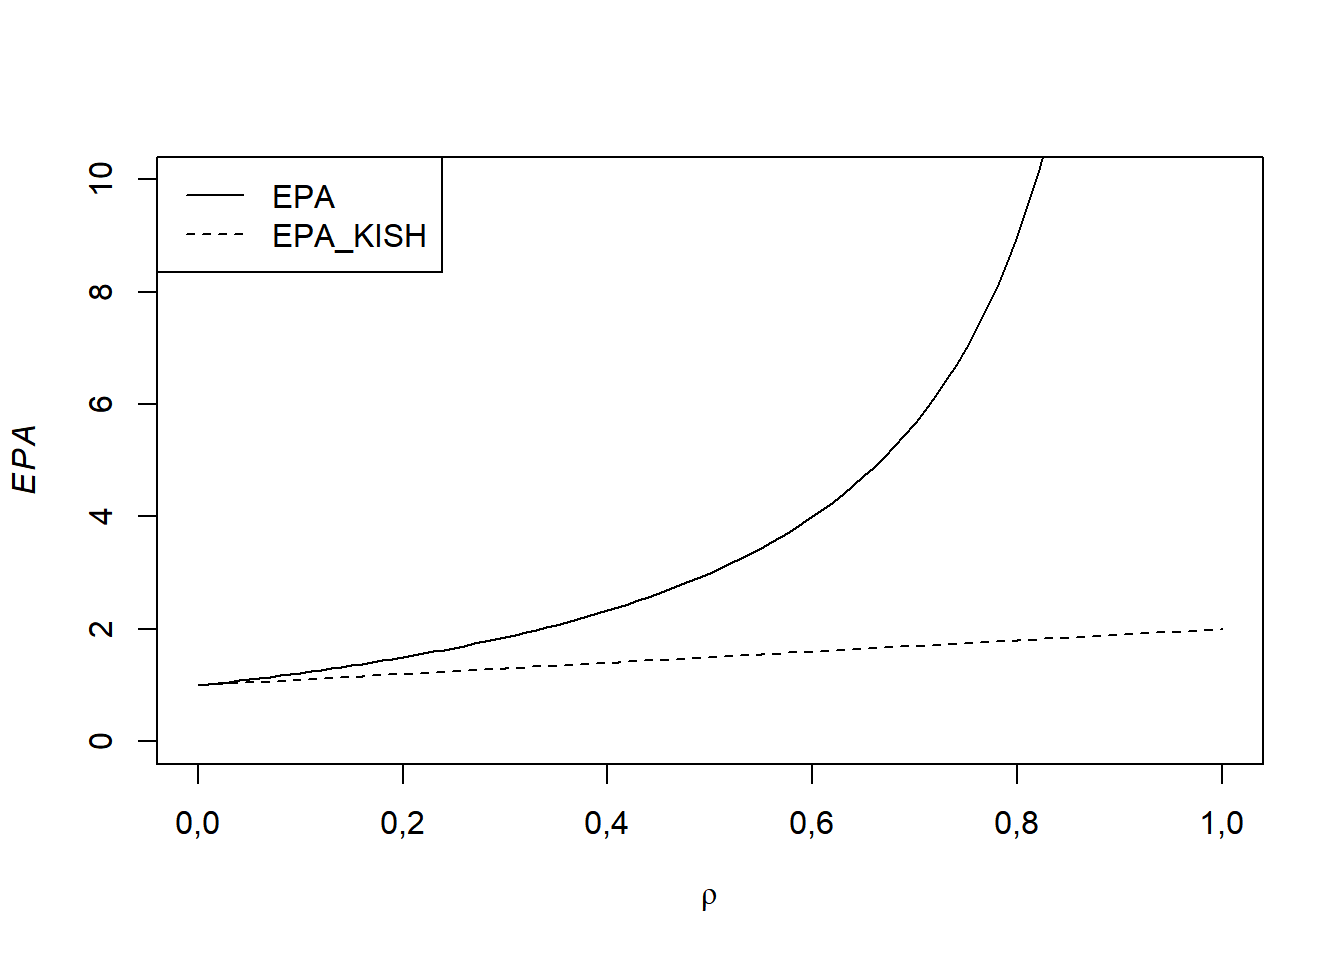
\includegraphics{04-Cap4_files/figure-latex/epacong-1.pdf}
\caption{\label{fig:epacong}Valores de EPA e EPA de Kish para conglomeração}
\end{figure}

Este exemplo ilustra bem dois aspectos distintos do uso de medidas como
o efeito de plano amostral. O primeiro é que as duas medidas são
distintas,
\texttt{embora\ os\ respectivos\ estimadores\ baseados\ numa\ particular\ amostra\ coincidam}.
No caso particular deste exemplo, o
\(\mathbf{EPA}_{Kish}\left( \hat{\theta}\right)\) cresce pouco com o
valor do coeficiente de correlação intraclasse \(\rho\), o que implica
que um plano amostral conglomerado como o adotado (seleção ao acaso de
um par da população) seria menos eficiente que um plano amostral
aleatório simples (seleção de duas unidades ao acaso da população), mas
a perda de eficiência seria modesta. Já se o interesse é medir, a
posteriori, o efeito da má especificação do plano amostral no estimador
de variância, o impacto, medido pelo
\(\mathbf{EPA}\left( \hat{\theta},v_{0}\right)\), seria muito maior.

Vale ainda notar que o \(\mathbf{EPA}\left( \hat{\theta},v_{0}\right)\)
mede o impacto da má especificação do plano amostral ou do modelo para a
estrutura populacional. Neste exemplo, ignorar a estrutura da população
(o fato de que as observações são pareadas) poderia provocar
subestimação da variância do estimador de média, que seria tanto maior
quanto maior fosse o coeficiente de correlação intraclasse \(\rho\).
Efeitos como esse são comuns também devido ao planejamento amostral,
mesmo em populações onde a conglomeração é imposta artificialmente pelo
amostrista.

\section{Intervalos de Confiança e Testes de Hipóteses}\label{icth}

A partir da estimativa pontual \(\hat{\theta}\) de um parâmetro
\(\theta\) (da população finita ou do modelo de superpopulação) é
possível construir um intervalo de confiança de nível de confiança
aproximado \(\left( 1-\alpha \right)\) a partir da distribuição
assintótica de \[
t_{0}=\frac{\hat{\theta}-\theta }{v_{0}^{1/2}} 
\] que, sob a hipótese de que as observações são IID, frequentemente é
\(N\left( 0;1\right)\).

Neste caso, um intervalo de confiança de nível de confiança aproximado
\(\left( 1-\alpha \right)\) é dado por
\(\left[ \hat{\theta}-z_{\alpha /2}v_{0}^{1/2},\hat{\theta}+z_{\alpha /2}v_{0}^{1/2}\right]\),
onde \(z_{\alpha }\) é definido por
\(\int_{z_{\alpha }}^{+\infty }\varphi\left( t\right) dt=\alpha\) , onde
\(\varphi\) é a função de densidade da distribuição normal padrão.

Vamos analisar o efeito de um plano amostral complexo sobre o intervalo
de confiança. No caso de um plano amostral complexo, a distribuição que
é aproximadamente normal é a de \[
\frac{\hat{\theta}-\theta }{\left[ \widehat{V}_{VERD}\left( \hat{\theta}\right) \right] ^{1/2}}. 
\]

Por outro lado, para obter a variância da distribuição assintótica de
\(t_{0}\) note que \[
\frac{\hat{\theta}-\theta }{v_{0}^{1/2}}=\frac{\hat{\theta}-\theta }{\left[ 
\widehat{V}_{VERD}\left( \hat{\theta}\right) \right] ^{1/2}}\times \frac{
\left[ \widehat{V}_{VERD}\left( \hat{\theta}\right) \right] ^{1/2}}{
v_{0}^{1/2}}\;. 
\]

Como o primeiro fator tende para uma \(N\left( 0;1\right)\), a variância
assintótica de \(t_{0}\) é aproximadamente igual ao quadrado do segundo
fator, isto é, a
\(\frac{\widehat{V}_{VERD}\left( \hat{\theta}\right) }{v_{0}}\) que é um
estimador para \(\mathbf{EPA}\left( \hat{\theta},v_{0}\right)\). Porém
quando a amostra é grande esse valor aproxima o
\(\mathbf{EPA}\left( \hat{\theta},v_{0}\right) =\frac{V_{VERD}\left( \hat{\theta}\right) }{E_{VERD}\left( v_{0}\right) }\),
pois \(v_{0}\) é aproximadamente igual a \(E_{VERD}\left( v_{0}\right)\)
e \(\widehat{V}_{VERD}\left( \hat{\theta}\right)\) é aproximadamente
igual a \(V_{VERD}\left( \hat{\theta}\right)\). Logo temos que a
distribuição assintótica verdadeira de \(t_{0}\) é dada por \[
t_{0}\sim N\left[ 0;\mathbf{EPA}\left( \hat{\theta},v_{0}\right)
\right] \;. 
\]

Dependendo do valor de \(\mathbf{EPA}\left( \hat{\theta},v_{0}\right)\),
o intervalo de confiança baseado na distribuição assintótica verdadeira
de \(t_{0}\) pode ser bem distinto daquele baseado na distribuição
assintótica obtida sob a hipótese de observações IID. Em geral, a
probabilidade de cobertura assintótica do intervalo
\(\left[\hat{\theta}-z_{\alpha /2}v_{0}^{1/2}, \hat{\theta}+z_{\alpha/2}v_{0}^{1/2}\right]\)
será aproximadamente igual a

\[
2\Phi \left( z_{\alpha /2}/\left[ \mathbf{EPA}\left( \hat{\theta}
,v_{0}\right) \right] ^{1/2}\right) -1\;\;, 
\] onde \(\Phi\) é a função de distribuição acumulada de uma
\(N\left( 0;1\right)\). Calculamos esta probabilidade para alguns
valores do \(\mathbf{EPA}\), que apresentamos na Tabela
\ref{tab:procob}.

\begin{longtable}[]{@{}lll@{}}
\caption{\label{tab:procob} Probabilidades de cobertura para níveis nominais
de 95\% e 99\%}\tabularnewline
\toprule
\(\mathbf{EPA}\left( \hat{\theta},v_{0}\right)\) & \(1-\alpha=0.95\) &
\(1-\alpha=0.99\)\tabularnewline
\midrule
\endfirsthead
\toprule
\(\mathbf{EPA}\left( \hat{\theta},v_{0}\right)\) & \(1-\alpha=0.95\) &
\(1-\alpha=0.99\)\tabularnewline
\midrule
\endhead
0,90 & 0,96 & 0,99\tabularnewline
0,95 & 0,96 & 0,99\tabularnewline
1,0 & 0,95 & 0,99\tabularnewline
1,5 & 0,89 & 0,96\tabularnewline
2,0 & 0,83 & 0,93\tabularnewline
2,5 & 0,78 & 0,90\tabularnewline
3,0 & 0,74 & 0,86\tabularnewline
3,5 & 0,71 & 0,83\tabularnewline
4,0 & 0,67 & 0,80\tabularnewline
\bottomrule
\end{longtable}

À medida que o valor do \(\mathbf{EPA}\left( \hat{\theta},v_{0}\right)\)
aumenta, a probabilidade real de cobertura diminui, sendo menor que o
valor nominal para valores de
\(\mathbf{EPA}\left( \hat{\theta},v_{0}\right)\) maiores que 1.

Utilizando a correspondência existente entre intervalos de confiança e
testes de hipóteses, podemos derivar os níveis de significância nominais
e reais subtraindo de \(1\) os valores da Tabela \ref{tab:procob}. Por
exemplo, para \(\alpha =0,05\) e
\(\mathbf{EPA}\left( \hat{\theta},v_{0}\right) =2\), o nível de
significância real seria aproximadamente \(1-0,83=0,17\).

\BeginKnitrBlock{example}
\protect\hypertarget{exm:exebin}{}{\label{exm:exebin} }Teste de hipótese
sobre proporção
\EndKnitrBlock{example} Vamos considerar um exemplo hipotético de teste
de hipótese sobre uma proporção, semelhante ao de \citep{Sud76},
apresentado em p.~196, \citep{lethonen}. Uma amostra de \(m=50\)
conglomerados é extraída de uma grande população de empresas industriais
(conglomerados). Suponhamos que cada empresa \(i=1,\ldots ,50\) da
amostra tenha \(n_{i}=20\) empregados. O tamanho total da amostra de
empregados (unidades elementares) é \(n=\sum_{i}n_{i}=1.000\). Queremos
estudar o acesso dos trabalhadores das empresas a planos de saúde.

Usando-se conhecimento do ano anterior, foi estabelecida a hipótese de
que a proporção de trabalhadores cobertos por planos de saúde é
\(80\%\), ou seja \(H_{0}:p=p_{0}=0,8\). Vamos adotar o nível de
significância \(\alpha =5\%\).

A estimativa obtida na pesquisa foi \(\widehat{p}=n_{A}/n=0,84\), onde
\(n_{A}=840\) é o número de trabalhadores na amostra com acesso a planos
de saúde. Ignorando o plano amostral e a conglomeração das unidades
elementares na população, podemos considerar um teste binomial e usar a
aproximação normal \(N(0;1)\) para a estatística de teste

\begin{equation}
Z=|\widehat{p}-p_{0}|/\sqrt{p_{0}\left( 1-p_{0}\right) /n},  \label{eq:epa4}
\end{equation}

onde o denominador é o desvio padrão da estimativa \(\widehat{p}\) sob a
hipótese nula.

Vamos calcular o valor da estatística \(Z\), supondo que tenha sido
usada amostragem aleatória simples com reposição (AASC) de empregados.
Vamos também considerar uma abordagem baseada no plano amostral de
conglomerados. O desvio padrão de \(\widehat{p}\), no denominador de
\(Z\), será baseado na hipótese de distribuição binomial, com tamanhos
amostrais diferentes para as duas abordagens.

Para o teste baseado na amostragem aleatória simples, ignoramos a
conglomeração e usamos na fórmula do desvio padrão o tamanho total da
amostra de unidades elementares (empregados), isto é, \(n=1.000\). O
valor da estatística de teste \(Z\) definida em \eqref{eq:epa4} é,
portanto,

\begin{equation}
Z_{bin}=|0,84-0,8|/\sqrt{0,8\left( 1-0,8\right) /1.000}=3,162>Z_{0,025}=1,96
\label{eq:epa5}
\end{equation}

onde \(\sqrt{0,8\left( 1-0,8\right) /1.000}=0,0126\) é o desvio padrão
de \(\widehat{p}\) sob a hipótese nula. Este~resultado sugere a rejeição
da hipótese \(H_{0}\).

Por outro lado, é razoável admitir que se uma empresa for coberta por
plano de saúde, cada empregado dessa empresa terá acesso ao plano. Essa
é uma informação importante que foi ignorada no teste anterior. De fato,
selecionar mais de uma pessoa numa empresa não aumenta nosso
conhecimento sobre a cobertura por plano de saúde no local. Portanto, o
\texttt{tamanho\ efetivo} da amostra é \(\overline{n}=50\) , em
contraste com o valor \(1.000\) usado no teste anterior. O termo
\texttt{tamanho\ efetivo} foi introduzido em \citep{Kish65} para
designar o tamanho de uma amostra aleatória simples necessário para
estimar \(p\) com a mesma precisão obtida por uma amostra conglomerada
de tamanho \(n\) (neste caso, igual a \(1.000\)) unidades elementares.

Usando o tamanho efetivo de amostra, temos a estatística de teste
baseada no plano amostral verdadeiro \[
Z_{p}=|\widehat{p}-p_{0}|/\sqrt{p_{0}\left( 1-p_{0}\right) /50}=0,707 ,
\] onde o valor \(\sqrt{0,8\left( 1-0,8\right) /50}=0,0566\) é muito
maior que o valor do desvio padrão obtido no teste anterior. Portanto, o
valor observado de \(Z_{p}\) é menor que o de \(Z_{bin}\), e o novo
teste sugere a não rejeição da mesma hipótese nula.

Neste exemplo, portanto, se verifica que ignorar a conglomeração pode
induzir a uma decisão incorreta de rejeitar a hipótese nula, quando a
mesma não seria rejeitada se o plano amostral fosse corretamente
incorporado na análise. Efeitos desse tipo são mais difíceis de
antecipar para inferência analítica, particularmente quando os planos
amostrais empregados envolvem combinação de estratificação,
conglomeração e probabilidades desiguais de seleção. Por essa razão, a
recomendação é procurar sempre considerar o plano amostral na análise,
ao menos como forma de verificar se as conclusões obtidas por formas
ingênuas de análise ignorando os pesos e plano amostral são as mesmas.

\section{Efeitos Multivariados de Plano
Amostral}\label{efeitos-multivariados-de-plano-amostral}

O conceito de efeito de plano amostral introduzido em \eqref{eq:epa2} é
relativo a inferências sobre um parâmetro univariado \(\theta\).
Consideremos agora o problema de estimação de um vetor
\(\mathbf{\theta}\) de \(K\) parâmetros. Seja \(\mathbf{\hat{\theta}}\)
um estimador de \(\mathbf{\theta}\) e seja \(\mathbf{V}_{0}\) um
estimador da matriz \(K\times K\) de covariância de
\(\mathbf{\hat{\theta}}\), baseado nas hipóteses de independência e
igualdade de distribuição das observações (IID), ou equivalentemente, de
amostragem aleatória simples com reposição (AASC). é possível
generalizar a equação \eqref{eq:epa2}, definindo o
\texttt{efeito\ multivariado\ do\ plano\ amostral\ de}
\(\mathbf{\hat{\theta}}\) \textbf{e} \(\mathbf{V}_{0}\) como

\begin{equation}
\mathbf{EMPA}(\mathbf{\hat{\theta},V}_{0})=\mathbf{\Delta =E}_{VERD}\left( 
\mathbf{V}_{0}\right) ^{-1}\mathbf{V}_{VERD}(\mathbf{\hat{\theta}),}
\label{eq:epa6}
\end{equation}

onde \(\mathbf{E}_{VERD}\left( \mathbf{V}_{0}\right)\) é o valor
esperado de \(\mathbf{V}_{0}\) e,
\(\mathbf{V}_{VERD}(\mathbf{\hat{\theta})}\) é a matriz de covariância
de \(\mathbf{\hat{\theta}}\), ambas calculadas com respeito `\{a\}
distribuição de aleatorização induzida pelo plano amostral efetivamente
utilizado, ou alternativamente sob o \texttt{modelo\ correto}.

Os autovalores \(\delta _{1}\geq \ldots \geq \delta _{K}\) da matriz
\(\mathbf{\Delta }\) são denominados
\texttt{efeitos\ generalizados\ do\ plano\ amostral}. A partir deles, e
utilizando resultados padrões de teoria das matrizes (p.64,
\citep{Johnson}) é possível definir limitantes para os efeitos
(univariados) do plano amostral para combinações lineares
\(\mathbf{c}^{^{\prime }}\widehat{\mathbf{\theta }}\) das componentes de
\(\widehat{\mathbf{\theta }}\). Temos os seguintes resultados:

\begin{eqnarray*}
\delta _{1} &=&\max \mathbf{EPA}(\mathbf{c}^{^{\prime }}\widehat{\mathbf{
\theta }}\mathbf{,c}^{^{\prime }}\mathbf{V}_{0}\mathbf{c)}, \\
\delta _{K} &=&\min \mathbf{EPA}(\mathbf{c}^{^{\prime }}\widehat{\mathbf{\theta }}\mathbf{,c}^{^{\prime }}\mathbf{V}_{0}\mathbf{c)}.
\end{eqnarray*}

No caso particular onde \(\mathbf{\Delta =I}_{K\times K}\) , temos
\(\delta_{1}=\ldots =\delta _{K}=1\) e os efeitos (univariados) do plano
amostral das combinações lineares para componentes de
\(\mathbf{\hat{\theta}}\) são todos iguais a \(1\). Para ilustrar esse
conceito, vamos reconsiderar o Exemplo \ref{exm:deffuni} de estimação de
médias com amostragem estratificada desproporcional anteriormente
apresentado, mas agora considerando a natureza multivariada do problema
(há duas variáveis de pesquisa).

\BeginKnitrBlock{example}
\protect\hypertarget{exm:deffmult}{}{\label{exm:deffmult} }Efeitos
Multivariados do Plano Amostral para as médias de Salários e de Receitas
\EndKnitrBlock{example}

Vamos considerar as variáveis Salário (em R\$ \(1.000\)) e Receita (em
R\$ \(1.000.000\)) definidas na população de empresas do Exemplo
\ref{exm:deffuni} e calcular a matriz
\(\mathbf{EMPA}\left( \mathbf{\hat{\theta},V}_{0}\right)\), onde
\(\mathbf{\hat{\theta}=}\left( \overline{SAL}_{w},\overline{REC}_{w}\right) ^{\prime }\).
Neste exemplo, os dados populacionais são conhecidos, e portanto podemos
calcular a covariância dos estimadores
\(\left( \overline{SAL}_{w},\overline{REC}_{w}\right)\). Usando a mesma
notação do Exemplo \ref{exm:deffuni}, temos que \[
COV_{AES}(\overline{SAL}_{w},\overline{REC}_{w}\mathbf{)=}\sum\limits_{h=1}^{2}W_{h}^{2}\frac{\left( 1-f_{h}\right) }{n_{h}}S_{SAL,REC}^{\left( h\right) } 
\] onde \[
S_{SAL,REC}^{\left( h\right) }=\frac{1}{N_{h}-1}\sum\limits_{i\in
U_{h}}\left( SAL_{hi}-\overline{SAL}_{h}\right) \left( REC_{hi}-\overline{REC
}_{h}\right) \;. 
\]

Substituindo os valores conhecidos na população das variáveis
\(SAL_{hi}\) e \(REC_{hi}\), obtemos para esta covariância o valor \[
COV_{AES}(\overline{SAL}_{w},\overline{REC}_{w}\mathbf{)=\;}3.2358
\] e portanto a matriz de variância
\(\mathbf{V}_{AES}(\overline{SAL}_{w},\overline{REC}_{w})\) dos
estimadores ponderados da média fica igual a

\begin{verbatim}
       SAL   REC
SAL 244,18 3,236
REC   3,24 0,435
\end{verbatim}

onde os valores das variâncias em \eqref{eq:epa7} foram os calculados no
Exemplo \ref{exm:deffuni} e coincidem, respectivamente, com os valores
usados nos numeradores de
\(\mathbf{EPA}\left( \overline{SAL}_{w}\right)\) e de
\(\mathbf{EPA}\left( \overline{REC}_{w}\right)\) lá apresentados. Para
calcular o \(\mathbf{EMPA}(\mathbf{\hat{\theta},V}_{0})\) é preciso
agora obter \(\mathbf{E}_{VERD}\left(\mathbf{V}_{0}\right)\).

Neste exemplo, a matriz de efeito do plano amostral
\(\mathbf{EMPA}(\mathbf{\hat{\theta},V}_{0})=\mathbf{\Delta }\) pode
também ser calculada através de simulação, de modo análogo ao que foi
feito no Exemplo \ref{exm:deffuni}. Para isto, foram utilizadas outras
\(500\) amostras de tamanho \(60\) segundo o plano amostral descrito no
Exemplo \ref{exm:deffuni}. Para cada uma das \(500\) amostras foram
calculadas estimativas:

\begin{enumerate}
\def\labelenumi{\arabic{enumi}.}
\item
  da variância da média amostral ponderada do salário e da receita
  assumindo observações IID;
\item
  da covariância entre médias ponderadas do salário e da receita
  assumindo observações IID;
\item
  da variância da média amostral ponderada do salário e da receita
  considerando o plano amostral verdadeiro;
\item
  da covariância entre médias ponderadas do salário e da receita
  considerando o plano amostral verdadeiro.
\end{enumerate}

A partir da simulação foram obtidos os seguintes resultados:

\begin{itemize}
\tightlist
\item
  A matriz de covariância das médias amostrais ponderadas de salário e
  da receita, assumindo observações IID \(E_{AES}\left(V_{0}\right)\):
\end{itemize}

\begin{verbatim}
       SAL   REC
SAL 1720,0 26,78
REC   26,8  1,21
\end{verbatim}

\begin{itemize}
\tightlist
\item
  A matriz de covariância das médias ponderadas de salário e da receita
  considerando o plano amostral verdadeiro
  \(V_{AES}\left(\hat{\theta}\right)\):
\end{itemize}

\begin{verbatim}
       SAL   REC
SAL 245,19 3,172
REC   3,17 0,401
\end{verbatim}

\begin{itemize}
\tightlist
\item
  A matriz \(\Delta\) definida em \eqref{eq:epa6}
\end{itemize}

\(\Delta = \left[ E_{AES}\left( V_{0}\right)\right]^{-1}V_{AES}(\hat{\theta})\)

\begin{verbatim}
        sal      rec
[1,]  0,155 -0,00509
[2,] -0,817  0,44506
\end{verbatim}

Os autovalores 1 e 1,02 de \(\mathbf{\Delta}\) fornecem os efeitos
generalizados do plano amostral.

Da mesma forma que o \(\mathbf{EPA}\left( \hat{\theta},v_{0}\right)\)
definido em \eqref{eq:epa2} para o caso uniparamétrico foi utilizado para
corrigir níveis de confiança de intervalos e níveis de significância de
testes, o \(\mathbf{EMPA}(\mathbf{\hat{\theta},V}_{0})\) definido em
\eqref{eq:epa6} pode ser utilizado para corrigir níveis de confiança de
regiões de confiança e níveis de significância de testes de hipóteses no
caso multiparamétrico. Para ilustrar, vamos considerar o problema de
testar a hipótese \(H_{0}:\mathbf{\mu }=\mathbf{\mu }_{0}\), onde
\(\mathbf{\mu }\) é o vetor de médias de um vetor de variáveis de
pesquisa \(\mathbf{y}\). A estatística de teste usualmente adotada para
este caso é a \(T^{2}\) de Hottelling dada por

\begin{equation}
T^{2}=n\left( \mathbf{\bar{y}-\mu }_{0}\right) ^{^{\prime }}\mathbf{S}
_{y}^{-1}\left( \mathbf{\bar{y}-\mu }_{0}\right) , \label{eq:epa11} 
\end{equation}

onde

\begin{eqnarray*}
\mathbf{\bar{y}} &=&\frac{1}{n}\sum\limits_{i\in s}\mathbf{y}_{i},\quad 
\mathbf{S}_{y}=\frac{1}{n-1}\sum\limits_{i\in s}\left( \mathbf{y}_{i}-
\mathbf{\bar{y}}\right) \left( \mathbf{y}_{i}-\mathbf{\bar{y}}\right)
^{^{\prime }},\mbox{ e } \\
\mathbf{\mu }_{0} &=&\left( \mu _{10},\mu _{20},\ldots ,\mu _{K0}\right)
^{^{\prime }}\;\;.
\end{eqnarray*}

Se as observações \(\mathbf{y}_{i}\) são IID normais, a estatística
\(T^{2}\) tem a distribuição
\(\frac{\left( n-1\right) }{\left( n-K\right)}\mathbf{F}\left( K;n-K\right)\)
sob \(H_{0}\), onde \(\mathbf{F}\left( K;n-K\right)\) denota uma
variável aleatória com distribuição \(\mathbf{F}\) com \(K\) e
\(\left( n-K\right)\) graus de liberdade. Mesmo se as observações
\(\mathbf{y}_{i}\) não forem normais, \(T^{2}\) tem distribuição
assintótica \(\chi ^{2}\left(K\right)\) quando \(n\rightarrow \infty\),
\citep{Johnson}, p.191.

Contudo, se for utilizado um plano amostral complexo, \(T^{2}\) tem
aproximadamente a distribuição da variável \(\sum\limits_{i=1}^{K}\)
\(\delta _{i}Z_{i}^{2}\), onde \(Z_{1},\ldots ,Z_{K}\) são variáveis
aleatórias independentes com distribuição normal padrão e os
\(\delta _{i}\) são os autovalores da matriz
\(\mathbf{\Delta }=\Sigma _{AAS}^{-1}\Sigma\), onde
\(\Sigma _{AAS}=E_{p}(\mathbf{S}_{y}/n)\) e
\(\Sigma =V_{p}(\mathbf{\bar{y})}\).

Vamos analisar o efeito do plano amostral sobre o nível de significância
deste teste. Para simplificar, consideremos o caso em que
\(\delta _{1}=\ldots =\delta _{K}=\delta\). Neste caso, o nível de
significância real é dado aproximadamente por

\begin{equation}
P\left(\chi ^{2}\left( K\right) >\chi _{\alpha }^{2}\left( K\right) /\delta\right)  \label{eq:epa12}
\end{equation}

onde \(\chi _{\alpha }^{2}\left( K\right)\) é o quantil superior
\(\alpha\) de uma distribuição \(\chi ^{2}\) com \(K\) graus de
liberdade, isto é, o valor tal que
\(P\left[ \chi ^{2}\left( K\right) >\chi _{\alpha}^{2}\left( K\right) \right] =\alpha\)
.

A Tabela \ref{tab:nivsig} apresenta os níveis de significância reais
para \(\alpha =5\%\) para vários valores de \(K\) e \(\delta\). Mesmo
quando os valores dos \(\delta _{i}\) são distintos, os valores da
Tabela \ref{tab:nivsig} podem ser devidamente interpretados. Para isso,
consideremos o \(p\)valor do teste da hipótese
\(H_{0}:\mathbf{\mu }=\mathbf{\mu }_{0}\), sob a hipótese de amostragem
aleatória simples com reposição e sob o plano amostral efetivamente
utilizado. Por definição este valor é dado por \[
p\mbox{valor}_{AAS}\left( \mathbf{\bar{y}}\right) =P\left[ \chi ^{2}\left(
K\right) >\left( \mathbf{\bar{y}-\mu }_{0}\right) ^{^{\prime }}\mathbf{
\Sigma }_{AAS}^{-1}\left( \mathbf{\bar{y}-\mu }_{0}\right) \right] 
\] e \(H_{0}\) é rejeitada com nível de significância \(\alpha\) se
valor-\(p\) \(_{AAS}<\alpha\).

O verdadeiro valor-\(p\) pode ser definido analogamente como

\begin{equation}
p\mbox{valor}_{VERD}\left( \mathbf{\bar{y}}\right) =P\left[ \chi ^{2}\left(K\right) >\left( \mathbf{\bar{y}-\mu }_{0}\right) ^{^{\prime }}\mathbf{\Sigma }_{VERD}^{-1}\left( \mathbf{\bar{y}-\mu }_{0}\right) \right] \;.
\label{eq:epa13}
\end{equation}

Os valores na Tabela \ref{tab:nivsig} podem ser usados para quantificar
a diferença entre estes valores-\(p\). Consideremos a região crítica do
teste de nível \(\alpha\) baseado na hipótese de AAS:

\begin{eqnarray}
RC_{AAS}\left( \mathbf{\bar{y}}\right) &=&\left\{ \mathbf{\bar{y}:}\left( 
\mathbf{\bar{y}-\mu }_{0}\right) ^{^{\prime }}\mathbf{\Sigma }
_{AAS}^{-1}\left( \mathbf{\bar{y}-\mu }_{0}\right) >\chi _{\alpha
}^{2}\left( K\right) \right\} \label{eq:epa14}  \\
&=&\left\{ \mathbf{\bar{y}:}p\mbox{valor}_{AAS}\left( \mathbf{\bar{y}}
\right) <\alpha \right\}.  \nonumber
\end{eqnarray}

Pode-se mostrar que o máximo de
\(p\)valor\(_{VERD}\left( \mathbf{\bar{y}}\right)\) quando
\(\mathbf{\bar{y}}\) pertence à
\(RC_{AAS}\left( \mathbf{\bar{y}}\right)\) é dado por:

\begin{equation}
\max_{\mathbf{\bar{y}\in }RC_{AAS}\left( \mathbf{\bar{y}}\right) }p
\mbox{valor}_{VERD}\left( \mathbf{\bar{y}}\right) =P\left( \chi ^{2}\left(K\right) >\chi _{\alpha }^{2}\left( K\right) /\delta _{1}\right).
\label{eq:epa15}
\end{equation}

Observe que o segundo membro de \eqref{eq:epa15} é da mesma forma que o
segundo membro de \eqref{eq:epa12}. Logo, os valores da Tabela
\ref{tab:nivsig} podem ser interpretados como valores máximos de
\(p\)valor\(_{VERD}\left( \mathbf{\bar{y}}\right)\) para
\(\mathbf{\bar{y}}\) na região
\(RC_{AAS}\left(\mathbf{\bar{y}}\right)\), considerando-se
\(\delta_{1}\) no lugar de \(\delta\).

\begin{longtable}[]{@{}cllrr@{}}
\caption{\label{tab:nivsig} Níveis de significância (\%) verdadeiros do
teste T2 para o nível nominal de 5\% assumindo autovalores iguais a
\(\delta\).}\tabularnewline
\toprule
& & K & &\tabularnewline
\midrule
\endfirsthead
\toprule
& & K & &\tabularnewline
\midrule
\endhead
\(\delta\) & 1 & 2 & 3 & 4\tabularnewline
0,9 & 4 & 4 & 3 & 3\tabularnewline
1,0 & 5 & 5 & 5 & 5\tabularnewline
1,5 & 11 & 14 & 16 & 19\tabularnewline
2,0 & 17 & 22 & 27 & 32\tabularnewline
2,5 & 22 & 30 & 37 & 44\tabularnewline
3,0 & 26 & 37 & 46 & 53\tabularnewline
\bottomrule
\end{longtable}

\section{Laboratório de R}\label{laboratorio-de-r-1}

Utilizando o R, obtemos a seguir alguns resultados descritos nos
Exemplos \ref{exm:deffuni} e \ref{exm:deffmult}. Na simulação, usamos a
library \texttt{sampling} \citep{R-sampling} para gerar amostras
estratificadas de tamanho 30, com estratos definidos na Tabela
\ref{tab:estempr}, para obter os valores nas Tabelas \ref{tab:proestmed}
e \ref{tab:varest}.

\begin{Shaded}
\begin{Highlighting}[]
\CommentTok{# carrega library}
\KeywordTok{library}\NormalTok{(survey)}
\CommentTok{# carrega dados}
\KeywordTok{library}\NormalTok{(anamco)}
\NormalTok{popul_dat <-}\StringTok{ }\NormalTok{popul}
\NormalTok{N <-}\StringTok{ }\KeywordTok{nrow}\NormalTok{(popul_dat)}
\NormalTok{n1 <-}\StringTok{ }\DecValTok{30}
\NormalTok{n2 <-}\StringTok{ }\DecValTok{30}
\NormalTok{nh =}\StringTok{ }\KeywordTok{c}\NormalTok{(n1, n2)}
\NormalTok{n <-}\StringTok{ }\KeywordTok{sum}\NormalTok{(nh)}
\NormalTok{Nh <-}\StringTok{ }\KeywordTok{table}\NormalTok{(popul_dat}\OperatorTok{$}\NormalTok{estrat)}
\NormalTok{fh <-}\StringTok{ }\NormalTok{nh}\OperatorTok{/}\NormalTok{Nh}
\NormalTok{Wh <-}\StringTok{ }\NormalTok{Nh}\OperatorTok{/}\NormalTok{N}
\NormalTok{f <-}\StringTok{ }\NormalTok{n}\OperatorTok{/}\NormalTok{N}
\NormalTok{popul_dat}\OperatorTok{$}\NormalTok{sal <-}\StringTok{ }\NormalTok{popul_dat}\OperatorTok{$}\NormalTok{sal}\OperatorTok{/}\DecValTok{1000}
\NormalTok{popul_dat}\OperatorTok{$}\NormalTok{rec <-}\StringTok{ }\NormalTok{popul_dat}\OperatorTok{$}\NormalTok{rec}\OperatorTok{/}\FloatTok{1e+06}
\KeywordTok{library}\NormalTok{(sampling)}
\CommentTok{# define espaços para salvar resultados}
\NormalTok{est_aas <-}\StringTok{ }\KeywordTok{c}\NormalTok{(}\DecValTok{0}\NormalTok{, }\DecValTok{0}\NormalTok{)}
\NormalTok{est_aes <-}\StringTok{ }\KeywordTok{c}\NormalTok{(}\DecValTok{0}\NormalTok{, }\DecValTok{0}\NormalTok{)}
\NormalTok{cov_mat_aas_est <-}\StringTok{ }\KeywordTok{matrix}\NormalTok{(}\DecValTok{0}\NormalTok{, }\DecValTok{2}\NormalTok{, }\DecValTok{2}\NormalTok{)}
\NormalTok{cov_mat_aes_est <-}\StringTok{ }\KeywordTok{matrix}\NormalTok{(}\DecValTok{0}\NormalTok{, }\DecValTok{2}\NormalTok{, }\DecValTok{2}\NormalTok{)}
\KeywordTok{set.seed}\NormalTok{(}\DecValTok{123}\NormalTok{)}
\CommentTok{# gera amostras com dois estratos de tamanho 30}
\ControlFlowTok{for}\NormalTok{ (i }\ControlFlowTok{in} \DecValTok{1}\OperatorTok{:}\DecValTok{500}\NormalTok{) \{}
\NormalTok{  s <-}\StringTok{ }\KeywordTok{strata}\NormalTok{(popul_dat, }\StringTok{"estrat"}\NormalTok{, }\KeywordTok{c}\NormalTok{(}\DecValTok{30}\NormalTok{, }\DecValTok{30}\NormalTok{), }\DataTypeTok{method =} \StringTok{"srswor"}\NormalTok{)}
\NormalTok{  dados <-}\StringTok{ }\KeywordTok{getdata}\NormalTok{(popul_dat, s)}
  \CommentTok{# média amostral de salário e de receita}
\NormalTok{  est_aas <-}\StringTok{ }\NormalTok{est_aas }\OperatorTok{+}\StringTok{ }\KeywordTok{c}\NormalTok{(}\KeywordTok{mean}\NormalTok{(dados}\OperatorTok{$}\NormalTok{sal), }\KeywordTok{mean}\NormalTok{(dados}\OperatorTok{$}\NormalTok{rec))}
  \CommentTok{# estimador v0}
\NormalTok{  cov_mat_aas_est <-}\StringTok{ }\NormalTok{cov_mat_aas_est }\OperatorTok{+}\StringTok{ }\NormalTok{(}\DecValTok{1} \OperatorTok{-}\StringTok{ }\NormalTok{f) }\OperatorTok{*}\StringTok{ }\KeywordTok{cov}\NormalTok{(}\KeywordTok{cbind}\NormalTok{(dados}\OperatorTok{$}\NormalTok{sal, }
\NormalTok{    dados}\OperatorTok{$}\NormalTok{rec))}\OperatorTok{/}\NormalTok{n}
  
  \CommentTok{# vhat_aes estimador não-viciado}
\NormalTok{  popul_plan <-}\StringTok{ }\KeywordTok{svydesign}\NormalTok{(}\OperatorTok{~}\DecValTok{1}\NormalTok{, }\DataTypeTok{strata =} \OperatorTok{~}\NormalTok{estrat, }\DataTypeTok{data =}\NormalTok{ dados, }
    \DataTypeTok{fpc =} \OperatorTok{~}\NormalTok{Prob)}
  \CommentTok{# estimador não-viciado da média de salario e receita}
\NormalTok{  sal_rec_aes_est <-}\StringTok{ }\KeywordTok{svymean}\NormalTok{(}\OperatorTok{~}\NormalTok{sal }\OperatorTok{+}\StringTok{ }\NormalTok{rec, popul_plan)}
\NormalTok{  est_aes <-}\StringTok{ }\NormalTok{est_aes }\OperatorTok{+}\StringTok{ }\KeywordTok{coef}\NormalTok{(sal_rec_aes_est)}
\NormalTok{  cov_mat_aes_est <-}\StringTok{ }\NormalTok{cov_mat_aes_est }\OperatorTok{+}\StringTok{ }\KeywordTok{attr}\NormalTok{(sal_rec_aes_est, }
    \StringTok{"var"}\NormalTok{)}
\NormalTok{\}}

\CommentTok{# média populacional}

\NormalTok{med_pop <-}\StringTok{ }\KeywordTok{round}\NormalTok{(}\KeywordTok{c}\NormalTok{(}\KeywordTok{mean}\NormalTok{(popul_dat}\OperatorTok{$}\NormalTok{sal), }\KeywordTok{mean}\NormalTok{(popul_dat}\OperatorTok{$}\NormalTok{rec)),}\DecValTok{3}\NormalTok{)}


\CommentTok{# Calcula médias das estimativas na simulação}

\NormalTok{## Média das estimativas pontuais para as 500 amostras aas}
\NormalTok{mean_est_aas <-}\StringTok{ }\KeywordTok{round}\NormalTok{(est_aas}\OperatorTok{/}\DecValTok{500}\NormalTok{,}\DecValTok{3}\NormalTok{)}
\NormalTok{mean_est_aas}
\end{Highlighting}
\end{Shaded}

\begin{verbatim}
## [1] 163,50   4,17
\end{verbatim}

\begin{Shaded}
\begin{Highlighting}[]
\NormalTok{## Média das estimativas pontuais para as 500 amostras aes}
\NormalTok{mean_est_aes <-}\StringTok{ }\KeywordTok{round}\NormalTok{(est_aes}\OperatorTok{/}\DecValTok{500}\NormalTok{,}\DecValTok{3}\NormalTok{)}
\NormalTok{mean_est_aes}
\end{Highlighting}
\end{Shaded}

\begin{verbatim}
##   sal   rec 
## 78,07  2,06
\end{verbatim}

\begin{Shaded}
\begin{Highlighting}[]
\CommentTok{# Média das estimativas de matriz de covariância para as 500}
\CommentTok{# amostras aas}
\NormalTok{mean_cov_mat_aas_est <-}\StringTok{ }\KeywordTok{round}\NormalTok{(cov_mat_aas_est}\OperatorTok{/}\DecValTok{500}\NormalTok{, }\DecValTok{3}\NormalTok{)}
\NormalTok{mean_cov_mat_aas_est}
\end{Highlighting}
\end{Shaded}

\begin{verbatim}
##        [,1]  [,2]
## [1,] 1720,0 26,78
## [2,]   26,8  1,21
\end{verbatim}

\begin{Shaded}
\begin{Highlighting}[]
\CommentTok{# Média das estimativas de matriz de covariância para as 500}
\CommentTok{# amostras aes}
\NormalTok{mean_cov_mat_aes_est <-}\StringTok{ }\KeywordTok{round}\NormalTok{(cov_mat_aes_est}\OperatorTok{/}\DecValTok{500}\NormalTok{, }\DecValTok{3}\NormalTok{)}
\NormalTok{mean_cov_mat_aes_est}
\end{Highlighting}
\end{Shaded}

\begin{verbatim}
##        sal   rec
## sal 245,19 3,172
## rec   3,17 0,401
\end{verbatim}

\begin{Shaded}
\begin{Highlighting}[]
\NormalTok{## Matriz de covariância populacional}
\NormalTok{mat_cov_pop <-}\StringTok{ }\KeywordTok{by}\NormalTok{(popul_dat, popul_dat}\OperatorTok{$}\NormalTok{estrat, }\ControlFlowTok{function}\NormalTok{(t) }\KeywordTok{var}\NormalTok{(}\KeywordTok{cbind}\NormalTok{(t}\OperatorTok{$}\NormalTok{sal, }
\NormalTok{  t}\OperatorTok{$}\NormalTok{rec)))}
 


\NormalTok{## Matriz de covariância considerando o plano amostral}
\NormalTok{## verdadeiro}
\NormalTok{mat_cov_aleat_verd <-}\StringTok{ }\NormalTok{(Wh[}\DecValTok{1}\NormalTok{]}\OperatorTok{^}\DecValTok{2} \OperatorTok{*}\StringTok{ }\NormalTok{(}\DecValTok{1} \OperatorTok{-}\StringTok{ }\NormalTok{fh[}\DecValTok{1}\NormalTok{])}\OperatorTok{/}\NormalTok{nh[}\DecValTok{1}\NormalTok{]) }\OperatorTok{*}\StringTok{ }\NormalTok{mat_cov_pop[[}\DecValTok{1}\NormalTok{]] }\OperatorTok{+}\StringTok{ }
\StringTok{  }\NormalTok{(Wh[}\DecValTok{2}\NormalTok{]}\OperatorTok{^}\DecValTok{2} \OperatorTok{*}\StringTok{ }\NormalTok{(}\DecValTok{1} \OperatorTok{-}\StringTok{ }\NormalTok{fh[}\DecValTok{2}\NormalTok{])}\OperatorTok{/}\NormalTok{nh[}\DecValTok{2}\NormalTok{]) }\OperatorTok{*}\StringTok{ }\NormalTok{mat_cov_pop[[}\DecValTok{2}\NormalTok{]]}
\NormalTok{mat_cov_aleat_verd <-}\StringTok{ }\KeywordTok{round}\NormalTok{(mat_cov_aleat_verd,}\DecValTok{3}\NormalTok{)}


\NormalTok{## estimativa de efeitos generalizados do plano amostral}
\NormalTok{DELTA =}\StringTok{ }\KeywordTok{solve}\NormalTok{(mean_cov_mat_aas_est) }\OperatorTok\StringTok{ }\NormalTok{mean_cov_mat_aes_est}
\NormalTok{epa <-}\KeywordTok{round}\NormalTok{(}\KeywordTok{eigen}\NormalTok{(DELTA)}\OperatorTok{$}\NormalTok{values,}\DecValTok{3}\NormalTok{)}
\end{Highlighting}
\end{Shaded}

\BeginKnitrBlock{example}
\protect\hypertarget{exm:eqmean}{}{\label{exm:eqmean} }Teste da igualdade de
médias para duas populações
\EndKnitrBlock{example}

Para exemplificar o material descrito na Seção \ref{icth}, vamos
utilizar o data frame \texttt{amolim}, contendo dados da
\texttt{Amostra\ do\ Censo\ Experimental\ de\ Limeira}.

\begin{Shaded}
\begin{Highlighting}[]
\CommentTok{# carregar dados}
\KeywordTok{library}\NormalTok{(anamco)}
\KeywordTok{dim}\NormalTok{(amolim)}
\end{Highlighting}
\end{Shaded}

\begin{verbatim}
## [1] 706  14
\end{verbatim}

\begin{Shaded}
\begin{Highlighting}[]
\KeywordTok{names}\NormalTok{(amolim)}
\end{Highlighting}
\end{Shaded}

\begin{verbatim}
##  [1] "setor"  "np"     "domic"  "sexo"   "renda"  "lrenda" "raca"  
##  [8] "estudo" "idade"  "na"     "peso"   "domtot" "peso1"  "pesof"
\end{verbatim}

\begin{itemize}
\tightlist
\item
  Objeto de desenho para os dados da Amostra de Limeira:
\end{itemize}

\begin{Shaded}
\begin{Highlighting}[]
\KeywordTok{library}\NormalTok{(survey)}
\NormalTok{amolim.des<-}\KeywordTok{svydesign}\NormalTok{(}\DataTypeTok{id=}\OperatorTok{~}\NormalTok{setor}\OperatorTok{+}\NormalTok{domic, }\DataTypeTok{weights=}\OperatorTok{~}\NormalTok{pesof,}
  \DataTypeTok{data=}\NormalTok{amolim)}
\end{Highlighting}
\end{Shaded}

\begin{itemize}
\tightlist
\item
  Vamos estimar, a renda média por raça:
\end{itemize}

\begin{Shaded}
\begin{Highlighting}[]
\KeywordTok{svyby}\NormalTok{(}\OperatorTok{~}\NormalTok{renda, }\OperatorTok{~}\NormalTok{raca, amolim.des, svymean)}
\end{Highlighting}
\end{Shaded}

\begin{verbatim}
##   raca  renda    se
## 1    1 110406 11262
## 2    2  73560  8207
\end{verbatim}

\begin{itemize}
\tightlist
\item
  Vamos estimar, a renda média por sexo:
\end{itemize}

\begin{Shaded}
\begin{Highlighting}[]
\KeywordTok{svyby}\NormalTok{(}\OperatorTok{~}\NormalTok{renda, }\OperatorTok{~}\NormalTok{sexo, amolim.des, svymean)}
\end{Highlighting}
\end{Shaded}

\begin{verbatim}
##   sexo  renda    se
## 1    1 108746 11696
## 2    2  40039  4042
\end{verbatim}

\begin{itemize}
\tightlist
\item
  Vamos testar a igualdade de rendas por sexo:
\end{itemize}

\begin{Shaded}
\begin{Highlighting}[]
\KeywordTok{svyttest}\NormalTok{(renda }\OperatorTok{~}\StringTok{ }\NormalTok{sexo, amolim.des)}
\end{Highlighting}
\end{Shaded}

\begin{verbatim}
## 
##  Design-based t-test
## 
## data:  renda ~ sexo
## t = -6, df = 20, p-value = 5e-06
## alternative hypothesis: true difference in mean is not equal to 0
## sample estimates:
## difference in mean 
##             -68707
\end{verbatim}

\begin{itemize}
\tightlist
\item
  Vamos testar a igualdade de rendas por raça:
\end{itemize}

\begin{Shaded}
\begin{Highlighting}[]
\KeywordTok{svyttest}\NormalTok{(renda }\OperatorTok{~}\StringTok{ }\NormalTok{raca, amolim.des)}
\end{Highlighting}
\end{Shaded}

\begin{verbatim}
## 
##  Design-based t-test
## 
## data:  renda ~ raca
## t = -4, df = 20, p-value = 6e-04
## alternative hypothesis: true difference in mean is not equal to 0
## sample estimates:
## difference in mean 
##             -36846
\end{verbatim}

\chapter{Ajuste de Modelos Paramétricos}\label{ajmodpar}

\section{Introdução}\label{modpar1}

Nos primórdios do uso \texttt{moderno} de pesquisas por amostragem, os
dados obtidos eram usados principalmente para estimar funções simples
dos valores das variáveis de interesse nas populações finitas, tais como
totais, médias, razões, etc. Isto caracterizava o uso dos dados dessas
pesquisas para \texttt{inferência\ descritiva}. Recentemente, os dados
de pesquisas amostrais têm sido cada vez mais utilizados também para
propósitos analíticos. \texttt{Inferências\ analíticas} baseadas numa
pesquisa amostral são aquelas que envolvem a estimação de parâmetros num
modelo (de superpopulação) \citep{kalton83b}; \citep{binder87}.

Quando os valores \texttt{amostrais} das variáveis da pesquisa podem ser
considerados como realizações de vetores aleatórios independentes e
identicamente distribuídos (IID), modelos podem ser especificados,
ajustados, testados e reformulados usando procedimentos estatísticos
padrões como os apresentados, por exemplo, em \citep{bickel} e
\citep{garthwaite}. Neste caso, métodos e pacotes estatísticos padrões
podem ser usados para executar os cálculos de estimativas de parâmetros
e medidas de precisão correspondentes, bem como diagnóstico e
verificação da adequação das hipóteses dos modelos.

Na prática das pesquisas amostrais, contudo, as hipóteses de modelo IID
para as observações amostrais são raramente adequadas. Com maior
frequência, modelos alternativos com hipóteses mais complexas e/ou
estimadores especiais devem ser considerados a fim de acomodar aspectos
da estrutura da população e/ou do plano amostral. Além disso, usualmente
estão disponíveis informações sobre variáveis auxiliares, utilizadas ou
não na especificação do plano amostral, que podem ser incorporadas com
proveito na estimação dos parâmetros ou na própria formulação do modelo.

Os exemplos apresentados no Capítulo \ref{epa} demonstram claramente a
inadequação de ignorar o plano amostral ao efetuar análises de dados de
pesquisas amostrais. Os valores dos EPAs calculados, tanto para
estimadores de medidas descritivas tais como médias e totais, como para
estatísticas analíticas usadas em testes de hipóteses e os
correspondentes efeitos nos níveis de significância reais, revelam que
ignorar o plano amostral pode levar a decisões erradas e a avaliações
inadequadas da precisão das estimativas amostrais.

Embora as medidas propostas no Capítulo \ref{epa} para os efeitos de
plano amostral sirvam para avaliar o impacto de ignorar o plano amostral
nas inferências descritivas ou mesmo analíticas baseadas em dados
amostrais, elas não resolvem o problema de como incorporar o plano
amostral nessas análises. No caso das inferências descritivas usuais
para médias, totais e proporções, o assunto é amplamente tratado na
literatura de amostragem e o interessado em maiores detalhes pode
consultar livros clássicos como \citep{cochran}, ou mais recentes como
\citep{SSW92}. Já os métodos requeridos para inferências analíticas só
recentemente foram consolidados em livro (\citep{SHS89}). Este capítulo
apresenta um dos métodos centrais disponíveis para ajuste de modelos
paramétricos regulares considerando dados amostrais complexos, baseado
no trabalho de \citep{binder87}. Antes de descrever esse método,
entretanto, fazemos breve discussão sobre o papel dos pesos na análise
de dados amostrais, considerando o trabalho de \citep{Pfeff}.

Primeiramente, porém, fazemos uma revisão sucinta do método de Máxima
Verossimilhança (MV) para ajustar modelos dentro da abordagem de
modelagem clássica, necessária para compreensão adequada do material
subseqüente. Essa revisão não pretende ser exaustiva ou detalhada, mas
tão somente recordar os principais resultados aqui requeridos. Para uma
discussão mais detalhada do método de Máxima Verossimilhança para
estimação em modelos paramétricos regulares veja, por exemplo,
\citep{garthwaite}.

\section{Método de Máxima Verossimilhança
(MV)}\label{metodo-de-maxima-verossimilhanca-mv}

Seja \(\mathbf{y}_{i}=\left(y_{i1},\ldots,y_{iR}\right)'\) um vetor
\(R\times 1\) dos valores observados das variáveis de interesse
observadas para a unidade \(i\) da amostra, gerado por um vetor
aleatório \(\mathbf{Y}_{i}\), para \(i=1,\ldots ,n\), onde \(n\) é o
tamanho da amostra. Suponha que os vetores aleatórios
\(\mathbf{Y}_{i}\), para \(i=1,\ldots ,n\) , são independentes e
identicamente distribuídos (IID) com distribuição comum
\(f(\mathbf{y};\mathbf{\theta })\), onde
\(\mathbf{\theta}=\left( \theta _{1},\ldots ,\theta _{K}\right) ^{^{\prime }}\)
é um vetor \(K\times 1\) de parâmetros desconhecidos de interesse. Sob
essas hipóteses, a verossimilhança amostral é dada por \[
l\left( \mathbf{\theta }\right) =\prod\limits_{i=1}^{n}f\left( \mathbf{y}
_{i};\mathbf{\theta }\right) 
\] e a correspondente log-verossimilhança por \[
L\left( \mathbf{\theta }\right) =\sum_{i=1}^n\log \left[
f\left( \mathbf{y}_{i};\mathbf{\theta }\right) \right] \;. 
\]

Calculando as derivadas parciais de \(L\left(\mathbf{\theta}\right)\)
com relação a cada componente de \(\mathbf{\theta }\) e igualando a
\(0\), obtemos um sistema de equações \[
\partial L\left( \mathbf{\theta }\right) /\partial \mathbf{\theta }=
\sum_{i=1}^n\mathbf{u}_{i}\left( \mathbf{\theta }\right) =\mathbf{0}, 
\]

onde,
\(\mathbf{u}_{i}\left(\mathbf{\theta }\right) =\partial\log\left[f\left(\mathbf{y}_{i};\mathbf{\theta}\right) \right] /\partial \mathbf{\theta }\)
é o vetor dos escores da unidade \(i\), de dimensão \(K\times1\).

Sob condições de regularidade p.~281 \citep{cox}, a solução
\(\mathbf{\hat{\theta}}\) deste sistema de equações é o
\textbf{Estimador de Máxima Verossimilhança (EMV)} de
\(\mathbf{\theta}\). A variância assintótica do estimador
\(\mathbf{\hat{\theta}}\) sob o modelo adotado, denominado aqui
abreviadamente modelo \(M\), é dada por \[
V_{M}\left( \mathbf{\hat{\theta}}\right) \simeq \left[ J\left( \mathbf{
\theta }\right) \right] ^{-1} 
\] e um estimador consistente dessa variância é dado por \[
\hat{V}_{M}\left( \mathbf{\hat{\theta}}\right) =\left[ J\left( \mathbf{\hat{
\theta}}\right) \right] ^{-1}\;, 
\] onde \[
J\left( \mathbf{\theta }\right) =\sum\limits_{i=1}^{n}\partial \mathbf{u}
_{i}\left( \mathbf{\theta }\right) /\partial \mathbf{\theta } 
\] e \[
J\left( \mathbf{\hat{\theta}}\right) =\left. J\left( \mathbf{\theta }\right)
\right| _{\mathbf{\theta =\hat{\theta}}}\;. 
\]

\section{Ponderação de Dados
Amostrais}\label{ponderacao-de-dados-amostrais}

O papel da ponderação \texttt{na\ análise\ de\ dados\ amostrais} é alvo
de controvérsia entre os estatísticos. Apesar de incorporada comumente
na inferência descritiva, não há concordância com respeito a seu uso na
inferência analítica, havendo um espectro de opiniões entre dois
extremos. Num extremo estão os \texttt{modelistas}, que consideram o uso
de pesos irrelevante, e no outro os \texttt{amostristas}, que incorporam
pesos em qualquer análise.

\BeginKnitrBlock{example}
\protect\hypertarget{exm:pnad}{}{\label{exm:pnad} }Uso analítico dos dados
da Pesquisa Nacional por Amostra de Domicílios (PNAD)
\EndKnitrBlock{example}

A título de ilustração, consideremos uma pesquisa com uma amostra
complexa como a da PNAD do IBGE, que emprega uma amostra estratificada
de domicílios em três estágios, tendo como unidades primárias de
amostragem (UPAs) os municípios, que são estratificados segundo as
unidades da federação (UFs), e regiões menores dentro das UFs (veja
\citep{IBGE81}, p.~67).

A seleção de municípios dentro de cada estrato é feita com
probabilidades desiguais, proporcionais ao tamanho, havendo inclusive
municípios incluídos na amostra com certeza (chamados de municípios
auto-representativos). Da mesma forma, a seleção de setores (unidades
secundárias de amostragem ou USAs) dentro de cada município é feita com
probabilidades proporcionais ao número de domicílios em cada setor
segundo o último censo disponível. Dentro de cada setor, a seleção de
domicílios é feita por amostragem sistemática simples (portanto, com
equiprobabilidade). Todas as pessoas moradoras em cada domicílio da
amostra são pesquisadas.

A amostra de domicílios e de pessoas dentro de cada estrato é
\texttt{autoponderada}, isto é, tal que todos os domicílios e pessoas
dentro de um mesmo estrato têm igual probabilidade de seleção.
Entretanto, as probabilidades de inclusão (e conseqüentemente os pesos)
variam bastante entre as várias regiões de pesquisa. A Tabela
\ref{tab:proselpnad} revela como variam essas probabilidades de seleção
entre as regiões cobertas pela amostra da PNAD de 93. Como se pode
observar, tais probabilidades de inclusão chegam a ser \(5\) vezes
maiores em Belém do que em São Paulo, e portanto variação semelhante
será observada nos pesos.

\begin{longtable}[]{@{}lc@{}}
\caption{\label{tab:proselpnad} Probabilidades de seleção da amostra da PNAD
de 1993 segundo regiões}\tabularnewline
\toprule
\begin{minipage}[b]{0.75\columnwidth}\raggedright\strut
Região da pesquisa\strut
\end{minipage} & \begin{minipage}[b]{0.19\columnwidth}\centering\strut
Probabilidade de seleção\strut
\end{minipage}\tabularnewline
\midrule
\endfirsthead
\toprule
\begin{minipage}[b]{0.75\columnwidth}\raggedright\strut
Região da pesquisa\strut
\end{minipage} & \begin{minipage}[b]{0.19\columnwidth}\centering\strut
Probabilidade de seleção\strut
\end{minipage}\tabularnewline
\midrule
\endhead
\begin{minipage}[t]{0.75\columnwidth}\raggedright\strut
RM de Belém\strut
\end{minipage} & \begin{minipage}[t]{0.19\columnwidth}\centering\strut
1/150\strut
\end{minipage}\tabularnewline
\begin{minipage}[t]{0.75\columnwidth}\raggedright\strut
RMs de Fortaleza, Recife, Salvador e Porto Alegre Distrito Federal\strut
\end{minipage} & \begin{minipage}[t]{0.19\columnwidth}\centering\strut
1/200\strut
\end{minipage}\tabularnewline
\begin{minipage}[t]{0.75\columnwidth}\raggedright\strut
RMs de Belo Horizonte e Curitiba\strut
\end{minipage} & \begin{minipage}[t]{0.19\columnwidth}\centering\strut
1/250\strut
\end{minipage}\tabularnewline
\begin{minipage}[t]{0.75\columnwidth}\raggedright\strut
Rondônia, Acre, Amazonas, Roraima, Amapá, Tocantins, Sergipe, Mato
Grosso do Sul, Mato Grosso e Goiás\strut
\end{minipage} & \begin{minipage}[t]{0.19\columnwidth}\centering\strut
1/300\strut
\end{minipage}\tabularnewline
\begin{minipage}[t]{0.75\columnwidth}\raggedright\strut
Pará\strut
\end{minipage} & \begin{minipage}[t]{0.19\columnwidth}\centering\strut
1/350\strut
\end{minipage}\tabularnewline
\begin{minipage}[t]{0.75\columnwidth}\raggedright\strut
RM do Rio de Janeiro, Piauí, Ceará, Rio Grande do Norte, Paraíba,
Pernambuco, Alagoas, Bahia, Minas Gerais, Espírito Santo e Rio de
Janeiro\strut
\end{minipage} & \begin{minipage}[t]{0.19\columnwidth}\centering\strut
1/500\strut
\end{minipage}\tabularnewline
\begin{minipage}[t]{0.75\columnwidth}\raggedright\strut
Paraná, Santa Catarina, Rio Grande do Sul\strut
\end{minipage} & \begin{minipage}[t]{0.19\columnwidth}\centering\strut
1/550\strut
\end{minipage}\tabularnewline
\begin{minipage}[t]{0.75\columnwidth}\raggedright\strut
RM de São Paulo, Maranhão, São Paulo\strut
\end{minipage} & \begin{minipage}[t]{0.19\columnwidth}\centering\strut
1/750\strut
\end{minipage}\tabularnewline
\bottomrule
\end{longtable}

Se \({\ \pi }_{i}\)representa a probabilidade de inclusão na amostra do
\(i\)-ésimo domicílio da população, \(i=1,...,N\), então \[
\pi _{i}=\pi _{munic\acute{\imath}pio\left| estrato\right. }\times \pi
_{setor\left| munic\acute{\imath}pio\right. }\times \pi _{domic\acute{\imath}
lio\left| setor\right. } 
\] isto é, a probabilidade global de inclusão de um domicílio (e
conseqüentemente de todas as pessoas nele moradoras) é dada pelo produto
das probabilidades condicionais de inclusão nos vários estágios de
amostragem.

A estimação do total populacional \(Y\) de uma variável de pesquisa
\(y\) num dado estrato usando os dados da PNAD é feita rotineiramente
com estimadores ponderados de tipo razão
\(\widehat{Y}_{R}=\widehat{Y}_{\pi }\,X\,/\,\widehat{X}_{\pi }=\sum_{i\in s}w_{i}^{R}y_{i}\)
(tal como definidos por \eqref{eq:estpa15}, com pesos dados por
\(w_{i}^{R}=\pi_{i}^{-1}X\,/\,\widehat{X}_{\pi }\) (veja
\eqref{eq:estpa17}, onde \(X\) é o total da população no estrato obtido
por métodos demográficos de projeção, utilizado como variável auxiliar,
e \(\widehat{X}_{\pi}\) e \(\widehat{Y}_{\pi}\) são os estimadores
\(\pi\)-ponderados de \(X\) e \(Y\) respectivamente. Para estimar para
conjuntos de estratos basta somar as estimativas para cada estrato
incluído no conjunto. Para estimar médias e proporções, os pesos são
também incorporados da forma apropriada. No caso, a estimação de médias
é feita usando estimadores ponderados da forma \[
\overline{y}^{R}=\frac{\sum_{i\in s}w_{i}^{R}y_{i}}{\sum_{i\in s}w_{i}^{R}} 
\] e a estimação de proporções é caso particular da estimação de médias
quando a variável de pesquisa \(y\) é do tipo indicador (isto é, só toma
valores \(0\) e \(1\)).

Estimadores ponderados (como por exemplo os usados na PNAD) são
preferidos pelos praticantes de amostragem por sua simplicidade e por
serem não viciados (ao menos aproximadamente) com respeito à
distribuição de aleatorização induzida pela seleção da amostra,
independentemente dos valores assumidos pelas variáveis de pesquisa na
população. Já para a modelagem de relações entre variáveis de pesquisa,
o uso dos pesos induzidos pelo planejamento amostral ainda não é
freqüente ou aceito sem controvérsia.

Um exemplo de modelagem desse tipo com dados da PNAD em que os pesos e o
desenho amostral não foram considerados na análise é encontrado em
\citep{Leote}. Essa autora empregou modelos de regressão logística para
traçar um perfil sócio-econômico da mão-de-obra empregada no mercado
informal de trabalho urbano no Rio de Janeiro, usando dados do
suplemento sobre trabalho da PNAD-90. Todos os ajustes efetuados
ignoraram os pesos e o plano amostral da pesquisa. O problema foi
revisitado por \citep{Pessoa}, quando então esses aspectos foram
devidamente incorporados na análise. Um resumo desse trabalho é
discutido no Capítulo \ref{modreg}.

Vamos supor que haja interesse em regredir uma determinada variável de
pesquisa \(y\) contra algumas outras variáveis de pesquisa num vetor de
regressores \(\mathbf{z}\). Seria natural indagar se, como no caso do
total e da média, os pesos amostrais poderiam desempenhar algum papel na
estimação dos parâmetros do modelo (linear) de regressão. Uma
possibilidade de incluir os pesos seria estimar os coeficientes da
regressão por:

\begin{equation}
\widehat{\beta }_{w}=\left(\sum_{i\in s}w_{i}\mathbf{z}_{i}^{\prime }
\mathbf{z}_{i}\right) ^{-1}\sum_{i\in s}w_{i}\mathbf{z}_{i}^{\prime}y_{i}=
\left(\mathbf{Z}_{s}^{\prime }\mathbf{W}_{s}\mathbf{Z}_{s}\right)^{-1}\mathbf{Z}_{s}^{\prime }\mathbf{W}_{s}\mathbf{Y}_{s} 
\label{eq:modpar1}
\end{equation}

em lugar do estimador de mínimos quadrados ordinários (MQO) dado por

\begin{equation}
\widehat{\beta}=\left( \sum_{i\in s}\mathbf{z}_{i}^{\prime }\mathbf{z}_{i}\right)^{-1}\sum_{i\in s}\mathbf{z}_{i}^{\prime }y_{i}=\left(\mathbf{Z}_{s}^{\prime }\mathbf{Z}_{s}\right)^{-1}\mathbf{Z}_{s}^{\prime }\mathbf{Y}_{s}  
\label{eq:modpar2}
\end{equation}

onde \(w_{i}=\pi _{i}^{-1}\), \(y_{i}\) é o valor da variável resposta e
\(\mathbf{z}_{i}\) é o vetor de regressores para a observação \(i\),
\(\mathbf{Z}_{s}\) e \(\mathbf{Y}_{s}\) são respectivamente a matriz e
vetor com os valores amostrais dos \(\mathbf{z}_{i}\) e \(y_{i}\), e
\(\mathbf{W}_{s}=diag\left\{ w_{i};i\in s\right\}\) é a matriz diagonal
com os pesos amostrais.

Não é possível justificar o estimador \(\widehat{\beta }_{w}\) em
\eqref{eq:modpar1} com base em critério de otimalidade, tal como ocorre
com os estimadores usuais de Máxima Verossimilhança ou de Mínimos
Quadrados Ordinários (MQO), se uma modelagem clássica IID fosse adotada
para a amostra.

De um ponto de vista formal (matemático), o estimador
\(\widehat{\beta }_{w}\) em \eqref{eq:modpar1} é equivalente ao estimador
de Mínimos Quadrados Ponderados (MQP) com pesos \(w_{i}\). Entretanto,
esses estimadores diferem de maneira acentuada. Os estimadores de MQP
são usualmente considerados quando o modelo de regressão é
heteroscedástico, isto é, quando os resíduos têm variâncias desiguais.
Nes-te caso, os pesos adequados seriam dados pelos inversos das
variâncias dos resíduos correspondentes a cada uma das observações, e
portanto em geral diferentes dos pesos iguais aos inversos das
correspondentes probabilidades de seleção. Além desta diferença de
interpretação do papel dos pesos no estimador, outro aspecto em que os
dois estimadores diferem de forma acentuada é na estimação da precisão,
com o estimador MQP acoplado a um estimador de variância baseado no
modelo e o estimador \(\widehat{\beta }_{w}\) acoplado a estimadores de
variância que incorporam o planejamento amostral e os pesos, tal como se
verá mais adiante.

O estimador \(\widehat{\beta }_{w}\) foi proposto formalmente por
\citep{fuller75}, que o concebeu como uma função de estimadores de
totais populacionais. A mesma ideia subsidiou vários outros autores que
estudaram a estimação de coeficientes de regressão partindo de dados
amostrais complexos, tais como \citep{NH80}, \citep{PfefeNat}. Uma
revisão abrangente da literatura existente sobre estimação de parâmetros
em modelos de regressão linear com dados amostrais complexos pode ser
encontrada em cap. 6, \citep{Silva}.

Apesar dessas dificuldades, será que é possível justificar o uso de
pesos na inferência baseada em modelos? Se for o caso, sob que
condições? Seria possível desenvolver diretrizes para o uso de pesos em
inferência analítica partindo de dados amostrais complexos? A resposta
para essas perguntas é afirmativa, ao menos quando a questão da robustez
da inferência é relevante. Em inferências analíticas partindo de dados
amostrais complexos, os pesos podem ser usados para proteger:

\begin{enumerate}
\def\labelenumi{\arabic{enumi}.}
\item
  contra \texttt{planos\ amostrais\ não-ignoráveis}, que poderiam
  introduzir ou causar \texttt{vícios};
\item
  contra a \texttt{má\ especificação\ do\ modelo}.
\end{enumerate}

A \texttt{robustez\ dos\ procedimentos} que incorporam pesos é obtida
pela mudança de foco da inferência para
\texttt{quantidades\ da\ população\ finita}, que definem parâmetros-alvo
alternativos aos parâmetros do modelo de superpopulação, conforme já
discutido na Seção \ref{modelsuperpop}.

A questão da construção dos pesos não será tratada neste texto,
usando-se sempre como peso o inverso da probabilidade de inclusão na
amostra. é possível utilizar pesos de outro tipo como, por exemplo,
aqueles de razão empregados na estimação da PNAD, ou mesmo pesos de
regressão. Para esses casos, há que fazer alguns ajustes da teoria aqui
exposta (veja \citep{Silva}, cap. 6).

Há várias formas alternativas de incorporar os pesos amostrais no
processo de inferência. A principal que será adotada ao longo deste
texto será o método de \texttt{Máxima\ Pseudo-Verossimilhança}, que
descrevemos na próxima seção.

\section{Método de Máxima Pseudo-Verossimilhança}\label{modpar3}

Suponha que os vetores observados \(\mathbf{y}_{i}\) das variáveis de
pesquisa do elemento\(\ i\) são gerados por vetores aleatórios
\(\mathbf{Y}_{i}\) , para \(i\in U\). Suponha também que
\(\mathbf{Y}_{1},\ldots ,\mathbf{Y}_{N}\) são IID com densidade
\(f\left( \mathbf{y},\mathbf{\theta }\right)\). Se todos os elementos da
população finita \(U\) fossem conhecidos, as funções de verossimilhança
e de log-verossimilhança \texttt{populacionais} seriam dadas
respectivamente por

\begin{equation}
l_{U}\left( \mathbf{\theta }\right) =\prod\limits_{i\in U}f\left( \mathbf{y}
_{i};\mathbf{\theta }\right)  
\label{eq:modpar3}
\end{equation}

e

\begin{equation}
L_{U}\left( \mathbf{\theta }\right) =\sum_{i\in U}\log \left[ f\left( 
\mathbf{y}_{i};\mathbf{\theta }\right) \right] \;\;.  
\label{eq:modpar4}
\end{equation}

As equações de verossimilhança \texttt{populacionais} correspondentes
são dadas por

\begin{equation}
\sum_{i\in U}\mathbf{u}_{i}\left( \mathbf{\theta }\right) =\mathbf{0}
\label{eq:modpar5}
\end{equation}

onde

\begin{equation}
\mathbf{u}_{i}\left( \mathbf{\theta }\right) =\partial \log \left[ f\left( 
\mathbf{y}_{i};\mathbf{\theta }\right) \right] /\partial \mathbf{\theta }
\label{eq:modpar6}
\end{equation}

é o vetor \(K\times 1\) dos escores do elemento \(i,i\in U\).

Sob condições de regularidade \citep{cox}, p.~281, a solução
\(\mathbf{\theta }_{U}\) deste sistema é o
\texttt{Estimador\ de\ Máxima\ Verossimilhança} de \(\mathbf{\theta }\)
no caso de um \texttt{censo}. Podemos considerar
\(\mathbf{\theta }_{U}\) como uma
\texttt{Quantidade\ Descritiva\ Populacional\ Correspondente\ (QDPC)} a
\(\mathbf{\theta }\), no sentido definido por \citep{Pfeff}, sobre a
qual se deseja fazer inferências com base em informações da amostra.
Essa definição da QDPC \(\mathbf{\theta }_{U}\) pode ser generalizada
para contemplar outras abordagens de inferência além da abordagem
clássica baseada em maximização da verossimilhança. Basta para isso
especificar outra regra ou critério a otimizar e então definir a QDPC
como a solução ótima segundo essa nova regra. Tal generalização,
discutida em \citep{Pfeff}, não será aqui considerada para manter a
simplicidade.

A QDPC~\(\mathbf{\theta }_{U}\) definida com base em \eqref{eq:modpar5}
não é calculável a menos que um censo seja realizado. Entretanto,
desempenha papel fundamental nessa abordagem inferencial, por
constituir-se num \texttt{pseudo-parâmetro}, eleito como alvo da
inferência num esquema que incorpora o planejamento amostral. Isto se
justifica porque, sob certas condições de regularidade,
\(\mathbf{\theta }_{U}\mathbf{ -\theta }=o_{p}\left( 1\right)\). Como em
pesquisas por amostragem o tamanho da população é geralmente grande, um
estimador adequado para \(\mathbf{\theta}_{U}\) será geralmente adequado
também para \(\mathbf{\theta }\).

Seja
\(\mathbf{T}=\sum_{i\in U}\mathbf{u}_{i}\left( \mathbf{\theta }\right)\)
a soma dos vetores de escores na população, o qual é um vetor de totais
populacionais. Para estimar este vetor de totais, podemos então usar um
estimador linear ponderado da forma
\(\mathbf{\hat{T}}=\sum_{i\in s}w_{i}\mathbf{u}_{i}\left( \mathbf{\theta }\right)\)
(veja Capítulo \ref{planamo}) onde \(w_{i}\) são pesos propriamente
definidos. Com essa notação, podemos agora obter um estimador para
\(\mathbf{\theta }_{U}\) resolvendo o sistema de equações obtido
igualando o estimador \(\mathbf{\hat{T}}\) do total \(\mathbf{T}\) a
zero.

\BeginKnitrBlock{definition}
\protect\hypertarget{def:unnamed-chunk-2}{}{\label{def:unnamed-chunk-2} }O
estimador de Máxima Pseudo-Verossimilhança (MPV)
\(\mathbf{\hat{\theta}}_{MPV}\) de \(\mathbf{\theta }_{U}\) (e
consequentemente de \(\mathbf{\theta}\)) será a solução das equações
dePseudo-Verossimilhança dadas por

\begin{equation}
\mathbf{\hat{T}}=\sum_{i\in s}w_{i}\mathbf{u}_{i}\left( \mathbf{\theta }
\right) =\mathbf{0\;\;.}  
\label{eq:modpar7}
\end{equation}
\EndKnitrBlock{definition}

Através da linearização de Taylor (veja Seção \ref{taylor} e
considerando os resultados de \citep{binder83}, podemos obter a
variância de aleatorização assintótica do estimador
\(\mathbf{\hat{\theta}}_{MPV}\) e seu estimador correspondente, dados
respectivamente por:

\begin{equation}
V_{p}\left( \mathbf{\hat{\theta}}_{MPV}\right) \simeq \left[ J\left( \mathbf{
\theta }_{U}\right) \right] ^{-1}V_{p}\left[ \sum_{i\in s}w_{i}\mathbf{u}
_{i}\left( \mathbf{\theta }_{U}\right) \right] \left[ J\left( \mathbf{\theta 
}_{U}\right) \right] ^{-1}  
\label{eq:modpar8}
\end{equation}

e

\begin{equation}
\hat{V}_{p}\left( \mathbf{\hat{\theta}}_{MPV}\right) =\left[ \hat{J}\left( 
\mathbf{\hat{\theta}}_{MPV}\right) \right] ^{-1}\hat{V}_{p}\left[ \sum_{i\in
s}w_{i}\mathbf{u}_{i}\left( \mathbf{\hat{\theta}}_{MPV}\right) \right]
\left[ \hat{J}\left( \mathbf{\hat{\theta}}_{MPV}\right) \right] ^{-1}\;,
\label{eq:modpar9}
\end{equation}

onde

\begin{equation}
J\left( \mathbf{\theta }_{U}\right) =\left. \frac{\partial T\left( \mathbf{
\theta }\right) }{\partial \mathbf{\theta }}\right| _{\mathbf{\theta =\theta 
}_{U}}=\sum_{i\in U}\left. \frac{\partial \mathbf{u}_{i}\left( \mathbf{
\theta }\right) }{\partial \left( \mathbf{\theta }\right) }\right| _{\mathbf{
\theta =\theta }_{U}},  
\label{eq:modpar10}
\end{equation}

\begin{equation}
\hat{J}\left( \mathbf{\hat{\theta}}_{MPV}\right) =\left. \frac{\partial 
\widehat{T}\left( \mathbf{\theta }\right) }{\partial \mathbf{\theta }}
\right| _{\mathbf{\theta =\hat{\theta}}_{MPV}}=\sum_{i\in s}w_{i}\left. 
\frac{\partial \mathbf{u}_{i}\left( \mathbf{\theta }\right) }{\partial 
\mathbf{\theta }}\right| _{\mathbf{\theta =\hat{\theta}}_{MPV}},
\label{eq:modpar11}
\end{equation}

\(V_{p}\left[\sum_{i\in s}w_{i}\mathbf{u}_{i}\left( \mathbf{\theta}_{U}\right) \right]\)
é a matriz de variância (de aleatorização) do estimador do total
populacional dos escores e
\(\hat{V}_{p}\left[\sum_{i\in s}w_{i}\mathbf{u}_{i}\left(\mathbf{\hat{\theta}}_{MPV}\right)\right]\)
é um estimador consistente para esta variância. Binder(1983) mostrou
também que a distribuição assintótica de \(\mathbf{\hat{\theta}}_{MPV}\)
é Normal Multivariada, isto é, que

\begin{equation}
\left[ \hat{V}_{p}\left( \mathbf{\hat{\theta}}_{MPV}\right) \right]^{-1/2}\left(\mathbf{\hat{\theta}}_{MPV}-\mathbf{\theta }_{U}\right) \sim  \mathbf{NM}\left(\mathbf{0};\mathbf{I}\right),  
\label{eq:modpar12}
\end{equation}

o que fornece uma base para a inferência sobre \(\mathbf{\theta }_{U}\)
(ou \(\mathbf{\theta }\)) usando amostras grandes.

Muitos modelos paramétricos, com vários planos amostrais e estimadores
de totais diferentes, podem ser ajustados resolvendo-se as equações de
Pseudo-Verossimilhança \eqref{eq:modpar7}, satisfeitas algumas condições
de regularidade enunciadas no apêndice de \citep{binder83} e revistas em
\citep{Silva}, p.~126. Entretanto, os estimadores de MPV não serão
únicos, já que existem diversas maneiras de se definir os pesos
\(w_{i}\).

Os pesos \(w_{i}\) devem ser tais que os estimadores de total em
\eqref{eq:modpar7} sejam assintoticamente normais e não-viciados, e
possuam estimadores de variância consistentes, conforme requerido para a
obtenção da distribuição assintótica dos estimadores MPV. Os pesos mais
usados são os do estimador \(\pi\)-ponderado ou de Horvitz-Thompson para
totais, dados pelo inverso das probabilidades de inclusão dos
indivíduos, ou seja \(w_{i}=\pi _{i}^{-1}\). Tais pesos satisfazem essas
condições sempre que \(\pi _{i}>0\) e
\(\pi _{ij}>0\quad \forall i,j\in U\) e algumas condições adicionais de
regularidade são satisfeitas (veja, \citep{fuller84}).

Assim, um procedimento padrão para ajustar um modelo paramétrico regular
\(f\left( \mathbf{y};\mathbf{\theta }\right)\) pelo método da Máxima
Pseudo-Verossimilhança seria dado pelos passos indicados a seguir.

\begin{enumerate}
\def\labelenumi{\arabic{enumi}.}
\item
  Resolver
  \(\sum\limits_{i\in s}\pi _{i}^{-1}\mathbf{u}_{i}\left( \mathbf{\theta }\right) =\mathbf{0}\)
  e calcular o estimador pontual \(\mathbf{ \hat{\theta}}_{\pi }\) do
  parâmetro \(\mathbf{\theta }\)\textbf{\ }no modelo
  \(f\left( \mathbf{y;\theta }\right)\) (ou do pseudo-parâmetro
  \(\mathbf{\theta }_{U}\) correspondente).
\item
  Calcular a matriz de variância estimada

  \begin{equation}
  \hat{V}_{p}\left( \mathbf{\hat{\theta}}_{\pi }\right) =\left[ \hat{J}\left( 
  \mathbf{\hat{\theta}}_{\pi }\right) \right] ^{-1}\hat{V}_{p}\left[
  \sum\limits_{i\in s}\pi _{i}^{-1}\mathbf{u}_{i}\left( \mathbf{\hat{\theta}}
  _{\pi }\right) \right] \left[ \hat{J}\left( \mathbf{\hat{\theta}}_{\pi
  }\right) \right] ^{-1},  
  \label{eq:modpar13}
  \end{equation}

  onde
\end{enumerate}

\begin{equation}
\hat{V}_{p}\left[ \sum\limits_{i\in s}\pi _{i}^{-1}\mathbf{u}_{i}\left( 
\mathbf{\hat{\theta}}_{\pi }\right) \right] =\sum\limits_{i\in
s}\sum\limits_{j\in s}\frac{\pi _{ij}-\pi _{i}\pi _{j}}{\pi _{ij}}
\frac{\mathbf{u}_{i}\left(\mathbf{\hat{\theta}}_{\pi }\right)}{\pi _{i}} 
\frac{\mathbf{u}_{j}^{\prime}\left(\mathbf{\hat{\theta}}_{\pi}\right)}{\pi _{j}} 
\label{eq:modpar14}
\end{equation}

e

\begin{equation}
\hat{J}\left( \mathbf{\hat{\theta}}_{\pi }\right) =\left. \frac{\partial 
\widehat{T}\left( \mathbf{\theta }\right) }{\partial \mathbf{\theta }}
\right| _{\mathbf{\theta }=\mathbf{\hat{\theta}}_{\pi }}=\sum\limits_{i\in
s}\pi _{i}^{-1}\left. \frac{\partial \mathbf{u}_{i}\left( \mathbf{\theta }
\right) }{\partial \mathbf{\theta }}\right| _{\mathbf{\theta }=\mathbf{\hat{
\theta}}_{\pi }}\;\;.  
\label{eq:modpar15}
\end{equation}

\begin{enumerate}
\def\labelenumi{\arabic{enumi}.}
\setcounter{enumi}{2}
\tightlist
\item
  Usar \(\mathbf{\hat{\theta}}_{\pi }\) e
  \(\hat{V}_{p}\left( \mathbf{\hat{\theta}}_{\pi }\right)\) para
  calcular regiões ou intervalos de confiança e/ou estatísticas de teste
  baseadas na distribuição normal e utilizá-las para fazer inferência
  sobre os componentes de \(\mathbf{\theta}\).
\end{enumerate}

\BeginKnitrBlock{remark}
\iffalse{} {Observação. } \fi{}No Método de Máxima
Pseudo-Verossimilhança, os pesos amostrais são incorporados na análise
através das equações de estimação dos parâmetros \eqref{eq:modpar7} e
através das equações de estimação da matriz de covariância dos
estimadores \eqref{eq:modpar13}-\eqref{eq:modpar15}.
\EndKnitrBlock{remark}

\BeginKnitrBlock{remark}
\iffalse{} {Observação. } \fi{}O plano amostral é também incorporado no
método de estimação MPV através da expressão para a variância do total
dos escores sob o plano amostral \eqref{eq:modpar14}, onde as propriedades
do plano amostral estão resumidas nas probabilidades de inclusão de
primeira e segunda ordem, isto é, os \(\pi _{i}\) e os \(\pi _{ij}\)
respectivamente.
\EndKnitrBlock{remark}

\BeginKnitrBlock{remark}
\iffalse{} {Observação. } \fi{}Sob probabilidades de seleção iguais, os
pesos \(\pi _{i}^{-1}\) serão constantes e o estimador pontual
\(\hat{\theta}_{\pi }\) será idêntico ao estimador de Máxima
Verossimilhança (MV) ordinário para uma amostra de observações IID com
distribuição \(f\left(\mathbf{y;\theta }\right)\). Entretanto, o mesmo
não ocorre em se tratando da variância do estimador
\(\hat{\theta}_{\pi }\) , que difere da variância sob o modelo do
estimador usual de MV.\medskip</div>\EndKnitrBlock{remark}

\textbf{Vantagens do procedimento de MPV}

O procedimento MPV proporciona estimativas
\texttt{baseadas\ no\ plano\ amostral} para a variância assintótica dos
estimadores dos parâmetros, as quais são razoavelmente simples de
calcular e são consistentes sob \texttt{condições\ fracas} no plano
amostral e na especificação do modelo. Mesmo quando o estimador pontual
de MPV coincide com o estimador usual de Máxima Verossimilhança, a
estimativa da variância obtida pelo procedimento de MPV pode ser
preferível aos estimadores usuais da variância baseados no modelo, que
ignoram o plano amostral.

O procedimento MPV fornece estimativas \texttt{robustas}, no sentido de
que em muitos casos a quantidade \(\mathbf{\theta }_{U}\) da população
finita permanece um alvo válido para inferência, mesmo quando o modelo
especificado por \(f\left( \mathbf{y};\mathbf{\theta }\right)\) não
proporciona uma descrição adequada para a distribuição das variáveis de
pesquisa na população.

\textbf{Desvantagens do método de MPV}

Este procedimento requer conhecimento de informações detalhadas sobre os
elementos da amostra, tais como pertinência a estratos e conglomerados
ou unidades primárias de amostragem, e suas probabilidades de inclusão
ou pesos. Tais informações nem sempre estão disponíveis para usuários de
dados de pesquisas amostrais, seja por razões operacionais ou devido às
regras de proteção do sigilo de informações individuais.

As propriedades dos estimadores MPV não são conhecidas para pequenas
amostras. Este problema pode não ser importante em análises que usam os
dados de pesquisas feitas pelas agências oficiais de estatística, desde
que em tais análises seja utilizada a amostra inteira, ou no caso de
subdomínios estudados separadamente, que as amostras usadas sejam
suficientemente grandes nestes domínios.

Outra dificuldade é que métodos usuais de diagnóstico de ajuste de
modelos (tais como gráficos de resíduos) e outros procedimentos da
inferência clássica (tais como testes estatísticos de Razões de
Verossimilhança) não podem ser utilizados.

\section{Robustez do Procedimento
MPV}\label{robustez-do-procedimento-mpv}

Nesta seção vamos examinar a questão da robustez dos estimadores obtidos
pelo procedimento MPV. é essa robustez que justifica o emprego desses
estimadores frente aos estimadores usuais de MV, pois nas situações
práticas da análise de dados amostrais complexos as hipóteses usuais de
modelo IID para as observações amostrais raramente são verificadas.

Vamos agora analisar com mais detalhes a terceira abordagem para a
inferência analítica. Nela, postulamos um modelo como na primeira
abordagem e a inferência é direcionada aos parâmetros do modelo. Porém,
em vez de acharmos um estimador ótimo sob o modelo, achamos um estimador
na classe dos estimadores consistentes para a QDPC, onde a consistência
é referida à distribuição de aleatorização do estimador. Por que usar a
QDPC? A resposta é exatamente para obter maior robustez. Para entender
porque essa abordagem oferece maior robustez, vamos considerar dois
casos.

\begin{itemize}
\tightlist
\item
  Caso 1: o modelo para a população é adequado.
\end{itemize}

Então quando \(N\rightarrow \infty\) a QDPC \(\mathbf{\theta }_{U}\)
converge para o parâmetro \(\mathbf{\theta }\), isto é,
\(\mathbf{\theta }_{U}-\mathbf{\theta }\rightarrow \mathbf{0}\) em
probabilidade, segundo a distribuição de probabilidades do modelo \(M\).
Se \(\mathbf{\hat{\theta}}_{MPV}\) for consistente, então quando
\(n\rightarrow \infty\) temos que
\(\mathbf{\hat{\theta}}_{MPV}-\mathbf{\theta }_{U}\rightarrow\mathbf{0}\)
em probabilidade, segundo a distribuição de aleatorização \(p\).
Juntando essas condições obtemos que

\[
\mathbf{\hat{\theta}}_{MPV}\stackrel{P}{\rightarrow }\mathbf{\theta } 
\] em probabilidade segundo a mistura \(Mp\). Esse resultado segue
porque

\begin{eqnarray*}
\mathbf{\hat{\theta}}_{MPV}-\mathbf{\theta } &=&(\mathbf{\hat{\theta}}_{MPV}-
\mathbf{\theta }_{U})+\left( \mathbf{\theta }_{U}-\mathbf{\theta }\right) \\
&=&O_{p}(n^{-1/2})+O_{p}(N^{-1/2})=O_{p}(n^{-1/2})\;.
\end{eqnarray*}

\begin{itemize}
\tightlist
\item
  Caso 2: o modelo para a população não é válido.
\end{itemize}

Nesse caso, o parâmetro \(\mathbf{\theta }\) do modelo não tem
interpretação substantiva significante, porém a QDPC
\(\mathbf{\theta }_{U}\) é uma entidade definida na população finita
(real) com interpretação clara, independente da validade do modelo. Como
\(\mathbf{\hat{\theta}}_{MPV}\) é consistente para a QDPC
\(\mathbf{\theta}_{U}\), a inferência baseada no procedimento MPV segue
válida para este pseudo-parâmetro, independente da inadequação do modelo
para a população. \citep{Sk89b}, p.~81, discute essa situação, mostrando
que \(\mathbf{\theta }_{U}\) pode ainda ser um alvo válido para
inferência mesmo quando o modelo
\(f\left( \mathbf{y};\mathbf{\theta }\right)\) especificado para a
população é inadequado, ao menos no sentido de que
\(f\left( \mathbf{y};\mathbf{\theta}_{U}\right)\) forneceria a
\texttt{melhor\ aproximação\ possível} (em certo sentido) para o
verdadeiro modelo que gera as observações populacionais
(\(f^{*}\left( \mathbf{y};\mathbf{\eta }\right)\), digamos).
Skinner(1989b) reconhece que a \texttt{melhor\ aproximação\ possível}
entre um conjunto de aproximações ruins ainda seria uma aproximação
ruim, e portanto que a escolha do elenco de modelos especificados pela
distribuição \(f\left( \mathbf{y};\mathbf{\theta }\right)\) deve seguir
os cuidados necessários para garantir que esta escolha forneça uma
aproximação razoável da realidade.

\BeginKnitrBlock{remark}
\iffalse{} {Observação. } \fi{}Consistência referente à distribuição de
aleatorização.
\EndKnitrBlock{remark}

Consistência na teoria clássica tem a ver com comportamento limite de um
estimador quando o tamanho da amostra cresce, isto é, quando
\(n\rightarrow \infty\). No caso de populações finitas, temos que
considerar o que ocorre quando crescem o tamanho da amostra e também o
tamanho da população, isto é, quando \(n\rightarrow \infty\) e
\(N\rightarrow \infty\). Neste caso, é preciso definir a maneira pela
qual \(N\uparrow\) e \(n\uparrow\) preservando a estrutura do plano
amostral. Para evitar um desvio indesejado que a discussão deste
problema traria, vamos supor que \(N\uparrow\) e \(n\uparrow\) de uma
forma bem definida. Os leitores interessados poderão consultar:
\citep{SSW92}, p.~166, \citep{brewer}, \citep{Isaki}, \citep{Robin},
\citep{hajek} e \citep{SHS89}, p.~18-19.

\section{Desvantagens da Inferência de
Aleatorização}\label{desvantagens-da-inferencia-de-aleatorizacao}

Se o modelo postulado para os dados amostrais for correto, o uso de
estimadores ponderados pode resultar em perda substancial de eficiência
comparado com o estimador ótimo, sob o modelo. Em geral, a perda de
eficiência aumenta quando diminui o tamanho da amostra e aumenta a
variação dos pesos. Há casos onde a ponderação é a única alternativa.
Por exemplo, se os dados disponíveis já estão na forma de estimativas
amostrais ponderadas, então o uso de pesos é inevitável. Um exemplo
clássico é discutido a seguir.

\BeginKnitrBlock{example}
\protect\hypertarget{exm:Analisec}{}{\label{exm:Analisec} }Análise
secundária de tabelas de contingência.
\EndKnitrBlock{example}

A pesquisa \texttt{Canada\ Health\ Survey} usa um plano amostral
estratificado com vários estágios de seleção. Nessa pesquisa, a
estimativa de contagem na cela \(k\) de uma tabela de contingência
qualquer é dada por \[
\widehat{N}_{k}=\sum_{a}\left( N_{a}/\widehat{N}_{a}\right) \left[
\sum_{h}\sum_{i}\sum_{j}w_{hij}Y_{ka\left( hij\right) }\right]
=\sum_{a}\left( N_{a}/\widehat{N}_{a}\right) \widehat{N}_{ka} 
\] onde \(Y_{ka\left( hij\right)}=1\) se a \(j\)-ésima unidade da UPA
\(i\) do estrato \(h\) pertence à \(k\)-ésima cela e ao \(a\)-ésimo
grupo de idade-sexo, e \(0\) (zero) caso contrário;

\(N_{a}/\widehat{N}_{a}-\) são fatores de ajustamento de
pós-estratificação que usam contagens censitárias \(N_{a}\) de
idade-sexo para diminuir as variâncias dos estimadores.

Quando as contagens \texttt{expandidas} \(\widehat{N}_{k}\) são usadas,
os testes de homogeneidade e de qualidade de ajuste de modelos
loglineares baseados em amostragem Multinomial e Poisson independentes
não são mais válidos. A estatística clássica \(X^{2}\) não tem mais
distribuição \(\chi ^{2}\) e sim uma soma ponderada
\(\sum_{k}\delta _{k}X_{k}\) de variáveis \(X_{k}\) IID com distribuição
\(\chi ^{2}\left( 1\right)\). Esse exemplo será rediscutido com mais
detalhes na Seção \ref{raoscott}.

A importância desse exemplo é ilustrar que mesmo quando o usuário pensa
estar livre das complicações causadas pelo plano amostral e pesos, ele
precisa estar atento à forma como foram gerados os dados que pretende
modelar ou analisar, sob pena de realizar inferências incorretas. Este
exemplo tem também grande importância prática, pois um grande número de
pesquisas domiciliares por amostragem produz como principal resultado
conjunto de tabelas com contagens e proporções, as quais foram obtidas
mediante ponderação pelas agências produtoras. Este é o caso, por
exemplo, da PNAD, da amostra do Censo Demográfico e de inúmeras outras
pesquisas do IBGE e de agências estatísticas congêneres.

\section{Laboratório de R}\label{laboratorio-de-r-2}

Usar função svymle da library \texttt{survey} \citep{R-survey} para
incluir exemplo de estimador MPV?

Possibilidade: explorar o exemplo 2.1?

\chapter{Modelos de Regressão}\label{modreg}

\section{Modelo de Regressão Linear Normal}\label{modlinear}

O problema considerado nesta seção é o de estimar os parâmetros num
modelo de regressão linear normal especificado para um subconjunto das
variáveis da pesquisa. O procedimento de máxima pseudo-verossimilhança,
descrito na Seção \ref{modpar3}, é aplicado. Os resultados são derivados
considerando pesos ordinários dados pelo inverso das probabilidades de
inclusão das unidades na amostra. Resultados mais gerais considerando
outros tipos de pesos (tais como os derivados de estimadores de razão ou
regressão, por exemplo) estão discutidos em \citep{Silva}, Cap. 6.

\subsection{Especificação do Modelo}\label{especificacao-do-modelo}

Vamos supor que os dados da \(i\)-ésima unidade da população pesquisada
incluam um vetor
\(\mathbf{z}_{i}=\left( z_{i1},\ldots ,z_{iP}\right) ^{^{\prime }}\) de
dimensão \(P\times 1\) com os valores de variáveis \(\mathbf{z}\), que
são \texttt{preditoras} ou explanatórias num modelo de regressão \(M\).
Este modelo tem o objetivo de predizer ou explicar os valores de uma
variável da pesquisa \(y\), que é considerada como variável
\texttt{resposta}. Denotemos por \(Y_{i}\) e \(\mathbf{Z}_{i}\) a
variável e o vetor aleatórios que geram \(y_{i}\) e \(\mathbf{z}_{i}\),
para \(i\in U\). Sem perda de generalidade, suponhamos também que a
primeira componente do vetor \(\mathbf{z}_{i}\) de variáveis preditoras
é sempre igual a \(1\), de modo a incluir sempre um termo de intercepto
nos modelos de regressão linear considerados (tal hipótese não é
essencial, mas será adotada no restante deste capítulo). Suponhamos
agora que
\(\left( Y_{i},\mathbf{Z}_{i}^{^{\prime }}\right) ^{^{\prime }},\;i\in U\),
são vetores aleatórios independentes e identicamente distribuídos tais
que

\begin{equation}
f\left( \left. y_{i}\right|\mathbf{z}_{i};\mathbf{\beta },\sigma_{e}\right) =\left( 2\pi \sigma _{e}\right) ^{-1/2}\exp \left[ -\left( y_{i}-\mathbf{z}_{i}^{^{\prime }}\mathbf{\beta }\right) ^{2}/2\sigma _{e}\right]
\label{eq:norm1}
\end{equation}

onde
\(\mathbf{\beta }=\left( \beta _{1},\ldots ,\beta _{P}\right) ^{^{\prime }}\)
e \(\sigma_{e}>0\) são parâmetros desconhecidos do modelo.

Observe que \eqref{eq:norm1} constitui-se numa especificação (parcial) de
um modelo marginal para um conjunto de variáveis da pesquisa, e não faz
nenhuma referência direta à forma como elas se relacionam com variáveis
auxiliares \(\mathbf{x}\) que eventualmente possam estar disponíveis. A
atenção é focalizada na estimação de \(\mathbf{\beta }\) e
\(\sigma_{e}\) e sua interpretação com respeito ao modelo agregado
\eqref{eq:norm1}.

Modelos como \eqref{eq:norm1} já foram considerados por vários autores,
por exemplo \citep{holt80b}, \citep{NH80}, pág. 81 de \citep{Sk89b} ,
\citep{chambers86}, \citep{chambers95}. Eles são simples, mesmo assim
frequentemente usados pelos analistas de dados, pelo menos como uma
primeira aproximação. Além disto, eles satisfazem todas as condições
padrões de regularidade. Assim eles são adequados a uma aplicação de
procedimentos de máxima pseudo-verossimilhança descritos na Seção
\ref{modpar3}.

As funções escores para \(\mathbf{\beta}\) e \(\sigma _{e}\)
correspondentes ao modelo \eqref{eq:norm1} podem ser facilmente obtidas
como

\begin{eqnarray}
\partial \log \left[ f\left( \left. y_{i}\right| \mathbf{z}_{i};\mathbf{
\beta },\sigma _{e}\right) \right] /\partial \mathbf{\beta } &=&\mathbf{z}
_{i}\left( y_{i}-\mathbf{z}_{i}^{\prime }\mathbf{\beta }\right) /\sigma _{e}
\label{eq:norm2} \\
&\propto &\mathbf{z}_{i}\left( y_{i}-\mathbf{z}_{i}^{\prime }\mathbf{
\beta }\right) =\mathbf{u}_{i}\left( \mathbf{\beta }\right)  \nonumber
\end{eqnarray}

e

\begin{eqnarray*}
\partial \log \left[ f\left( \left. y_{i}\right| \mathbf{z}_{i};\mathbf{
\beta },\sigma _{e}\right) \right] /\partial \sigma _{e} &=&\left[ \left(
y_{i}-\mathbf{z}_{i}^{\prime }\mathbf{\beta }\right) ^{2}-\sigma _{e}\right]
/2\sigma _{e}^{2}  \label{eq:norm3} \\
&\propto &\left( y_{i}-\mathbf{z}_{i}^{\prime }\mathbf{\beta }\right)
^{2}-\sigma _{e}=u_{i}\left( \sigma _{e}\right) \;.  
\end{eqnarray*}

\subsection{Pseudo-parâmetros do
Modelo}\label{pseudo-parametros-do-modelo}

Se todos os elementos da população tivessem sido pesquisados, os EMVs de
\(\mathbf{\beta }\) e \(\sigma _{e}\) do censo, denotados por
\(\mathbf{B}\) e \(S_{e}\) respectivamente, poderiam ser facilmente
obtidos como soluções das equações de verossimilhança do censo dadas por

\begin{equation}
\sum\limits_{i\in U}\mathbf{u}_{i}\left( \mathbf{B}\right)
=\sum\limits_{i\in U}\mathbf{z}_{i}\left( y_{i}-\mathbf{z}_{i}^{\prime }
\mathbf{\beta }\right) =\mathbf{z}_{U}^{^{\prime }}\mathbf{y}_{U}-\left( 
\mathbf{z}_{U}^{^{\prime }}\mathbf{z}_{U}\right) \mathbf{B}=\mathbf{0}
\label{eq:norm4}
\end{equation}

e

\begin{equation}
\sum\limits_{i\in U}u_{i}\left( S_{e}\right) =\sum\limits_{i\in U}\left[
\left( y_{i}-\mathbf{z}_{i}^{\prime }\mathbf{B}\right) ^{2}-S_{e}\right]
=\left( \mathbf{y}_{U}-\mathbf{z}_{U}^{\prime }\mathbf{B}\right) ^{^{\prime
}}\left( \mathbf{y}_{U}-\mathbf{zz}_{U}^{\prime }\mathbf{B}\right) -NS_{e}=0
\label{eq:norm5}
\end{equation}

onde
\(\mathbf{z}_{U}=\left( \mathbf{z}_{1},\ldots ,\mathbf{z}_{N}\right) ^{^{\prime }}\)
e \(\mathbf{y}_{U}=\left( y_{1},\ldots ,y_{N}\right) ^{^{\prime }}\).

Se \(\mathbf{z}_{U}^{^{\prime }}\mathbf{z}_{U}\) for não-singular, as
soluções para estas equações são facilmente obtidas como

\begin{equation}
\mathbf{B}=\left( \mathbf{z}_{U}^{^{\prime }}\mathbf{z}_{U}\right) ^{-1}
\mathbf{z}_{U}^{^{\prime }}\mathbf{y}_{U}  
\label{eq:norm6}
\end{equation}

e

\begin{equation}
S_{e}=N^{-1}\sum\limits_{i\in U}\left( y_{i}-\mathbf{z}_{i}^{\prime }\mathbf{
B}\right) ^{2}=N^{-1}\left( \mathbf{y}_{U}-\mathbf{z}_{U}^{\prime }\mathbf{B}
\right) ^{^{\prime }}\left( \mathbf{y}_{U}-\mathbf{z}_{U}^{\prime }\mathbf{B}
\right) \;.  
\label{eq:norm7}
\end{equation}

Com uma parametrização que isole o termo correspondente ao intercepto
(primeira coluna do vetor \(\mathbf{z}_{i}\)) do modelo de regressão
\eqref{eq:norm1}, pode ser facilmente mostrado (\citep{Silva}, p.~142) que
os EMV de \(\mathbf{\beta }_{2}\) (igual a \(\mathbf{\beta }\) excluído
o primeiro componente), \(\beta _{1}\) e \(\sigma _{e}\) são dados
respectivamente por

\begin{equation}
\mathbf{B}_{2}=\mathbf{S}_{\mathbf{z}}^{-1}\mathbf{S}_{\mathbf{z}y}\;,
\label{eq:norm8}
\end{equation}

\begin{equation}
B_{1}=\bar{Y}-\mathbf{\bar{Z}}^{^{\prime }}\mathbf{B}_{2}\mathbf{\;,}
\label{eq:norm9}
\end{equation}

e

\begin{equation}
S_{e}=N^{-1}\sum\limits_{i\in U}\left( y_{i}-B_{1}-\mathbf{z}_{i}^{^{\prime
}}\mathbf{B}_{2}\right) ^{2}=N^{-1}\sum\limits_{i\in U}e_{i}^{2}\;,
\label{eq:norm10}
\end{equation}

onde \(\bar{Y}=N^{-1}\sum\limits_{i\in U}y_{i}\),
\(\mathbf{\bar{Z}}=N^{-1}\sum\limits_{i\in U}\mathbf{z}_{i}\) ,
\(\mathbf{S}_{\mathbf{z}}=N^{-1}\sum\limits_{i\in U}\left( \mathbf{z}_{i}-\mathbf{\bar{Z}}\right)\left( \mathbf{z}_{i}-\mathbf{\bar{Z}}\right) ^{^{\prime }}\),
\(\mathbf{S}_{ \mathbf{z}y}=N^{-1}\sum\limits_{i\in U}\left( \mathbf{z}_{i}-\mathbf{\bar{Z}}\right) \left( y_{i}-\bar{Y}\right)\)
e
\(e_{i}=y_{i}-B_{1}-\mathbf{z}_{i}^{^{\prime }}\mathbf{B}_{2}=\left( y_{i}-\bar{Y}\right) -\left( \mathbf{z}_{i}-\mathbf{\bar{Z}}\right) ^{^{\prime }}\mathbf{B}_{2}\)
, sendo neste trecho os vetores de variáveis preditoras tomados sem o
termo constante referente ao intercepto.

Os EMVs do censo dados em \eqref{eq:norm1} a \eqref{eq:norm10} coincidem com
os estimadores de mínimos quadrados ordinários, sob as hipóteses mais
fracas do modelo dadas por \eqref{eq:norm11} a seguir (ver Nathan e Holt,
1980), onde se dispensou a hipótese de normalidade dos erros, isto é

\begin{eqnarray}
E_{M}\left( \left. Y_{i}\right| \mathbf{z}_{i}=\mathbf{z}_{i}\right)
&=&\beta _{1}+\mathbf{z}_{i}^{^{\prime }}\mathbf{\beta }_{2}  \label{eq:norm11} \\
V_{M}\left( \left. Y_{i}\right| \mathbf{z}_{i}=\mathbf{z}_{i}\right)
&=&\sigma _{e}  \nonumber \\
COV_{M}\left( \left. Y_{i},Y_{j}\right| \mathbf{z}_{i}=\mathbf{z}_{i},
\mathbf{z}_{j}=\mathbf{z}_{j}\right) &=&0\ \quad \forall i\neq j\in U. 
\nonumber
\end{eqnarray}

\subsection{Estimadores de MPV dos Parâmetros do
Modelo}\label{estimadores-de-mpv-dos-parametros-do-modelo}

Quando apenas uma amostra de unidades da população é observada, são
usados pesos \(w_{i}\) para obter estimadores de máxima
pseudo-verossimilhança de \(\mathbf{\beta }\) e \(\sigma _{e}\), ou
alternativamente de \(\mathbf{B}\) e \(S_{e}\), se as quantidades
descritivas populacionais correspondentes forem escolhidas para alvo da
inferência. Se os pesos \(w_{i}\) satisfizerem às condições de
regularidade discutidas na Seção \ref{modpar3}, será imediato obter as
equações de pseudo-verossimilhança correspondentes ao modelo
\eqref{eq:norm1} como

\begin{eqnarray}
\sum\limits_{i\in s}w_{i}\mathbf{u}_{i}\left( \mathbf{\hat{B}}_{w}\right)
&=&\sum\limits_{i\in s}w_{i}\mathbf{z}_{i}\left( y_{i}-\mathbf{z}
_{i}^{\prime }\mathbf{\hat{B}}_{w}\right)  \label{eq:norm12} \\
&=&\mathbf{z}_{s}^{^{\prime }}\mathbf{W}_{s}\mathbf{y}_{s}-\left( \mathbf{z}
_{s}^{^{\prime }}\mathbf{W}_{s}\mathbf{y}_{s}\right) \mathbf{\hat{B}}_{w}=
\mathbf{0}  \nonumber
\end{eqnarray}

e

\begin{eqnarray}
\sum\limits_{i\in s}w_{i}u_{i}\left( s_{e}^{w}\right) &=&\sum\limits_{i\in
s}w_{i}\left[ \left( y_{i}-\mathbf{z}_{i}^{\prime }\mathbf{\hat{B}}
_{w}\right) ^{2}-s_{e}^{w}\right]  \label{eq:norm13} \\
&=&\left( \mathbf{y}_{s}-\mathbf{z}_{s}\mathbf{\hat{B}}_{w}\right)
^{^{\prime }}\mathbf{W}_{s}\left( \mathbf{y}_{s}-\mathbf{z}_{s}\mathbf{\hat{B
}}_{w}\right) -\left( \mathbf{1}_{s}^{^{\prime }}\mathbf{W}_{s}\mathbf{1}
_{s}\right) s_{e}^{w}=0  \nonumber
\end{eqnarray}

onde \(\mathbf{z}_{s}\) e \(\mathbf{y}_{s}\) são os análogos amostrais
de \(\mathbf{z}_{U}\) e \(\mathbf{y}_{U}\), respectivamente,
\(\mathbf{W}_{s}=diag\left[ \left( w_{i_{1}},\ldots ,w_{i_{n}}\right) \right]\)
é uma matriz diagonal \(n\times n\) com os pesos dos elementos da
amostra na diagonal principal, e \(\mathbf{\hat{B}}_{w}\) e
\(s_{e}^{w}\) são estimadores MPV de \(\mathbf{\beta }\) e
\(\sigma _{e}\) respectivamente.

Supondo que \(\mathbf{z}_{s}^{^{\prime }}\mathbf{W}_{s}\mathbf{z}_{s}\)
é não-singular e resolvendo \eqref{eq:norm12} e \eqref{eq:norm13} em
\(\mathbf{\hat{B} }_{w}\) e \(s_{e}^{w}\) obtemos as seguintes
expressões para os estimadores MPV dos parâmetros do modelo:

\begin{equation}
\widehat{\mathbf{B}}_{w}=\left( \mathbf{z}_{s}^{^{\prime }}\mathbf{W}_{s}
\mathbf{z}_{s}\right) ^{-1}\mathbf{z}_{s}^{^{\prime }}\mathbf{W}_{s}\mathbf{y
}_{s}  \label{eq:norm14}
\end{equation}

e

\begin{eqnarray}
s_{e}^{w} &=&\left( \mathbf{1}_{s}^{^{\prime }}\mathbf{W}_{s}\mathbf{1}
_{s}\right) ^{-1}\left( \mathbf{y}_{s}-\mathbf{z}_{s}\widehat{\mathbf{B}}
_{w}\right) ^{^{\prime }}\mathbf{W}_{s}\left( \mathbf{y}_{s}-\mathbf{z}_{s}
\widehat{\mathbf{B}}_{w}\right)  \label{eq:norm15} \\
&=&\left( \mathbf{1}_{s}^{^{\prime }}\mathbf{W}_{s}\mathbf{1}_{s}\right)
^{-1}\mathbf{y}_{s}^{^{\prime }}\left[ \mathbf{W}_{s}-\mathbf{W}_{s}\mathbf{z
}_{s}\left( \mathbf{z}_{s}^{^{\prime }}\mathbf{W}_{s}\mathbf{z}_{s}\right)
^{-1}\mathbf{z}_{s}^{^{\prime }}\mathbf{W}_{s}\right] \mathbf{y}_{s} 
\nonumber
\end{eqnarray}

sendo a segunda expressão para \(s_{e}^{w}\) obtida mediante
substituição do valor de \(\widehat{\mathbf{B}}_{w}\) em \eqref{eq:norm14}
na primeira linha de \eqref{eq:norm15}.

Observe que a hipótese de não-singularidade de
\(\mathbf{z} _{s}^{^{\prime }}\mathbf{W}_{s}\mathbf{z}_{s}\) não seria
satisfeita se \(w_{i}=0\) para algum \(i\in s\). Para evitar que se
percam de vista as questões principais com relação à estimação dos
parâmetros do modelo, admitiremos de agora em diante que
\(\mathbf{z} _{s}^{^{\prime }}\mathbf{W}_{s}\mathbf{z}_{s}\) é
não-singular.

Estimadores pontuais dos parâmetros do modelo podem ser derivados a
partir de \eqref{eq:norm14} e \eqref{eq:norm15} para vários esquemas de
pondera\c{c
}ão de interesse pela simples substituição da matriz apropriada de
ponderação \(\mathbf{W}_{s}\). Se todos os elementos da pesquisa têm o
mesmo peso (como no caso de planos amostrais autoponderados), ou seja,
\(w_{i}=\bar{w}\) e \(\mathbf{W}_{s}=\bar{w}\mathbf{I}_{n}\), os
estimadores pontuais não dependem do valor \(\bar{w}\) dos pesos. Neste
caso, eles ficam reduzidos às expressões correspondentes dos estimadores
de mínimos quadrados ordinários (que são também estimadores de máxima
verossimilhança sob normalidade) dos parâmetros do modelo, dados por:

\begin{equation}
\widehat{\mathbf{B}}=\left( \mathbf{z}_{s}^{^{\prime }}\mathbf{z}_{s}\right)
^{-1}\mathbf{z}_{s}^{^{\prime }}\mathbf{y}_{s}  \label{eq:norm16}
\end{equation}

e

\begin{equation}
s_{e}=n^{-1}\left( \mathbf{y}_{s}-\mathbf{z}_{s}\widehat{\mathbf{B}}\right)
^{^{\prime }}\left( \mathbf{y}_{s}-\mathbf{z}_{s}\widehat{\mathbf{B}}\right)
\;.  \label{eq:norm17}
\end{equation}

Substituindo \(\mathbf{W}_{s}\) em \eqref{eq:norm14} e \eqref{eq:norm15} por
\(diag\left( \pi _{i}:i\in s\right) =\mathbf{\Pi }_{s}^{-1}\), onde os
\(\pi _{i}\) em geral não são todos iguais, obtemos estimadores,
chamados de mínimos quadrados \(\pi -\)ponderados, dados por:

\begin{equation}
\widehat{\mathbf{B}}_{\pi }=\left( \mathbf{z}_{s}^{^{\prime }}\mathbf{\Pi }
_{s}^{-1}\mathbf{z}_{s}\right) ^{-1}\mathbf{z}_{s}^{^{\prime }}\mathbf{\Pi }
_{s}^{-1}\mathbf{y}_{s}  \label{eq:norm18}
\end{equation}

e

\begin{equation}
s_{e}^{\pi }=\left( \mathbf{1}_{s}^{^{\prime }}\mathbf{\Pi }_{s}^{-1}\mathbf{
1}_{s}\right) ^{-1}\left( \mathbf{y}_{s}-\mathbf{z}_{s}\widehat{\mathbf{B}}
_{\pi }\right) ^{^{\prime }}\mathbf{\Pi }_{s}^{-1}\left( \mathbf{y}_{s}-
\mathbf{z}_{s}\widehat{\mathbf{B}}_{\pi }\right) \;.  \label{eq:norm19}
\end{equation}

\subsection{Estimação da Variância de Estimadores de
MPV}\label{estimacao-da-variancia-de-estimadores-de-mpv}

O exercício de ajustar um modelo não estará completo sem a avaliação da
precisão e significância das estimativas dos parâmetros. Para isto é
necessária a estimação das variâncias correspondentes. Nesta seção
concentramos nossa atenção na estimação das variâncias dos estimadores
de MPV dos coeficientes de regressão \(\mathbf{\beta}\). As expressões a
seguir são obtidas por aplicação direta dos resultados gerais fornecidos
na Seção \ref{modpar3}, observando-se que os escores correspondentes a
\(\mathbf{\beta}\) no \texttt{ajuste\ do\ censo} do modelo
\eqref{eq:norm1} são dados por
\(\mathbf{u}_{i}\left( \mathbf{B}\right) =\mathbf{z}_{i}\left( y_{i}-\mathbf{z}_{i}^{\prime }\mathbf{B}\right) =\mathbf{z} _{i}e_{i}\)
, onde
\(e_{i}=\left( y_{i}-\bar{Y}\right) -\left( \mathbf{z}_{i}-\mathbf{\bar{Z}}\right) ^{^{\prime }}\mathbf{B}\)
para \(i\in U\), com o Jacobiano correspondente dado por

\begin{eqnarray}
J\left( \mathbf{B}\right) &=&\left. \sum\nolimits_{i\in U}\partial \mathbf{z}
_{i}\left( y_{i}-\mathbf{z}_{i}^{\prime }\mathbf{\beta }\right) /\partial 
\mathbf{\beta }\right| _{\mathbf{\beta }=\mathbf{B}}  \label{eq:norm20} \\
&=&\left. \partial \left( \mathbf{z}_{U}^{\prime }\mathbf{y}_{U}-\mathbf{z}
_{U}^{\prime }\mathbf{z}_{U}\mathbf{\beta }\right) /\partial \mathbf{\beta }
\right| _{\mathbf{\beta }=\mathbf{B}}=-\mathbf{z}_{U}^{\prime }\mathbf{z}
_{U}\;\;.  \nonumber
\end{eqnarray}

Substituindo em \eqref{eq:norm8} e \eqref{eq:norm9} os valores dos escores,
do jacobiano e dos estimadores \(\pi\)-ponderados correspondentes,
obtemos as seguintes expressões para a variância assintótica de
aleatorização do estimador de MPV padrão \(\widehat{\mathbf{B}}_{\pi}\)
e seu estimador consistente, dadas por

\begin{equation}
V_{p}\left( \widehat{\mathbf{B}}_{\pi }\right) =\left( \mathbf{z}
_{U}^{\prime }\mathbf{z}_{U}\right) ^{-1}V_{p}\left( \sum\limits_{i\in s}\pi
_{i}^{-1}\mathbf{z}_{i}e_{i}\right) \left( \mathbf{z}_{U}^{\prime }\mathbf{z}
_{U}\right) ^{-1}  \label{eq:norm21}
\end{equation}

e

\begin{equation}
\hat{V}_{p}\left( \widehat{\mathbf{B}}_{\pi }\right) =\left( \mathbf{z}
_{s}^{\prime }\mathbf{\Pi }_{s}^{-1}\mathbf{z}_{s}\right) ^{-1}\hat{V}
_{p}\left( \sum\limits_{i\in s}\pi _{i}^{-1}\mathbf{z}_{i}e_{i}\right)
\left( \mathbf{z}_{s}^{\prime }\mathbf{\Pi }_{s}^{-1}\mathbf{z}_{s}\right)
^{-1}\;,  \label{eq:norm22}
\end{equation}

onde

\begin{equation}
V_{p}\left( \sum\limits_{i\in s}\pi _{i}^{-1}\mathbf{z}_{i}e_{i}\right)
=\sum\limits_{i\in U}\sum\limits_{j\in U}\frac{\pi _{ij}-\pi _{i}\pi _{j}}{
\pi _{i}\pi _{j}}e_{i}\mathbf{z}_{i}\mathbf{z}_{j}^{\prime }e_{j}\;\;,
\label{eq:norm23}
\end{equation}

\begin{equation}
\hat{V}_{p}\left( \sum\limits_{i\in s}\pi _{i}^{-1}\mathbf{z}_{i}\hat{e}
_{i}\right) =\sum\limits_{i\in s}\sum\limits_{j\in s}\left( \pi _{i}^{-1}\pi
_{j}^{-1}-\pi _{ij}^{-1}\right) \hat{e}_{i}\mathbf{z}_{i}\mathbf{z}
_{j}^{\prime }\hat{e}_{j}\;\;,  \label{eq:norm24}
\end{equation}

e
\(\hat{e}_{i}=y_{i}-\mathbf{z}_{i}^{\prime }\widehat{\mathbf{B}}_{\pi }\)
para \(i\in s\).

Isto completa a especificação de um procedimento de máxima
pseudo-verossimilhança para ajustar modelos normais de regressão como
\eqref{eq:norm1}. Este procedimento é bastante flexível e aplicável numa
ampla gama de planos amostrais.

\section{Modelo de Regressão Logística}\label{modlogist}

No modelo de regressão logística, a variável resposta \(y\) é binária,
isto é, assume os valores \(0\) e \(1\). Considerando um vetor
\(\mathbf{z}\) de variáveis explanatórias tal como o empregado no modelo
de regressão linear discutido na Seção \ref{modlinear}, o modelo de
superpopulação é dado por

\begin{equation}
f(y_{i}|\mathbf{z}_{i},\mathbf{\beta )=}\left[ p\left( \mathbf{z}_{i}^{\prime }\mathbf{\beta }\right) \right] ^{y_{i}}\left[ 1-p\left( 
\mathbf{z}_{i}^{\prime }\mathbf{\beta }\right) \right] ^{1-y_{i}},
\label{eq:norm25}
\end{equation}

onde,

\[
p\left( \mathbf{z}_{i}^{\prime }\mathbf{\beta }\right) =P\left( \left.
Y_{i}=1\right| \mathbf{Z}_{i}=\mathbf{z}_{i}\right) =\exp \left( \mathbf{z}_{i}^{\prime }\mathbf{\beta }\right) /\left[ 1+\exp \left( \mathbf{z}
_{i}^{\prime }\mathbf{\beta }\right) \right] \;. 
\]

A função escore de \(\mathbf{\beta }\) é

\begin{equation}
\mathbf{u}_{i}\left( \mathbf{\beta }\right) =\partial \log (y_{i}|\mathbf{z}_{i},\mathbf{\beta )/\partial \beta =}\left[ y_{i}-p\left( \mathbf{z}
_{i}^{\prime }\mathbf{\beta }\right) \right] \mathbf{z}_{i}  \label{eq:norm25a}
\end{equation}

e portanto a equação de verossimilhança do censo correspondente é dada
por

\begin{equation}
\sum\nolimits_{i\in U}\mathbf{u}_{i}\left( \mathbf{\beta }\right)
=\sum\nolimits_{i\in U}\left[ y_{i}-p\left( \mathbf{z}_{i}^{\prime }\mathbf{
\beta }\right) \right] \mathbf{z}_{i}=\mathbf{0\;.}  \label{eq:norm26}
\end{equation}

O estimador de MPV do vetor de coeficientes \(\mathbf{\beta }\) no
modelo \eqref{eq:norm25} é a solução da equação

\begin{equation}
\sum\nolimits_{i\in s}w_{i}\mathbf{u}_{i}\left( \mathbf{\beta }\right)
=\sum\nolimits_{i\in s}w_{i}\left[ y_{i}-p\left( \mathbf{z}_{i}^{\prime }
\mathbf{\beta }\right) \right] \mathbf{z}_{i}=\mathbf{0},
\label{eq:norm27}
\end{equation}

onde \(w_{i}\) é o peso da \(i\)-ésima observação amostral.

A matriz de covariância do estimador de MPV de \(\mathbf{\beta}\) pode
ser obtida conforme indicado na Seção \ref{modpar3}, bastando substituir
os valores dos escores
\(\mathbf{u}_{i}\left( \mathbf{\beta}\right) =\left[ y_{i}-p\left(\mathbf{z}_{i}^{\prime }\mathbf{\beta }\right)\right] \mathbf{z}_{i}\)
e do jacobiano correspondentes. Para maiores detalhes, o leitor
interessado pode consultar Binder(1983), que aborda o problema da
estimação da matriz de covariância dos estimadores de MPV na família de
modelos lineares generalizados, da qual o modelo de regressão logística
é caso particular.

Vale observar que, tal como no caso da modelagem clássica, a obtenção
dos estimadores de MPV dos parâmetros no modelo de regressão logística
depende da solução por métodos numéricos de um sistema de equações.
Portanto é importante dispor de um pacote computacional adequado para
efetuar os cálculos. Hoje em dia já estão disponíveis vários pacotes com
essa funcionalidade, conforme se discute no Capítulo \ref{pacotes}.

\BeginKnitrBlock{example}
\protect\hypertarget{exm:pnad6}{}{\label{exm:pnad6} }Análise do perfil
sócio-econômico das pessoas ocupadas no setor informal da economia na
área urbana do Rio de Janeiro
\EndKnitrBlock{example}

Utilizando dados do Suplemento Trabalho da Pesquisa Nacional por Amostra
de Domicílios (\textbf{PNAD}) de 90, Leote(1996) analisou o perfil
sócio-econômico das pessoas ocupadas no setor informal da economia na
área urbana do Rio de Janeiro.

Os dados utilizados são relativos a pessoas que:

\begin{itemize}
\item
  moravam em domicílios urbanos do estado do Rio de Janeiro;
\item
  trabalhavam em atividades mercantis (não foram incluídos trabalhadores
  domésticos);
\item
  na semana da pesquisa estavam trabalhando ou não estavam trabalhando
  por estarem de férias, licença, etc., mas tinham trabalho;
\item
  desenvolviam atividades não agrícolas.
\end{itemize}

As pessoas que trabalhavam em locais com até cinco pessoas ocupadas
foram classificadas no setor informal, independente da posição de
ocupação delas, enquanto as que trabalhavam em locais com mais de cinco
pessoas ocupadas foram classificadas no setor formal. O trabalho
refere-se ao trabalho principal. Para a variável renda considerou-se a
soma dos rendimentos de todos os trabalhos.

Foi considerada uma amostra de \(6.507\) pessoas (após a exclusão de
\(9\) registros considerados atípicos), classificadas de acordo com as
variáveis descritas na Tabela \ref{tab:varexp}, todas tratadas como
fatores na análise. A variável ht foi considerada como a soma de horas
trabalhadas em todos os trabalhos, por semana. A variável re compreende
a renda média mensal de todos os trabalhos, em salários mínimos.

\begin{longtable}[]{@{}ccc@{}}
\caption{\label{tab:varexp}Descrição das variáveis
explicativas}\tabularnewline
\toprule
Fatores & Níveis & Descrição dos níveis\tabularnewline
\midrule
\endfirsthead
\toprule
Fatores & Níveis & Descrição dos níveis\tabularnewline
\midrule
\endhead
Sexo (sx) & sx(1) & Homens\tabularnewline
\(~\) & sx(2) & Mulheres\tabularnewline
Anos de Estudo (ae) & ae(1) & Até 4\tabularnewline
\(~\) & ae(2) & De 5 a 8\tabularnewline
\(~\) & ae(3) & 9 ou mais\tabularnewline
Horas trabalhadas (ht) & ht(1) & Menos de 40\tabularnewline
\(~\) & ht(2) & De 40 a 48\tabularnewline
\(~\) & ht(3) & Mais de 48\tabularnewline
Idade em anos completos (id) & id(1) & Até 17\tabularnewline
\(~\) & id(2) & De 18 a 25\tabularnewline
\(~\) & id(3) & De 26 a 49\tabularnewline
\(~\) & id(4) & 50 ou mais\tabularnewline
Rendimento Médio Mensal (re) & re(1) & Menos de 1\tabularnewline
\(~\) & re(2) & De 1 a 5\tabularnewline
\(~\) & re(3) & Mais de 5\tabularnewline
\bottomrule
\end{longtable}

Os fatores considerados foram tomados como explicativos e a variável
resposta foi o indicador de pertinência ao setor informal da economia.
Foi ajustado um modelo logístico (Agresti, 1990) para explicar a
probabilidade de uma pessoa pertencer ao setor informal da economia.

Para a seleção do modelo foi usada a função \texttt{glm} do
\textbf{S-Plus}, aplicada aos dados tabelados. O modelo final
selecionado foi escolhido passo a passo, incluindo em cada passo as
interações que produziam maior decréscimo do desvio residual,
considerando a perda de graus de liberdade. O modelo selecionado foi

\begin{eqnarray}
\log \left( \frac{p_{ijklm}}{1-p_{ijklm}}\right) &=&\mu +\beta
_{i}^{sx}+\beta _{j}^{ae}+\beta _{k}^{ht}+\beta _{l}^{id}+\beta _{m}^{re}
\label{eq:norm28} \\
&&+\beta _{ij}^{sx.id}+\beta _{ik}^{sx.ht}+\beta _{jk}^{ae.ht}+\beta
_{kl}^{ht.id}+\beta _{km}^{ht.re},  \nonumber
\end{eqnarray}

onde \(p_{ijklm}\) é a probabilidade de pertencer ao setor informal
correspondente à combinação de níveis das variáveis explicativas, sendo
i=1, 2 o nível de sx; j=1, 2, 3 o nível de ae; k=1, 2, 3 o nível de ht;
l=1, 2, 3, 4 o nível de id e m=1, 2, 3 o nível de re.

Os efeitos foram adicionados sequencialmente na ordem da Tabela
\ref{tab:varexp}. Depois de introduzidos os efeitos principais, as
interações de dois fatores foram introduzidas na ordem definida pela
\texttt{função\ step\ do\ S-Plus}.

O \(p\)valor do teste de nulidade das interações não incluídas no modelo
é 0,0515, aceitando-se a hipótese de nulidade destes efeitos ao nível
\(\alpha =0,05\). O modelo obtido difere do selecionado em Leote(1996)
só pela inclusão de mais um efeito, referente à interação ae:ht.

Uma descrição detalhada do plano amostral da PNAD 90 foi apresentada no
Exemplo \ref{exm:pnad}. Como se pode observar dessa descrição, o plano
amostral da PNAD apresenta todos os aspectos de um plano amostral
complexo, incluindo estratificação (geográfica), seleção de unidades
primárias (municípios, ou setores nos municípios auto-representativos)
ou secundárias (setores nos municípios não auto-representativos) com
probabilidades desiguais, conglomeração (de domicílios em setores, e de
pessoas nos domicílios) e seleção sistemática sem reposição de unidades.
Nesse caso, fica difícil admitir a priori com confiança as hipóteses
usuais de modelagem das observações amostrais como IID. Por esse motivo
foram considerados métodos alternativos de modelagem e ajuste.

Apresentamos a seguir as estimativas dos efeitos principais e interações
do modelo selecionado e seus respectivos desvios padrões, calculadas
pela função \texttt{svyglm()}da library \texttt{survey}
\citep{R-survey}.

As estimativas calculadas pela função \texttt{svyglm} são feitas pelo
\texttt{Método\ de\ Máxima\ Pseudo-Verossimilhança}, resolvendo a
equação \eqref{eq:norm27}. As estimativas dos desvios padrões são obtidas
das variâncias calculadas pelo método de linearização descrito na Seção
\ref{modpar3}, equação \eqref{eq:modpar5}, considerando os escores tal
como apresentados na equação \eqref{eq:norm25a}. Para esses cálculos, os
estimadores de variância considerados levaram em conta os pesos das
observações, mas utilizaram uma aproximação que consiste em considerar
que as unidades primárias de amostragem foram selecionadas com
reposição, conforme descrito na Seção .

\begin{table}

\caption{\label{tab:logit}Estmativas dos efeitos e respectivos erros padrões obtidos pela library survey do R}
\centering
\begin{tabular}[t]{lrrrr}
\toprule
  & Estimate & Std. Error & t value & Pr(>|t|)\\
\midrule
(Intercept) & -0,515 & 0,260 & -1,978 & 0,048\\
sx1 & 0,148 & 0,222 & 0,666 & 0,506\\
ae1 & 0,745 & 0,165 & 4,528 & 0,000\\
ae2 & 0,496 & 0,156 & 3,176 & 0,002\\
ht1 & -0,377 & 0,317 & -1,187 & 0,236\\
\addlinespace
ht2 & -0,697 & 0,275 & -2,531 & 0,012\\
id1 & -0,239 & 0,540 & -0,442 & 0,659\\
id2 & -0,729 & 0,302 & -2,412 & 0,016\\
id3 & 0,227 & 0,231 & 0,982 & 0,327\\
re1 & 0,286 & 0,277 & 1,032 & 0,302\\
\addlinespace
re2 & 0,065 & 0,144 & 0,451 & 0,652\\
sx1:id1 & 0,878 & 0,348 & 2,521 & 0,012\\
sx1:id2 & 0,300 & 0,231 & 1,296 & 0,195\\
sx1:id3 & -0,259 & 0,190 & -1,363 & 0,173\\
sx1:ht1 & -0,736 & 0,206 & -3,572 & 0,000\\
\addlinespace
sx1:ht2 & -0,089 & 0,185 & -0,480 & 0,631\\
ae1:ht1 & 0,792 & 0,240 & 3,294 & 0,001\\
ae2:ht1 & 0,739 & 0,227 & 3,261 & 0,001\\
ae1:ht2 & 0,026 & 0,197 & 0,132 & 0,895\\
ae2:ht2 & 0,089 & 0,183 & 0,488 & 0,626\\
\addlinespace
ht1:id1 & -1,420 & 0,605 & -2,345 & 0,019\\
ht2:id1 & -0,413 & 0,506 & -0,817 & 0,414\\
ht1:id2 & -0,124 & 0,355 & -0,351 & 0,726\\
ht2:id2 & -0,109 & 0,279 & -0,391 & 0,696\\
ht1:id3 & -0,220 & 0,248 & -0,888 & 0,375\\
\addlinespace
ht2:id3 & -0,537 & 0,205 & -2,619 & 0,009\\
ht1:re1 & 1,529 & 0,356 & 4,293 & 0,000\\
ht2:re1 & 0,338 & 0,320 & 1,056 & 0,292\\
ht1:re2 & 0,490 & 0,233 & 2,100 & 0,036\\
ht2:re2 & -0,115 & 0,183 & -0,629 & 0,530\\
\bottomrule
\end{tabular}
\end{table}

Na Tabela \ref{tab:testmodlogit} são apresentadas as probabilidades de
significância dos testes de nulidade dos efeitos do modelo. Todos os
efeitos incluídos no modelo são significativos, nos níveis usuais de
significância. A \textbf{PROC LOGISTIC} do pacote \textbf{SUDAAN} não
inclui testes para os efeitos principais, por não ser possível separar
tais efeitos das interações. A coluna de \(p\) valores da Tabela
\ref{tab:testmodlogit}, obtida pela função \texttt{svyglm()} da library
survey, utiliza a estatística de Wald baseada no plano amostral com
correção.

Os testes da Tabela \ref{tab:testmodlogit} indicam a significância de
todas as interações de 2 fatores que entraram no modelo selecionado. O
teste de qualidade global de ajuste, na primeira linha da Tabela
\ref{tab:testmodlogit}, indica a necessidade de serem introduzidas novas
interações.

\begin{table}

\caption{\label{tab:testmodlogit}Testes de hipóteses de Wald de nulidade dos efeitos do modelo}
\centering
\begin{tabular}[t]{lrrrr}
\toprule
Contraste & gl\_num & gl\_den & Estatística\_F & valor\_p\\
\midrule
ht:re & 4 & 616 & 6,74 & 0,000\\
ht:id & 6 & 616 & 3,54 & 0,002\\
sx:id & 3 & 616 & 7,00 & 0,000\\
sx:ht & 2 & 616 & 9,54 & 0,000\\
ae:ht & 4 & 616 & 4,72 & 0,001\\
\bottomrule
\end{tabular}
\end{table}

Para comparação, apresentamos na Tabela \ref{tab:razvant} algumas
estimativas de razões de vantagens, relevantes na análise, calculadas
pela função \texttt{svyglm()} da library survey e, na Tabela
\ref{tab:icvant} os correspondentes intervalos de confiança de \(95\%\).
Na construção destes intervalos foi necessário utilizar estimativas
pontuais dos efeitos bem como a matriz de covariância estimada dos
estimadores dos efeitos do modelo. Deste modo, estes intervalos
sumarizam, ao mesmo tempo, discrepâncias existentes tanto nas
estimativas pontuais dos efeitos como nas variâncias e covariâncias das
estimativas.

\begin{table}

\caption{\label{tab:razvant}Estimativas das razões de vantagens, variando-se os níveis de ae para níveis fixos
  de ht}
\centering
\begin{tabular}[t]{rlr}
\toprule
ht & varia\_ae & raz\_vantagem\\
\midrule
1 & 1 para 2 & 0,739\\
1 & 2 para 3 & 0,291\\
2 & 1 para 2 & 0,830\\
2 & 2 para 3 & 0,557\\
3 & 1 para 2 & 0,779\\
3 & 2 para 3 & 0,609\\
\bottomrule
\end{tabular}
\end{table}

\begin{table}

\caption{\label{tab:icvant}Intervalos de confiança de 95% para razões de vantagens, variando-se os níveis de ae para níveis fixos
  de ht}
\centering
\begin{tabular}[t]{rlrr}
\toprule
ht & varia\_ae & LIC & LSC\\
\midrule
1 & 1 para 2 & 0,516 & 1,059\\
1 & 2 para 3 & 0,212 & 0,398\\
2 & 1 para 2 & 0,694 & 0,994\\
2 & 2 para 3 & 0,452 & 0,687\\
3 & 1 para 2 & 0,412 & 0,753\\
3 & 2 para 3 & 0,448 & 0,827\\
\bottomrule
\end{tabular}
\end{table}

Além dos ajustes aqui comparados, foram feitos (embora não apresentados)
os seguintes ajustes com a utilização do \textbf{S-Plus}:

\begin{enumerate}
\def\labelenumi{\arabic{enumi})}
\item
  dados individuais (resposta 0-1) considerando os pesos;
\item
  dados da tabela estimada considerando os pesos e
\item
  dados individuais com pesos normalizados.
\end{enumerate}

Em todas estas análises, como esperado, as estimativas pontuais dos
efeitos coincidiram com as obtidas pela \textbf{PROC LOGISTIC} do pacote
\textbf{SUDAAN}. Pode-se notar que, neste exemplo, há estreita
concordância entre as estimativas pontuais obtidas pelos dois pacotes.

A concordância das estimativas dos coeficientes pode ser explicada, em
parte, pela pequena variabilidade dos pesos das unidades, tal como se
pode verificar na Tabela \ref{tab:pesofreq}, que apresenta a
distribuição de frequências dos pesos.

\begin{table}

\caption{\label{tab:pesofreq}Distribuição de frequências dos pesos da amostra da PNAD-90 - Parte
Urbana do Rio de Janeiro}
\centering
\begin{tabular}[t]{lr}
\toprule
Valor do peso & Frequência\\
\midrule
674 & 127\\
675 & 784\\
711 & 3288\\
712 & 2308\\
\bottomrule
\end{tabular}
\end{table}

Como foi visto na Tabela \ref{tab:logit}, o impacto do plano amostral
nas estimativas de precisão é um pouco maior. As maiores diferenças
entre os dois métodos ocorrem na estimação dos desvios das estimativas
dos parâmetros do primeiro nível de idade (até 17 anos) e da interação
deste com horas trabalhadas (tanto no nível de menos de 40 horas
semanais como no nível de 40 a 48 horas semanais trabalhadas). Esta
diferenciação maior no caso dos desvios padrões já era esperada. Quando
não levamos em conta os pesos nem o plano amostral na estimação dos
parâmetros, podemos até chegar em uma estimativa pontual dos
coeficientes bem próxima de quando levamos ambos em conta, mas as
estimativas dos desvios padrões são mais sensíveis a esta diferença
entre as análises. A tendência revelada é de subestimação dos desvios
padrões pelo \textbf{S-Plus} ao ignorar o plano amostral e a variação
dos pesos.

Neste exemplo, foi utilizada a função glm do \textbf{S-Plus} na seleção
do modelo. Feita a seleção, o mesmo modelo foi ajustado através da
\textbf{PROC LOGISTIC} do \textbf{SUDAAN}. O propósito foi imitar uma
situação onde o modelo já tivesse sido selecionado e ajustado por
usuário secundário dos dados, sem considerar os pesos e o plano
amostral, tal como é usual. Outra possibilidade seria repetir o processo
de seleção do modelo usando-se a \textbf{PROC LOGISTIC} do
\textbf{SUDAAN}. Isto poderia ser feito passo a passo, incluindo efeitos
e interações que melhorassem mais a qualidade de ajuste, tal como foi
feito automaticamente pela função \textbf{step do S-Plus}. Este
procedimento possibilitaria comparar a seleção de modelos quando são
considerados os pesos e o plano amostral na análise.

Diferentemente dos pacotes mais usados de análise estatística, tais como
SAS, S-Plus, BMDP, etc., o SUDAAN não possui, atualmente, ferramentas
usuais de diagnóstico de ajuste de modelos, como gráficos de resíduos
padronizados, etc., tornando mais difícil seu uso na etapa de seleção de
modelos. Considerando-se a maior dificuldade de seleção de modelos
através do \textbf{SUDAAN}, preferiu-se usá-lo aqui apenas para ajustar
um modelo já selecionado.

\section{Teste de Hipóteses}\label{teste-de-hipoteses}

Nas Seções \ref{modlinear} e \ref{modlogist} discutimos formas de
introduzir pesos e plano amostral em procedimentos de estimação pontual
e de variâncias ao ajustar modelos com dados de pesquisas amostrais
complexas. Neste contexto, procedimentos estatísticos de teste de
hipóteses devem, também, sofrer adaptações. Nesta seção, esse problema
será abordado de forma sucinta, para modelos de regressão.

De modo geral, testes de hipóteses em regressão surgem inicialmente na
seleção de modelos e também para fornecer evidência favorável ou
contrária a indagações levantadas pelo pesquisador.

Denotemos por
\(\mathbf{\beta }=\left( \beta _{1},\ldots ,\beta _{P}\right) ^{\prime }\)
o vetor de parâmetros num modelo de regressão. Como é sabido, para
testar a hipótese \(H_{0}:\beta _{j}=0\), para algum
\(j\in \left\{ 1,\ldots ,P\right\} \mathbf{,}\) usamos um teste \(t,\) e
para para testar a hipótese
\(H_{0}:\left( \beta _{j_{1}},\ldots ,\beta _{j_{R}}\right) ^{\prime }=\mathbf{0}_{R}\),
onde
\(\left( j_{1},\ldots ,j_{R}\right) \subset \left( 1,\ldots ,P\right)\)
e \(\mathbf{0}_{R}\) é o vetor zero \(R\)-dimensional, usamos um teste
\(\mathbf{F}\). Tais testes \(t\) e \(\mathbf{F}\), sob as hipóteses do
modelo clássico de regressão com erros normais, são testes da Razão de
Máxima Verossimilhança.

é pois natural tentar adaptar testes de Razão de Máxima Verossimilhança
para pesquisas amostrais complexas, tal como foi feito na derivação de
estimadores de MPV a partir de estimadores de Máxima Verossimilhança. A
principal dificuldade é que no contexto de pesquisas complexas, devido
aos pesos distintos das observações e ao plano amostral utilizado, a
função de verossimilhança usual não representa a distribuição conjunta
das observações. Apesar desta dificuldade ter sido contornada na
derivação de estimadores de MPV, a adaptação fica bem mais difícil no
caso de testes da Razão de Máxima Verossimilhança.

Por essa causa, é mais fácil basear os testes na estatística Wald, que
mede a distância entre uma estimativa pontual e o valor hipotético do
parâmetro numa métrica definida pela matriz de covariância do estimador.
Pesos e plano amostral podem ser incorporados facilmente nessa
estatística, bastando para isto utilizar estimativas apropriadas
(consistentes sob aleatorização) dos parâmetros e da matriz de
covariância, tais como as que são geradas pelo método de MPV. é essa
abordagem que vamos adotar aqui.

Considere o problema de testar a hipótese linear geral

\begin{equation}
H_{0}:\mathbf{C\beta }=\mathbf{c},  \label{eq:norm30}
\end{equation}

onde \(\mathbf{C}\) é uma matriz de dimensão \(R\times P\) de posto
pleno \(R=P-Q\) e \(\mathbf{c}\) é um vetor \(R\) \(\times 1.\)

Um caso particular de interesse é testar a hipótese aninhada
\(H_{0}:\mathbf{\beta }_{2}=\mathbf{0}_{R}\mathbf{,}\) onde
\(\mathbf{\beta }^{\prime}=\left( \mathbf{\beta }_{1}^{\prime },\mathbf{\beta }_{2}^{\prime }\right)\)
, com \(\mathbf{\beta }_{1}\) de dimensão \(Q\times 1\) e
\(\mathbf{\beta}_{2}\) de dimensão \(R\times 1\),

\(\mathbf{C}= \left[\begin{array}{lll}\mathbf{0}_{R\times Q} & & \mathbf{I}_{R}\end{array}\right]\)
e \(c=\mathbf{0}_{R}\) , sendo \(\mathbf{0}_{R\times Q}\) matriz de
zeros de dimensão \(R\times Q\) e \(\mathbf{I}_{R}\) a matriz identidade
de ordem \(R\).

A estatística de Wald clássica para testar a hipótese nula
\eqref{eq:norm30} é definida por

\begin{equation}
X_{W}^{2}=\left( \mathbf{C}\widehat{\mathbf{\beta }}-\mathbf{c}\right)
^{\prime }\left( \mathbf{C}\widehat{\mathbf{V}}\left( \mathbf{\hat{\beta}}
\right) \mathbf{C}^{\prime }\right) ^{-1}\left( \mathbf{C}\widehat{\mathbf{
\beta }}\mathbf{-c}\right),  \label{eq:norm31}
\end{equation}

onde os estimadores \(\widehat{\mathbf{\beta }}\) e
\(\widehat{\mathbf{V}}\left( \mathbf{\hat{\beta}}\right)\) são obtidos
pela teoria de mínimos quadrados ordinários. Sob \(H_{0}\), a
distribuição assintótica da estatística \(X_{W}^{2}\) é
\(\chi ^{2}\left(R\right)\).

Quando os dados são obtidos através de pesquisas amostrais complexas, a
estatística \(X_{W}^{2}\) deixa de ter distribuição assintótica
\(\chi ^{2}\left( R\right)\), e usar esta última como distribuição de
referência implica na obtenção de testes com níveis de significância
incorretos. Esse problema é solucionado substituindo-se na expressão de
\(X_{W}^{2}\), \(\mathbf{\hat{\beta}}\) pela estimativa MPV
\(\widehat{\mathbf{B}}_{\pi }\) de \(\mathbf{\beta}\) dada em
\eqref{eq:norm18}, e
\(\widehat{\mathbf{V}}\left( \mathbf{\hat{\beta}}\right)\)pela
estimativa da matriz de covariância do estimador de MPV
\(\hat{V}_{p}\left( \widehat{\mathbf{B}}_{\pi }\right)\) dada em
\eqref{eq:norm22}. Tais estimativas consideram os pesos diferentes das
observações e o plano amostral efetivamente utilizado. A normalidade
assintótica do estimador de MPV de \(\mathbf{\beta}\) e a consistência
do estimador da matriz de covariância correspondente (Binder, 1983)
implicam que \[
X_{W}^{2}\sim \chi^{2}\left( R\right)\mbox{, sob }H_{0}.
\]

Esta aproximação não leva em conta o erro amostral na estimação de
\(\mathbf{V}\left( \mathbf{\hat{\beta}}\right) .\) Uma alternativa é
usar a aproximação \[
X_{W}^{2}/R\sim \mathbf{F}(R,\upsilon),
\] onde \(\upsilon =\) \(m-H\) é o número de UPAs da amostra menos o
n'\{u\}mero de estratos considerados no plano amostral para seleção das
UPAs, que fornece uma medida de graus de liberdade apropriada para
amostras complexas quando o método do conglomerado primário é empregado
para estimar variâncias.

Com a finalidade de melhorar a aproximação da distribuição da
estatística de teste, podem ser utilizados ajustes e correções da
estatística \(X_{W}^{2}\), que são apresentados com mais detalhes nos
Capítulos \ref{testqualajust} e \ref{testetab2} para o caso da análise
de dados categóricos.

A especificação de um procedimento para testar hipóteses sobre os
parâmetros de um modelo de regressão completa a abordagem para ajuste de
modelos desse tipo partindo de dados amostrais complexos. Entretanto,
uma das partes importantes da teoria clássica para modelagem é a que
trata do diagnóstico dos modelos ajustados, muitas vezes empregando
recursos gráficos. Nessa parte a abordagem baseada em MPV e em
estatísticas de Wald deixa a desejar, pois não é possível adaptar de
maneira simples as técnicas clássicas de diagnóstico. Por exemplo, é
difícil considerar pesos ao plotar os resíduos do ajuste dum modelo via
MPV. Essa é questão que ainda merece maior investigação e por enquanto é
uma desvantagem da abordagem aqui preconizada.

\section{Laboratório de R}\label{laboratorio-de-r-3}

Usar exemplo da amolim ou conseguir exemplo melhor? Reproduzir usando a
survey os resultados do Exemplo 6.1???

\begin{Shaded}
\begin{Highlighting}[]
\KeywordTok{library}\NormalTok{(survey)}
\KeywordTok{library}\NormalTok{(anamco)}
\KeywordTok{names}\NormalTok{(pnadrj90)}
\end{Highlighting}
\end{Shaded}

\begin{verbatim}
##  [1] "stra"     "psu"      "pesopes"  "informal" "sx"       "id"      
##  [7] "ae"       "ht"       "re"       "um"
\end{verbatim}

Preparação dos dados: Variáveis explicativas são fatores. Ver tipo de
variável:

\begin{Shaded}
\begin{Highlighting}[]
\KeywordTok{unlist}\NormalTok{(}\KeywordTok{lapply}\NormalTok{(pnadrj90, mode))}
\end{Highlighting}
\end{Shaded}

\begin{verbatim}
##      stra       psu   pesopes  informal        sx        id        ae 
## "numeric" "numeric" "numeric" "numeric" "numeric" "numeric" "numeric" 
##        ht        re        um 
## "numeric" "numeric" "numeric"
\end{verbatim}

Transformar variáveis para fatores e mudar o nível básico do fator
(último)

\begin{Shaded}
\begin{Highlighting}[]
\NormalTok{pnadrj90}\OperatorTok{$}\NormalTok{sx<-}\KeywordTok{as.factor}\NormalTok{(pnadrj90}\OperatorTok{$}\NormalTok{sx)}
\NormalTok{pnadrj90}\OperatorTok{$}\NormalTok{sx<-}\KeywordTok{relevel}\NormalTok{(pnadrj90}\OperatorTok{$}\NormalTok{sx,}\DataTypeTok{ref=}\StringTok{"2"}\NormalTok{)}
\NormalTok{pnadrj90}\OperatorTok{$}\NormalTok{id<-}\KeywordTok{as.factor}\NormalTok{(pnadrj90}\OperatorTok{$}\NormalTok{id)}
\NormalTok{pnadrj90}\OperatorTok{$}\NormalTok{id<-}\KeywordTok{relevel}\NormalTok{(pnadrj90}\OperatorTok{$}\NormalTok{id,}\DataTypeTok{ref=}\StringTok{"4"}\NormalTok{)}
\NormalTok{pnadrj90}\OperatorTok{$}\NormalTok{ae<-}\KeywordTok{as.factor}\NormalTok{(pnadrj90}\OperatorTok{$}\NormalTok{ae)}
\NormalTok{pnadrj90}\OperatorTok{$}\NormalTok{ae<-}\KeywordTok{relevel}\NormalTok{(pnadrj90}\OperatorTok{$}\NormalTok{ae,}\DataTypeTok{ref=}\StringTok{"3"}\NormalTok{)}
\NormalTok{pnadrj90}\OperatorTok{$}\NormalTok{ht<-}\KeywordTok{as.factor}\NormalTok{(pnadrj90}\OperatorTok{$}\NormalTok{ht)}
\NormalTok{pnadrj90}\OperatorTok{$}\NormalTok{ht<-}\KeywordTok{relevel}\NormalTok{(pnadrj90}\OperatorTok{$}\NormalTok{ht,}\DataTypeTok{ref=}\StringTok{"3"}\NormalTok{)}
\NormalTok{pnadrj90}\OperatorTok{$}\NormalTok{re<-}\KeywordTok{as.factor}\NormalTok{(pnadrj90}\OperatorTok{$}\NormalTok{re)}
\NormalTok{pnadrj90}\OperatorTok{$}\NormalTok{re<-}\KeywordTok{relevel}\NormalTok{(pnadrj90}\OperatorTok{$}\NormalTok{re,}\DataTypeTok{ref=}\StringTok{"3"}\NormalTok{)}
\NormalTok{##transformar variável de resposta para 0,1:}
\NormalTok{pnadrj90}\OperatorTok{$}\NormalTok{informal<-}\KeywordTok{ifelse}\NormalTok{(pnadrj90}\OperatorTok{$}\NormalTok{informal}\OperatorTok{==}\DecValTok{1}\NormalTok{,}\DecValTok{1}\NormalTok{,}\DecValTok{0}\NormalTok{)}
\end{Highlighting}
\end{Shaded}

Cria objeto de desenho

\begin{Shaded}
\begin{Highlighting}[]
\NormalTok{pnad.des<-}\KeywordTok{svydesign}\NormalTok{(}\DataTypeTok{id=}\OperatorTok{~}\NormalTok{psu,}\DataTypeTok{strata=}\OperatorTok{~}\NormalTok{stra,}\DataTypeTok{weights=}\OperatorTok{~}\NormalTok{pesopes,}\DataTypeTok{data=}\NormalTok{pnadrj90,}\DataTypeTok{nest=}\OtherTok{TRUE}\NormalTok{)}
\end{Highlighting}
\end{Shaded}

Ajusta modelo de regressão logística na Tabela \ref{tab:logit} Comparar
resultado com o da página 106 de Pessoa e Silva (1998)

\begin{Shaded}
\begin{Highlighting}[]
\NormalTok{inf.logit<-}\KeywordTok{svyglm}\NormalTok{(informal}\OperatorTok{~}\NormalTok{sx}\OperatorTok{+}\NormalTok{ae}\OperatorTok{+}\NormalTok{ht}\OperatorTok{+}\NormalTok{id}\OperatorTok{+}\NormalTok{re}\OperatorTok{+}\NormalTok{sx}\OperatorTok{*}\NormalTok{id}\OperatorTok{+}\NormalTok{sx}\OperatorTok{*}\NormalTok{ht}\OperatorTok{+}\NormalTok{ae}\OperatorTok{*}\NormalTok{ht}\OperatorTok{+}\NormalTok{ht}\OperatorTok{*}\NormalTok{id}\OperatorTok{+}\NormalTok{ht}\OperatorTok{*}\NormalTok{re,}
  \DataTypeTok{design=}\NormalTok{pnad.des, }\DataTypeTok{family=}\KeywordTok{quasibinomial}\NormalTok{())}
\end{Highlighting}
\end{Shaded}

\begin{Shaded}
\begin{Highlighting}[]
\NormalTok{knitr}\OperatorTok{::}\KeywordTok{kable}\NormalTok{(}\KeywordTok{summary}\NormalTok{(inf.logit)}\OperatorTok{$}\NormalTok{coefficients,}\DataTypeTok{booktabs=}\OtherTok{TRUE}\NormalTok{, }\DataTypeTok{digits=} \KeywordTok{c}\NormalTok{(}\DecValTok{3}\NormalTok{,}\DecValTok{3}\NormalTok{,}\DecValTok{3}\NormalTok{,}\DecValTok{2}\NormalTok{))}
\end{Highlighting}
\end{Shaded}

\begin{tabular}{lrrrr}
\toprule
  & Estimate & Std. Error & t value & Pr(>|t|)\\
\midrule
(Intercept) & -0,515 & 0,260 & -1,978 & 0,05\\
sx1 & 0,148 & 0,222 & 0,666 & 0,51\\
ae1 & 0,745 & 0,165 & 4,528 & 0,00\\
ae2 & 0,496 & 0,156 & 3,176 & 0,00\\
ht1 & -0,377 & 0,317 & -1,187 & 0,24\\
\addlinespace
ht2 & -0,697 & 0,275 & -2,531 & 0,01\\
id1 & -0,239 & 0,540 & -0,442 & 0,66\\
id2 & -0,729 & 0,302 & -2,412 & 0,02\\
id3 & 0,227 & 0,231 & 0,982 & 0,33\\
re1 & 0,286 & 0,277 & 1,032 & 0,30\\
\addlinespace
re2 & 0,065 & 0,144 & 0,451 & 0,65\\
sx1:id1 & 0,878 & 0,348 & 2,521 & 0,01\\
sx1:id2 & 0,300 & 0,231 & 1,296 & 0,20\\
sx1:id3 & -0,259 & 0,190 & -1,363 & 0,17\\
sx1:ht1 & -0,736 & 0,206 & -3,572 & 0,00\\
\addlinespace
sx1:ht2 & -0,089 & 0,185 & -0,480 & 0,63\\
ae1:ht1 & 0,792 & 0,240 & 3,294 & 0,00\\
ae2:ht1 & 0,739 & 0,227 & 3,261 & 0,00\\
ae1:ht2 & 0,026 & 0,197 & 0,132 & 0,90\\
ae2:ht2 & 0,089 & 0,183 & 0,488 & 0,63\\
\addlinespace
ht1:id1 & -1,420 & 0,605 & -2,345 & 0,02\\
ht2:id1 & -0,413 & 0,506 & -0,817 & 0,41\\
ht1:id2 & -0,124 & 0,355 & -0,351 & 0,73\\
ht2:id2 & -0,109 & 0,279 & -0,391 & 0,70\\
ht1:id3 & -0,220 & 0,248 & -0,888 & 0,37\\
\addlinespace
ht2:id3 & -0,537 & 0,205 & -2,619 & 0,01\\
ht1:re1 & 1,529 & 0,356 & 4,293 & 0,00\\
ht2:re1 & 0,338 & 0,320 & 1,056 & 0,29\\
ht1:re2 & 0,490 & 0,233 & 2,100 & 0,04\\
ht2:re2 & -0,115 & 0,183 & -0,629 & 0,53\\
\bottomrule
\end{tabular}

Teste de Wald para a hipótese \(H_0: ht:re=0\)

\begin{Shaded}
\begin{Highlighting}[]
\KeywordTok{regTermTest}\NormalTok{(inf.logit,}\StringTok{"ht:re"}\NormalTok{)}
\end{Highlighting}
\end{Shaded}

\begin{verbatim}
## Wald test for ht:re
##  in svyglm(formula = informal ~ sx + ae + ht + id + re + sx * id + 
##     sx * ht + ae * ht + ht * id + ht * re, design = pnad.des, 
##     family = quasibinomial())
## F =  6,74  on  4  and  616  df: p= 3e-05
\end{verbatim}

\chapter{Testes de Qualidade de Ajuste}\label{testqualajust}

\section{Introdução}\label{introducao-1}

Tabelas de distribuições de frequências ocorrem comumente na análise de
dados de pesquisas complexas. Tais tabelas são formadas pela
classificação e cálculo de frequências dos dados da amostra disponível
segundo níveis de uma variável categórica - tabelas de uma entrada - ou
segundo celas de uma classificação cruzada de duas (ou mais) variáveis
categóricas - tabelas de duas (ou mais) entradas. Neste capítulo
concentraremos a atenção em tabelas de uma entrada, ou equivalentemente
nas frequências absolutas e relativas (ou proporções) correspondentes.

Em muitos casos, o objetivo da análise é testar hipóteses de bondade de
ajuste de modelos para descrever essas distribuições de frequências. Sob
a hipótese de observações IID (distribuição Multinomial) ou
equivalentemente, de amostragem aleatória simples, inferências válidas
para testar tais hipóteses podem ser baseadas na estatística padrão de
teste qui-quadrado de Pearson. Tais testes podem ser facilmente
executados usando procedimentos prontos em pacotes estatísticos padrões
tais como o SAS, S-Plus, SPSS, GLIM e outros.

No caso de planos amostrais complexos, entretanto, os procedimentos de
teste precisam ser ajustados devido aos efeitos de conglomeração,
estratificação e/ou pesos desiguais. Neste capítulo examinaremos o
impacto do plano amostral sobre as estatísticas de teste usuais notando
que, em alguns casos, os valores observados dessas estatísticas de teste
podem ser muito grandes, acarretando inferências incorretas, conforme já
ilustrado no Exemplo @ref\{ex:exebin). Isto ocorre porque a
probabilidade de erros do tipo I (rejeitar a hipótese nula quando esta é
verdadeira) é muito maior que o nível nominal de significância
\(\alpha\) especificado.

Para obter inferências válidas usando amostras complexas podemos
introduzir correções na estatística de teste de Pearson, tais como os
ajustes de Rao-Scott, ou alternativamente usar outras estatísticas de
teste que já incorporem o plano amostral, tais como a estatística de
Wald. Os dois enfoques serão ilustrados através de um exemplo
introdutório simples de teste de bondade de ajuste. Os resultados
discutidos neste capítulo são adequados tanto para uma abordagem de
aleatorização, em que os parâmetros se referem à população finita em
questão, quanto para uma abordagem baseada em modelos, em que os
parâmetros especificam algum modelo de superpopulação.

\section{Teste para uma Proporção}\label{teste-para-uma-proporcao}

\subsection{Correção de Estatísticas
Clássicas}\label{correcao-de-estatisticas-classicas}

No Exemplo \ref{exm:exebin} a estatística de teste \(Z_{bin},\) que foi
utilizada para comparar com um valor hipotético pré-fixado a proporção
de empregados cobertos por plano de saúde, resultou num teste mais
liberal do que o teste que empregou a estatística \(Z_{p}\), baseada no
plano amostral efetivamente adotado. A causa disto foi o fato de
\(Z_{bin}\) não considerar o efeito de conglomeração existente. Vamos
examinar com mais detalhes o comportamento assintótico da estatística de
teste \(Z_{bin}\), construindo a estatística de teste \(X_{P}^{2}\) de
Pearson para o exemplo correspondente. Para isto, consideremos a Tabela
\ref{tab:prophip} contendo a distribuição de frequências, onde \(n_{j}\)
e \(p_{oj}\) são as frequências (absolutas) observadas na amostra e as
proporções hipotéticas nas categorias de interesse, respectivamente.

\begin{longtable}[]{@{}llll@{}}
\caption{\label{tab:prophip} Frequências observadas e proporções
hipotéticas}\tabularnewline
\toprule
\begin{minipage}[b]{0.23\columnwidth}\raggedright\strut
Categoria\strut
\end{minipage} & \begin{minipage}[b]{0.05\columnwidth}\raggedright\strut
\(j\)\strut
\end{minipage} & \begin{minipage}[b]{0.07\columnwidth}\raggedright\strut
\(n_j\)\strut
\end{minipage} & \begin{minipage}[b]{0.11\columnwidth}\raggedright\strut
\(p_{0j}\)\strut
\end{minipage}\tabularnewline
\midrule
\endfirsthead
\toprule
\begin{minipage}[b]{0.23\columnwidth}\raggedright\strut
Categoria\strut
\end{minipage} & \begin{minipage}[b]{0.05\columnwidth}\raggedright\strut
\(j\)\strut
\end{minipage} & \begin{minipage}[b]{0.07\columnwidth}\raggedright\strut
\(n_j\)\strut
\end{minipage} & \begin{minipage}[b]{0.11\columnwidth}\raggedright\strut
\(p_{0j}\)\strut
\end{minipage}\tabularnewline
\midrule
\endhead
\begin{minipage}[t]{0.23\columnwidth}\raggedright\strut
Cobertos por planos de saúde\strut
\end{minipage} & \begin{minipage}[t]{0.05\columnwidth}\raggedright\strut
1\strut
\end{minipage} & \begin{minipage}[t]{0.07\columnwidth}\raggedright\strut
840\strut
\end{minipage} & \begin{minipage}[t]{0.11\columnwidth}\raggedright\strut
0,8\strut
\end{minipage}\tabularnewline
\begin{minipage}[t]{0.23\columnwidth}\raggedright\strut
Não cobertos\strut
\end{minipage} & \begin{minipage}[t]{0.05\columnwidth}\raggedright\strut
2\strut
\end{minipage} & \begin{minipage}[t]{0.07\columnwidth}\raggedright\strut
160\strut
\end{minipage} & \begin{minipage}[t]{0.11\columnwidth}\raggedright\strut
0,2\strut
\end{minipage}\tabularnewline
\begin{minipage}[t]{0.23\columnwidth}\raggedright\strut
Todos empregados\strut
\end{minipage} & \begin{minipage}[t]{0.05\columnwidth}\raggedright\strut
-\strut
\end{minipage} & \begin{minipage}[t]{0.07\columnwidth}\raggedright\strut
1000\strut
\end{minipage} & \begin{minipage}[t]{0.11\columnwidth}\raggedright\strut
1,0\strut
\end{minipage}\tabularnewline
\bottomrule
\end{longtable}

As proporções populacionais desconhecidas nas categorias são
\(p_{j}=N_{j}/N\), onde \(N\) é o tamanho total da população de
empregados e \(N_{j}\) é o número de elementos da população na categoria
\(j,\ j=1,2\). Os parâmetros populacionais \(p_{j}\) poderiam também ser
considerados como pseudo-parâmetros, se vistos como estimativas de censo
para as probabilidades desconhecidas (\(\pi _{j}\), digamos) no contexto
de um modelo de superpopulação.

A estatística de teste de Pearson para a hipótese simples de bondade de
ajuste \(H_{0}:p_{j}=p_{0j},\ j=1,2\), é dada por

\begin{equation}
X_{P}^{2}=\sum\limits_{j=1}^{2}\left( n_{j}-n\,p_{0j}\right)
^{2}/\left( n\,p_{0j}\right) =n\sum\limits_{j=1}^{2}\left( 
\widehat{p}_{j}-p_{0j}\right) ^{2}/p_{0j},  
\label{eq:qual1}
\end{equation}

onde as proporções \(\widehat{p}_{j}=n_{j}/n\) são estimativas amostrais
usuais das proporções populacionais \(p_{j}\), para \(j=1,2\).

Como há apenas duas categorias e as proporções devem somar \(1\),
observa-se que \(p_{2}=1-p_{1},\) \(\widehat{p}_{2}=1-\widehat{p}_{1}\)
e \(p_{02}=1-p_{01}\). Isto acarreta na equivalência entre as
estatísticas \(Z_{bin}\) e \(X_{P}^{2}\) demonstrada pela relação

\begin{equation}
X_{P}^{2}=n\sum\limits_{j=1}^{2}\left( \widehat{p}
_{j}-p_{0j}\right) ^{2}/p_{0j}=\frac{\left( \widehat{p}-p_{0}\right) ^{2}}{
p_{0}\left( 1-p_{0}\right) /n}=Z_{bin}^{2}  
\label{eq:qual2}
\end{equation}

onde \(\widehat{p}=\widehat{p}_{1}\) e \(p_{0}=p_{01}\) para
simplicidade e coerência com a notação do Exemplo \ref{exm:exebin}.

Sob a hipótese de observações IID, a distribuição assintótica da
estatística \(X_{P}^{2}\) é qui-quadrado (\(\chi^{2}\)). Neste caso, em
que há apenas duas categorias e uma restrição (soma das proporções igual
a \(1\)), a distribuição da estatística \(X_{P}^{2}\) em \eqref{eq:qual2}
tem apenas um grau de liberdade.

Rao e Scott(1981) obtiveram resultados gerais para a distribuição
assintótica da estatística de teste \(X_{P}^{2}\) de Pearson sob planos
amostrais complexos. Com apenas duas celas, a distribuição assintótica
da estatística de teste \(X_{P}^{2}\) é a distribuição da variável
aleatória \(dW\), onde \(W\) tem distribuição
\(\chi ^{2}\left( 1\right)\) (qui-quadrado com um grau de liberdade) e
\(d\) é o efeito de plano amostral (EPA) da estimativa \(\widehat{p}\)
da proporção \(p\). O efeito de plano amostral nesse caso é dado por
\(d=V_{p}\left( \widehat{p}\right) /V_{bin}\left( \widehat{p}\right)\).

Para uma amostra de empregados selecionada por amostragem aleatória
simples, teríamos \(d=1\) pois \(V_{p}\left( \widehat{p}\right)\) e
\(V_{bin}\left( \widehat{p}\right)\) seriam iguais. Neste caso, a
estatística \(X_{P}^{2}\) de teste seria assintoticamente
\(\chi ^{2}\left(1\right)\). Como a amostra foi efetivamente selecionada
por amostragem de conglomerados, devido à correlação intraclasse
positiva o efeito de plano amostral \(d\) é maior que um, e portanto a
distribuição assintótica da estatística de teste \(X_{P}^{2}\) não é
mais \(\chi ^{2}\left( 1\right)\).

Considerando que o impacto da correlação intraclasse positiva na
distribuição assintótica da estatística \(X_{P}^{2}\) de Pearson pode
levar a inferências incorretas caso se utilize a distribuição
assintótica usual, o próximo passo é derivar um procedimento de teste
válido. Isto é feito introduzindo uma correção em \(X_{P}^{2}.\) Para
isto, observe que a esperança assintótica de \(X_{P}^{2}\) é
\(E_{p}\left( X_{P}^{2}\right) =d\). Como
\(E_{p}\left( X_{P}^{2}/d\right) =\)
\(E\left( \chi ^{2}\left( 1\right) \right)=1\), obtemos então a correção
simples de Rao-Scott para \(X_{P}^{2}\) dividindo o valor observado da
estatística de teste pelo efeito do plano amostral \(d\), isto é,

\begin{equation}
X_{P}^{2}(d)=X_{P}^{2}/d\mbox{,}  
\label{eq:qual3}
\end{equation}

que tem, no caso de duas celas, distribuição assintótica
\(\chi^{2}\left( 1\right)\).

Outra estatística comumente usada para testar a mesma hipótese de
bondade de ajuste no caso de proporções é a estatística do teste da
Razão de Verossimilhança (RV), dada por

\begin{equation}
X_{RV}^{2}=2n\sum\limits_{j=1}^{2}\widehat{p}_{j}\log \left( 
\widehat{p}_{j}/p_{0j}\right) =2n\log \left( \frac{\widehat{p}\left( 1-
\widehat{p}\right) }{p_{0}\left( 1-p_{0}\right) }\right) .
\label{eq:qual4}
\end{equation}

No caso de amostragem aleatória simples, a estatística \(X_{RV}^{2}\) é
também distribuída assintoticamente como \(\chi ^{2}\left(1\right)\),
quando a hipótese nula é verdadeira. Para planos amostrais complexos, a
estatística corrigida correspondente é

\begin{equation}
X_{RV}^{2}(d)=X_{RV}^{2}/d\;\;.  
\label{eq:qual5}
\end{equation}

Vamos calcular os valores das estatísticas de Pearson e de RV, com suas
correções de Rao-Scott, para os dados do Exemplo \ref{exm:exebin}. Para
as correções, primeiro é preciso calcular o efeito do plano amostral

\[
\begin{array}{llcll}
d & = & V_{p}\left( \widehat{p}\right) /V_{bin}\left( \widehat{p}\right) & =
& \frac{p\left( 1-p\right) /m}{p\left( 1-p\right) /n} \\ 
& = & \frac{0,0032}{0,00016} & = & 20
\end{array}
\] onde \(m=50\) é o número de empregados por empresa (tamanho do
conglomerado) e \(n=1.000\) é o número de empregados na amostra.

O valor da estatística de teste de Pearson é \[
X_{P}^{2}=\frac{\left( 0,84-0,80\right) ^{2}}{\left( 0,80\times 0,20\right)
/1.000}=10 
\] com \(p\)valor \(0,0016\). O valor da estatística de teste de Pearson
com a correção de Rao-Scott \(X_{P}^{2}(d)\) é então dado por \[
X_{P}^{2}(d)=X_{P}^{2}/d=10/20=0,5 
\] com \(p\)valor \(0,4795\). Observe que \(Z_{p}^{2}=0,707^{2}=0,5\) ,
e também que \(X_{P}^{2}(d)=Z_{bin}^{2}/d= 3,162^{2}/20=0,5\) ou seja,
\(Z_{p}^{2}=X_{P}^{2}(d)\) conforme esperado. Os valores da estatística
do teste da Razão de Verossimilhança e sua correção de Rao-Scott são
dados respectivamente por

\[
X_{RV}^{2}=2\times 1.000\times \log \left( \frac{0,84\times 0,16}{0,80\times
0,20}\right) =10,56\;, 
\] com \(p\)valor \(0,0012\), e

\[
X_{RV}^{2}(d)=X_{LR}^{2}/d=10,56/20=0,528\;\;, 
\] com \(p\)valor de \(0,4675\).

Como se pode notar, as estatísticas baseadas na Razão de Verossimilhança
oferecem resultados semelhantes às versões correspondentes baseadas na
estatística de Pearson. Em ambos os casos, as decisões baseadas nas
estatísticas sem correção seriam incorretas no sentido de rejeitar a
hipótese nula. Também em ambos os casos a correção de Rao-Scott produziu
efeito semelhante.

O efeito de plano amostral \(d=20\) observado neste exemplo é muito
grande e pouco comum na prática. Isto ocorreu neste caso porque o
coeficiente de correlação intraclasse assume o valor máximo \(\rho =1\)
(todos os valores dentro de um conglomerado são iguais, e portanto a
homogeneidade é máxima). Na prática, as correlações intraclasse
observadas são usualmente positivas mas menores que um, e portanto as
estimativas de efeito de plano amostral \(\widehat{d}\) correspondentes
são maiores que um. Para conglomerados de tamanho médio igual a \(20\)
(\(m=20\)) como neste exemplo, os valores típicos de \(\widehat{d}\) são
menores que \(3\), tendo em correspondência correlações intraclasse
estimadas positivas \(\widehat{\rho }<0,1\).

Os resultados do exemplo discutido nesta seção ilustram bem a
importância de considerar o plano amostral na construção de estatísticas
de teste para proporções simples, embora num caso um tanto extremo.
Ilustram também um dos enfoques existentes para tratar do problema, a
saber a correção de estatísticas de teste usuais (de Pearson e da Razão
de Verossimilhança).

\subsection{Estatística de Wald}\label{estatistica-de-wald}

Como alternativa à estatística de teste de Pearson, podemos usar a
estatística de bondade de ajuste \(X_{N}^{2}\) de Neyman. No caso de
duas celas, ela se reduz a

\begin{equation}
X_{N}^{2}=n\sum\limits_{j=1}^{2}\left( \hat{p}_{j}-p_{0j}\right) ^{2}/\hat{p}
_{j}=\frac{\left( \widehat{p}-p_{0}\right) ^{2}}{\hat{p}\left( 1-\hat{p}
\right) /n}\;\;\mbox{.}  
\label{eq:qual6}
\end{equation}

Note que a expressão de \(X_{N}^{2}\) em \eqref{eq:qual6} pode ser obtida
substituindo-se no denominador de \(X_{P}^{2}\) em \eqref{eq:qual2} a
proporção hipotética \(p_{0}\) pela proporção estimada \(\hat{p}\).

A estatística de Neyman é um caso particular da estatística de bondade
de ajuste de Wald. Esta última estatística difere das estatísticas de
Pearson , da Razão de Verossimilhança e de Neyman por incorporar
automaticamente o plano amostral. Para o caso de duas celas, ela se
reduz a

\begin{equation}
X_{W}^{2}=\left( \widehat{p}-p_{0}\right) ^{2}/\hat{V}_{p}\left( \widehat{p}
\right) \mbox{,}  
\label{eq:qual7}
\end{equation}

onde \(\hat{V}_{p}\left( \widehat{p}\right)\) é uma estimativa da
variância de aleatorização de \(\hat{p}\), correspondente ao plano
amostral efetivamente utilizado.

O efeito do termo \(\hat{V}_{p}\left( \widehat{p}\right)\), que aparece
no denominador de \(X_{W}^{2}\), é incorporar na estatística de bondade
de ajuste o efeito do plano amostral utilizado. No caso particular de
amostragem aleatória simples, usamos no lugar de
\(\widehat{V}_{p}\left( \widehat{p}\right)\) a variância
\(\widehat{V}_{bin}\left( \widehat{p}\right) =\)
\(\widehat{p}\left( 1-\widehat{p}\right) /n\). Neste caso, estatística
resultante \(X_{bin}^{2}\) coincide com a estatística \(X_{N}^{2}\) de
Neyman.

Para o plano amostral de conglomerados considerado no Exemplo
\ref{exm:exebin}, a estatística \(X_{W}^{2}\), sem qualquer ajuste
auxiliar, já é distribuída assintoticamente como qui-quadrado com um
grau de liberdade. O valor da estatística de Wald para esse exemplo é

\[
X_{W}^{2}=\left( 0,84-0,80\right) ^{2}/0,002743=0,583\;\;\mbox{.} 
\] Observe que o valor desta estatística é bem próximo dos valores das
estatísticas de Pearson e da Razão de Verossimilhança com a correção de
Rao-Scott.

A estatística de Wald, pelo uso de uma estimativa apropriada da
variância, reflete a complexidade do plano amostral e fornece uma
estatística de teste assintoticamente válida, não necessitando que seja
feito qualquer ajuste auxiliar. Esta pode ser considerada uma vantagem
em relação às estatísticas com correção de Rao-Scott. Entretanto, no
caso de mais de duas celas, pode haver desvantagens no uso da
estatística de Wald baseada no plano amostral, devido à instabilidade
nas estimativas de variância em pequenas amostras.

Reproduzimos na Tabela \ref{tab:testprop} os resultados para todas as
estatísticas de teste consideradas até agora, para facilidade de
comparação.

\begin{table}

\caption{\label{tab:testprop}Valores observados e valores-p de estatísticas de testes para os dados do Exemplo 4.4}
\centering
\begin{tabular}[t]{lccclccclccclccc}
\toprule
Estatística & gl & vobs & valorp\\
\midrule
Pearson & 1 & 10,00 & 0,002\\
Pearson ajustada & 1 & 0,50 & 0,480\\
RV & 1 & 10,56 & 0,001\\
RV ajustada & 1 & 0,53 & 0,467\\
Wald & 1 & 0,60 & 0,440\\
\bottomrule
\end{tabular}
\end{table}

Nesta seção foram apresentadas as duas principais abordagens para
incorporar o efeito do plano amostral na estatística de teste:

\begin{enumerate}
\def\labelenumi{\arabic{enumi}.}
\item
  a metodologia de ajuste de Rao-Scott para as estatísticas de teste de
  Pearson e da Razão de Verossimilhança;
\item
  e a estatística de Wald baseada no plano amostral.
\end{enumerate}

Ambas as abordagens são facilmente generalizáveis para tabelas de uma ou
duas entradas com número de linhas e colunas maior que dois. Vamos
considerar na próxima seção o caso geral de testes de bondade de ajuste
e apresentar mais detalhes sobre as estatísticas de teste alternativas.
Depois, introduziremos os testes de independência e de homogeneidade
para tabelas de duas entradas. A ênfase será dada nos procedimentos
baseados na estatísticas de teste de Wald baseadas no plano amostral e
nas estatísticas de Pearson e da RV com os vários ajustes de Rao-Scott.

\section{Teste para Várias
Proporções}\label{teste-para-varias-proporcoes}

Neste seção vamos considerar extensões do problema de testes de bondade
de ajuste, aumentando o número de proporções envolvidas. O caso de
tabelas de duas entradas será considerado no capítulo seguinte.

A hipótese de bondade de ajuste para \(J\geq 2\) celas pode ser escrita
como \(H_{0}:p_{j}=p_{0j}\;,\;j=1,\ldots ,J\), onde \(p_{j}=N_{j}/N\)
são as proporções populacionais desconhecidas nas celas e \(p_{0j}\) são
as proporções hipotéticas das celas. Essa hipótese pode também ser
escrita, usando notação vetorial, como \(H_{0}:\mathbf{p=p}_{0}\) , onde
\(\mathbf{p=}\left( p_{1},\ldots ,p_{J-1}\right) ^{^{\prime}}\)é o vetor
de proporções populacionais desconhecidas e
\(\mathbf{p}_{0}\mathbf{=}\left( p_{01},\ldots ,p_{0\,J-1}\right) ^{^{\prime}}\)é
o vetor de proporções hipotéticas.

O vetor de estimativas consistentes das proporções das celas, baseado em
\(n\) observações, é denotado por
\(\widehat{\mathbf{p}}\mathbf{=}\left(\widehat{p}_{1},\ldots,\widehat{p}_{J-1}\right) ^{^{\prime}}\),
onde \(\widehat{p}_{j}=\widehat{n}_{j}/n\). Os \(\widehat{n}_{j}\) são
as frequências ponderadas nas celas, considerando as diferentes
probabilidades de inclusão dos elementos e ajustes por não-resposta,
onde os pesos amostrais são normalizados de modo que
\(\sum_{j=1}^{J}\widehat{n}_{j}=n\). Se \(n\) não for fixado de antemão,
os \(\widehat{p}\) serão estimadores de razões, o que é comum quando
trabalhamos com subgrupos da população. Observe que apenas \(J-1\)
componentes são incluídos em cada um dos vetores \(\mathbf{p,\;p}_{0}\)
e \(\widehat{\mathbf{p}}\), pois a soma das proporções nas \(J\)
categorias é igual a \(1\), e portanto a proporção na \(J\)-ésima
categoria é obtida por diferença.

\subsection{Estatística de Wald Baseada no Plano
Amostral}\label{estatistica-de-wald-baseada-no-plano-amostral}

A estatística de Wald baseada no plano amostral \(X_{W}^{2}\), para o
teste da hipótese simples de bondade de ajuste, foi anteriormente
introduzida no caso de duas celas como uma alternativa à estatística de
Pearson ajustada. No caso de mais de duas celas, a estatística de
bondade de ajuste de Wald é dada por

\begin{equation}
X_{W}^{2}=\left( \widehat{\mathbf{p}}\mathbf{-p}_{0}\right) ^{^{\prime }}
\widehat{\mathbf{V}}_{p}^{-1}\left( \widehat{\mathbf{p}}-\mathbf{p}_{0}\right) \;\mbox{,} 
\label{eq:qual8}
\end{equation}

onde \(\widehat{\mathbf{V}}_{p}\) denota um estimador consistente da
matriz de covariância de aleatorização verdadeira \(\mathbf{V}_{p}\) do
estimador \(\widehat{\mathbf{p}}\) do vetor de proporções
\(\mathbf{p}\). Uma estimativa \(\widehat{\mathbf{V}}_{p}\) pode ser
obtida pelo método de linearização, usando-se por exemplo o pacote
\textbf{SUDAAN}.

Sob a hipótese nula \(H_{0}\), a estatística \(X_{W}^{2}\) tem
distribuição assintótica qui-quadrado com \(J-1\) graus de liberdade,
fornecendo assim um procedimento de teste válido no caso de amostras
complexas. Na prática, espera-se que \(X_{W}^{2}\) funcione
adequadamente se o número de unidades primárias de amostragem
selecionadas for grande e o número de celas componentes do vetor
\(\mathbf{p}\) for relativamente pequeno. Neste caso, podemos obter um
estimador estável de \(\mathbf{V}_{p}\). Observe que \eqref{eq:qual7} é um
caso particular de \eqref{eq:qual8}.

\subsection{Situações Instáveis}\label{situacoes-instaveis}

Se o número \(m\) de unidades primárias de amostragem disponíveis for
pequeno, pode ocorrer um problema de instabilidade na estimativa
\(\widehat{\mathbf{V}}_{p}\), devido ao pequeno número de graus de
liberdade \(f=m-H\) disponível para a estimação da variância. A
instabilidade da estimativa \(\widehat{\mathbf{V}}_{p}\) pode tornar a
estatística de Wald muito liberal.

é comum contornar esta instabilidade corrigindo a estatística de Wald,
mediante emprego da chamada \texttt{estatística\ de\ Wald\ F-corrigida}
. Há duas propostas alternativas de estatísticas \textbf{F}-corrigidas
de Wald. A primeira é dada por

\begin{equation}
F_{1.p}=\frac{f-J+2}{f\left( J-1\right) }X_{W}^{2}\;\;,  
\label{eq:qual9}
\end{equation}

que tem distribuição assintótica de referência \(F\) com \(J-1\) e
\(f-J+2\) graus de liberdade. A segunda é dada por

\begin{equation}
F_{2.p}=\frac{X_{W}^{2}}{\left( J-1\right) },  
\label{eq:qual10}
\end{equation}

que tem distribuição assintótica de referência \(F\) com \(J-1\) e \(f\)
graus de liberdade. No caso \(J=2\), as duas correções reproduzem a
estatística original.

O efeito de uma correção \(\mathbf{F}\) à estatística \(X_{W}^{2}\) pode
ser visualizado facilmente no caso de duas celas. Se \(f\) for pequeno,
então o \(p\)valor de \(X_{W}^{2}\), obtido a partir de uma distribuição
\textbf{F} com \(1\) e \(f\) graus, é maior que o \(p\) valor obtido
numa distribuição qui-quadrado com um grau de liberdade. Quando \(f\)
aumenta a diferença diminui, tornando a correção desprezível, quando
\(f\) for grande.

\citep{TR87} analisaram o desempenho das diferentes estatísticas de
teste de bondade de ajuste, no caso de instabilidade. Eles verificaram
que a estatística de Wald F-corrigida \(F_{1.p}\) não apresentou, em
geral, o melhor desempenho nesta comparação, contudo, comportou-se
relativamente bem nos casos padrões, onde a instabilidade não era muito
grave. As estatísticas \textbf{F}-corrigidas de Wald são bastante
utilizadas na prática, e estão implementadas em pacotes para análise de
dados de pesquisas amostrais complexas.

\subsection{Estatística de Pearson com Ajuste de
Rao-Scott}\label{raoscott}

O exemplo introdutório serviu para mostrar que, na presença de efeitos
de plano amostral importantes, as estatísticas clássicas de teste
precisam ser ajustadas para terem a mesma distribuição assintótica de
referência que a obtida para o caso de amostragem aleatória simples.
Inicialmente, vamos considerar a estatística de teste \(X_{P}^{2}\) de
Pearson\(.\) Essa estatística pode ser escrita em forma matricial como

\begin{equation}
X_{P}^{2}=n\sum\limits_{j=1}^{J}\left( \widehat{p}_{j}-p_{0j}\right)
^{2}/p_{0j}=n\left( \widehat{\mathbf{p}}-\mathbf{p}_{0}\right) ^{^{\prime }}
\mathbf{P}_{0}^{-1}\left( \widehat{\mathbf{p}}-\mathbf{p}_{0}\right) 
\label{eq:qual11}
\end{equation}

onde
\(\mathbf{P}_{0}=diag\left( \mathbf{p}_{0}\right) -\mathbf{p}_{0}\mathbf{p}_{0}^{^{\prime }}\)
e \(\mathbf{P}_{0}/n\) é a matriz
\(\left( J-1\right)\times \left( J-1\right)\) de covariância multinomial
de \(\widehat{\mathbf{p}}\) sob a hipótese nula, e
\(diag\left( \mathbf{p}_{0}\right)\) representa uma matriz diagonal com
elementos \(p_{0j}\) na diagonal.

A matriz de covariância \(\mathbf{P}_{0}/n\) é uma generalização do caso
\(J=2\) celas para o caso de mais de duas celas (\(J>2\)). Observe que a
expressão de \(X_{P}^{2}\) tem a mesma forma da estatística de Wald, com
\(\mathbf{P}_{0}/n\) no lugar de \(\widehat{\mathbf{V}}_{p}\). No caso
de apenas duas celas, \(X_{P}^{2}\) reduz-se à fórmula simples antes
considerada
\(X_{P}^{2}=\left( \widehat{p}_{1}-p_{01}\right) ^{2}/\left[ p_{01}\left( 1-p_{01}\right) /n\right]\),
onde o denominador corresponde à variância da binomial sob a hipótese
nula.

Para examinar a distribuição assintótica da estatística \(X_{P}^{2}\) de
Pearson, vamos generalizar os resultados anteriores, do caso de duas
celas para o caso \(J>2\). Neste caso, \(X_{P}^{2}\) é assintoticamente
distribuído como uma soma ponderada
\(\delta_{1}W_{1}+\delta _{2}W_{2}+\ldots +\delta _{J-1}W_{J-1}\) de
\(J-1\) variáveis aleatórias independentes \(W_{j}\) , cada uma tendo
distribuição qui-quadrado com um grau de liberdade. Os pesos
\(\delta _{j}\) são os autovalores da matriz de efeito multivariado de
plano amostral \(\mathbf{\Delta }=\mathbf{P}_{0}^{-1}\mathbf{V}_{p}\),
onde \(\mathbf{V}_{p}\mathbf{/}n\) é a matriz de covariância do
estimador \(\widehat{\mathbf{p}}\) do vetor de proporção \(\mathbf{p}\)
baseada no plano amostral verdadeiro. Tais autovalores são também
chamados efeitos generalizados de plano amostral. Observe que, em geral,
eles não coincidem com os efeitos univariados de plano amostral
\(d_{j}\).

No caso de amostragem aleatória simples, os efeitos generalizados de
plano amostral \(\delta_{j}\) são todos iguais a um, pois neste caso
\(\mathbf{\Delta =I}\), matriz identidade. Neste caso, a soma
\(\sum_{j=1}^{J-1}\delta _{j}W_{j}\) se reduz a
\(\sum_{j=1}^{J-1}W_{j},\) cuja distribuição é \(\chi ^{2}\) com \(J-1\)
graus de liberdade. Assim, sob amostragem aleatória simples, a
estatística \(X_{P}^{2}\) é distribuída assintoticamente como
qui-quadrado com \(J-1\) graus de liberdade.

No caso de plano amostral mais complexo, envolvendo estratificação e/ou
conglomeração, os efeitos generalizados de plano amostral não são iguais
a um. Devido aos efeitos de conglomeração, os \(\delta _{j}\) tendem a
ser maiores que um, e assim a distribuição assintótica da variável
aleatória \(\sum_{j=1}^{J-1}\delta_{j}W_{j}\) será diferente de uma
qui-quadrado com \(J-1\) graus de liberdade. Desta forma, a estatística
\(X_{P}^{2}\) requer correções semelhantes às introduzidas no caso de
duas celas. No caso geral, há mais de uma possibilidade de correção e
consideraremos as
\texttt{correções\ de\ primeira\ ordem\ e\ de\ segunda\ ordem\ de\ Rao-Scott}
, desenvolvidas por \citep{Rao}. A correção de primeira ordem tem por
objetivo corrigir a esperança assintótica da estatística \(X_{P}^{2}\)
de Pearson, e a de segunda ordem também envolve correção da variância.
Tecnicamente, os dois ajustes são baseados nos autovalores da matriz de
efeito multivariado de plano amostral estimada
\(\widehat{\mathbf{\Delta }}\).

Inicialmente, consideramos um \texttt{ajuste\ simples\ de\ EPA\ médio} à
estatística \(X_{P}^{2}\), devido a \citep{fellegi} e \citep{holt80a}, e
o ajuste de primeira ordem de Rao-Scott. Estes ajustes são úteis nos
casos em que não é possível obter uma estimativa adequada
\(\mathbf{\hat{V}}_{p}\) para a matriz de covariância de aleatorização.
Quando esta estimativa está disponível, deve-se usar o ajuste mais
preciso de segunda ordem.

O ajuste de EPA médio é baseado nos efeitos univariados de plano
amostral estimados \(\hat{d}_{j}\) das estimativas \(\hat{p}_{j}\). O
ajuste da estatística \eqref{eq:qual11} é feito dividindo o valor
observado da estatística \(X_{P}^{2}\) de Pearson pela média
\(\hat{d}_{.}\) dos efeitos univariados de plano amostral:

\begin{equation}
X_{P}^{2}\left( \hat{d}_{.}\right) =X_{P}^{2}/\hat{d}_{.}  
\label{eq:qual12}
\end{equation}

onde \(\hat{d}_{.}=\sum_{j=1}^{J}\hat{d}_{j}/J\) é um estimador da média
\(\bar{d}\) dos efeitos de plano amostral desconhecidos.

Estimamos os efeitos do plano amostral por
\(\hat{d}_{j}=\hat{V}_{p}\left(\hat{p}_{j}\right) /\left( \hat{p}_{j}\left( 1-\hat{p}_{j}\right) /n\right)\),
onde \(\hat{V}_{p}\left( \hat{p}_{j}\right)\) é a estimativa da
variância de aleatorização do estimador de proporção \(\hat{p}_{j}\) .
Este ajustamento requer que estejam disponíveis as estimativas dos
efeitos de plano amostral dos estimadores das proporções das \(J\)
celas. A correlação intraclasse positiva fornece uma média
\(\hat{d}_{.}\) maior que \(1\) e, portanto, o ajuste do EPA médio tende
a remover a liberalidade de \(X_{P}^{2}\).

O ajuste do EPA médio não corrige exatamente a esperança assintótica de
\(X_{P}^{2}\) , pois a média dos efeitos univariados de plano amostral
não é igual à média dos efeitos generalizados de plano amostral. Sob a
hipótese nula, a esperança assintótica de \(X_{P}^{2}\) é
\(E\left( X_{P}^{2}\right) =\sum_{j=1}^{J-1}\delta _{j}\) , logo
\(E\left( X_{P}^{2}/\bar{\delta}\right) =E\left( \chi ^{2}\left(J-1\right) \right) =J-1\),
onde a média dos autovalores é
\(\bar{\delta}=\sum_{j=1}^{J-1}\delta _{j}/\left( J-1\right)\). Este
raciocínio conduz ao ajuste de primeira ordem de Rao-Scott para
\(X_{P}^{2}\), dado por

\begin{equation}
X_{P}^{2}\left( \hat{\delta}_{.}\right) =X_{P}^{2}/\hat{\delta}_{.}\;\;\mbox{,}
\label{eq:qual13}
\end{equation}

onde \(\hat{\delta}_{.}\) é um estimador da média \(\bar{\delta}\) dos
autovalores desconhecidos da matriz de efeitos multivariados de plano
amostral \(\mathbf{\Delta }\).

Podemos estimar a média dos efeitos generalizados usando os efeitos
univariados de plano amostral estimados, pela equação

\[
\left( J-1\right) \hat{\delta}_{.}=\sum_{j=1}^J\frac{\hat{p}_{j}}{p_{0j}}\left( 1-\hat{p}_{0j}\right)
 \hat{d}_{j}\mbox{,} 
\] sem estimar os próprios autovalores. Alternativamente,
\(\hat{\delta}_{.}\) pode ser obtido a partir da estimativa da matriz de
efeitos multivariados
\(\mathbf{\hat{\Delta}}=n\mathbf{P}_{0}^{-1}\mathbf{\hat{V}}_{p}\), pela
equação
\(\hat{\delta}_{.}=tr\left( \mathbf{\hat{\Delta}}\right) /\left(J-1\right)\),
isto é, dividindo o traço de \(\mathbf{\hat{\Delta}}\) pelo número de
graus de liberdade.

A estatística ajustada \(X_{P}^{2}\left( \hat{\delta}_{.}\right)\) só
tem distribuição assintoticamente qui-quadrado com \(\left(J-1\right)\)
graus de liberdade se os autovalores forem iguais. Na prática, esta
estatística funciona bem se a variação dos autovalores estimados for
pequena. No cálculo de \(X_{P}^{2}\left( \hat{\delta}_{.}\right)\) só
são necessários os efeitos multivariados de plano amostral dos
\(\hat{p}_{j}\) que aparecem na diagonal da matriz
\(\mathbf{\hat{\Delta}}\). Assim, esta estatística é adequada em
análises secundárias de tabelas de contingência, se forem divulgadas as
estimativas de efeito de plano amostral correspondentes. O ajuste de
primeira ordem de Rao-Scott \(X_{P}^{2}\left( \hat{\delta}_{.}\right)\)
é mais exato do que o ajuste do EPA médio da estatística
\(X_{P}^{2}\left( \hat{d}_{.}\right)\), que é considerada uma
alternativa conservadora de \(X_{P}^{2}\left( \hat{\delta}_{.}\right)\).

A correção de primeira ordem de Rao-Scott \eqref{eq:qual13} é introduzida
na estatística de Pearson com o objetivo de tornar a média assintótica
da estatística ajustada igual ao número de graus de liberdade da
distribuição de referência. Se a variação dos autovalores estimados
\(\hat{\delta}_{j}\) for grande, então será também necessária uma
correção da variância de \(X_{P}^{2}\). Isto é obtido através de uma
\texttt{correção\ de\ segunda\ ordem\ de\ Rao-Scott}, baseada no método
de \citep{sat}. A estatística de Pearson com ajuste de Rao-Scott de
segunda ordem é dada por

\begin{equation}
X_{P}^{2}\left( \hat{\delta}_{.},\hat{a}^{2}\right) =
X_{P}^{2}\left( \hat{\delta}_{.}\right) /\left( 1+\hat{a}^{2}\right) , 
 \label{eq:qual14}
\end{equation}

onde \(\hat{a}^{2}\) é um estimador do quadrado do coeficiente de
variação \(a^{2}\) dos autovalores desconhecidos dado por \[
\hat{a}^{2}=\sum_{j=1}^{J-1}\hat{\delta}_{j}^{2}/\left( \left( J-1\right)
 \hat{\delta}_{.}^{2}\right) -1\;\;. 
\]

Um estimador da soma dos quadrados dos autovalores é dado por \[
\sum_{j=1}^{J-1}\hat{\delta}_{j}^{2}=tr\left( \mathbf{\hat{\Delta}}^{2}\right) =n^{2}\sum\limits_{j=1}^{J}\sum\limits_{k=1}^{J}
\hat{V}_{p}^{2}\left( \hat{p}_{j},\hat{p}_{k}\right) /p_{0j}p_{0k}, 
\] onde \(\hat{V}_{p}\left( \hat{p}_{j},\hat{p}_{k}\right)\) são os
estimadores das covariâncias de aleatorização de \(\hat{p}_{j}\) e
\(\hat{p}_{k}\). Os graus de liberdade também devem ser corrigidos. A
estatística \(X_{P}^{2}\left( \hat{\delta}_{.},\hat{a}^{2}\right)\) é
assintoticamente qui-quadrado com graus de liberdade com ajuste de
Satterthwaite dados por
\(gl_{S}=\left( J-1\right) /\left( 1+\hat{a}^{2}\right)\).

Observe que, para o ajuste de segunda ordem, é necessária estimativa
completa da matriz de variância \(\mathbf{\hat{V}}_{p}\), enquanto que
para o ajuste de primeira ordem só precisamos conhecer estimativas das
variâncias \(\hat{V}_{p}\).

Em situações instáveis, pode ser necessário fazer uma correção F ao
ajuste de primeira ordem de Rao-Scott \eqref{eq:qual13}. A estatística
F-corrigida é definida por

\begin{equation}
FX_{P}^{2}\left( \hat{\delta}_{.}\right) =X_{W}^{2}/\left( \left( J-1\right) 
\hat{\delta}_{.}\right) \;\;.  
\label{eq:qual15}
\end{equation}

A estatística \(FX_{P}^{2}\left( \hat{\delta}_{.}\right)\) tem
distribuição de referência \(F\) com \(J-1\) e \(f\) graus de liberdade.
\citep{TR87} observaram que esta estatística, em situações instáveis, é
melhor que a estatística sem correção de primeira ordem.

\BeginKnitrBlock{example}
\protect\hypertarget{exm:exe71}{}{\label{exm:exe71} }Teste de bondade de
ajuste para a distribuição etária da PPV 96-97 na Região Sudeste.
\EndKnitrBlock{example}

Vamos considerar um teste da bondade de ajuste da distribuição das
idades para a Pesquisa sobre Padrões de Vida (PPV) 96/97, para os
subgrupos de 0 a 14; de 15 a 29; de 30 a 44; de 45 a 59 e de 60 e mais
anos de idade. As proporções correspondentes para a população foram
obtidas da Contagem Populacional de 96. Na Região Sudeste, o número de
estratos é \(H=15\) e o número total de conglomerados (setores) na
amostra da PPV é \(m=276\) e portanto \(f=m-H=261\). As informações
utilizadas neste exemplo são apresentadas na Tabela \ref{tab:ppcount}.

\begin{table}

\caption{\label{tab:ppcount}Vetores de proporções por classes de idade da PPV 96/97 e Contagem
 96 e EPAs calculados para a PPV - Região Sudeste}
\centering
\begin{tabular}[t]{lcccclcccclcccclcccclcccc}
\toprule
idade & prop\_contagem & frequência & prop\_est\_ppv & epa\\
\midrule
0-14 & 0,284 & 2516 & 0,2845 & 2,29\\
15-29 & 0,275 & 2360 & 0,2678 & 2,19\\
30-44 & 0,226 & 2018 & 0,2225 & 2,25\\
45-59 & 0,126 & 1177 & 0,1316 & 1,99\\
60+ & 0,086 & 832 & 0,0935 & 3,16\\
\bottomrule
\end{tabular}
\end{table}

Os valores dos EPAs observados na PPV ( coluna 5 da Tabela
\ref{tab:ppcount} mostram que o plano amostral não pode ser ignorado na
análise. Queremos testar a hipótese \(H_{0}:\mathbf{p=p}_{0}\) usando as
estimativas de proporções obtidas pela amostra da PPV. O vetor de
proporções populacionais \(\mathbf{p}_{0}\) foi obtido dos resultados da
Contagem Populacional de 96, que é uma pesquisa censitária. Neste
exemplo, vamos calcular a estatística de Pearson e suas correções, e
também a estatística de Wald baseada no plano amostral. Calculamos a
matriz \(\widehat{\mathbf{V}}_{p}\) pela aplicação do método de
linearização de Taylor descrito na Seção \ref{taylor} através da fórmula
\eqref{eq:estpa22} obtendo

\begin{tabular}{l|r|r|r|r|r}
\hline
  & 0-14 & 15-29 & 30-44 & 45-59 & 60+\\
\hline
0-14 & 52,27 & -3,9 & -5,672 & -19,29 & -23,411\\
\hline
15-29 & -3,90 & 48,2 & -29,346 & -3,40 & -11,520\\
\hline
30-44 & -5,67 & -29,3 & 43,799 & -8,23 & -0,556\\
\hline
45-59 & -19,29 & -3,4 & -8,226 & 25,55 & 5,366\\
\hline
60+ & -23,41 & -11,5 & -0,556 & 5,37 & 30,120\\
\hline
\end{tabular}

Para obter a estatística de Pearson \eqref{eq:qual11}, vamos calcular a
matriz de covariância populacional e uma estimativa dessa matriz de
covariância sob suposição de distribuição multinomial, dada por
\(\mathbf{P}_{0}/n=\frac{diag\left( \mathbf{p}_{0}\right) -\mathbf{p}_{0}\mathbf{p}_{0}^{^{\prime }}}{8.903}\),
resultando em

\begin{tabular}{r|r|r|r|r}
\hline
22,85 & -8,86 & -7,22 & -4,03 & -2,75\\
\hline
-8,86 & 22,52 & -7,05 & -3,93 & -2,68\\
\hline
-7,22 & -7,05 & 19,67 & -3,21 & -2,19\\
\hline
-4,03 & -3,93 & -3,21 & 12,38 & -1,22\\
\hline
-2,75 & -2,68 & -2,19 & -1,22 & 8,83\\
\hline
\end{tabular}

Para obter os diversos ajustes desta estatística precisamos usar os
valores dos EPAs, listados na coluna 5 da Tabela \ref{tab:ppcount}.
Estes valores foram obtidos através do pacote SUDAAN. Para obter as
diferentes correções da estatística de Pearson, precisamos calcular as
seguintes quantidades:

\[
\hat{d}_{.}=\sum_{j=1}^{5}\hat{d}_{j}/5=2,376\;\;\mbox{,} 
\]

\[
\hat{\delta}_{.}=\sum_{j=1}^5\frac{\hat{p}_{j}}{4p_{0j}}
\left( 1-\hat{p}_{0j}\right) \hat{d}_{j}=2,457\;\;, 
\]

\[
1+\hat{a}^{2}=8903^{2}\sum\limits_{j=1}^{5}\sum\limits_{k=1}^{5}\left( \hat{V}_{p}^{2}\left( \hat{p}_{j},\hat{p}_{k}\right) /p_{0j}p_{0k}\right) /\left(
4\times 2,457^{2}\right) =1,253\;\;. 
\]

Podemos então calcular a estatística \(X_{P}^{2}\) de Pearson usando
\eqref{eq:qual11}, resultando em

\[
X_{P}^{2}=11,64 
\] com \(4\) g.l. e um \(p\)valor \(0,020\) .

A estatística de Pearson com ajustamento de EPA médio é calculada usando
\eqref{eq:qual12}, resultando em

\[
X_{P}^{2}\left( \hat{d}_{.}\right) =11,64/2,376=4,901 
\] com \(4\) g.l. e um \(p\)valor \(0,298\) .

A estatística de Pearson com ajustamento de Rao-Scott de primeira ordem,
dada por \eqref{eq:qual13}, resulta em

\[
X_{P}^{2}\left( \hat{\delta}_{.}\right) =11,64/2,457=4,74 
\] com \(4\) g.l. e um \(p\)valor \(0,315\) .

O ajustamento de Rao-Scott de primeira ordem F-corrigido para a
estatística de Pearson, dado por \eqref{eq:qual15}, resulta em

\[
FX_{P}^{2}\left( \hat{\delta}_{.}\right) =4,74/4=1,85
\] com \(4\) e \(261\) g.l e um \(p\)valor \(0,318\) .

O ajustamento de Rao-Scott de segunda ordem para a estatística de
Pearson, dado por \eqref{eq:qual14}, resulta em

\[
X_{P}^{2}\left( \hat{\delta}_{.},\hat{a}^{2}\right) =4,74/1,253=3,784 
\] com \(4\)/\(1,253=3,19\) g.l. e \(p\)valor \(0,314\) .

A estatística de Wald baseada no plano amostral (veja equação
\eqref{eq:qual8} resulta em

\[
X_{W}^{2}=5,691 
\] com \(4\) g.l. e um \(p\)valor \(0,223\) .

As estatísticas F-corrigidas de Wald, definidas em \eqref{eq:qual9} e
\eqref{eq:qual10}, resultam em

\[
F_{1.p}=\frac{261-5+2}{261\times 4}\times 5,690661=1,406 
\] com \(4\) e \(259\) g.l. e um \(p\)valor \(0,232\) , e

\[
F_{2.p}=5,691/4\mbox{ }=1,423 
\] com 4 e 261 gl e um \(p\)valor \(0,228\) .

A Tabela \ref{tab:estaltteste} resume os valores das diversas
estatísticas de teste calculadas, bem como das informações comparativas
com as respectivas distribuições de referência.

\begin{longtable}[]{@{}cclcr@{}}
\caption{\label{tab:estaltteste}Valores e valores-p de estatísticas
alternativas de teste}\tabularnewline
\toprule
\begin{minipage}[b]{0.40\columnwidth}\centering\strut
Estatística\strut
\end{minipage} & \begin{minipage}[b]{0.15\columnwidth}\centering\strut
Tipo\strut
\end{minipage} & \begin{minipage}[b]{0.05\columnwidth}\raggedright\strut
Valor\strut
\end{minipage} & \begin{minipage}[b]{0.19\columnwidth}\centering\strut
Distribuição\strut
\end{minipage} & \begin{minipage}[b]{0.07\columnwidth}\raggedleft\strut
valor-\(p\)\strut
\end{minipage}\tabularnewline
\midrule
\endfirsthead
\toprule
\begin{minipage}[b]{0.40\columnwidth}\centering\strut
Estatística\strut
\end{minipage} & \begin{minipage}[b]{0.15\columnwidth}\centering\strut
Tipo\strut
\end{minipage} & \begin{minipage}[b]{0.05\columnwidth}\raggedright\strut
Valor\strut
\end{minipage} & \begin{minipage}[b]{0.19\columnwidth}\centering\strut
Distribuição\strut
\end{minipage} & \begin{minipage}[b]{0.07\columnwidth}\raggedleft\strut
valor-\(p\)\strut
\end{minipage}\tabularnewline
\midrule
\endhead
\begin{minipage}[t]{0.40\columnwidth}\centering\strut
\(X_{P}^{2}\)\strut
\end{minipage} & \begin{minipage}[t]{0.15\columnwidth}\centering\strut
Adequada para IID\strut
\end{minipage} & \begin{minipage}[t]{0.05\columnwidth}\raggedright\strut
11,640\strut
\end{minipage} & \begin{minipage}[t]{0.19\columnwidth}\centering\strut
\(\chi ^{2}(4)\)\strut
\end{minipage} & \begin{minipage}[t]{0.07\columnwidth}\raggedleft\strut
0,020\strut
\end{minipage}\tabularnewline
\begin{minipage}[t]{0.40\columnwidth}\centering\strut
\(X_{P}^{2}\left( \hat{d}_{.}\right)\)\strut
\end{minipage} & \begin{minipage}[t]{0.15\columnwidth}\centering\strut
Ajustes e\strut
\end{minipage} & \begin{minipage}[t]{0.05\columnwidth}\raggedright\strut
4,901\strut
\end{minipage} & \begin{minipage}[t]{0.19\columnwidth}\centering\strut
\(\chi ^{2}(4)\)\strut
\end{minipage} & \begin{minipage}[t]{0.07\columnwidth}\raggedleft\strut
0,298\strut
\end{minipage}\tabularnewline
\begin{minipage}[t]{0.40\columnwidth}\centering\strut
\(X_{P}^{2}\left( \hat{\delta}_{.}\right)\)\strut
\end{minipage} & \begin{minipage}[t]{0.15\columnwidth}\centering\strut
correções da\strut
\end{minipage} & \begin{minipage}[t]{0.05\columnwidth}\raggedright\strut
4,740\strut
\end{minipage} & \begin{minipage}[t]{0.19\columnwidth}\centering\strut
\(\chi ^{2}(4)\)\strut
\end{minipage} & \begin{minipage}[t]{0.07\columnwidth}\raggedleft\strut
0,315\strut
\end{minipage}\tabularnewline
\begin{minipage}[t]{0.40\columnwidth}\centering\strut
\(FX_{P}^{2}\left( \hat{\delta}_{.}\right)\)\strut
\end{minipage} & \begin{minipage}[t]{0.15\columnwidth}\centering\strut
Estatística\strut
\end{minipage} & \begin{minipage}[t]{0.05\columnwidth}\raggedright\strut
1,850\strut
\end{minipage} & \begin{minipage}[t]{0.19\columnwidth}\centering\strut
\(F\left( 4;261\right)\)\strut
\end{minipage} & \begin{minipage}[t]{0.07\columnwidth}\raggedleft\strut
0,318\strut
\end{minipage}\tabularnewline
\begin{minipage}[t]{0.40\columnwidth}\centering\strut
\(X_{P}^{2}\left( \hat{\delta}_{.},\hat{a}^{2}\right)\)\strut
\end{minipage} & \begin{minipage}[t]{0.15\columnwidth}\centering\strut
\(X_{P}^{2}\)\strut
\end{minipage} & \begin{minipage}[t]{0.05\columnwidth}\raggedright\strut
3,784\strut
\end{minipage} & \begin{minipage}[t]{0.19\columnwidth}\centering\strut
\(\chi ^{2}(3,19)\)\strut
\end{minipage} & \begin{minipage}[t]{0.07\columnwidth}\raggedleft\strut
0,314\strut
\end{minipage}\tabularnewline
\begin{minipage}[t]{0.40\columnwidth}\centering\strut
\(X_{W}^{2}\)\strut
\end{minipage} & \begin{minipage}[t]{0.15\columnwidth}\centering\strut
Baseadas no\strut
\end{minipage} & \begin{minipage}[t]{0.05\columnwidth}\raggedright\strut
5,691\strut
\end{minipage} & \begin{minipage}[t]{0.19\columnwidth}\centering\strut
\(\chi ^{2}(4)\)\strut
\end{minipage} & \begin{minipage}[t]{0.07\columnwidth}\raggedleft\strut
0,223\strut
\end{minipage}\tabularnewline
\begin{minipage}[t]{0.40\columnwidth}\centering\strut
\(F_{1.p}\)\strut
\end{minipage} & \begin{minipage}[t]{0.15\columnwidth}\centering\strut
plano\strut
\end{minipage} & \begin{minipage}[t]{0.05\columnwidth}\raggedright\strut
1,406\strut
\end{minipage} & \begin{minipage}[t]{0.19\columnwidth}\centering\strut
\(F\left( 4;259\right)\)\strut
\end{minipage} & \begin{minipage}[t]{0.07\columnwidth}\raggedleft\strut
0,232\strut
\end{minipage}\tabularnewline
\begin{minipage}[t]{0.40\columnwidth}\centering\strut
\(F_{2.p}\)\strut
\end{minipage} & \begin{minipage}[t]{0.15\columnwidth}\centering\strut
amostral\strut
\end{minipage} & \begin{minipage}[t]{0.05\columnwidth}\raggedright\strut
1,423\strut
\end{minipage} & \begin{minipage}[t]{0.19\columnwidth}\centering\strut
\(F\left( 4;261\right)\)\strut
\end{minipage} & \begin{minipage}[t]{0.07\columnwidth}\raggedleft\strut
0,228\strut
\end{minipage}\tabularnewline
\bottomrule
\end{longtable}

Examinando os resultados da Tabela \ref{tab:estaltteste}, verificamos
que o teste clássico de Pearson rejeita a hipótese nula \(H_{0}\) no
nível \(\alpha =5\%\), diferentemente de todos os outros testes. Os
valores das estatísticas com ajustes de Rao-Scott (com ou sem correção
F) são semelhantes e parecem corrigir exageradamente o \(p\)-valor dos
testes. A estatística de Wald baseada no plano amostral e suas correções
F, que têm valores quase iguais, produzem uma correção menor no
\(p\)-valor do teste. Nesse exemplo, como o número de graus de liberdade
(dado pelo número de unidades primárias na amostra menos o número de
estratos)\(f=m-H=261\) é grande, a correção F tem pouco efeito, tanto
nas estatísticas com ajustes de primeira e segunda ordem de Rao-Scott,
como na estatística Wald.

\section{Laboratório de R}\label{laboratorio-de-r-4}

Exemplo 7.1 pode ser substituído por: Criar variável ITAB (Não aparece)

\begin{Shaded}
\begin{Highlighting}[]
\NormalTok{ppv1<-}\KeywordTok{transform}\NormalTok{(ppv1,}\DataTypeTok{idatab =} \KeywordTok{cut}\NormalTok{(v02a08,}
\KeywordTok{c}\NormalTok{(}\DecValTok{0}\NormalTok{,}\DecValTok{14}\NormalTok{,}\DecValTok{29}\NormalTok{,}\DecValTok{44}\NormalTok{,}\DecValTok{59}\NormalTok{,}\DecValTok{200}\NormalTok{),}\DataTypeTok{include.lowest=}\NormalTok{T))}
\end{Highlighting}
\end{Shaded}

\begin{Shaded}
\begin{Highlighting}[]
\NormalTok{ppv.des<-}\KeywordTok{svydesign}\NormalTok{(}\DataTypeTok{id=}\OperatorTok{~}\NormalTok{nsetor,}\DataTypeTok{strat=}\OperatorTok{~}\NormalTok{estratof,}\DataTypeTok{weights=}\OperatorTok{~}\NormalTok{pesof,}
\DataTypeTok{data=}\NormalTok{ppv1,}\DataTypeTok{nest=}\OtherTok{TRUE}\NormalTok{)}
\NormalTok{ppv.se.des<-}\KeywordTok{subset}\NormalTok{(ppv.des,regiao}\OperatorTok{==}\DecValTok{2}\NormalTok{)}
\end{Highlighting}
\end{Shaded}

\begin{Shaded}
\begin{Highlighting}[]
\NormalTok{ppv.id<-}\KeywordTok{svymean}\NormalTok{(}\OperatorTok{~}\NormalTok{idatab,ppv.se.des,}\DataTypeTok{deff=}\NormalTok{T)}
\NormalTok{vhvat<-}\KeywordTok{vcov}\NormalTok{(ppv.id)}
\end{Highlighting}
\end{Shaded}

\begin{Shaded}
\begin{Highlighting}[]
\KeywordTok{library}\NormalTok{(xtable)}
\NormalTok{fr_ppv_id<-}\StringTok{ }\KeywordTok{data.frame}\NormalTok{(ppv.id)}
\KeywordTok{row.names}\NormalTok{(fr_ppv_id) <-}\StringTok{ }\OtherTok{NULL}
\NormalTok{fr_ppv_id <-}\StringTok{ }\KeywordTok{cbind}\NormalTok{(}\DataTypeTok{idade=} \KeywordTok{c}\NormalTok{(}\StringTok{"0 a 14 anos"}\NormalTok{,}\StringTok{"15 a 29 anos"}\NormalTok{, }\StringTok{"30 a 44 anos"}\NormalTok{,}\StringTok{"45 a 59 anos"}\NormalTok{, }\StringTok{"60 anos e mais"}\NormalTok{), fr_ppv_id)}
\NormalTok{knitr}\OperatorTok{::}\KeywordTok{kable}\NormalTok{(fr_ppv_id, }\DataTypeTok{booktabs=} \OtherTok{TRUE}\NormalTok{, }\DataTypeTok{digits=}\KeywordTok{c}\NormalTok{(}\DecValTok{0}\NormalTok{,}\DecValTok{4}\NormalTok{,}\DecValTok{4}\NormalTok{,}\DecValTok{3}\NormalTok{), }\DataTypeTok{caption=}\StringTok{"Estimativas das proporções nas classes"}\NormalTok{) }
\end{Highlighting}
\end{Shaded}

\begin{table}

\caption{\label{tab:estpropclas}Estimativas das proporções nas classes}
\centering
\begin{tabular}[t]{lrrr}
\toprule
idade & mean & SE & deff\\
\midrule
0 a 14 anos & 0,2845 & 0,0072 & 2,29\\
15 a 29 anos & 0,2678 & 0,0069 & 2,19\\
30 a 44 anos & 0,2225 & 0,0066 & 2,25\\
45 a 59 anos & 0,1316 & 0,0051 & 1,99\\
60 anos e mais & 0,0935 & 0,0055 & 3,16\\
\bottomrule
\end{tabular}
\end{table}

Estatística de Wald calculada a partir da fórmula \eqref{eq:qual8}

\begin{Shaded}
\begin{Highlighting}[]
\CommentTok{#Vetor de proporções estimadas}
\NormalTok{phat<-}\KeywordTok{coefficients}\NormalTok{(ppv.id)}
\CommentTok{# Vetor de proporções obtido na Contagem Populacional de 1996}
\NormalTok{p0<-}\KeywordTok{c}\NormalTok{(.}\DecValTok{2842}\NormalTok{,.}\DecValTok{2774}\NormalTok{,.}\DecValTok{2263}\NormalTok{,.}\DecValTok{1261}\NormalTok{,.}\DecValTok{086}\NormalTok{)}
\CommentTok{# Estatística de Wald}
\NormalTok{x2_w<-}\KeywordTok{matrix}\NormalTok{((phat}\OperatorTok{-}\NormalTok{p0)[}\OperatorTok{-}\DecValTok{5}\NormalTok{],}\DataTypeTok{nrow=}\DecValTok{1}\NormalTok{)}\OperatorTok\KeywordTok{solve}\NormalTok{(vhat[}\OperatorTok{-}\DecValTok{5}\NormalTok{,}\OperatorTok{-}\DecValTok{5}\NormalTok{])}\OperatorTok
\KeywordTok{matrix}\NormalTok{((phat}\OperatorTok{-}\NormalTok{p0)[}\OperatorTok{-}\DecValTok{5}\NormalTok{],}\DataTypeTok{ncol=}\DecValTok{1}\NormalTok{)}
\NormalTok{x2_w}
\end{Highlighting}
\end{Shaded}

\begin{verbatim}
##      [,1]
## [1,] 5,74
\end{verbatim}

\begin{Shaded}
\begin{Highlighting}[]
\CommentTok{#Cálculo do p-valor}
\KeywordTok{round}\NormalTok{(}\KeywordTok{pchisq}\NormalTok{(x2_w,}\DecValTok{4}\NormalTok{,}\DataTypeTok{lower.tail=}\OtherTok{FALSE}\NormalTok{),}\DataTypeTok{digits=}\DecValTok{3}\NormalTok{)}
\end{Highlighting}
\end{Shaded}

\begin{verbatim}
##       [,1]
## [1,] 0,219
\end{verbatim}

Estatística de Pearson calculada a partir da fórmula 7.11

\begin{Shaded}
\begin{Highlighting}[]
\NormalTok{n<-}\DecValTok{8903}
\NormalTok{P0<-}\KeywordTok{diag}\NormalTok{(p0)}\OperatorTok{-}\KeywordTok{matrix}\NormalTok{(p0,}\DataTypeTok{ncol=}\DecValTok{1}\NormalTok{)}\OperatorTok\KeywordTok{matrix}\NormalTok{(p0,}\DataTypeTok{nrow=}\DecValTok{1}\NormalTok{)}
\NormalTok{x2_p<-n}\OperatorTok{*}\KeywordTok{matrix}\NormalTok{((phat}\OperatorTok{-}\NormalTok{p0)[}\OperatorTok{-}\DecValTok{5}\NormalTok{],}\DataTypeTok{nrow=}\DecValTok{1}\NormalTok{)}\OperatorTok\KeywordTok{solve}\NormalTok{(P0[}\OperatorTok{-}\DecValTok{5}\NormalTok{,}\OperatorTok{-}\DecValTok{5}\NormalTok{])}\OperatorTok
\KeywordTok{matrix}\NormalTok{((phat}\OperatorTok{-}\NormalTok{p0)[}\OperatorTok{-}\DecValTok{5}\NormalTok{],}\DataTypeTok{ncol=}\DecValTok{1}\NormalTok{)}
\NormalTok{x2_p}
\end{Highlighting}
\end{Shaded}

\begin{verbatim}
##      [,1]
## [1,] 11,5
\end{verbatim}

Cálculo do valor-p:

\begin{Shaded}
\begin{Highlighting}[]
\KeywordTok{round}\NormalTok{(}\KeywordTok{pchisq}\NormalTok{(x2_p,}\DecValTok{4}\NormalTok{,}\DataTypeTok{lower.tail=}\OtherTok{FALSE}\NormalTok{),}\DataTypeTok{digits=}\DecValTok{3}\NormalTok{)}
\end{Highlighting}
\end{Shaded}

\begin{verbatim}
##       [,1]
## [1,] 0,021
\end{verbatim}

\chapter{Testes em Tabelas de Duas Entradas}\label{testetab2}

\section{Introdução}\label{introducao-2}

Os principais testes em tabelas de duas entradas são os de homogeneidade
e de independência. O \texttt{teste\ de\ homogeneidade} é apropriado
para estudar a igualdade das distribuições condicionais de uma variável
resposta categórica correspondentes a diferentes níveis de uma variável
preditora também categórica. O \texttt{teste\ de\ independência} é
adequado para estudar a associação entre duas variáveis categóricas.
Enquanto o primeiro teste se refere às distribuições condicionais da
variável resposta para níveis fixados da variável preditora, o segundo
se refere à distribuição conjunta das duas variáveis categóricas que
definem as celas da tabela. Apesar de conceitualmente distintas, as duas
hipóteses podem ser testadas, no caso de amostragem aleatória simples,
utilizando a mesma estatística de teste multinomial de Pearson.

Nos testes de homogeneidade e de independência para tabelas de
frequências \(L\times C\) obtidas por amostragem aleatória simples, a
estatística de teste de Pearson tem distribuição assintótica
qui-quadrado com \((L-1)(C-1)\) graus de liberdade, isto é
\(\chi ^{2}\left( (L-1)(C-1)\right)\). Para pesquisas com planos
amostrais complexos, esta propriedade assintótica padrão não é válida.
Por exemplo, testes definidos em tabelas de frequências obtidas mediante
amostragem por conglomerados são mais liberais (rejeitam mais)
relativamente aos níveis nominais de significância, devido à correlação
intraclasse positiva das variáveis usadas para definir a tabela. Além
disso, para planos amostrais complexos, as estatísticas de teste das
duas hipóteses devem ser corrigidas de formas diferentes.

Neste capítulo, apresentamos versões modificadas de procedimentos
clássicos de testes para dados categóricos, de maneira a incorporar os
efeitos de plano amostral na análise. Procedimentos mais recentes,
baseados em ajustes de modelos regressivos, estão disponíveis em pacotes
especializados como o SUDAAN (procedimento CATAN, para dados tabelados,
e procedimento LOGISTIC, para regressão com respostas individuais
binárias, por exemplo), porém não serão aqui considerados.

\section{Tabelas 2x2}\label{tabelas22}

Para fixar idéias, vamos considerar inicialmente uma tabela de
contingência \(2\times 2\), isto é, com \(L=2\) e \(C=2\), representada
pela Tabela \ref{tab:tab81}. A entrada \(p_{lc}\) na Tabela
\ref{tab:tab81} representa a proporção populacional de unidades no nível
\(l\) da variável 1 e \(c\) da variável 2, ou seja
\(p_{lc}=\frac{N_{lc}}{N}\) , onde \(N_{lc}\) é o número de observações
na cela \(\left( l,c\right)\) na população, \(N\) é o tamanho da
população e \(\sum\nolimits_{l}\sum\nolimits_{c}p_{lc}=1\). Vamos
denotar, ainda, as proporções marginais na tabela por
\(p_{l+}=\sum\nolimits_{c}p_{lc}\) e \(p_{+c}=\sum_{l}p_{lc}\).

\begin{longtable}[]{@{}lllll@{}}
\caption{\label{tab:tab81} Tabela 2x2 de proporções.}\tabularnewline
\toprule
& & & var2 &\tabularnewline
\midrule
\endfirsthead
\toprule
& & & var2 &\tabularnewline
\midrule
\endhead
& & 1 & 2 & Total\tabularnewline
Var1 & 1 & \(p_{11}\) & \(p_{12}\) & \(p_{1+}\)\tabularnewline
& 2 & \(p_{21}\) & \(p_{22}\) & \(p_{2+}\)\tabularnewline
& Total & \(p_{+1}\) & \(p_{+2}\) & 1\tabularnewline
\bottomrule
\end{longtable}

\subsection{Teste de Independência}\label{teste-de-independencia}

A hipótese de independência corresponde a \[
H_{0}:p_{lc}=p_{l+}p_{+c}\;\;\forall l,c=1,2\;. 
\]

A estatística de teste de Pearson para testar esta hipótese, no caso de
amostragem aleatória simples, é dada por \[
X_{P}^{2}\left( I\right) =n\sum\limits_{l=1}^{2}\sum\limits_{c=1}^{2}\frac{
\left( \hat{p}_{lc}-\hat{p}_{l+}\hat{p}_{+c}\right) ^{2}}{\hat{p}_{l+}\hat{p}
_{+c}} 
\] onde \(\hat{p}_{lc}=n_{lc}/n\) , \(n_{lc}\) é o número de observações
da amostra na cela \(\left( l,c\right)\) da tabela, \(n\) é o tamanho
total da amostra, \(\hat{p}_{l+}=\sum\nolimits_{c}\widehat{p}_{lc}\) e
\(\hat{p}_{+c}=\sum_{l}\hat{p}_{lc}\) .

Sob a hipótese nula, a estatística \(X_{P}^{2}\left( I\right)\) tem
distribuição de referência qui-quadrado com um grau de liberdade.
Observe que esta estatística mede uma distância (em certa escala) entre
os valores observados na amostra e os valores esperados (estimados) sob
a hipótese nula de independência.

\subsection{Teste de Homogeneidade}\label{teste-de-homogeneidade}

No caso do teste de independência, as duas variáveis envolvidas são
consideradas como respostas. No teste de homogeneidade, uma das
variáveis, a variável 2, por exemplo, é considerada a resposta enquanto
a variável 1 é considerada explicativa. Vamos agora analisar a
distribuição da variável 2 (coluna) para cada nível da variável 1
(linha). Considerando ainda uma tabela \(2\times 2,\) queremos testar a
hipótese \[
H_{0}:p_{1c}=p_{2c}\quad c=1,2\;\;. 
\] onde agora \(p_{lc}\) representa a proporção na linha \(l\) de
unidades na coluna \(c\). Com as restrições usuais de que as proporções
nas linhas somam \(1\), isto é, \(p_{11}+p_{12}=p_{21}+p_{22}=1\), a
hipótese nula considerada se reduz a \(p_{11}=p_{21}\) e novamente temos
apenas um grau de liberdade.

Para o teste de homogeneidade, usamos a seguinte estatística de teste de
Pearson: \[
X_{P}^{2}\left( H\right) =\sum\limits_{l=1}^{2}\sum\limits_{c=1}^{2}\frac{
n_{l+}\left( \widehat{p}_{lc}-\hat{p}_{+c}\right) ^{2}}{\hat{p}_{+c}},
\] onde \(n_{l+}=\sum\nolimits_{c}n_{lc}\) para \(l=1,2\) e
\(\widehat{p} _{lc}=n_{lc}/n_{l+}\) para \(l=1,2\) e \(c=1,2\).

Esta estatística mede a distância entre valores observados e esperados
sob a hipótese nula de homogeneidade e tem, também, distribuição de
referência qui-quadrado com um grau de liberdade. Embora as expressões
de \(X_{P}^{2}\left( I\right)\) e \(X_{P}^{2}\left( H\right)\) sejam
distintas, seus valores numéricos são iguais.

\subsection{Efeitos de Plano Amostral nas
Celas}\label{efeitos-de-plano-amostral-nas-celas}

Para relacionar os testes tratados neste capítulo com o teste de
qualidade de ajuste apresentado no capítulo anterior, observe que os
testes de independência e de homogeneidade são definidos sobre o vetor
de proporções de distribuições multinomiais. No caso de independência,
temos uma distribuição multinomial com vetor de probabilidades
\(\left( p_{11},p_{12},p_{21},p_{22}\right) ,\) e no caso do teste de
homogeneidade, temos duas multinomiais (no caso binomiais) com vetores
de probabilidades \(\left( p_{11},p_{12}\right)\) e
\(\left( p_{21},p_{22}\right)\). O processo de contagem que gera estas
multinomiais pressupõe que as observações individuais (indicadores de
classe) são independentes e com mesma distribuição. Estas hipóteses só
são válidas no caso de amostragem aleatória simples com reposição.

Quando os dados são gerados através de um plano amostral complexo,
surgem efeitos de conglomeração e estratificação que devem ser
considerados no cálculo das estatísticas de teste. Neste caso, as
frequências nas celas da tabela são estimadas, levando em conta os pesos
dos elementos da amostra bem como o plano amostral efetivamente
utilizado.

Denotemos por \(\hat{N}_{lc}\) o estimador do número de observações na
cela \(\left( l,c\right)\) na população, e designemos por
\(\hat{n}_{lc}=\) \(\left( \hat{N}_{lc}/\hat{N}\right) \times n\) o
valor padronizado de \(\hat{N}_{lc}\), de modo que
\(\sum\limits_{l=1}^{L}\sum\limits_{c=1}^{C}\hat{n}_{lc}=n\). Sejam,
agora, os estimadores das proporções nas celas dados por
\(\hat{p}_{lc}=\hat{n}_{lc}/n\) no caso do teste de independência e por
\(\hat{p}_{lc}=\hat{n}_{lc}/n_{l+}\) no caso do teste de homogeneidade.
As estatísticas \(X_{P}^{2}\left( I\right)\) e
\(X_{P}^{2}\left(H\right)\) calculadas com as estimativas
\(\hat{n}_{lc}\) no lugar dos valores \(n_{lc}\) não têm, como antes,
distribuição assintótica qui-quadrado com um grau de liberdade.

Por outro lado, é importante observar que as agências produtoras de
dados estatísticos geralmente apresentam os resultados de suas pesquisas
em tabelas contendo as estimativas \(\hat{N}_{lc}\), como ilustrado no
Exemplo \ref{exm:Analisec} do Capítulo \ref{ajmodpar}. Se calcularmos as
estatísticas \(X_{P}^{2}\left( I\right)\) e \(X_{P}^{2}\left( H\right)\)
a partir dos valores dos \(\hat{N}_{lc}\) fornecidos, com a estimativa
do tamanho da população \(\hat{N}\) no lugar de \(n\), os resultados
assintóticos obtidos para amostragem aleatória simples com reposição
(IID) deixarão de ser válidos. Devemos calcular as estatísticas de teste
\(X_{P}^{2}\left( I\right)\) e \(X_{P}^{2}\left( H\right)\) a partir dos
\(\hat{n}_{lc}\) anteriormente definidos, que correspondem aos
\(\hat{N}_{lc}\) padronizados para totalizar \(n\).

As estatísticas baseadas nos valores estimados \(\hat{n}_{lc}\) podem
ser corrigidas para ter distribuição de referência qui-quadrado com um
grau de liberdade, no caso de tabela \(2\times 2\). Mas, é importante
observar que os efeitos de plano amostral e as correções a serem
considerados são distintos para as duas estatísticas
\(X_{P}^{2}\left( I\right)\) e \(X_{P}^{2}\left(H\right)\).

Para ilustrar esse ponto vamos considerar o
\texttt{ajuste\ de\ EPA\ médio}, que será apresentado na próxima seção
para o caso de tabelas \(L\times C\) . Este ajuste, no caso da
estatística \(X_{P}^{2}\left( I\right)\), se baseia no EPA médio das
estimativas das proporções nas celas \(\hat{p}_{lc}=\hat{n}_{lc}/n\),
enquanto que para a estatística \(X_{P}^{2}\left( H\right)\) ele se
baseia no EPA médio das estimativas das proporções nas linhas
\(\hat{p}_{lc}=\hat{n} _{lc}/n_{l+}\).

Os valores das estatísticas \(X_{P}^{2}\left( I\right)\) e
\(X_{P}^{2}\left( H\right)\) são iguais no caso IID, mas para planos
amostrais complexos, as estatísticas corrigidas pelo EPA médio são
distintas, apesar de terem, para tabelas \(2\times 2\), a mesma
distribuição de referência qui- quadrado com um grau de liberdade.
Adiante apresentaremos um exemplo numérico para ilustrar este ponto.

\section{Tabelas de Duas Entradas (Caso
Geral)}\label{tabelas-de-duas-entradas-caso-geral}

\subsection{Teste de Homogeneidade}\label{teste-de-homogeneidade-1}

O teste de homogeneidade pode ser usado para comparar distribuições de
uma variável categórica (\(C\) categorias) para um conjunto de \(L\)
regiões não superpostas, a partir de amostras independentes obtidas
através de um plano amostral com vários estágios. Vamos considerar uma
tabela \(L\times C\) e supor que as colunas da tabela correspondem às
classes da variável resposta e as linhas correspondem às regiões, de
modo que as somas da proporções nas linhas na tabela de proporções são
iguais a \(1\). A tabela para a população é da forma da Tabela
\ref{tab:proplinha}.

\begin{longtable}[]{@{}llllllll@{}}
\caption{\label{tab:proplinha} Proporções de linhas em tabela
\(L\times C\).}\tabularnewline
\toprule
Região & \(1\) & \(2\) & \(\ldots\) & \(c\) & \(\ldots\) & \(C\) &
Total\tabularnewline
\midrule
\endfirsthead
\toprule
Região & \(1\) & \(2\) & \(\ldots\) & \(c\) & \(\ldots\) & \(C\) &
Total\tabularnewline
\midrule
\endhead
\(1\) & \(p_{11}\) & \(p_{12}\) & \(\ldots\) & \(p_{1c}\) & \(\ldots\) &
\(p_{1C}\) & \(1\)\tabularnewline
\(2\) & \(p_{21}\) & \(p_{22}\) & \(\ldots\) & \(p_{2c}\) & \(\ldots\) &
\(p_{2C}\) & \(1\)\tabularnewline
\(\vdots\) & \(\vdots\) & \(\vdots\) & . & \(\vdots\) & . & \(\vdots\) &
\(\vdots\)\tabularnewline
\(l\) & \(p_{l1}\) & \(p_{l1}\) & \(\ldots\) & \(p_{lc}\) & \(\ldots\) &
\(p_{lC}\) & \(1\)\tabularnewline
\(\vdots\) & \(\vdots\) & \(\vdots\) & . & \(\vdots\) & . & \(\vdots\) &
\(\vdots\)\tabularnewline
\(L\) & \(p_{L1}\) & \(p_{L2}\) & \(\ldots\) & \(p_{Lc}\) & \(\ldots\) &
\(p_{LC}\) & \(1\)\tabularnewline
Total & \(p_{+1}\) & \(p_{+2}\) & \(\ldots\) & \(p_{+c}\) & \(\ldots\) &
\(p_{+C}\) & \(1\)\tabularnewline
\bottomrule
\end{longtable}

Note que aqui as proporções que aparecem nas linhas da tabela são
proporções calculadas em relação à freqüência total da linha, e não
proporções calculadas em relação ao total da tabela como na seção
anterior. Portanto, \(p_{lc}=N_{lc}/N_{l+}\) para todo \(l=1,\ldots ,L\)
e \(c=1,\ldots ,C\).

Vamos considerar o caso em que \(L=2\) regiões devem ser comparadas.
Seja
\(\mathbf{p}_{l}=\left( p_{l1},\ldots ,p_{l\;C-1}\right) ^{\prime }\) o
vetor de proporções da \(l\)-ésima região, sem incluir a proporção
referente à última categoria (\(p_{lC}\)), \(l=1,2.\) A hipótese de
igualdade das distribuições da resposta nas duas regiões pode ser
expressa como \(H_{0}:\mathbf{p}_{1}=\mathbf{p}_{2}\) , com \(C-1\)
componentes em cada vetor, pois em cada região a soma das proporções é
1.

Seja
\(\mathbf{p}_{0}=\left( p_{+1},\ldots p_{+\;C-1}\right) ^{\prime }\) o
vetor comum de proporções sob \(H_{0}\), desconhecido. Denotemos por
\(\mathbf{\hat{p}}_{l}=\left( \hat{p}_{l1},\ldots ,\hat{p} _{l\;C-1}\right) ^{\prime }\)
os vetores de proporções estimadas (\(l=1,2\)), baseados em amostras
independentes para as diferentes regiões, onde
\(\hat{p}_{lc}=\widehat{N}_{lc}/\widehat{N}_{l+}\) é um estimador
consistente da proporção \(p_{lc}\) na população correspondente, e
\(\widehat{N}_{lc}\) e \(\widehat{N}_{l+}\) são estimadores ponderados
das frequências nas celas e nas marginais de linha da tabela,
respectivamente, de modo que
\(\sum\nolimits_{c=1}^{C} \widehat{N}_{lc}=\widehat{N}_{l+}\) . Estes
estimadores levam em consideração as probabilidades desiguais de
inclusão na amostra e os ajustes por não-resposta. Observe que, se os
tamanhos das amostras dos subgrupos regionais não forem fixados, os
\(\hat{p}_{lc}\) são estimadores de razão.

Sejam \(\mathbf{\hat{V}}_{p}\left( \widehat{\mathbf{p}}_{1}\right)\) e
\(\mathbf{\hat{V}}_{p}\left( \widehat{\mathbf{p}}_{2}\right)\)
estimadores consistentes das matrizes de variância de aleatorização dos
vetores \(\widehat{\mathbf{p}}_{1}\) e \(\widehat{\mathbf{p}}_{2}\) ,
respectivamente. A estatística de Wald baseada no plano amostral
\(X_{W}^{2}\left( H\right)\) para efetuar o teste de homogeneidade no
caso de duas regiões \(\left( L=2\right)\) é dada por

\begin{equation}
X_{W}^{2}\left( H\right) =\left( \mathbf{\hat{p}}_{1}-\mathbf{\hat{p}}
_{2}\right) ^{^{\prime }}\left[ \mathbf{\hat{V}}_{p}\left( \widehat{\mathbf{p
}}_{1}\right) +\mathbf{\hat{V}}_{p}\left( \widehat{\mathbf{p}}_{2}\right)
\right] ^{-1}\left( \mathbf{\hat{p}}_{1}-\mathbf{\hat{p}}_{2}\right) ,
\label{eq:Tab1}
\end{equation}

pois as amostras são disjuntas e supostas independentes.

No caso, a estatística de Wald \(X_{W}^{2}\left( H\right)\) tem
distribuição assintótica qui-quadrado com
\(\left( 2-1\right) \times \left( C-1\right)\) graus de liberdade.
Quando o número de unidades primárias de amostragem na amostra de cada
região é grande, a estatística de Wald funciona adequadamente. Caso
contrário, ocorre problema de instabilidade e usamos, alternativamente,
uma estatística F-corrigida de Wald. Freitas et al.(1997) descrevem uma
aplicação da estatística \(X_{W}^{2}\left( H\right)\) para testar a
hipótese de igualdade das pirâmides etárias estimadas pela Pesquisa
sobre Padrões de Vida 96/97 (PPV) e da Pesquisa Nacional por Amostra de
Domicílios 95 para as regiões Sudeste e Nordeste. Tal compara\c{c
}ão fez parte do processo de avaliação da qualidade dos resultados da
PPV.

Designemos por \(f=m-H\) o número total de graus de liberdade disponível
para estimar
\(\left[ \mathbf{\hat{V}}_{p}\left( \widehat{ \mathbf{p}}_{1}\right) +\mathbf{\hat{V}}_{p}\left( \widehat{\mathbf{p}} _{2}\right) \right] ,\)
onde \(m\) e \(H\) são os números totais de conglomerados e de estratos
nas amostras das duas regiões, respectivamente. As correções F da
estatística \(X_{W}^{2}\left( H\right)\) são dadas por

\begin{equation}
F_{1.p}=\frac{f-\left( C-1\right) +1}{f\left( C-1\right) }X_{W}^{2}\left(
H\right) , \label{eq:Tab2} 
\end{equation}

que tem distribuição de referência \(F\) com \(\left(C-1\right)\) e
\(\left( f-\left( C-1\right)+1\right)\) graus de liberdade e, ainda,

\begin{equation}
F_{2.p}=X_{W}^{2}\left( H\right) /\left(C-1\right) \label{eq:Tab3}
\end{equation}

que tem distribuição de referência \texttt{F} com \(\left(C-1\right)\) e
\(f\) graus de liberdade.

As estatísticas \(F_{1.p}\) e \(F_{2.p}\) podem amenizar o efeito de
instabilidade, quando \(f\) não é grande relativamente ao número de
classes (\(C\)) da variável resposta.

No caso de \(L=2\) regiões, a estatística de teste de homogeneidade de
Pearson é dada por

\begin{equation}
X_{P}^{2}\left( H\right) =\left( \mathbf{\hat{p}}_{1}-\mathbf{\hat{p}}
_{2}\right) ^{^{\prime }}\left( \mathbf{\hat{P}}/\widehat{n}_{1+}+\mathbf{
\hat{P}}/\widehat{n}_{2+}\right) ^{-1}\left( \mathbf{\hat{p}}_{1}-\mathbf{
\hat{p}}_{2}\right) \;\;,  \label{eq:Tab4}
\end{equation}

onde
\(\mathbf{\hat{P}=diag}\left( \mathbf{\hat{p}}_{0}\right) -\mathbf{\hat{p }}_{0}\mathbf{\hat{p}}_{0}^{^{\prime }}\)
e \(\mathbf{\hat{p}}_{0}\) é o estimador do vetor comum de proporções
sob a hipótese de homogeneidade.

Neste caso, \(\mathbf{\hat{P}}/\widehat{n}_{1+}\) é o estimador da
matriz de covariância de \(\mathbf{\hat{p}}_{0}\) na primeira região e
\(\mathbf{\hat{P}}/\widehat{n}_{2+}\) na segunda. Observe que
\eqref{eq:Tab4} e \eqref{eq:Tab1} têm a mesma forma, diferindo só no
estimador da matriz de covariância usado para definir a métrica de
distância. No caso da estatística \(X_{P}^{2}\left( H\right)\), o
estimador da matriz de covariância baseia-se nas hipóteses relativas à
distribuição multinomial, apropriadas para a amostragem aleatória
simples. A distribuição de referência da estatística
\(X_{P}^{2}\left( H\right)\) é qui-quadrado com \(\left( C-1\right)\)
graus de liberdade.

Para introduzir em \(X_{P}^{2}\left( H\right)\) o ajuste de EPA médio e
o ajuste de Rao-Scott de primeira ordem, é preciso calcular estimativas
de efeitos de plano amostral das estimativas das proporções nas linhas
em ambas as regiões. O ajuste de segunda ordem de Rao-Scott, por sua
vez, depende da matriz de efeito multivariado do plano amostral. As
estimativas de efeitos de plano amostral na região \(l\) são da forma

\begin{equation}
\hat{d}_{lc}=\widehat{n}_{l+}\hat{V}_{lc}/\left( \hat{p}_{+c}\left( 1-\hat{p}
_{+c}\right) \right) ,\ \;l=1,2\mbox{ e }c=1,\ldots ,C,  \label{eq:Tab5}
\end{equation}

onde \(\hat{V}_{lc}\) é o \(c\)-ésimo elemento da diagonal de
\(\mathbf{ \hat{V}}_{p}\left( \widehat{\mathbf{p}}_{l}\right)\).

A matriz estimada de efeito multivariado de plano amostral é

\begin{equation}
\mathbf{\hat{\Delta}=}\frac{\widehat{n}_{1+}\times \widehat{n}_{2+}}{
\widehat{n}_{1+}+\widehat{n}_{2+}}\mathbf{\hat{P}}^{-1}\left( \mathbf{\hat{V}
}_{p}\left( \widehat{\mathbf{p}}_{1}\right) +\mathbf{\hat{V}}_{p}\left( 
\widehat{\mathbf{p}}_{2}\right) \right) \;\;.  \label{eq:Tab6}
\end{equation}

A estatística de Pearson com ajuste de EPA médio é dada por

\begin{equation}
X_{P}^{2}\left( H;\hat{d}_{\cdot }\right) =X_{P}^{2}\left( H\right) /\hat{d}
_{\cdot },  \label{eq:Tab7}
\end{equation}

onde
\(\hat{d}_{\cdot }=\sum\limits_{l=1}^{2}\sum\limits_{c=1}^{C}\hat{d} _{lc}/2C\)
é a média das estimativas dos efeitos univariados de plano amostral.

Usando os autovalores \(\hat{\delta}_{c}\) de \(\mathbf{\hat{\Delta}}\),
o ajuste de primeira ordem de Rao-Scott é dado por

\begin{equation}
X_{P}^{2}\left( H;\hat{\delta}_{.}\right) =X_{P}^{2}\left( H\right) /\hat{
\delta}_{.},  \label{eq:Tab8}
\end{equation}

onde \[
\hat{\delta}_{.}=\frac{tr\left( \mathbf{\hat{\Delta}}\right) }{\left(
C-1\right) }=\frac{1}{C-1}\sum\limits_{l=1}^{2}\left( 1-\frac{\widehat{n}
_{l+}}{\widehat{n}_{1+}+\widehat{n}_{2+}}\right) \sum\limits_{c=1}^{C}\frac{
\hat{p}_{lc}}{\hat{p}_{+c}}\left( 1-\hat{p}_{lc}\right) \hat{d}_{lc} 
\] é um estimador da média \(\bar{\delta}\) dos autovalores
\(\delta _{c}\) da matriz \(\mathbf{\Delta }\), desconhecida, de efeito
multivariado do plano amostral. Como a soma dos autovalores de
\(\mathbf{\hat{\Delta}}\) é igual ao traço de \(\mathbf{\hat{\Delta}}\),
esta correção pode ser obtida sem ser necessário calcular os
autovalores.

As distribuições de referência, tanto de
\(X_{P}^{2}\left( H;\hat{ d}_{\cdot }\right)\) como de
\(X_{P}^{2}\left( H;\hat{\delta}_{.}\right)\), são qui-quadrado com
\(\left( C-1\right)\) graus de liberdade. Estes ajustes corrigem a
estatística \(X_{P}^{2}\left( H\right)\) de modo a obter estatísticas
com valor esperado igual ao da distribuição qui-quadrado de referência.
Tal correção é apropriada quando houver pouca variação das estimativas
dos autovalores \(\hat{\delta} _{c}\). Quando isto não ocorrer, pode ser
introduzido o ajuste de segunda ordem de Rao-Scott, que para a
estatística de Pearson é dado por

\begin{equation}
X_{P}^{2}\left( H;\hat{\delta}_{.},\hat{a}^{2}\right) =X_{P}^{2}\left( H;
\hat{\delta}_{.}\right) /\left( 1+\hat{a}^{2}\right)  \label{eq:Tab9}
\end{equation}

onde \(\hat{a}^{2}\) é o quadrado do coeficiente de variação dos
quadrados das estimativas dos autovalores \(\hat{\delta}_{c}\), dado por
\[
\hat{a}^{2}=\sum\limits_{c=1}^{C}\hat{\delta}_{c}^{2}/\left( \left(
C-1\right) \hat{\delta}_{.}^{2}\right) -1,
\] onde a soma dos quadrados dos autovalores pode ser obtida a partir do
traço de \(\mathbf{\hat{\Delta}}^{2}\) \[
\sum\limits_{c=1}^{C}\hat{\delta}_{c}^{2}=tr\left( \mathbf{\hat{\Delta}}
^{2}\right) \;\;. 
\]

A estatística de Pearson com a correção de segunda ordem de Rao-Scott
\(X_{P}^{2}\left( H;\hat{\delta}_{.},\hat{a}^{2}\right)\) tem
distribuição de referência qui-quadrado com graus de liberdade com
ajuste de Satterhwaite
\(gl_{S}=\left( C-1\right) /\left( 1+\hat{a} ^{2}\right)\).

Quando as estimativas
\(\mathbf{\hat{V}}_{p}\left( \widehat{\mathbf{p}} _{1}\right)\) e
\(\mathbf{\hat{V}}_{p}\left( \widehat{\mathbf{p}}_{2}\right)\) das
matrizes de covariâncias regionais são baseadas em números relativamente
pequenos de unidades primárias de amostragem selecionadas, pode-se usar
a estatística F-corrigida de Pearson. Ela é dada, no caso de duas
regiões, por \[
FX_{P}^{2}\left( H;\hat{\delta}_{.}\right) =X_{P}^{2}\left( H;\hat{\delta}
_{.}\right) /\left( C-1\right),
\] e tem distribuição de referência \texttt{F} com \(\left(C-1\right)\)
e \(f\) graus de liberdade.

\subsection{Teste de Independência}\label{teste-de-independencia-1}

Vamos considerar o teste de independência no caso geral de tabela
\(L\times C\), onde os dados são extraídos de uma única população, sem
fixar marginais. Consideremos a Tabela \ref{tab:tab83} com as proporções
nas celas a nível da população, onde agora novamente se tem
\(p_{lc}=N_{lc}/N\).

\begin{longtable}[]{@{}llllllll@{}}
\caption{\label{tab:tab83} Proporções por cela na população.}\tabularnewline
\toprule
& & & Var2 & & & &\tabularnewline
\midrule
\endfirsthead
\toprule
& & & Var2 & & & &\tabularnewline
\midrule
\endhead
Var 1 & 1 & 2 & \(\ldots\) & c & \(\ldots\) & C & Total\tabularnewline
1 & \(p_{11}\) & \(p_{12}\) & \(\ldots\) & \(p_{1c}\) & \(\ldots\) &
\(p_{1C}\) & \(p_{1+}\)\tabularnewline
2 & \(p_{21}\) & \(p_{22}\) & \(\ldots\) & \(p_{2c}\) & \(\ldots\) &
\(p_{2C}\) & \(p_{2+}\)\tabularnewline
\(\vdots\) & \(\vdots\) & \(\vdots\) & . & \(\vdots\) & . & \(\vdots\) &
\(\vdots\)\tabularnewline
l & \(p_{l1}\) & \(p_{l2}\) & \(\ldots\) & \(p_{lc}\) & \(\ldots\) &
\(p_{lC}\) & \(p_{l+}\)\tabularnewline
\(\vdots\) & \(\vdots\) & \(\vdots\) & . & \(\vdots\) & . & \(\vdots\) &
\(\vdots\)\tabularnewline
L & \(p_{L1}\) & \(p_{L2}\) & \(\ldots\) & \(p_{Lc}\) & \(\ldots\) &
\(p_{LC}\) & \(p_{L+}\)\tabularnewline
Total & \(p_{+1}\) & \(p_{+2}\) & \(\ldots\) & \(p_{+c}\) & \(\ldots\) &
\(p_{+c}\) & 1\tabularnewline
\bottomrule
\end{longtable}

Estamos interessados em testar a hipótese de independência \[
H_{0}:p_{lc}=p_{l+}p_{+c},\quad l=1,\ldots ,L-1,\ c=1,\ldots,C-1, 
\] onde \(p_{l+}=\sum_{c=1}^{C}p_{lc}\) ,
\(p_{+c}=\sum_{l=1}^{L}p_{lc}\) e
\(\sum_{c=1}^{C}\sum_{l=1}^{L}p_{lc}=1\).

Vamos escrever a hipótese de independência numa forma alternativa mas
equivalente, usando contrastes de proporções: \[
H_{0}:f_{lc}=p_{lc}-p_{l+}p_{+c}=0,\quad l=1,\ldots ,L-1,\ c=1,\ldots
,C-1.
\]

Consideremos o vetor \(\mathbf{f}\) com
\(\left( L-1\right) \left( C-1\right)\) componentes formado pelos
contrastes \(f_{lc}\) arranjados em ordem de linhas: \[
\mathbf{f}=\left( f_{11},\ldots ,f_{1\;C-1},\ldots ,f_{L-1\;1},\ldots
,f_{L-1\;C-1}\right) ^{\prime }. 
\]

Um teste da hipótese de independência pode ser definido em termos da
distância entre uma estimativa consistente do vetor de contrastes
\(\mathbf{f}\) e o vetor nulo com mesmo número de componentes. O vetor
de estimativa consistente de \(\mathbf{f}\) é denotado por
\(\mathbf{\hat{f}}=\left( \hat{f}_{11},\ldots ,\hat{f}_{1\;C-1},\ldots ,\hat{f} _{L-1\;1},\ldots ,\hat{f}_{L-1\;C-1}\right) ^{^{\prime }}\),
onde \(\hat{f} _{lc}=\hat{p}_{lc}-\hat{p}_{l+}\hat{p}_{+c}\), onde
\(\hat{p}_{lc}=\hat{n} _{lc}/n\). Os \(\hat{n}_{lc}\) são as frequências
ponderadas nas celas, considerando as diferentes probabilidades de
inclusão e ajustes por não-resposta, onde os pesos amostrais são
normalizados de modo que \(\sum_{c=1}^{C}\sum_{l=1}^{L}\hat{n}_{lc}=n\).
Se \(n\) não for fixado de antemão, os \(\hat{p}_{lc}\) serão
estimadores de razões. Apenas \(\left( L-1\right) \left( C-1\right)\)
componentes são incluídos no vetores \(\mathbf{f}\) e
\(\mathbf{\hat{f}}\), pois a soma das proporções nas celas da tabela é
igual a 1.

\subsection{Estatística de Wald Baseada no Plano
Amostral}\label{estatistica-de-wald-baseada-no-plano-amostral-1}

A estatística de Wald baseada no plano amostral
\(X_{W}^{2}\left(I\right)\), para o teste de independência, tem a forma
da expressão \eqref{eq:Tab8}, com \(\mathbf{\hat{f}}\) no lugar de
\(\mathbf{\hat{p}}\), o vetor
\(\mathbf{0}_{\left( L-1\right)\left( C-1\right)}\) no lugar de
\(\mathbf{p}_{0}\) e a estimativa baseada no plano amostral
\(\mathbf{\hat{V}}_{\mathbf{f}}\) da matriz de covariância de
\(\mathbf{\hat{f}}\) no lugar de \(\mathbf{ \hat{V}}_{p}\). Assim, a
estatística de teste de independência de Wald é dada por

\begin{equation}
X_{W}^{2}\left( I\right) =\mathbf{\hat{f}}^{\prime }\mathbf{\hat{V}}_{
\mathbf{f}}^{-1}\mathbf{\hat{f}\;\;},  \label{eq:Tab10}
\end{equation}

que é assintoticamente
\(\chi ^{2}\left( \left( L-1\right) \left( C-1\right) \right)\).

A estimativa \(\mathbf{\hat{V}}_{\mathbf{f}}\) da matriz de covariância
de \(\mathbf{\hat{f}}\) pode ser obtida pelo método de linearização de
Taylor apresentado na Seção \ref{taylor}, considerando o vetor de
contrastes \(\mathbf{f}\) como uma função (não-linear) do vetor
\(\mathbf{p}\), isto é,
\(\mathbf{f=g}\left( \mathbf{p}\right) \mathbf{=g}\left( p_{11},\ldots ,p_{1\;C-1},\ldots ,p_{L-1\;1},\ldots,p_{L-1\;C-1}\right)\).
Assim, a matriz de covariância de \(\mathbf{\hat{f}}\) pode ser estimada
por

\begin{equation}
\mathbf{\hat{V}}_{\mathbf{f}}=\mathbf{\Delta g}\left( \mathbf{\hat{p}}
\right) \mathbf{\hat{V}}_{p}^{-1}\mathbf{\Delta g}\left( \mathbf{\hat{p}}
\right) ^{^{\prime }},  \label{eq:Tab11}
\end{equation}

onde \(\mathbf{\Delta g}\left( \mathbf{p}\right)\) é a matriz jacobiana
de dimensão
\(\left(L-1\right)\left( C-1\right)\times\left( L-1\right)\left( C-1\right)\)
dada por

\[
\mathbf{\Delta g}\left( \mathbf{p}\right) =\left[ \partial \mathbf{g}
/\partial p_{11},\ldots ,\partial \mathbf{g}/\partial p_{1\;C-1},\ldots
,\partial \mathbf{g}/\partial p_{L-1\;1},\ldots ,\partial \mathbf{g}
/\partial p_{L-1\;C-1}\right] 
\] e \(\mathbf{\hat{V}}_{p}\) é uma estimativa consistente da matriz de
covariância de \(\mathbf{\hat{p}}\).

é possível ainda introduzir, no caso de se ter o número \(m\) de
unidades primárias pequeno, correção na estatística de Wald, utilizando
as propostas alternativas de estatísticas F-corrigidas, como em
\eqref{eq:qual9} e \eqref{eq:qual10}, com
\(\left( L-1\right) \left( C-1\right)\) no lugar de \(J-1\), obtendo-se
\[
F_{1.p}=\frac{f-\left( L-1\right) \left( C-1\right) -1}{f\left( L-1\right)
\left( C-1\right) }X_{W}^{2}\left( I\right),
\] que tem distribuição assintótica \(\mathbf{F}\) com
\(\left(L-1\right) \left( C-1\right)\) e
\(f-\left( L-1\right) \left(C-1\right) -1\) graus de liberdade e \[
F_{2.p}=\frac{X_{W}^{2}\left( I\right) }{\left( L-1\right) \left( C-1\right) 
}, 
\] que tem distribuição assintótica \(\mathbf{F}\) com
\(\left(L-1\right) \left( C-1\right)\) e \(f\) graus de liberdade.

\subsection{Estatística de Pearson com Ajuste de
Rao-Scott}\label{estatistica-de-pearson-com-ajuste-de-rao-scott}

Na presença de efeitos de plano amostral importantes, as estatísticas
clássicas de teste precisam ser ajustadas para terem a mesma
distribuição assintótica de referência que a obtida para o caso de
amostragem aleatória simples.

A estatística de teste de independência \(X_{P}^{2}\left( I\right)\) de
Pearson para a tabela \(L\times C\) é dada por \[
X_{P}^{2}\left( I\right) =n\sum\limits_{l=1}^{L}\sum\limits_{c=1}^{C}\frac{
\left( \hat{p}_{lc}-\hat{p}_{l+}\hat{p}_{+c}\right) ^{2}}{\hat{p}_{l+}\hat{p}
_{+c}}.
\]

Esta estatística pode ser escrita em forma matricial como

\begin{equation}
X_{P}^{2}\left( I\right) =n\;\mathbf{\hat{f}}^{\prime }\;\widehat{\mathbf{P}}
_{0\mathbf{f}}\;\mathbf{\hat{f}},  \label{eq:Tab12}
\end{equation}

onde

\begin{equation}
\widehat{\mathbf{P}}_{0\mathbf{f}}=\mathbf{\Delta g}\left( \mathbf{\hat{p}}
\right) \mathbf{\hat{P}}_{0}\mathbf{\Delta g}\left( \mathbf{\hat{p}}\right)
^{\prime },  \label{eq:Tab13}
\end{equation}

\[
\mathbf{\hat{P}}_{0}=diag\left( \mathbf{\hat{p}}_{0}\right) -\mathbf{\hat{p}}
_{0}\mathbf{\hat{p}}_{0}^{^{\prime }}, 
\] \(\widehat{\mathbf{P}}_{0}/n\) estima a matriz
\(\left( L-1\right) \left( C-1\right) \times \left( L-1\right) \left( C-1\right)\)
de covariância multinomial de \(\mathbf{\hat{p}}\) sob a hipótese nula,
\(\mathbf{\hat{p}}_{0}\) é o vetor com componentes \(\hat{p}_{l+}\)
\(\hat{p}_{+c}\), e \(diag\left( \mathbf{\hat{p}}_{0}\right)\)
representa a matriz diagonal com elementos \(\hat{p}_{l+}\)
\(\hat{p}_{+c}\) na diagonal.

Observemos que a forma de \(X_{P}^{2}\left( I\right)\) como expressa em
\eqref{eq:Tab12} é semelhante à da estatística de Wald dada em
\eqref{eq:Tab10}, a diferença sendo a estimativa da matriz de covariância
de \(\mathbf{\hat{f}}\) usada em cada uma dessas estatísticas.

Como nos testes de qualidade de ajuste e de homogeneidade no caso de
plano amostral complexo, podemos introduzir correções simples na
estatística de Pearson em \eqref{eq:Tab12} para obter estatísticas de
teste com distribuições assintóticas conhecidas.

Inicialmente, vamos considerar ajustes baseados nos efeitos univariados
de plano amostral estimados, \(\hat{d}_{lc}\), das estimativas das
proporções nas celas \(\hat{p}_{lc}\). O ajuste mais simples é feito
dividindo-se o valor da estatística \(X_{P}^{2}\) de Pearson pela média
\(\hat{d}_{.}\) dos efeitos univariados de plano amostral: \[
X_{P}^{2}\left( I;\hat{d}_{.}\right) =X_{P}^{2}\left( I\right) /\hat{d}
_{.}, 
\] onde
\(\hat{d}_{.}=\sum_{c=1}^{C}\sum_{l=1}^{L}\hat{d}_{lc}/\left( LC\right)\)
é um estimador da média dos efeitos univariados de plano amostral
desconhecidos.

Estimamos os efeitos do plano amostral por
\(\hat{d}_{lc}=\hat{V}_{p}\left(\hat{p}_{lc}\right) /\left( \hat{p}_{lc}\left( 1-\hat{p}_{lc}\right) /n\right)\),
onde \(\hat{V}_{p}\left( \hat{p}_{lc}\right)\) é a estimativa da
variância de aleatorização do estimador de proporção \(\hat{p}_{lc}\).
Este ajustamento requer que estejam disponíveis as estimativas dos
efeitos de plano amostral dos estimadores das proporções nas
\(L\times C\) celas da tabela.

A seguir vamos apresentar as correções de primeira e de segunda ordem de
Rao-Scott para a estatística \(X_{P}^{2}\left( I\right)\) de Pearson
para o teste de independência. Estas correções baseiam-se nos
autovalores da matriz estimada de efeito multivariado de plano amostral,
dada por

\begin{equation}
\mathbf{\hat{\Delta}}=n\;\mathbf{\hat{P}}_{0\mathbf{f}}^{-1}\;\mathbf{\hat{V}
}_{\mathbf{f}},  \label{eq:Tab14}
\end{equation}

onde \(\mathbf{\hat{V}}_{\mathbf{f}}\) foi definido em \eqref{eq:Tab11} e
\(\mathbf{ \hat{P}}_{0\mathbf{f}}\) definido em \eqref{eq:Tab13}.

O ajuste de Rao-Scott de primeira ordem para
\(X_{P}^{2}\left( I\right)\) é dado por

\begin{equation}
X_{P}^{2}\left( I;\hat{\delta}_{.}\right) =X_{P}^{2}\left( I\right) /\hat{
\delta}_{.},  \label{eq:Tab15}
\end{equation}

onde \(\hat{\delta}_{.}\) é um estimador da média \(\bar{\delta}\) dos
autovalores desconhecidos da matriz \(\mathbf{\Delta }\) de efeitos
multivariados de plano amostral.

Podemos estimar a média dos efeitos generalizados, usando os efeitos
univariados nas celas e nas marginais da tabela, por \[
\begin{array}{lll}
\hat{\delta}_{.} & = & \frac{1}{\left( L-1\right) \left( C-1\right) }
\sum\limits_{l=1}^{L}\sum\limits_{c=1}^{C}\frac{\hat{p}_{lc}\left( 1-\hat{p}
_{lc}\right) }{\hat{p}_{l+}\hat{p}_{+c}}\hat{d}_{lc} \\ 
&  & -\sum\limits_{l=1}^{L}\left( 1-\hat{p}_{l+}\right) \hat{d}
_{l+}-\sum\limits_{c=1}^{C}\left( 1-\hat{p}_{+c}\right) \hat{d}_{+c},
\end{array}
\;
\] sem precisar calcular a matriz de efeitos multivariados de plano
amostral. A distribuição assintótica de
\(X_{P}^{2}\left( I;\hat{\delta} _{.}\right)\), sob \(H_{0}\), é
qui-quadrado com \(\left( L-1\right) \times \left( C-1\right)\) graus de
liberdade.

O ajuste de Rao-Scott de segunda ordem é definido por \[
X_{P}^{2}\left( I;\hat{\delta}_{.};\hat{a}^{2}\right) =X_{P}^{2}\left(
I\right) /\left( \hat{\delta}_{.}\left( 1+\hat{a}^{2}\right) \right), 
\] onde \(\hat{\delta}_{.}\) é um estimador da média dos autovalores de
\(\mathbf{\hat{\Delta}}\), dado por

\[
\hat{\delta}_{.}=\frac{tr\left( \mathbf{\hat{\Delta}}\right) }{\left(
L-1\right) \left( C-1\right) } 
\] e \(\hat{a}^{2}\) é um estimador do quadrado do coeficiente de
variação dos autovalores desconhecidos de \(\mathbf{\Delta}\),
\(\delta _{k}\), \(k=1,\ldots ,\left( L-1\right) \left( C-1\right)\),
dado por

\[
\hat{a}^{2}=\sum\limits_{k=1}^{\left( L-1\right) \left( C-1\right) }\hat{
\delta}_{k}^{2}/\left( \left( L-1\right) \left( C-1\right) \hat{\delta}
_{.}^{2}\right) -1. 
\]

Um estimador da soma dos quadrados dos autovalores é \[
\sum\limits_{k=1}^{\left( L-1\right) \left( C-1\right) }\hat{\delta}
_{k}^{2}=tr\left( \mathbf{\hat{\Delta}}^{2}\right).
\]

A estatística \(X_{P}^{2}\left( I;\hat{\delta}_{.};\hat{a}^{2}\right)\)
é assintoticamente qui-quadrado com graus de liberdade com ajuste de
Satterthwaite
\(gl_{S}=\left( L-1\right) \left( C-1\right) /\left( 1+\hat{a} ^{2}\right) .\)

Em situações instáveis, pode ser necessário fazer uma correção F ao
ajuste de primeira ordem de Rao-Scott \eqref{eq:Tab15}. A estatística
F-corrigida é definida por

\begin{equation}
FX_{P}^{2}\left( \hat{\delta}_{.}\right) =X_{P}^{2}\left( \hat{\delta}
_{.}\right) /\left( L-1\right) \left( C-1\right) \;\;.  \label{eq:Tab16}
\end{equation}

A estatística \eqref{eq:Tab16} tem distribuição de referência \(F\) com
\(\left( L-1\right)\) \(\times\left( C-1\right)\) e \(f\) graus de
liberdade.

\BeginKnitrBlock{example}
\protect\hypertarget{exm:exe81}{}{\label{exm:exe81} }Correções de EPA médio
das estatísticas \(X_{P}^{2}\left(I\right)\) e
\(X_{P}^{2}\left(H\right)\).
\EndKnitrBlock{example}

Considerando os dados do Exemplo \ref{exm:pnad6}, vamos testar a
hipótese de independência entre as variáveis Sexo (sx) e Rendimento
médio mensal (re). Vamos fazer também um teste de homogeneidade, para
comparar as distribuições de renda para os dois sexos.

A variável \texttt{sx} tem dois níveis: sx(1)-Homens, sx(2)- Mulheres e
a variável \texttt{re} tem três níveis: re(1)- Menos de salário mínimo,
re(2) - de 1 a 5 salário mínimos e re(3)- mais de 5 salários mínimos. A
Tabela \ref{tab:frqamost} apresenta as frequências nas celas para a
amostra pesquisada.

\begin{table}

\caption{\label{tab:frqamost}Frequências Amostrais por celas na PNADRJ90}
\centering
\begin{tabular}[t]{l|r|r|r|r}
\hline
  & 1 & 2 & 3 & Sum\\
\hline
1 & 476 & 2527 & 1273 & 4276\\
\hline
2 & 539 & 1270 & 422 & 2231\\
\hline
Sum & 1015 & 3797 & 1695 & 6507\\
\hline
\end{tabular}
\end{table}

No teste de homogeneidade das distribuições de renda, consideramos
fixadas as marginais \texttt{4276} e \texttt{2231} da variável Sexo na
tabela de frequências amostrais. Usando a library survey, calculamos as
estimativas das proporções nas linhas da tabela. Nestas estimativas são
considerados os pesos das unidades da amostra e o plano amostral
utilizado na pesquisa (PNAD 90), conforme descrito no Exemplo
\ref{exm:pnad6}.

Vamos considerar o teste de homogeneidade entre as variáveis Sexo e
Renda e calcular o efeito de plano amostral médio das estimativas das
proporções nas celas da tabela. A Tabela \ref{tab:proplinha} contém,
para cada sexo, as estimativas: da proporção na linha, do desvio-padrão
da estimativa da proporção na linha (\(\times10.000\)), e do efeito de
plano amostral da estimativa de proporção na linha.

\begin{table}

\caption{\label{tab:proplinha}Proporções nas linha, desvios padrões e EPAs de re para cada nivel de sx}
\centering
\begin{tabular}[t]{lcccc}
\toprule
Est & Sexo & r1 & r2 & r3\\
\midrule
prop\_lin & 1 & 0,111 & 0,591 & 0,298\\
SE\_prop\_lin & 1 & 57,269 & 102,576 & 111,213\\
Def\_prop\_lin & 1 & 1,422 & 1,863 & 2,531\\
prop\_lin & 2 & 0,240 & 0,570 & 0,190\\
SE\_prop\_lin & 2 & 125,026 & 119,375 & 111,410\\
Def\_prop\_lin & 2 & 1,911 & 1,298 & 1,802\\
\bottomrule
\end{tabular}
\end{table}

As mesmas estimativas para a tabela marginal de \texttt{Rendas} são
dadas por:

\begin{table}

\caption{\label{tab:unnamed-chunk-2}Proporções nas linha, desvios padrões e EPAs de `re` na população}
\centering
\begin{tabular}[t]{lrrr}
\toprule
  & mean & SE & deff\\
\midrule
re1 & 0,155 & 69,0 & 2,36\\
re2 & 0,584 & 82,0 & 1,80\\
re3 & 0,261 & 96,1 & 3,12\\
\bottomrule
\end{tabular}
\end{table}

Vamos calcular, a título de ilustração, o efeito do plano amostral da
estimativa na cela (1,1) da Tabela \ref{tab:proplinha}, apresentado na
cela (1,7) dessa tabela.

A estimativa do efeito médio de plano amostral para corrigir a
estatística \(X_{P}^{2}\left( H\right)\) é \(\hat{d}_{.}=1,802\) ,
calculada tomando a média dos EPAs das celas correspondentes aos níveis
1 e 2 da variável \texttt{sx}.

Vamos agora considerar o teste de independência entre as variáveis Sexo
e Renda e calcular o efeito de plano amostral médio das estimativas das
proporções nas celas da tabela. A Tabela \ref{tab:propcelas} contém, em
cada cela, as estimativas: da proporção na cela, do desvio-padrão da
estimativa da proporção na cela (\(\times 10.000\)), e do efeito de
plano amostral da estimativa de proporção na cela.

\begin{table}

\caption{\label{tab:propcelas}Proporções nas cela, desvios padrões e EPAs}
\centering
\begin{tabular}[t]{lcccc}
\toprule
Est & Sexo & r1 & r2 & r3\\
\midrule
prop\_lin & 1 & 0,073 & 0,388 & 0,196\\
SE\_prop\_lin & 1 & 38,343 & 80,435 & 71,772\\
Def\_prop\_lin & 1 & 1,416 & 1,775 & 2,131\\
prop\_lin & 2 & 0,082 & 0,195 & 0,065\\
SE\_prop\_lin & 2 & 44,401 & 51,582 & 40,219\\
Def\_prop\_lin & 2 & 1,698 & 1,103 & 1,731\\
\bottomrule
\end{tabular}
\end{table}

Tabela de proporções de \texttt{sx} para a população inteira:

\begin{table}

\caption{\label{tab:unnamed-chunk-4}Proporções nas linha, desvios padrões e EPAs de sx na população}
\centering
\begin{tabular}[t]{l|r|r|r}
\hline
  & mean & SE & deff\\
\hline
sx1 & 0,657 & 55,8 & 0,901\\
\hline
sx2 & 0,343 & 55,8 & 0,901\\
\hline
\end{tabular}
\end{table}

Vamos calcular, a título de ilustração, o efeito de plano amostral na
cela (1,1) da Tabela \ref{tab:propcelas} A estimativa da variância do
estimador de proporção nesta cela é \(\left(0,0038343\right) ^{2}\). Sob
amostragem aleatória simples com reposição, a estimativa da variância do
estimador de proporção na cela é:
\(0,073\times \left( 1-0,073\right) /6.507\). A estimativa do efeito de
plano amostral do estimador de proporção na cela é

\[
\frac{\left( 0,0038343\right) ^{2}}{0,073\left( 1-0,073\right) /6.507}\cong
1,414\;\;. 
\]

Portanto, a estimativa do efeito médio de plano amostral requerida para
corrigir a estatística \(X_{P}^{2}\left( I\right)\) é
\(\hat{d}_{.}=1,640,\) calculada tomando a média dos EPAs das celas
correspondentes aos níveis 1 e 2 da variável \texttt{sx}.

Calculando as estatísticas \(X_{P}^{2}\left( I\right)\) e
\(X_{P}^{2}\left( H\right)\) para os testes clássicos de independência e
homogeneidade a partir da Tabela \ref{tab:propcelas}, obtemos os valores
\(X_{P}^{2}\left( I\right) =X_{P}^{2}\left( H\right) =227,025\), com
distribuição de referência \(\chi ^{2}\left( 2\right)\), resultado que
indica rejeição da hipótese de independência entre \texttt{sx} e
\texttt{re}, bem como da hipótese de igualdade de distribuição de renda
para os dois sexos a partir do teste de homogeneidade. O valor comum das
estatísticas \(X_{P}^{2}\left( I\right)\) e \(X_{P}^{2}\left( H\right)\)
foi calculado sem considerar os pesos e o plano amostral. Considerando
estes últimos, mediante a correção de EPA médio das estatísticas
clássicas, obtemos os valores
\(X_{P}^{2}\left( I;\hat{d} _{.}\right) =137,117\) e
\(X_{P}^{2}\left( H;\hat{d}_{.}\right) =124,742\), que também indicam a
rejeição das hipóteses de independência e de homogeneidade.

Vale ressaltar que apesar de todos os testes mencionados indicarem forte
rejeição das hipóteses de independência e de homogeneidade, os valores
das estatísticas de teste \(137,117\) e \(124,742\) , calculados
considerando os pesos e plano amostral, são bem menores que o valor
\(227,025\) obtido para o caso de amostra IID. Sob a hipótese nula, a
distribuição de referência de todas essas estatísticas de teste é
\(\chi ^{2}\left( 2\right)\), mostrando novamente que a estatística de
teste calculada sob a hipótese de amostra IID tem maior tendência a
rejeitar a hipótese nula.

A partir da Tabela \ref{tab:propcelas}, examinando as estimativas das
proporções nas celas da tabela para cada sexo, observamos uma ordenação
estocástica das distribuições de renda para os dois sexos, com
proporções maiores em valores mais altos para o nível 1 da variável
sexo, que é o sexo masculino.

\section{Laboratório de R}\label{laboratorio-de-r-5}

Vamos reproduzir alguns resultados usando dados da PNAD90 para o Rio de
Janeiro, descritos no Exemplo \ref{exm:pnad6}.

\BeginKnitrBlock{example}
\protect\hypertarget{exm:exe82}{}{\label{exm:exe82} }Estimativas de medidas
descritivas em tabelas
\EndKnitrBlock{example}

\begin{Shaded}
\begin{Highlighting}[]
\KeywordTok{library}\NormalTok{(survey)}
\KeywordTok{library}\NormalTok{(anamco) }\CommentTok{#carrega dados}
\KeywordTok{names}\NormalTok{(pnadrj90)}
\end{Highlighting}
\end{Shaded}

\begin{verbatim}
##  [1] "stra"     "psu"      "pesopes"  "informal" "sx"       "id"      
##  [7] "ae"       "ht"       "re"       "um"
\end{verbatim}

\begin{Shaded}
\begin{Highlighting}[]
\NormalTok{n <-}\StringTok{ }\KeywordTok{nrow}\NormalTok{ (pnadrj90)}
\end{Highlighting}
\end{Shaded}

\begin{itemize}
\tightlist
\item
  Transformação em fatores:
\end{itemize}

\begin{Shaded}
\begin{Highlighting}[]
\KeywordTok{unlist}\NormalTok{(}\KeywordTok{lapply}\NormalTok{(pnadrj90, mode))}
\end{Highlighting}
\end{Shaded}

\begin{verbatim}
##      stra       psu   pesopes  informal        sx        id        ae 
## "numeric" "numeric" "numeric" "numeric" "numeric" "numeric" "numeric" 
##        ht        re        um 
## "numeric" "numeric" "numeric"
\end{verbatim}

\begin{Shaded}
\begin{Highlighting}[]
\NormalTok{pnadrj90<-}\KeywordTok{transform}\NormalTok{(pnadrj90,}\DataTypeTok{sx=}\KeywordTok{factor}\NormalTok{(sx),}\DataTypeTok{id=}\KeywordTok{factor}\NormalTok{(id),}\DataTypeTok{ae=}\KeywordTok{factor}\NormalTok{(ae),}\DataTypeTok{ht=}\KeywordTok{factor}\NormalTok{(ht),}\DataTypeTok{re=}\KeywordTok{factor}\NormalTok{(re))}
\end{Highlighting}
\end{Shaded}

Definição do objeto de desenho:

\begin{Shaded}
\begin{Highlighting}[]
\NormalTok{pnad.des<-}\KeywordTok{svydesign}\NormalTok{(}\DataTypeTok{id=}\OperatorTok{~}\NormalTok{psu,}\DataTypeTok{strata=}\OperatorTok{~}\NormalTok{stra,}\DataTypeTok{weights=}\OperatorTok{~}\NormalTok{pesopes,}\DataTypeTok{data=}\NormalTok{pnadrj90,}\DataTypeTok{nest=}\OtherTok{TRUE}\NormalTok{)}
\end{Highlighting}
\end{Shaded}

\begin{itemize}
\tightlist
\item
  Estimativas de proporções:
\end{itemize}

\begin{Shaded}
\begin{Highlighting}[]
\KeywordTok{svymean}\NormalTok{(}\OperatorTok{~}\NormalTok{sx,pnad.des)         }\CommentTok{#estimativa de proporção para sx}
\end{Highlighting}
\end{Shaded}

\begin{verbatim}
##      mean   SE
## sx1 0,657 0,01
## sx2 0,343 0,01
\end{verbatim}

\begin{Shaded}
\begin{Highlighting}[]
\KeywordTok{svymean}\NormalTok{(}\OperatorTok{~}\NormalTok{re,pnad.des)         }\CommentTok{#estimativa de proporçâo para re}
\end{Highlighting}
\end{Shaded}

\begin{verbatim}
##      mean   SE
## re1 0,155 0,01
## re2 0,584 0,01
## re3 0,261 0,01
\end{verbatim}

\begin{Shaded}
\begin{Highlighting}[]
\KeywordTok{svymean}\NormalTok{(}\OperatorTok{~}\NormalTok{ae,pnad.des)         }\CommentTok{#estimativa de proporção para ae}
\end{Highlighting}
\end{Shaded}

\begin{verbatim}
##      mean   SE
## ae1 0,313 0,01
## ae2 0,320 0,01
## ae3 0,367 0,01
\end{verbatim}

\begin{Shaded}
\begin{Highlighting}[]
\NormalTok{ht.mean<-}\KeywordTok{svymean}\NormalTok{(}\OperatorTok{~}\NormalTok{ht,pnad.des)}
\end{Highlighting}
\end{Shaded}

\begin{itemize}
\tightlist
\item
  Exemplos de funções extratoras e atributos:
\end{itemize}

\begin{Shaded}
\begin{Highlighting}[]
\KeywordTok{coef}\NormalTok{(ht.mean)                         }\CommentTok{#estimativas das proporções}
\end{Highlighting}
\end{Shaded}

\begin{verbatim}
##   ht1   ht2   ht3 
## 0,210 0,615 0,175
\end{verbatim}

\begin{Shaded}
\begin{Highlighting}[]
\KeywordTok{attributes}\NormalTok{(ht.mean)                          }\CommentTok{#ver atributos}
\end{Highlighting}
\end{Shaded}

\begin{verbatim}
## $names
## [1] "ht1" "ht2" "ht3"
## 
## $var
##           ht1       ht2       ht3
## ht1  3,67e-05 -3,32e-05 -3,44e-06
## ht2 -3,32e-05  6,76e-05 -3,44e-05
## ht3 -3,44e-06 -3,44e-05  3,78e-05
## 
## $statistic
## [1] "mean"
## 
## $class
## [1] "svystat"
\end{verbatim}

\begin{Shaded}
\begin{Highlighting}[]
\KeywordTok{vcov}\NormalTok{(ht.mean)                         }\CommentTok{#estimativas de variâncias e covariâncias}
\end{Highlighting}
\end{Shaded}

\begin{verbatim}
##           ht1       ht2       ht3
## ht1  3,67e-05 -3,32e-05 -3,44e-06
## ht2 -3,32e-05  6,76e-05 -3,44e-05
## ht3 -3,44e-06 -3,44e-05  3,78e-05
\end{verbatim}

\begin{Shaded}
\begin{Highlighting}[]
\KeywordTok{attr}\NormalTok{(ht.mean, }\StringTok{"var"}\NormalTok{)}
\end{Highlighting}
\end{Shaded}

\begin{verbatim}
##           ht1       ht2       ht3
## ht1  3,67e-05 -3,32e-05 -3,44e-06
## ht2 -3,32e-05  6,76e-05 -3,44e-05
## ht3 -3,44e-06 -3,44e-05  3,78e-05
\end{verbatim}

\begin{itemize}
\tightlist
\item
  Estimativas de proporções nas classes de renda por domínios definidos
  pela variável \texttt{sx}:
\end{itemize}

\begin{table}

\caption{\label{tab:unnamed-chunk-10}Proporções nas classes de renda por sexo}
\centering
\begin{tabular}[t]{lrrrrrr}
\toprule
sx & re1 & re2 & re3 & se.re1 & se.re2 & se.re3\\
\midrule
1 & 0,111 & 0,591 & 0,298 & 0,006 & 0,010 & 0,011\\
2 & 0,240 & 0,570 & 0,190 & 0,013 & 0,012 & 0,011\\
\bottomrule
\end{tabular}
\end{table}

\begin{itemize}
\tightlist
\item
  Estimativas das proporções nas classes de renda e a tabela cruzada das
  variáveis sexo e renda:
\end{itemize}

\begin{Shaded}
\begin{Highlighting}[]
\KeywordTok{svymean}\NormalTok{(}\OperatorTok{~}\NormalTok{re,pnad.des,}\DataTypeTok{deff=}\NormalTok{T)}
\end{Highlighting}
\end{Shaded}

\begin{verbatim}
##        mean      SE DEff
## re1 0,15546 0,00690 2,36
## re2 0,58356 0,00820 1,80
## re3 0,26098 0,00961 3,12
\end{verbatim}

\begin{Shaded}
\begin{Highlighting}[]
\KeywordTok{round}\NormalTok{(}\KeywordTok{svytable}\NormalTok{(}\OperatorTok{~}\NormalTok{sx}\OperatorTok{+}\NormalTok{re,pnad.des,}\DataTypeTok{Ntotal=}\DecValTok{1}\NormalTok{),}\DataTypeTok{digits=}\DecValTok{3}\NormalTok{)}
\end{Highlighting}
\end{Shaded}

\begin{verbatim}
##    re
## sx      1     2     3
##   1 0,073 0,388 0,196
##   2 0,082 0,195 0,065
\end{verbatim}

\begin{Shaded}
\begin{Highlighting}[]
\KeywordTok{svyby}\NormalTok{(}\OperatorTok{~}\NormalTok{re,}\OperatorTok{~}\NormalTok{sx,pnad.des,svymean,}\DataTypeTok{keep.var=}\NormalTok{T)}
\end{Highlighting}
\end{Shaded}

\begin{verbatim}
##   sx   re1   re2   re3  se.re1 se.re2 se.re3
## 1  1 0,111 0,591 0,298 0,00573 0,0103 0,0111
## 2  2 0,240 0,570 0,190 0,01250 0,0119 0,0111
\end{verbatim}

\begin{Shaded}
\begin{Highlighting}[]
\KeywordTok{svymean}\NormalTok{(}\OperatorTok{~}\KeywordTok{I}\NormalTok{((sx}\OperatorTok{==}\DecValTok{1}\OperatorTok{&}\NormalTok{re}\OperatorTok{==}\DecValTok{1}\NormalTok{)}\OperatorTok{*}\DecValTok{1}\NormalTok{), pnad.des, }\DataTypeTok{deff=}\NormalTok{T)}
\end{Highlighting}
\end{Shaded}

\begin{verbatim}
##                               mean      SE DEff
## I((sx == 1 & re == 1) * 1) 0,07299 0,00383 1,42
\end{verbatim}

\begin{Shaded}
\begin{Highlighting}[]
\CommentTok{#proporções nas celas}
\KeywordTok{svytable}\NormalTok{(}\OperatorTok{~}\NormalTok{sx}\OperatorTok{+}\NormalTok{re,pnad.des,}\DataTypeTok{Ntotal=}\DecValTok{1}\NormalTok{)}
\end{Highlighting}
\end{Shaded}

\begin{verbatim}
##    re
## sx       1      2      3
##   1 0,0730 0,3882 0,1959
##   2 0,0825 0,1953 0,0651
\end{verbatim}

\begin{Shaded}
\begin{Highlighting}[]
\CommentTok{# porcentagens nas celas}
\KeywordTok{svytable}\NormalTok{(}\OperatorTok{~}\NormalTok{sx}\OperatorTok{+}\NormalTok{re,pnad.des,}\DataTypeTok{Ntotal=}\DecValTok{100}\NormalTok{)}
\end{Highlighting}
\end{Shaded}

\begin{verbatim}
##    re
## sx      1     2     3
##   1  7,30 38,82 19,59
##   2  8,25 19,53  6,51
\end{verbatim}

\begin{Shaded}
\begin{Highlighting}[]
\CommentTok{# produz se e deff}
\NormalTok{sx.re_mean <-}\StringTok{ }\KeywordTok{data.frame}\NormalTok{(}\KeywordTok{svymean}\NormalTok{(}\OperatorTok{~}\KeywordTok{interaction}\NormalTok{(sx,re), pnad.des, }\DataTypeTok{deff=}\NormalTok{T))}


\CommentTok{# média de epas para correção de testes}
\KeywordTok{mean}\NormalTok{(sx.re_mean}\OperatorTok{$}\NormalTok{deff)}
\end{Highlighting}
\end{Shaded}

\begin{verbatim}
## [1] 1,64
\end{verbatim}

\BeginKnitrBlock{example}
\protect\hypertarget{exm:exe83}{}{\label{exm:exe83} }Testes de Hipóteses
\EndKnitrBlock{example}

\begin{itemize}
\tightlist
\item
  Teste de independência e homogeneidade baseado nos dados da amostra
  sem considerar o plano amostral:
\end{itemize}

\begin{Shaded}
\begin{Highlighting}[]
\KeywordTok{attach}\NormalTok{(pnadrj90)}
\NormalTok{tab.amo <-}\StringTok{ }\KeywordTok{table}\NormalTok{(sx,re)}
\KeywordTok{chisq.test}\NormalTok{(tab.amo)}
\end{Highlighting}
\end{Shaded}

\begin{verbatim}
## 
##  Pearson's Chi-squared test
## 
## data:  tab.amo
## X-squared = 200, df = 2, p-value <2e-16
\end{verbatim}

\BeginKnitrBlock{remark}
\iffalse{} {Observação. } \fi{}Identificar resultados dos testes obtidos
pela library \texttt{survey} \citep{R-survey} com as fórmulas do texto:
\EndKnitrBlock{remark}

\begin{Shaded}
\begin{Highlighting}[]
\NormalTok{n <-}\StringTok{ }\KeywordTok{nrow}\NormalTok{ (pnadrj90)}
\NormalTok{pearson <-}\StringTok{ }\KeywordTok{chisq.test}\NormalTok{( pnadrj90}\OperatorTok{$}\NormalTok{sx, pnadrj90}\OperatorTok{$}\NormalTok{re, }\DataTypeTok{correct =} \OtherTok{FALSE}\NormalTok{ )}

\CommentTok{# teste Chi-quadrado para ponderado pelo pesos}
\NormalTok{pearsonPond <-}\StringTok{ }\KeywordTok{chisq.test}\NormalTok{(}\KeywordTok{svytable}\NormalTok{(}\OperatorTok{~}\StringTok{ }\NormalTok{sx}\OperatorTok{+}\NormalTok{re , pnad.des, }\DataTypeTok{Ntotal =}\NormalTok{ n), }\DataTypeTok{correct =} \OtherTok{FALSE}\NormalTok{)}


\CommentTok{# teste Chi-quadrado de Pearson com ajuste de Rao-Scott}
\NormalTok{pearsonF <-}\KeywordTok{svychisq}\NormalTok{( }\OperatorTok{~}\StringTok{ }\NormalTok{sx}\OperatorTok{+}\NormalTok{re , pnad.des, }\DataTypeTok{statistic =} \StringTok{"F"}\NormalTok{, }\DataTypeTok{na.rm=}\OtherTok{TRUE}\NormalTok{)}
\CommentTok{# teste Chi-quadrado de Pearson com ajuste de Rao-Scott}
\NormalTok{pearsonChisq <-}\KeywordTok{svychisq}\NormalTok{( }\OperatorTok{~}\StringTok{ }\NormalTok{sx}\OperatorTok{+}\NormalTok{re , pnad.des, }\DataTypeTok{statistic =} \StringTok{"Chisq"}\NormalTok{, }\DataTypeTok{na.rm=}\OtherTok{TRUE}\NormalTok{)}
\CommentTok{# teste de Wald baseado no desenho amostral}
\NormalTok{pearsonWald <-}\StringTok{ }\KeywordTok{svychisq}\NormalTok{( }\OperatorTok{~}\StringTok{ }\NormalTok{sx}\OperatorTok{+}\NormalTok{re , pnad.des, }\DataTypeTok{statistic =} \StringTok{"Wald"}\NormalTok{, }\DataTypeTok{na.rm=}\OtherTok{TRUE}\NormalTok{)}
\CommentTok{# teste de Wald com ajuste}
\NormalTok{pearsonAdjWald <-}\KeywordTok{svychisq}\NormalTok{( }\OperatorTok{~}\StringTok{ }\NormalTok{sx}\OperatorTok{+}\NormalTok{re , pnad.des, }\DataTypeTok{statistic =} \StringTok{"adjWald"}\NormalTok{, }\DataTypeTok{na.rm=}\OtherTok{TRUE}\NormalTok{)}
\CommentTok{# teste Chi-quadrado de Pearson: distribuição assintótica exata}
\end{Highlighting}
\end{Shaded}

\begin{Shaded}
\begin{Highlighting}[]
\NormalTok{result <-}\StringTok{ }\KeywordTok{data.frame}\NormalTok{(}
\DataTypeTok{Metodo =} \KeywordTok{c}\NormalTok{(}\StringTok{"AASR"}\NormalTok{, }\StringTok{"AASRPOND"}\NormalTok{, }\StringTok{"RAO-SCOTT"}\NormalTok{, }\StringTok{"RAO.SCOTT.F"}\NormalTok{, }\StringTok{"WALD"}\NormalTok{,}\StringTok{"ADJWALD"}\NormalTok{ ), }\DataTypeTok{Estatistica =} \KeywordTok{c}\NormalTok{(pearson}\OperatorTok{$}\NormalTok{statistic, pearsonPond}\OperatorTok{$}\NormalTok{statistic, pearsonChisq}\OperatorTok{$}\NormalTok{statistic, pearsonF}\OperatorTok{$}\NormalTok{statistic, pearsonWald}\OperatorTok{$}\NormalTok{statistic, pearsonAdjWald}\OperatorTok{$}\NormalTok{statistic), }
\DataTypeTok{Valorp =} \KeywordTok{c}\NormalTok{(pearson}\OperatorTok{$}\NormalTok{p.value, pearsonPond}\OperatorTok{$}\NormalTok{p.value, pearsonChisq}\OperatorTok{$}\NormalTok{p.value, pearsonF}\OperatorTok{$}\NormalTok{p.value, pearsonWald}\OperatorTok{$}\NormalTok{p.value, pearsonAdjWald}\OperatorTok{$}\NormalTok{p.value)}
  
\NormalTok{)}
\NormalTok{knitr}\OperatorTok{::}\KeywordTok{kable}\NormalTok{(result,}\DataTypeTok{digits=} \KeywordTok{c}\NormalTok{(}\DecValTok{0}\NormalTok{,}\DecValTok{3}\NormalTok{, }\DecValTok{5}\NormalTok{),}\DataTypeTok{booktabs=}\OtherTok{TRUE}\NormalTok{ )}
\end{Highlighting}
\end{Shaded}

\begin{tabular}{lrr}
\toprule
Metodo & Estatistica & Valorp\\
\midrule
AASR & 227,0 & 0\\
AASRPOND & 224,8 & 0\\
RAO-SCOTT & 224,8 & 0\\
RAO.SCOTT.F & 108,3 & 0\\
WALD & 68,4 & 0\\
ADJWALD & 68,3 & 0\\
\bottomrule
\end{tabular}

\chapter{Estimação de densidades}\label{estimacao-de-densidades}

\section{Introdução}\label{introducao-3}

O capítulo nove trata da estimação de densidades e funções de
distribuição, ferramentas que tem assumido importância cada dia maior
com a maior disponibilidade de microdados de pesquisas amostrais para
analistas fora das agências produtoras.

\chapter{Modelos Hierárquicos}\label{modelos-hierarquicos}

\section{Introdução}\label{introducao-4}

Este capítulo trata da estimação e ajuste de modelos hierárquicos
considerando o plano amostral. Modelos hierárquicos (ou modelos
multinível) têm sido bastante utilizados para explorar situações em que
as relações entre variáveis de interesse em uma certa população de
unidades elementares (por exemplo, crianças em escolas, pacientes em
hospitais, empregados em empresas, moradores em regiões, etc.) são
afetadas por efeitos de grupos determinados ao nível de unidades
conglomeradas (os grupos). Ajustar e interpretar tais modelos é tarefa
mais difícil que o mero ajuste de modelos lineares mesmo em casos onde
os dados são obtidos de forma exaustiva, mas ainda mais complicada
quando se trata de dados obtidos através de pesquisas amostrais
complexas. Várias alternativas de métodos para ajuste de modelos
hierárquicos estão disponíveis, e este capítulo apresenta uma revisão de
tais abordagens, ilustrando com aplicações a dados de pesquisas
amostrais de escolares.

\chapter{Não-Resposta}\label{nao-resposta}

\section{Introdução}\label{introducao-5}

O capítulo onze trata da não resposta e suas conseqüências sobre a
análise de dados. As abordagens de tratamento usuais, reponderação e
imputação, são descritas de maneira resumida, com apresentação de alguns
exemplos ilustrativos, e referências à ampla literatura existente sobre
o assunto. Em seguida destacamos a importância de considerar os efeitos
da não-resposta e dos tratamentos compensatórios aplicados nas análises
dos dados resultantes, destacando em particular as ferramentas
disponíveis para a estimação de variâncias na presença de dados
incompletos tratados mediante reponderação e/ou imputação.

\chapter{Diagnóstico de ajuste de
modelo}\label{diagnostico-de-ajuste-de-modelo}

\section{Introdução}\label{introducao-6}

O capítulo doze trata de assunto ainda emergente: diagnósticos do ajuste
de modelos quando os dados foram obtidos de amostras complexas. A
literatura sobre o assunto ainda é incipiente, mas o assunto é
importante e procura-se estimular sua investigação com a revisão do
estado da arte no assunto.

\chapter{Agregação vs.~Desagregação}\label{agregdesag}

\section{Introdução}\label{introducao-7}

Há duas abordagens principais para tratar a estrutura dos dados de
pesquisas amostrais complexas. Numa delas, encaramos a estrutura dos
dados como fator complicador ou aspecto indesejado, que invalida o uso
de procedimentos padrões de análise, e mantemos inalterados os objetivos
básicos da análise. Os métodos descritos nos capítulos anteriores se
baseiam nesta abordagem, denominada de \texttt{análise\ agregada} ou
\texttt{marginal}, pois os parâmetros de interesse são obtidos
tomando-se a média ao longo de alguns aspectos da estrutura da
população.

Na outra abordagem, denominada \texttt{análise\ desagregada}, mudamos os
objetivos, incorporando mais explicitamente a estrutura da população no
procedimento de análise, construindo modelos para descrever a relação
entre as variáveis de interesse. A complexidade da estrutura da
população é então usada como evidência de que modelos simples e
procedimentos padrões são também, em geral, inadequados.

Para considerar a estrutura da população, os modelos requeridos são
geralmente mais elaborados e às vezes requerem alteração dos alvos da
inferência. Nos modelos modificados, os antigos parâmetros são
abandonados e novos parâmetros são introduzidos, num processo iterativo
que se baseia nos dados da pesquisa. Efeitos de conglomeração não mais
são vistos como complicadores, que se interpõem entre dados e
procedimentos bem aceitos, e sim como parte integral da estrutura da
população, que deve ser adequadamente modelada e que pode contribuir
para melhorar nossa compreensão das relações entre as variáveis.

Este capítulo se dedica a apresentar uma introdução à abordagem de
análise desagregada, em contraposição aos procedimentos indicados nos
capítulos anteriores. Para um exame mais detalhado do tema, o leitor
deve consultar cap. 10 a 13 de \citep{Sk89a} e \citep{bryk}.

\section{Modelagem da Estrutura
Populacional}\label{modelagem-da-estrutura-populacional}

Para introduzir a abordagem de análise desagregada, vamos considerar um
modelo simples de regressão linear, definido por

\begin{equation}
E_{M}\left( Y_{i}\left| X_{i}=x_{i}\right. \right) =\beta _{0}+\beta
_{1}x_{i}  \label{eq:hier1}
\end{equation}

onde \(\beta _{0}\) e \(\beta _{1}\) são parâmetros desconhecidos e
\(Y_{i}\) e \(X_{i}\) são as variáveis resposta e preditora para a
\(i\)-ésima unidade da população, respectivamente. Modelos dessa forma
são frequentemente considerados na prática para representar relações
entre variáveis, e a inferência é dirigida aos parâmetros \(\beta _{0}\)
e \(\beta _{1}.\)

Vamos agora considerar o caso bem simples de uma população com unidades
divididas em dois grupos disjuntos (ou estratos), seja para fins de
amostragem estratificada (emprego de planos amostrais com estratificação
das unidades elementares) ou mesmo apenas para fins de análise. Um
exemplo simples é o caso de populações humanas, em que pessoas são
separadas em grupos de acordo com o sexo.

Neste caso simples, para incorporar ao modelo efeitos de estratificação
basta introduzir uma variável preditora de tipo indicador \(Z\), que
indica se uma unidade pertence ao estrato 1, digamos. O modelo
modificado fica então definido como

\begin{equation}
E_{M}\left( Y_{i}\left| X_{i}=x_{i}\;,Z_{i}=z_{i}\right. \right) =\beta
_{0}+\beta _{1}x_{i}+\beta _{2}z_{i}+\beta _{3}x_{i}z_{i}  \label{eq:hier2}
\end{equation}

onde \(z_{i}=1\) se a unidade pertence ao estrato 1 e \(z_{i}=0\) caso
contrário. Observe que neste novo modelo aparecem dois novos parâmetros,
a saber \(\beta _{2}\) e \(\beta _{3}\) .

Se \(\beta _{3}=0\), o efeito do estrato é modificar o intercepto de
\(\beta _{0}\) para \(\beta _{0}+\beta _{1}\), quando \(z_{i}\) passa de
\(0\) a \(1\). Se \(\beta _{3}\neq 0\) , além da variação do intercepto,
há também modificação na declividade, que passa de \(\beta _{1}\) para
\(\beta _{1}+\beta _{3}\) quando \(z_{i}\) passa de \(0\) a \(1\).

Modelos com o efeito de estratificação aqui ilustrado podem ser
facilmente generalizados para o caso de mais de dois estratos, bastando
para isso adicionar de forma similar variáveis indicadoras de
pertinência aos diversos estratos, exceto o último. Tais modelos podem
ser úteis em uma variedade de situações de interesse prático. Um caso
importante é o do emprego de planos amostrais estratificados. Nesse
caso, o analista pode optar por modificar seu modelo agregado
\eqref{eq:hier1} em favor de um modelo desagregado da forma
\eqref{eq:hier2}, pois acredita que este último representa melhor a
realidade subjacente. Se o plano amostral for do tipo amostragem
estratificada simples e os estratos (de seleção) coincidirem com os do
modelo (de análise), a inferência para os parâmetros do modelo pode ser
feita usando procedimentos e pacotes padrões, sem maiores problemas. O
mesmo já não ocorre se os estratos de análise diferem dos de seleção ou
se o plano amostral empregado envolver outros aspectos de complexidade,
tais como conglomeração e/ou probabilidades desiguais de seleção dentro
dos estratos.

Outro caso de interesse prático é aquele em que os estratos de análise
são definidos por razões substantivas ligadas à modelagem pretendida,
independentemente de como foi selecionada a amostra da pesquisa que
gerou os dados (este caso englobaria inclusive dados coletados mediante
censos). Nesse caso, os efeitos de estratificação são intrínsecos ao
modelo e a estimação dos parâmetros correspondentes é o alvo da
inferência desejada. Um exemplo típico é a análise de efeitos de sexo
sobre relações entre educação (medida em termos de anos de estudo, por
exemplo) e renda, que sustenta discussões sobre preconceito contra
mulheres no mercado de trabalho (estamos simplificando aqui a situação,
pois em geral se precisa remover efeitos de profissão, posição na
ocupação, número de horas trabalhadas e outros que afetam a renda de
assalariados). Em casos como este, em que dados de pesquisas amostrais
domiciliares são frequentemente usados para ajustar modelos com efeitos
de estratificação, os estratos de análise (pessoas classificadas por
sexo) são formados a posteriori, porque as pessoas da amostra não são
selecionadas em grupos devido à inexistência de cadastros que
suportassem esse tipo de plano amostral. Na prática, as amostras
selecionadas são de domicílios e nestes investigadas todas as pessoas
moradoras.

Uma outra situação de interesse prático que pode requerer modificação
dos modelos de interesse é a ocorrência de efeitos de conglomeração.
Estes podem tanto se originar de necessidades administrativas que
motivam a adoção de planos amostrais conglomerados (vide o caso das
pesquisas por amostragem domiciliar, em que municípios, setores e
domicílios formam conglomerados de pessoas, estas últimas as unidades de
análise de interesse da modelagem), quanto de necessidades substantivas,
em que os grupos de unidades elementares fazem parte de uma estrutura
populacional cujas propriedades se deseja modelar de forma mais
explícita. Um exemplo é o caso de estudos demográficos sobre mortalidade
infantil, em que os filhos tidos por uma determinada mulher são
considerados um conglomerado e se pretende identificar algum efeito
potencial do tamanho dos conglomerados sobre os eventos de interesse, no
caso a mortalidade infantil.

Efeitos de conglomeração podem ser introduzidos no modelo \eqref{eq:hier1}
de maneira simples, bastando para isso considerar um modelo da forma

\begin{equation}
Y_{ij}=\beta _{0}+\beta _{1}x_{ij}+\varepsilon _{ij}, \label{eq:hier3}
\end{equation}

no qual \(j\) denota conglomerado e \(i\) denota indivíduo no
conglomerado.

Em dados de pesquisas amostrais, os erros \(\varepsilon _{ij}\) não
satisfazem, em geral, a hipótese de IID. Além disso, no modelo
\eqref{eq:hier3}, \(\beta _{0}\) e \(\beta _{1}\) não variam para os
diferentes conglomerados. Pode ser adequado supor que \(\beta _{0}\) e
\(\beta _{1}\) variam entre conglomerados. Isto pode ser obtido
substituindo \(\beta _{0}\) e \(\beta _{1}\) em \eqref{eq:hier3} por
coeficientes aleatórios, que dependem dos conglomerados, isto é,
adotando-se o modelo

\begin{equation}
\left\{ 
\begin{array}{l}
Y_{ij}=\beta _{0j}+\beta _{1j}x_{ij}+\varepsilon _{ij} \\ 
\beta _{0j}=\beta _{0}+\eta _{0j} \\ 
\beta _{1j}=\beta _{1}+\eta _{1j}
\end{array}
\right.  \label{eq:hier4}
\end{equation}

com \(\beta _{0}\) e \(\beta _{1}\) fixos e desconhecidos e
\(\varepsilon _{ij}\), \(\eta _{0j}\) e \(\eta _{1j}\) variáveis
aleatórias, \allowbreak
satisfazendo

\begin{eqnarray}
E_{M}\left( \varepsilon _{ij}\right) &=&E_{M}\left( \eta _{0j}\right)
=E_{M}\left( \eta _{1j}\right) =0  \label{eq:hier5} \\
V_{M}\left( \varepsilon _{ij}\right) &=&\sigma ^{2},\:\:V_{M}\left(
\eta _{0j}\right) =\sigma _{0}^{2},\;V_{M}\left( \eta _{1j}\right)
=\sigma _{1}^{2}\;,  \nonumber \\
COV_{M}\left( \varepsilon _{ij},\eta _{0j^{^{\prime }}}\right)
&=&COV_{M}\left( \varepsilon _{ij},\eta _{1j^{^{\prime }}}\right) =0\;, 
\nonumber \\
COV_{M}\left( \varepsilon _{ij},\varepsilon _{i^{^{\prime }}j^{^{\prime
}}}\right) &=&0\;,\quad j\neq j^{^{\prime }}\mbox{ ou }i\neq i^{^{\prime
}}\;,  \nonumber
\end{eqnarray}

e

\begin{equation}
COV_{M}\left( \eta _{0j},\eta _{1j^{^{\prime }}}\right) =\left\{ 
\begin{array}{l}
\sigma _{01}\quad j=j^{^{\prime }} \\ 
0\quad \quad j\neq j^{^{\prime }}
\end{array}
\right. \;\;.  \label{eq:hier6}
\end{equation}

Podemos juntar as expressões em \eqref{eq:hier4} e reescrever o modelo
como

\begin{eqnarray}
Y_{ij} &=&\left( \beta _{0}+\eta _{0j}\right) +\left( \beta _{1}+\eta
_{1j}\right) x_{ij}+\varepsilon _{ij}  \label{eq:hier7} \\
&=&\beta _{0}+\beta _{1}x_{ij}+\eta _{0j}+\eta _{1j}x_{ij}+\varepsilon
_{ij}\;\;.  \nonumber
\end{eqnarray}

Em \eqref{eq:hier7}, os coeficientes \(\beta _{0}\) e \(\beta _{1}\) são
fixos e os coeficientes \(\eta _{0j}\) e \(\eta _{1c}\) são aleatórios,
sendo o modelo denominado de efeitos mistos: fixos e aleatórios (veja
por exemplo \citep{Longford}, \citep{diggle} e \citep{bryk}.

Em \eqref{eq:hier5} e \eqref{eq:hier6} os valores de \(\sigma _{0}^{2}\),
\(\sigma _{1}^{2}\), \(\sigma _{01}\) e \(\sigma ^{2}\) servem para
medir a variação intra-conglomerados não explicada pelo modelo. O modelo
pode ser mais elaborado, na tentativa de reduzir as variações não
explicadas \(\sigma _{0}^{2}\), \(\sigma _{1}^{2}\) e talvez reduzir a
covariância \(\sigma _{01}\). Para isto, podemos introduzir no modelo
uma outra variável preditora \(a_{j}\), definida no nível de
conglomerados, e considerar o novo modelo dado por

\begin{equation}
\left\{ 
\begin{array}{l}
Y_{ij}=\beta _{0j}+\beta _{1j}x_{ij}+\varepsilon _{ij} \\ 
\beta _{0j}=\gamma _{00}+\gamma _{01}a_{j}+\eta _{0j} \\ 
\beta _{1j}=\gamma _{10}+\gamma _{11}a_{j}+\eta _{1j}\;\;\;.
\end{array}
\right.  \label{eq:hier8}
\end{equation}

Mais uma vez o objetivo básico da inferência se altera, pois agora está
centralizado nos parâmetros
\(\left( \gamma _{00},\gamma_{01},\gamma _{10},\gamma _{11},\sigma _{0}^{2},\sigma _{1}^{2},\sigma^{2},\sigma _{01}\right)\),
com intervalos de confiança e testes de hipóteses relativos a estes
parâmetros. O modelo \eqref{eq:hier8} é de efeitos mistos, com efeitos
fixos
\(\left( \gamma _{00},\gamma_{01},\gamma _{10},\gamma _{11}\right)\) e
efeitos aleatórios \(\left(\eta _{0j},\eta _{1j}\right)\).

Modelos de efeitos mistos da forma \eqref{eq:hier8} podem ser
generalizados de diversas maneiras: mais variáveis preditoras \(x\)
podem ser introduzidas na equação que descreve os valores individuais da
variável resposta \(y\); efeitos de estratificação podem ser adicionados
mediante introdução de variáveis indicadoras de pertinência a estratos
\(z\), como no modelo \eqref{eq:hier2}; mais variáveis preditoras \(a\)
podem ser introduzidas nas equações que descrevem a variação dos
parâmetros aleatórios a nível dos conglomerados; maior número de níveis
de conglomeração podem ser considerados; etc. Aqui, o modelo `'simples''
da forma \eqref{eq:hier8} já basta para ilustrar a maior complexidade
envolvida na modelagem ao se tentar incorporar efeitos de conglomeração
nessa abordagem desagregada.

Entre os modelos disponíveis para incorporar generalizações dos tipos
aqui discutidos, uma classe de modelos bastante ampla e que tem sido
objeto de grande interesse na literatura recente é a classe dos modelos
hierárquicos, cujas idéias básicas introduziremos na próxima seção.

\section{Modelos Hierárquicos}\label{modelos-hierarquicos-1}

Modelos hierárquicos são indicados quando a estrutura populacional é
hierárquica, isto é, quando as unidades elementares de análise estão
grupadas em unidades maiores, que por sua vez também podem ou não
pertencer a uma estrutura de grupos, numa hierarquia bem definida.
Algumas vezes, tal hierarquia é uma propriedade intrínseca da população
estudada. Um exemplo interessante de estrutura populacional hierárquica
é um sistema educacional. Nele, os estudantes são naturalmente agrupados
em turmas, as turmas agrupadas em escolas, as escolas agrupadas por
distritos escolares ou municípios, e assim por diante. O uso de modelos
hierárquicos para descrever tais estruturas tem motivação nas próprias
estruturas, independentemente do procedimento amostral usado para a
obtenção dos dados eventualmente observados.

Adotando como referência básica \citep{Sk89a}, Cap.11, vamos apresentar
um resumo de alguns modelos hierárquicos básicos, iniciando com o caso
de variáveis contínuas. Ainda no contexto de estudantes e turmas do
exemplo discutido nesta seção, vamos considerar um modelo hierárquico de
dois níveis com as seguintes variáveis:

\begin{itemize}
\item
  \(ESC\) - escore do aluno num teste de Matemática, considerada como
  variável resposta;
\item
  \(SEX\) - sexo do aluno;
\item
  \(CSA\) - classe social do aluno;
\item
  \(CST\) - classe social média dos alunos da turma;
\item
  \(EXP\)- anos de experiência do professor de Matemática.
\end{itemize}

Observe que as variáveis \(SEX\) e \(CSA\) se referem ao aluno (nível 1
do modelo), enquanto as variáveis \(CST\) e \(EXP\) se referem à turma
(nível 2 do modelo) à qual o aluno pertence. A variável \(EXP\) é uma
característica do professor, ao passo que \(CST\) é uma variável
`'contextual'', baseada numa característica dos alunos agregada para o
nível da turma.

Para fixar idéias, vamos considerar um modelo (nível aluno, ou nível 1)
diferente para cada turma, explicando \(ESC\) pelas variáveis \(SEX\) e
\(CSA\):

\begin{equation}
ESC_{ij}=\beta _{0j}+\beta _{1j}SEX_{ij}+\beta _{2j}CSA_{ij}+\varepsilon
_{ij},  \label{eq:hier9}
\end{equation}

onde \(i=1,\ldots ,n_{j}\) denota o aluno dentro da turma e
\(j=1,\ldots ,J\) denota a turma.

é possível que os coeficientes \(\beta _{0j}\), \(\beta _{1j}\) e
\(\beta _{2j}\) variem entre as turmas. Além disso, parte desta variação
tem uma componente não-sistemática, mas os coeficientes podem também
depender de características das turmas. Vamos considerar as variáveis
\(CST\) e \(EXP\), medidas no nível da turma (nível 2), para explicar
parte da variação dos coeficientes, através das seguintes equações
(nível 2):

\begin{equation}
\left\{ 
\begin{array}{l}
\beta _{0j}=\gamma _{00}+\gamma _{01}CST_{j}+\gamma _{02}EXP_{j}+\eta
_{0j}\;\;, \\ 
\beta _{1j}=\gamma _{10}+\gamma _{11}CST_{j}+\gamma _{12}EXP_{j}+\eta
_{1j}\;\;, \\ 
\beta _{2j}=\gamma _{20}+\gamma _{21}CST_{j}+\gamma _{22}EXP_{j}+\eta
_{2j}\;\;,
\end{array}
\right.  \label{eq:hier10}
\end{equation}

onde \(\eta _{0j}\), \(\eta _{1j}\) e \(\eta _{2j}\) são erros no nível
2 satisfazendo as condições em \eqref{eq:hier5}. As equações
\eqref{eq:hier9} e \eqref{eq:hier10} definem um modelo hierárquico, que pode
ser escrito de forma equivalente como

\begin{eqnarray}
ESC_{ij} &=&\gamma _{00}+\gamma _{01}CST_{j}+\gamma _{02}EXP_{j}
\label{eq:hier11} \\
&&+\left( \gamma _{10}+\gamma _{11}CST_{j}+\gamma _{12}EXP_{j}\right)
SEX_{ij}  \nonumber \\
&&+\left( \gamma _{20}+\gamma _{21}CST_{j}+\gamma _{22}EXP_{j}\right)
CSA_{ij}  \nonumber \\
&&+\eta _{0j}+\eta _{1j}SEX_{ij}+\eta _{2j}CSA_{ij}+\varepsilon _{ij}\;\;\;.
\nonumber
\end{eqnarray}

A presença dos erros aleatórios \(\eta _{0j}\), \(\eta _{1j}\) e
\(\eta _{2j}\) (de nível 2), torna \eqref{eq:hier11} um modelo misto. Se
os erros fossem suprimidos em \eqref{eq:hier10}, o modelo especificado só
teria efeitos fixos e a estimação dos parâmetros não traria qualquer
problema. Entretanto, a exclusão dos erros de nível 2 em \eqref{eq:hier10}
não seria razoável, pois as variáveis definidas no nível 2 não
determinam completamente os coeficientes dentro das turmas. Este aspecto
fundamental do modelo deve ser incorporado no procedimento de estimação
dos respectivos parâmetros de interesse.

Supondo que só os interceptos dos modelos dentro das turmas variam com
as turmas, obtemos o seguinte modelo simplificado:

\begin{eqnarray}
ESC_{ij} &=&\gamma _{00}+\gamma _{01}CST_{j}+\gamma _{02}EXP_{j}
\label{eq:hier12} \\
&&+\beta _{1j}SEX_{ij}+\beta _{2j}CSA_{ij}+\left( \eta _{0j}+\varepsilon
_{ij}\right) \;\;.  \nonumber
\end{eqnarray}

Além da parte fixa, o modelo contém uma \texttt{parte\ residual}, om os
erros aleatórios com média zero: \(\eta _{0j},\) que representa o desvio
da média dos indivíduos da turma \(j\) com relação à média total, e
\(\varepsilon _{ij},\) que é o desvio do \(i\)-ésimo aluno com relação à
média da turma \(j\). Vamos supor, ainda, que os \(\eta _{0j}\) e os
\(\varepsilon _{ij}\) são independentes entre si e os \(\eta _{0j}\) são
independentes dos \(\varepsilon _{ij}\) , com

\begin{equation}
E_{M}\left( \eta _{0j}\right) =E_{M}\left( \varepsilon _{ij}\right)
=0,\;V_{M}\left( \eta _{0j}\right) =\sigma _{0}^{2},\;V_{M}\left(
\varepsilon _{ij}\right) =\sigma ^{2},\;\forall i,j\;.  \label{eq:hier13}
\end{equation}

A parte aleatória do modelo \eqref{eq:hier12} é o termo
\(\eta _{0j}+\varepsilon _{ij}\), com distribuição tendo parâmetros
\(\sigma _{0}^{2}\) e \(\sigma ^{2}\) a serem estimados.

O modelo \eqref{eq:hier12} não permite estudar interações entre variáveis
nos dois níveis hierárquicos. Para isto teríamos de supor, por exemplo,
que a diferença de desempenho entre sexos varia com as turmas,
requerendo que o modelo fosse alterado, fazendo \(\beta _{1j}\) depender
das variáveis \(CST_{j}\) e \(EXP_{j}\). Isto introduziria mais erros
aleatórios no modelo e mais parâmetros a serem estimados.

Voltando ao modelo básico de dois níveis hierárquicos \eqref{eq:hier11},
verificamos que há uma correlação positiva entre respostas de alunos na
mesma turma, mas uma correlação nula entre respostas de alunos em turmas
diferentes. Assim

\begin{equation}
COV_{M}\left( ESC_{ij},ESC_{ij^{^{\prime }}}\right) =COV_{M}\left[ \left(
\eta _{0j}+\varepsilon _{ij}\right) ,\left( \eta _{0j}+\varepsilon
_{ij^{^{\prime }}}\right) \right] =\sigma _{0}^{2},  \label{eq:hier14}
\end{equation}

pois supusemos que \(\varepsilon _{ij}\) e
\(\varepsilon _{ij^{^{\prime }}}\) são independentes. Por outro lado,
condicionando na parte fixa do modelo, tem-se que \[
V_{M}\left( ESC_{ij}\right) =V_{M}\left( ESC_{ij^{^{\prime }}}\right)
=\sigma _{0}^{2}+\sigma ^{2}, 
\] e portanto

\begin{equation}
CORR_{M}\left( ESC_{ij},ESC_{ij^{^{\prime }}}\right) = \frac{\sigma_{0}^{2}}{\sigma _{0}^{2}+\sigma ^{2}}.  \label{eq:hier15}
\end{equation}

A expressão \eqref{eq:hier15} define a \texttt{correlação\ intraclasse}
usual que, em nosso exemplo, mede o grau de similaridade entre alunos
dentro das turmas ou o grau de conglomeração da variável resposta
\(ESC_{ij}\) por turmas. Ela é a fração da variância residual atribuída
à variância intra-conglomerado. No caso de se supor adicionalmente a
normalidade dos dados, foram propostos vários métodos para estimação dos
parâmetros do modelo \eqref{eq:hier11}, entre os quais os métodos de
Máxima Verossimilhança, de Máxima Verossimilhança Restrita e o Método
Iterativo de Mínimos Quadrados Generalizados. Detalhes destes métodos de
estimação não serão abordados neste texto, e o leitor interessado deve
consultar, por exemplo, \citep{bryk}.

Nas considerações anteriores, não mencionamos explicitamente o plano
amostral utilizado. Os modelos hierárquicos, ao incorporarem covariáveis
características da estrutura populacional e também do plano amostral,
tais como efeitos de estratificação e de conglomeração, tornam o plano
amostral ignorável, condicionalmente nestas características, no sentido
definido por \citep{Rubin76}. Este raciocínio, porém, não é aplicável
quando unidades em qualquer nível da hierarquia são selecionadas com
probabilidades desiguais, de formas não consideradas pelas covariáveis.
Por exemplo, quando as unidades são selecionadas com probabilidades
proporcionais a uma medida de tamanho que é relacionada à variável
resposta. \citep{Pfefetalli} apresentam uma forma de incorporar pesos no
ajuste de modelos hierárquicos para compensar diferentes probabilidades
de inclusão das unidades na amostra.

\BeginKnitrBlock{example}
\protect\hypertarget{exm:exe131}{}{\label{exm:exe131} }Plano amostral de
pesquisa educacional (\citep{lethonen}, p.~297).
\EndKnitrBlock{example} Os dados deste exemplo se referem a uma pesquisa
de avaliação de escolas (SNACS), na qual foi analisado o desempenho em
Matemática de alunos da sexta série. A população de conglomerados
consistiu em \(4.126\) escolas, da qual foi selecionada uma amostra de
\(53\) escolas, que produziu \(1.071\) alunos, numa população de
\(60.934\) alunos. O tamanho total da amostra de alunos não foi fixado,
de início. O plano amostral utilizado foi uma amostra estratificada de
escolas (conglomerados) com um estágio, selecionada de um cadastro de
escolas. Foi usada estratificação regional e as amostras nos estratos
foram proporcionais ao tamanhos dos estratos.

A variável resposta binária \(DESEMP\), indica se o aluno atingiu ou não
um nível de conhecimento desejado em matemática. As variáveis
explicativas quantitativas são:

\begin{itemize}
\item
  \(EXP\) - tempo de experiência do professor;
\item
  \(TEMP\) - tempo em minutos gasto pelo aluno em trabalhos de casa, no
  tempo livre.
\end{itemize}

Cada preditor foi categorizado em três categorias, da forma a seguir:

\begin{itemize}
\item
  \(EXP\) - \(1\)-\(10\); \(11\)-\(20\) e \(21\) ou mais anos de
  experiência;
\item
  \(TEMP\) - \(0\)-\(14\); \(15\)-\(30\); \(31\) ou mais minutos.
\end{itemize}

Observe que a variável \(EXP\) se refere ao professor, enquanto a
variável \(TEMP\) se refere ao aluno.

Vários modelos foram ajustados, com complexidades e abordagens
diferentes. Considerando inicialmente a abordagem agregada, e tomando as
variáveis \(EXP\) e \(TEMP\) como contínuas, assumindo valores \(1\),
\(2\) e \(3\), foi ajustado o modelo logístico

\begin{equation}
\log \left( \frac{p_{j}}{1-p_{j}}\right) =\beta _{0}+\beta
_{1}(TEMP)_{j}+\beta _{2}\left( EXP\right) _{j},  \label{eq:hier16}
\end{equation}

no qual \(\beta _{0},\beta _{1}\) e \(\beta _{2}\) são coeficientes a
serem estimados, e o índice \(j\) se refere a um domínio de estudo,
\(j=1,\ldots ,9\) (tais domínios não foram identificados na referência
citada).

Podemos analisar os dados considerando as observações como IID,
ignorando a existência de conglomerados e de pesos distintos, que
chamaremos aqui de \texttt{análise\ ingênua}. Neste caso, os
coeficientes podem ser estimados pelo método padrão de Máxima
Verossimilhança, utilizando um dos pacotes padrões. Os resultados dessa
análise são apresentados na Tabela \ref{tab:iid}.

\begin{table}

\caption{\label{tab:iid}Análise do modelo (9.16) sob hipótese de observações IID, ignorando complexidades do plano amostral}
\centering
\begin{tabular}[t]{cccccccccccccccccccccccccccccccccccc}
\toprule
Variável & Coeficiente & Desvio\_Padrão & Teste\_t & pvalor & EPA\\
\midrule
Intercepto & 2,912 & 0,427 & 6,82 & 0,000 & 1\\
TEMP & -0,894 & 0,174 & -5,14 & 0,000 & 1\\
EXP & 0,254 & 0,127 & 2,00 & 0,045 & 1\\
\bottomrule
\end{tabular}
\end{table}

Os \(p\)valores da Tabela \ref{tab:iid} indicam que os coeficientes são
significantemente diferentes de \(0\) ao nível de significância
\(\alpha =5\%\), sugerindo que todas as variáveis preditoras têm poder
de explicação, e portanto devem permanecer no modelo.

Outra opção é a \texttt{análise\ agregada}, que incorpora o plano
amostral e os pesos através do método de MPV para estimar parâmetros, e
do uso de estatísticas baseadas no plano amostral para testar hipóteses.
Esta abordagem pode ser usada também na etapa de seleção de modelos, com
testes de significância baseados, por exemplo, na estatística de Wald ou
ajustes desta, no caso de instabilidade. Os resultados dessa análise são
apresentados na Tabela \ref{tab:wald}.

\begin{table}

\caption{\label{tab:logist}Análise agregada do modelo (9.16), usando MPV e
estatísticas de Wald (PROC LOGISTIC do SUDAAN)}
\centering
\begin{tabular}[t]{cccccccccccccccccccccccccccccccccccc}
\toprule
Variável & Coeficiente & Desvio\_Padrão & Teste\_t & pvalor & EPA\\
\midrule
Intercepto & 2,899 & 0,578 & 5,02 & 0,00 & 1,83\\
TEMP & -0,906 & 0,211 & -4,29 & 0,00 & 1,47\\
EXP & 0,271 & 0,181 & 1,50 & 0,14 & 2,03\\
\bottomrule
\end{tabular}
\end{table}

A coluna de \(p\)valores da Tabela \ref{tab:wald} indica que o
coeficiente de \(TEMP\) é significantemente diferente de zero, e também
que a hipótese de nulidade do coeficiente de \(EXP\) não é rejeitada no
nível de significância \(\alpha =5\%\).

Neste exemplo, \(f=38\) graus de liberdade para a estimação da matriz de
covariância \(9\times 9\) baseada no plano amostral. Como o estimador
poderia ser instável, foi calculada a estatística corrigida de Wald. A
correção usada foi a implementada no pacote PC-CARP, que difere da
correção F antes mencionada. Os resultados da análise permanecem os
mesmos que os da análise reportada na Tabela \ref{tab:logist}, conforme
se pode verificar consultando os valores da Tabela \ref{tab:wald}. Em
ambos os casos, observamos EPAs moderados com máximo em torno de \(2\).

\begin{table}

\caption{\label{tab:wald}Análise agregada do modelo (9.16), usando estatísticas
de Wald corrigidas (programa  PC CARP)}
\centering
\begin{tabular}[t]{cccccccccccccccccccccccccccccccccccc}
\toprule
Variável & Coeficiente & Desvio\_Padrão & Teste\_t & pvalor & EPA\\
\midrule
Intercepto & 2,899 & 0,597 & 4,86 & 0,00 & 1,95\\
TEMP & -0,906 & 0,219 & -4,14 & 0,00 & 1,58\\
EXP & 0,271 & 0,186 & 1,46 & 0,15 & 2,14\\
\bottomrule
\end{tabular}
\end{table}

Finalmente, a \texttt{análise\ desagregada} que, neste exemplo, usaria
um \texttt{modelo\ hierárquico} com dois níveis, a saber:

\begin{itemize}
\item
  nível 1 - alunos;
\item
  nível 2 - turmas.
\end{itemize}

No modelo hierárquico, para cada nível se considera uma variação
aleatória. Denotando por \(p_{jk}\) a probabilidade de um aluno da turma
\(k\) no domínio \(j\) atingir o nível desejado em Matemática, podemos
modificar o modelo \eqref{eq:hier16} para incluir o efeito da turma
empregando

\begin{equation}
\log\left(\frac{p_{jk}}{1-p_{jk}}\right)=\beta_0+\beta_1TEMP_{jk}+\beta_2EXP_j+u_k.  \label{eq:hier17}
\end{equation}

O erro aleatório \(u_{k}\sim N\left( 0,\sigma _{u}^{2}\right)\)
representa a variação aleatória no nível 2. A variação no nível 1, entre
alunos, é introduzida da seguinte forma. Sob a hipótese binomial, em
cada domínio, a proporção de alunos atingindo o nível adequado tem
variância \(p_{jk}\left(1-p_{jk}\right)/n_{jk}\). Vamos supor que a
variação residual no nível 1 é denotada por \(\sigma _{e}^{2}\), e
também que a variabilidade entre alunos acarreta uma variação
extra-binomial

\begin{equation}
\frac{p_{jk}\left( 1-p_{jk}\right)\sigma_{e}^{2}}{n_{jk}}\;\;.
\label{eq:hier18}
\end{equation}

Os resultados desta análise são apresentados na Tabela \ref{tab:ml3}.

\begin{table}

\caption{\label{tab:ml3}Análise desagregada do modelo (9.18) via programa (ML3)}
\centering
\begin{tabular}[t]{cccccccccccccccccccccccccccccccccccc}
\toprule
Variável & Coeficiente & Desvio\_Padrão & Teste\_t & pvalor & EPA\\
\midrule
Intercepto & 2,941 & 0,538 & 5,47 & 0,00 & 1,58\\
TEMP & -0,927 & 0,179 & -5,18 & 0,00 & 1,06\\
EXP & 0,254 & 0,188 & 1,36 & 0,19 & 2,19\\
\bottomrule
\end{tabular}
\end{table}

A coluna de \(p\)valores da Tabela \ref{tab:ml3} indica novamente que o
coeficiente de \(EXP\) não é significantemente diferente de zero ao
nível \(\alpha =5\%\). A variação no nível 2 foi estimada por
\(\sigma_{u}^{2}=0,42\) com desvio-padrão \(0,189\), e portanto é
significante ao nível \(\alpha =5\%\). Isto sugere a existência de
diferença de avaliação dos professores sobre o aprendizado de Matemática
dos alunos.

No ajuste da Tabela \ref{tab:ml3}, a variação entre alunos foi tomada
como \(\sigma _{e}^{2}=1.\) Uma alternativa seria estimar também este
valor a partir dos dados.

Este exemplo ilustra bem o efeito de ignorar efeitos de plano amostral,
ao fazer a análise ingênua, cujas conclusões levariam a incluir a
variável \(EXP\) no modelo quando esta parece não ser importante, como
revelaram as análises alternativas que levaram em conta o plano amostral
ou a estrutura da população (análises agregada e desagregada,
respectivamente).\pagebreak 

\BeginKnitrBlock{example}
\protect\hypertarget{exm:exe132}{}{\label{exm:exe132} }(\citep{bryk}, Cap.
5)
\EndKnitrBlock{example}

Os dados consistiram em respostas de \(8.000\) professores aninhados em
\(357\) escolas. A média de professores por escola foi \(8.000/357=22\)
professores por escola. Os níveis da estrutura hierárquica considerados
e os índices usados para representá-los foram:

\begin{itemize}
\item
  Unidade Primária de Amostragem (UPA) = Escola;
\item
  Unidade Elementar = Professor;
\item
  \(i=\) Professor e \(j=\) Escola.
\end{itemize}

Foram observadas as seguintes variáveis:

\begin{itemize}
\tightlist
\item
  Variável resposta
\end{itemize}

\(y_{ij}=\) Eficiência do Professor;

\begin{itemize}
\tightlist
\item
  Variáveis preditoras, relativas à Escola (unidade de nível 2)
\end{itemize}

\(x_{1j}=\) Experiência Acadêmica Média antes da Escola Secundária;

\(x_{2j}=\) Status Sócio-Econômico Médio;

\(x_{3j}=\) Proporção Alta de Minorias;

\(x_{4j}=\) Tamanho;

\(x_{5j}=\) Mistura étnica;

\(x_{6j}=\) Mistura de Status Sócio-Econômico;

\(x_{7j}=\) Grau de Organização Comunitária (\(Comunit\)).

A ideia deste exemplo é ilustrar como diversos modelos alternativos
podem ser usados para analisar os dados sobre eficiência do professor,
buscando explicação em variáveis que refletem a estrutura da escola onde
atua. Um primeiro modelo que se poderia ajustar, considerando a
estrutura hierárquica da população, é o modelo de análise de variância
com um fator e com efeitos aleatórios

\textbf{Modelo I: }Análise de Variância com um Fator e com Efeitos
Aleatórios.

Modelo de nível 1 \[
Y_{ij}=\beta _{0j}+r_{ij},
\]

Modelo de nível 2 \[
\beta _{0j}=\gamma _{00}+u_{0j}.
\]

Ou juntando as duas equações \[
Y_{ij}=\gamma _{00}+u_{0j}+r_{ij},
\] com \(E_{M}\left(r_{ij}\right) =E_{M}\left( u_{0j}\right) =0\) e
\(V_{M}\left(r_{ij}\right) =\sigma ^{2}\) ,
\(V_{M}\left( u_{0j}\right) =\tau _{00}\).

Foram obtidas as seguintes estimativas para os parâmetros deste modelo:
\[
\hat{\sigma}^{2}=0,915;\;\hat{\tau}_{00}=0,084\;\mbox{ e}
\] \[
\text{Correlação Intra-Escola}=\frac{\hat{\tau}_{00}}{\hat{
\sigma}^{2}+\hat{\tau}_{00}}=0,092.
\]

Logo cerca de apenas \(9\%\) da variação na eficiência do professor é
explicada pelas diferenças entre as escolas. Como essa proporção da
variação explicada é pequena, na tentativa de aumentar o poder
explicativo do modelo, vamos introduzir no modelo algumas variáveis
explicativas referentes à escola, a saber as variáveis
\(\left( x_{1},\ldots ,x_{6}\right)\).

\textbf{Modelo II:} Hierárquico com dois níveis, usando as variáveis
\(\left( x_{1},\ldots ,x_{6}\right)\), definidas no nível 2, para
explicar a variação da eficiência média do professor por escola.

Modelo de nível 1: \[
Y_{ij}=\beta _{0j}+r_{ij}.
\]

Modelo explanatório de nível 2: \[
\beta _{0j}=\gamma _{00}+\sum\limits_{k=1}^{6}\gamma _{0j}x_{kj}+u_{0j}.
\]

A Tabela \ref{tab:mod2} apresenta as estimativas dos parâmetros para
este modelo.

\begin{table}

\caption{\label{tab:mod2}Efeitos da escola na eficácia do professor (Modelo II)}
\centering
\begin{tabular}[t]{ccccccccc}
\toprule
Coeficiente & Estimativa & Desvio\_Padrão\\
\midrule
gamma\_01 & 0,044 & 0,020\\
gamma\_02 & 0,133 & 0,023\\
gamma\_03 & 0,031 & 0,046\\
gamma\_04 & -0,066 & 0,027\\
gamma\_05 & -0,014 & 0,019\\
\addlinespace
gamma\_06 & -0,028 & 0,023\\
sigma\_2 & 0,915 & NA\\
tau\_00 & 0,055 & NA\\
\bottomrule
\end{tabular}
\end{table}

Com essas estimativas, a proporção da variação total entre escolas do
parâmetro \(\beta _{0j}\) (nível médio da eficácia dos professores por
escola) explicada pelas variáveis \(\left(x_{1},\ldots ,x_{6}\right)\)
aumentou para \[
\frac{0,084-0,055}{0,084}=35.
\]

Embora esse aumento do poder explicativo do modelo já tenha sido
substancial, ainda é relativamente baixa a proporção de variação
explicada, e portanto consideramos um terceiro modelo, em que foi
adicionada ao Modelo II a variável preditora \(x_{7}=Comunit\) ao nível
da escola.

\textbf{Modelo III:} Modelo Hierárquico com dois níveis, usando as
variáveis \(\left( x_{1},\ldots ,x_{7}\right)\), definidas no nível 2,
para explicar a variação da eficiência média do professor por escola.

Modelo de nível 1 \[
Y_{ij}=\beta _{0j}+r_{ij},
\]

Modelo Explanatório de nível 2 \[
\beta _{0j}=\gamma _{00}+\sum\limits_{k=1}^{7}\gamma _{0j}x_{kj}+u_{0j}.
\]

A Tabela \ref{tab:mod3} apresenta as estimativas dos coeficientes do
Modelo III e seus respectivos desvios padrões.

\begin{table}

\caption{\label{tab:mod3}Efeitos da escola na eficácia do professor (Modelo III)}
\centering
\begin{tabular}[t]{ccccccccc}
\toprule
Coeficiente & Estimativa & Desvio\_Padrão\\
\midrule
gamma\_01 & 0,038 & 0,017\\
gamma\_02 & 0,015 & 0,022\\
gamma\_03 & -0,055 & 0,040\\
gamma\_04 & 0,061 & 0,026\\
gamma\_05 & -0,014 & 0,016\\
\addlinespace
gamma\_06 & -0,001 & 0,020\\
gamma\_07 & 0,504 & 0,045\\
sigma\_2 & 0,915 & NA\\
tau\_00 & 0,031 & NA\\
\bottomrule
\end{tabular}
\end{table}

A proporção da variação total entre escolas do parâmetro \(\beta _{0j}\)
(nível médio da eficácia dos professores por escola) explicada pelas
variáveis \(\left( x_{1},\ldots ,x_{7}\right)\) aumentou para \[
\frac{0,084-0,031}{0,084}=63.
\]

O incremento na variação explicada devido à introdução da variável
\(Comunit\) no modelo de nível 2, foi de \(63\%-35\%=28\%,\) sugerindo
que essa variável é importante para explicar a variação na eficácia do
professor. O Modelo III já atinge um nível razoável de poder explicativo
e poderia ser considerado satisfatório para algumas finalidades.

Agora vamos ver o que teria ocorrido caso um analista procurasse ajustar
um modelo aos dados de forma bastante ingênua, ignorando a estrutura
hierárquica da população.

\textbf{Modelo IV:} Análise de Regressão Simples (nível 1).

Vamos considerar um modelo de regressão linear simples, com o resultado
do professor \(Y_{ij}\) dependendo das características
\(\left(x_{1j},\ldots ,x_{7j}\right)\) da escola, que teriam seus
valores ``repetidos'' para os professores de uma mesma escola. Esse
modelo pode ser escrito como \[
Y_{ij}=\gamma _{0}+\sum\limits_{k=1}^{7}\gamma _{k}x_{kj}+e_{ij}.
\]

A Tabela \ref{tab:mod4} apresenta as estimativas de Mínimos Quadrados
Ponderados de
\(\left(\gamma _{0},\gamma _{1},\ldots \gamma _{7}\right)\) com pesos
dados por \(n_{j}=\) número de professores da escola \(j\).

\begin{table}

\caption{\label{tab:mod4}Efeitos da escola na eficácia do professor (Modelo IV)}
\centering
\begin{tabular}[t]{ccccccccc}
\toprule
Coeficiente & Estimativa & Desvio\_Padrão\\
\midrule
gamma\_01 & 0,040 & 0,013\\
gamma\_02 & 0,015 & 0,017\\
gamma\_03 & -0,056 & 0,031\\
gamma\_04 & 0,062 & 0,021\\
gamma\_05 & -0,014 & 0,013\\
\addlinespace
gamma\_06 & -0,002 & 0,016\\
gamma\_07 & 0,507 & 0,035\\
\bottomrule
\end{tabular}
\end{table}

A proporção de variação explicada pelo Modelo IV é de apenas \(5,4\%\).
Os coeficientes da análise de nível 2 (Modelo III, Tabela \ref{tab:mod3}
foram bem semelhantes neste exemplo, o que pode ser explicado em parte
pela pequena variação do número de professores por escola.

A introdução da variável \(Comunit\), neste modelo, só aumentou a
quantidade de variação explicada em \(2,5\%\). A julgar por este
resultado, a importância da variável \(Comunit\) é pequena. Este
resultado é enganador devido ao fato de usar, no cálculo da razão de
variação explicada, a variação total
\(\left( \tau _{00}+\sigma ^{2}\right)\) no denominador. No modelo
hierárquico correspondente (Modelo III) este denominador é
\(\tau_{00}\), que é a parte explicável da variação. A estatística de
variação explicada da análise hierárquica fornece uma evidência mais
clara para se julgar a importância de preditores do nível 2.

Com este exemplo, procuramos ilustrar uma situação em que a estrutura
populacional hierárquica não pode ser ignorada na modelagem, sob pena de
se chegar a conclusões incorretas sobre a importância de determinadas
variáveis preditoras num modelo de regressão, quando este é ajustado de
forma ingênua a dados provenientes de uma estrutura hierárquica. Os
modelos hierárquicos II e III aqui considerados são modelos de
interceptos aleatórios do tipo
\(y_{ij}=\beta _{0j}+\mathbf{x}_{j}^{T}\mathbf{\beta +}v_{ij}\;\), onde
os coeficientes de regressão \(\mathbf{\beta }\) são considerados fixos
e apenas os interceptos \(\beta _{0j}=\beta _{0}+u_{j}\) são efeitos
aleatórios. Tais modelos poderiam ser generalizados mediante suposição
de que os coeficientes de regressão nas variáveis preditoras
\(\mathbf{\beta}\) também são aleatórios. O Modelo V a seguir é desse
tipo.

\textbf{Modelo V:} Modelo de Coeficientes Aleatórios \[
Y_{ij}=\mathbf{x}_{ij}^{T}\mathbf{\beta }_{j}+v_{ij},
\] onde \[
\mathbf{\beta }_{j}=\mathbf{x}_{j}^{T}\mathbf{\gamma }+\mathbf{\delta }_{j},
\] com

\(\mathbf{\delta }_{j}(Q\times 1)\) e
\(E_{M}\left( \mathbf{\delta}_{j}\right) =\mathbf{0}\),
\(E_{M}\left( v_{ij}\right) =0\),
\(V_{M}\left(v_{ij}\right) =\sigma _{1}^{2}\),
\(V_{M}\left( \mathbf{\delta }_{j}\right) =\mathbf{\Delta }\),
\(\mathbf{\Delta}\) podendo ser não-diagonal.

Não foram fornecidas estimativas dos parâmetros para este último modelo
na referência citada. Sua formulação foi aqui incluída apenas para
indicar que o estudo de modelos para a situação prática de interesse não
se esgotaria nas alternativas de modelagem aqui consideradas.

\section{Análise Desagregada: Prós e
Contras}\label{analise-desagregada-pros-e-contras}

Vamos inicialmente listar algumas dificuldades na análise de dados de
pesquisas complexas, indicando em cada caso como a análise desagregada
poderia ajudar a solucionar o problema. Esta parte é um resumo da seção
introdutória do Capítulo 5 do livro de \citep{bryk}, denominada `'Pontos
básicos sobre efeitos organizacionais da pesquisa''.

\textbf{Vício de agregação}

Pode ocorrer quando a variável tem significados diferentes e, portanto,
pode ter efeitos distintos em níveis organizacionais diversos. Por
exemplo, numa pesquisa educacional, a classe social média de uma escola
pode ter um efeito sobre o desempenho do aluno diferente do efeito da
classe social individual do aluno. Esta última fornece uma medida dos
recursos intelectuais e materiais do ambiente familiar de cada aluno
individualmente. Já a classe social média dos alunos da escola é uma
proxy da medida dos recursos da escola e de seu ambiente normativo.
Modelos Hierárquicos ajudam a solucionar este confundimento, fornecendo
uma decomposição de qualquer relação entre variáveis, tais como
desempenho e classe social, em componentes separadas no nível 1
(\texttt{indivíduo}) e no nível 2 (\texttt{organização}).

\textbf{Desvios padrões mal estimados}

Podem ocorrer com dados estruturados em vários níveis, quando não
consideramos a dependência entre respostas individuais dentro da mesma
organização. Tal dependência pode aparecer pelas experiências
compartilhadas dentro da organização ou pela forma como os indivíduos
são arregimentados pela organização. Modelos Hierárquicos solucionam
este problema incorporando no modelo estatístico um efeito aleatório
único para cada unidade organizacional. As estimativas dos desvios
padrões dependem da variabilidade destes efeitos aleatórios ou, na
terminologia de pesquisas amostrais, as estimativas dos desvios padrões
são ajustadas pela correlação intraclasse (ou pelo efeito do plano
amostral), que decorre da amostragem por conglomerado.

\textbf{Heterogeneidade de regressão}

Pode ocorrer quando as relações entre características individuais e
resultados variam ao longo das organizações. Embora este fenômeno seja,
frequentemente, considerado como de distúrbio do ponto de vista
metodológico, as causas da heterogeneidade da regressão são muitas vezes
de interesse substantivo. Modelos hierárquicos possibilitam ao
pesquisador estimar um conjunto de coeficientes de regressão para cada
unidade organizacional e, então, modelar a variação de conjuntos de
coeficientes entre organizações como resultados multivariados a serem
explicados por fatores organizacionais.

Se nos casos citados a abordagem de análise desagregada pode ser vista
como uma solução que apresenta vantagens quando comparada com as
abordagens tradicionais, em outras situações essa abordagem apresenta
desvantagens claras quando comparada, por exemplo, com a abordagem
agregada. A seguir listamos algumas dessas situações e discutimos suas
implicações para a modelagem desagregada.

\textbf{Complexidade do Modelo Desagregado}

Os exemplos de modelagem desagregada discutidos anteriormente e na
mai-o-ria dos livros sobre modelos hierárquicos são relativamente
simples, ao menos em termos do número de variáveis consideradas. Apesar
disso, representam situações mais complexas que as cobertas pelos
pacotes padrões até recentemente, e frequentemente requerem o emprego de
pacotes ou procedimentos especializados para seu ajuste e análise.

Quando a modelagem for feita com a finalidade de incorporar aspectos do
planejamento amostral, tais como estratificação, conglomeração e
probabilidades desiguais de inclusão, a situação desejável é incorporar
na formulação do modelo as informações necessárias para que o plano
amostral seja ignorável na etapa de estimação dos parâmetros. Mesmo
quando se pode incorporar no modelo as informações sobre a estrutura
populacional, há casos nos quais o plano amostral é não ignorável e
pesos precisam ser incorporados para ajustar o modelo (veja
\citep{Pfefetalli}.

Para poder incorporar no modelo as informações sobre a estrutura
populacional e/ou sobre o plano amostral, é geralmente necessário
considerar variáveis indicadoras de pertinência a estratos, medidas de
tamanho usadas para definir as probabilidades de inclusão e também
informações sobre a estrutura de conglomeração da população e da
amostra. Incluir todas essas variáveis num modelo pode apresentar
desafios não triviais ao analista: a especificação detalhada da forma do
modelo, a estimação de seus inúmeros parâmetros dada apenas uma amostra
das unidades da população, a interpretação das estimativas dos
parâmetros e o diagnóstico do ajuste efetuado podem todas se tornar
tarefas bastante complexas. Essa dificuldade é também mencionada por
\citep{Sk89a}, pág. 9.

\textbf{Disponibilidade da Informação Desagregada}

Outra dificuldade da abordagem desagregada é que esta abordagem requer
conhecimento detalhado das variáveis consideradas no planejamento
amostral, tais como as identidades dos estratos, conglomerados (em
vários níveis) e probabilidades de seleção (possivelmente nos vários
estágios de amostragem) para cada unidade amostral. Tais informações
muitas vezes não estão disponíveis por razões de proteção da
confidencialidade das informações ou outras razões práticas. Modelagem
de dados de pesquisas amostrais por analistas secundários é geralmente
realizada em condições em que as informações sobre o plano amostral são
parcial ou completamente ignoradas. Este é o caso das várias pesquisas
para as quais já existe a prática de disseminar arquivos de microdados
nos quais, entretanto, as informações de identificação do plano amostral
são omitidas (total ou parcialmente) para evitar a revelação indesejada
de informações individuais `'sensitivas''.

Estas dificuldades não podem ser ignoradas quando se optar por uma
abordagem desagregada para analisar dados de pesquisas amostrais
complexas. Sua consideração foi uma das razões que nos levou a discutir
neste livro com maior detalhe a abordagem agregada, que também depende
do acesso a informações como as citadas aqui, mas que pode ser aplicada
nalguns casos em que uma abordagem desagregada seria impossível. Para
citar um exemplo, numa pesquisa amostral conglomerada em dois ou mais
estágios, quando se pretende estimar variâncias pelo método do
conglomerado primário numa abordagem agregada de análise, basta conhecer
estratos e pertinência a Unidades Primárias de Amostragem, bem como os
pesos das unidades individuais. Esse conhecimento pode ser insuficiente
para permitir a modelagem de todos os níveis da hierarquia na população,
numa abordagem desagregada.

Apesar desta dificuldade, entretanto, há muitas situações em que uma
abordagem desagregada pode oferecer alternativa adequada de análise, não
podendo ser desprezada e devendo figurar no arsenal de que dispõe o
analista para interpretar os dados da melhor maneira possível. Os
progressos recentes nas técnicas e pacotes de modelagem hierárquica têm
levado essas técnicas cada vez mais para o domínio da aplicação prática,
e a maior disponibilidade de resultados de pesquisas amostrais na forma
de arquivos de microdados deve contribuir com essa tendência. Para isso
é imprescindível que as agências produtoras de dados estatísticos
baseados em pesquisas (amostrais ou mesmo censitárias) passem a fornecer
nesses arquivos de microdados as informações sobre a estrutura
populacional necessárias à modelagem. Isto é um desafio pois precisa ser
feito sem permitir que ocorra a revelação de informações sensitivas
individuais, e requer o uso de técnicas apropriadas.

\chapter{Pacotes para Analisar Dados Amostrais}\label{pacotes}

\section{Introdução}\label{introducao-8}

Os métodos usados na coleta dos dados de pesquisas por amostragem
introduzem uma complexidade na análise, que deve ser considerada na
obtenção de estimativas dos parâmetros de interesse e de seus níveis de
precisão associados. Ao longo deste texto foi discutido o impacto
causado pela complexidade do plano amostral sobre as análises
estatísticas. Foi dada ênfase em mostrar como a utilização das técnicas
de análise estatística disponíveis nos pacotes estatísticos padrões de
uso generalizado podem conduzir a conclusões incorretas. Foram também
sugeridos ajustes dos procedimentos para o caso de dados amostrais
complexos, que muitas vezes requerem pacotes especializados para serem
adotados. Neste capítulo fazemos breve revisão dos pacotes
computacionais especializados para a análise de dados de pesquisas
amostrais complexas.

\section{Pacotes Computacionais}\label{pacotes-computacionais}

Hoje em dia estão disponíveis diversos pacotes especializados para
analisar dados obtidos através de pesquisas amostrais. Vários aspectos
importantes podem diferenciá-los, tais como: ambiente computacional;
método de estimação de variância; abrangência de planos amostrais que
podem ser tratados; elenco de técnicas estatísticas disponíveis, etc.

\citep{carlson} cita alguns aspectos importantes que influenciam na
escolha de pacote computacional especializado, tanto de um ponto de
vista prático quanto da facilidade de uso. De um ponto de vista prático,
um pacote deve idealmente:

\begin{itemize}
\item
  operar num ambiente computacional familiar ao usuário;
\item
  conter as técnicas de análise estatística requeridas;
\item
  ser capaz de tratar conjuntos de dados criados por pacote estatístico
  padrão, base de dados ou planilha, bem como arquivos em formato de
  texto (ASCII).
\end{itemize}

\citep{carlson} ressalta ainda que quanto mais fácil o uso do pacote,
mais fácil o seu uso inadequado. Menciona também outras características
importantes, sugerindo que do ponto de vista da facilidade de uso um
pacote deve ainda:

\begin{itemize}
\item
  ter documentação bem redigida;
\item
  ter capacidade de lidar com planos amostrais não-padrões;
\item
  ter documentação técnica detalhada e completa, incluindo as fómulas
  usadas para as estimativas pontuais e respectivas estimativas de
  variância.
\end{itemize}

Para analisar dados de pesquisas amostrais, é comum criar arquivos de
dados através de pacotes de uso geral tais como SAS, SPSS ou outro, e
depois importá-los para uso em pacotes especializados. Pode haver,
ainda, necessidade de utilizar o pacote padrão tendo como entrada deste
os resultados gerados pelo pacote especializado. Sem dúvida, tais
tarefas seriam facilitadas caso os pacotes de uso geral contivessem
ferramentas de análise apropriadas para dados de pesquisas amostrais
complexas, o que não ocorre na maioria dos casos. Uma exceção à regra
parece ser o caso do pacote STATA (descrito mais adiante), que já vem
com um conjunto de funções ou procedimentos para análise de dados
amostrais complexos integrados à parte básica do pacote (veja
\citep{Stata}, cap. 36).

Por outro lado, a utilização de qualquer um desses programas
especializados só se torna possível se forem incluídas no arquivo de
dados variáveis que informem a estrutura do plano amostral,
identificando ao menos o estrato, a UPA e o peso de cada unidade da
amostra. Além disso, para maior facilidade do usuário, o arquivo deve
ser ordenado por estrato e também por UPA dentro de estrato.

Essas informações devem ser fornecidas pela agência produtora dos dados.
Se isto não for possível por razões de sigilo ou outras razões práticas,
a agência deve prover, quando solicitada, informações tais como desvios
padrões e/ou coeficientes de variação e/ou efeitos de plano amostral das
estimativas de interesse. Alternativamente, pode fornecer mecanismos
abreviados ou aproximados de avaliação da precisão das estimativas, tais
como funções de variância generalizadas (do inglês
\texttt{generalised\ variance\ functions}, veja \citep{W85}, cap. 5) ou
então tabelas com estimativas dos desvios padrões, CVs ou EPAs para uma
grande quantidade de variáveis, ou divulgar ao menos o efeito de plano
amostral médio para certos tipos de variáveis e para certos domínios de
estudo.

Por último, a documentação dos arquivos de microdados de uso público
deve sempre conter avisos sobre a necessidade de considerar o plano
amostral no cálculo de estimativas. Para que tais avisos sejam efetivos
e possam ser acatados, os usuários devem ter acesso ao conhecimento
detalhado das características do plano amostral, incluindo:

\begin{itemize}
\item
  a estratificação utilizada;
\item
  os estágios de amostragem;
\item
  os mecanismos de seleção em cada estágio, inclusive se as unidades
  foram selecionadas com ou sem reposição;
\item
  as probabilidades de seleção em cada estágio, sejam iguais ou
  distintas;
\item
  as escalas de mensuração das variáveis, se contínuas, categóricas ou
  ordinais;
\item
  as categorias e escalas de resposta, no caso de variáveis categóricas
  ou ordinais.
\end{itemize}

Os pacotes especializados disponíveis diferem, ainda, quanto à
abrangência de métodos de análise estatística. Alguns estimam as
variâncias amostrais e estatísticas relacionadas como efeitos de plano
amostral, efeitos de especificação incorreta, homogeneidade
intraconglomerado, só para estimadores de médias, totais e proporções
para a totalidade da amostra, para domínios e diferenças entre domínios.
Outros estimam também variâncias de estatísticas na regressão e na
regressão logística. Quase todos fornecem testes estatísticos baseados
nessas variâncias amostrais. Poucos calculam estimativas de variâncias e
estatísticas de teste associadas em análise de sobrevivência, tabelas de
contigência, modelos de equações generalizadas de estimação e razões
padronizadas.

A seguir transcrevemos do artigo \citep{Lepkowski} uma lista dos pacotes
especializados mais utilizados para análise de dados de pesquisas
amostrais.

\textbf{SUDAAN}

Statistical Software Center

Research Triangle Institute

3040 Cornwallis Road

Research Triangle Park

NC 27709-2194

USA

e-mail: \href{mailto:SUDAAN@rti.org}{\nolinkurl{SUDAAN@rti.org}}

internet: www.rti.org/patents/sudaan.html

SUDAAN (sigla de \texttt{SUrvey\ DAta\ ANalysis} é um pacote
computacional para análise de dados correlacionados, incluindo dados de
pesquisas amostrais complexas. Possibilita a estimação de várias
características populacionais e de seus erros amostrais, incluindo
médias, proporções, razões, quantis, tabelas cruzadas, razões de
vantagens (do inglês \texttt{odds\ ratios}, além de modelos de regressão
linear e logística, modelos de riscos proporcionais e análise de tabelas
de contingência.

SUDAAN usa aproximações de linearização de Taylor para estimação de
variâncias, e permite também empregar o método do conglomerado primário.
Permite tratar o caso de seleção de unidades de primeiro estágio com ou
sem reposição, incluindo componentes de variância, bem como planos de
amostragem aleatória simples e amostragem estratificada de unidades
elementares. SUDAAN está disponível para PCs sob DOS e também sob
Windows. Também estão disponíveis versões para computadores de grande
porte. Os preços variam em função do tipo de instituição, tipo e número
de licenças. Por exemplo, o preço de uma só licença nova da versão 6.53
de PC do SUDAAN para empresas comerciais e agências governamentais é
US\$995 e a versão 7.0 de Windows custa US\$1495.

\textbf{Stata}

Stata Corporation

702 University Drive East

College Station

TX 77840

USA

e-mail: \href{mailto:stata@stata.com}{\nolinkurl{stata@stata.com}}

internet: www.stata.com

Stata é um sistema computacional programável de análise estatística, que
recentemente introduziu comandos para o cálculo de estimativas de
desvios padrões de várias estatísticas para dados amostrais complexos. O
programa está disponível em ambientes DOS e Windows com comandos por
teclado. Telas e menus de ajuda estão disponíveis na versão em Windows.
Stata usa aproximação de linearização de Taylor para estimação de
variâncias. Seu preço de lista é US\$945 para usuários comerciais e
US\$395 para usuários acadêmicos.

Os comandos atuais de análise incluem \textbf{svymean},
\textbf{svytotal}, \textbf{svyratio}, and \textbf{svyprop} para
estimação de médias, totais, razões e proporções, além dos commandos
\textbf{svyreg}, \textbf{svylogit}, e \textbf{svyprobt} para análise de
regressão linear, logística e probit respectivamente. Os comandos
\textbf{svylc} and \textbf{svytest} permitem a estimação de combinações
lineares de parâmetros e testes de hipóteses. O comando \textbf{svydes}
possibilita ao usuário descrever o plano amostral específico adotado e
deve ser usado antes de qualquer dos comandos de estimação e análise
citados anteriormente.

Há intenção de acrescentar comandos para estimar funções de distribuição
e quantis, análise de tabelas de contingência, recursos para compensação
de dados ausentes e outras análises.

\textbf{WesVarPC}

Westat, Inc.

1650 Research Blvd.

Rockville, MD 20850-3129

USA

e-mail: \href{mailto:WESVAR@westat.com}{\nolinkurl{WESVAR@westat.com}}

internet: www.westat.com/wesvarpc/index.html

WesVarPC é um sistema computacional estatístico projetado pela Westat,
Inc. para análise de dados de pesquisas amostrais complexas. O programa
opera em ambiente Windows (3.1, 3.11, e 95) e é completamente comandado
por menus. Seu plano amostral básico é estratificado com vários estágios
de conglomeração. WesVarPC usa o método do conglomerado primário
combinado com técnicas de replicação para estimação de variâncias,
incluindo os métodos de \texttt{jackknife}, meias amostras balanceadas
(do inglês \texttt{balanced\ half\ samples}, e a modificação de Fay do
método de meias amostras balanceadas. Os dados podem ser lidos em
arquivos formato ASCII, DBF, SPSS para Windows, SAS Transport, ou
formato PC SAS para DOS.

WesVarPC requer que uma nova versão do conjunto de dados seja criada num
formato especial WesVarPC. Para isto é necessário especificar réplicas
e, se a pós-estratificação for incorporada na estimação de variâncias,
pesos de réplicas devem também ser criados. WesVarPC permite a análise
de tabelas de contingência, regressão linear e regressão logística. Há
um sistema completo de comandos por menu para criar novas variáveis, o
que amplia o conjunto de estatísticas possíveis de usar no WesVarPC. A
saída tem formato de lista com uma linha para cada estatística. Este
formato é adequado para publicação, e pode ser arquivado para
processamento em planilha ou em outro programa.

\textbf{CENVAR}

International Programs Center

U.S. Bureau of the Census

Washington, DC 20233-8860, USA

e-mail :\href{mailto:IMPS@census.gov}{\nolinkurl{IMPS@census.gov}}

internet : www.census.gov/ftp/pub/ipc/www/imps.html

CENVAR é um componente do sistema computacional estatístico IMPS
\texttt{Integrated\ Microcomputer\ Processing\ System} para apuração,
gerenciamento e análise de dados de pesquisas complexas. Pode ser
utlizado com os seguintes planos amostrais: amostragem aleatória
simples; amostragem estratificada; e amostragem de conglomerados em
vários estágios com probabilidades iguais ou distintas de seleção. Estes
planos amostrais são todos tratados através do método do conglomerado
primário combinado com a aproximação de linearização de Taylor para
estimação de variâncias. CENVAR é uma versão parcial do programa PC
CARP, desenvolvido pela Iowa State University, que descrevemos mais
adiante.

CENVAR pode ser obtido gratuitamente através do endereço internet
fornecido. Os dados devem ser lidos de arquivos em formato ASCII, com
uso de um dicionário IMPS.

CENVAR pode produzir desvios padrões para estimativas de médias,
proporções e totais para toda a amostra bem como para domínios
especificados num formato tabular. Além disso, fornece desvios padrões,
limites de confiança de \(95\%\), coeficientes de variaç\% ão, efeitos
de plano amostral e também tamanhos de amostras considerados nos
cálculos (frequências não expandidas).

\textbf{PC CARP}

Sandie Smith

Statistical Laboratory

219 Snedecor Hall

Iowa State University

Ames, IA 50011

USA

e-mail :
\href{mailto:sandie@iastate.edu}{\nolinkurl{sandie@iastate.edu}}

internet: www.statlib.iastate.edu/survey/software/pccarp.html

PC~CARP é um programa para computadores tipo PC desenvolvido pela
\texttt{Iowa\ State\ University} para implementar métodos de análise de
dados amostrais complexos (seu nome vem da sigla em inglês
\texttt{CARP\ -Complex\ Analysis\ Regression\ Program}.

PC CARP pode ser usado para estimar desvios padrões de estimativas de
totais, médias, proporções, quantis, razões e diferenças de razões, além
de freqüências e estatísticas de teste para tabelas de duas entradas. PC
CARP é completado por um conjunto de três outros programas que ampliam o
escopo de análises disponíveis: PC CARPL para regressão logística;
POSTCARP para estimativas de totais, razões e diferenças de razões via
pós-estratificação; e EV CARP para análise de regressão considerando
erros de medição nas variáveis preditoras. O programa opera em um
ambiente DOS com comandos por teclado. Os programas são projetados para
lidar com amostras estratificadas de conglomerados em vários estágios, e
com correção de população finita para até dois estágios de seleção. PC
CARP usa a aproximação de linearização de Taylor para estimação de
variâncias. O conjunto de programas pode ser adquirido do
\texttt{Statistical\ Laboratory} da \texttt{Iowa\ State\ University} por
US \(\$300\). Os dados devem ser lidos em arquivo formato ASCII,
mediante a criação de um dicionário próprio.

\textbf{VPLX}

Robert E. Fay

Room 3067, Bldg. 3

U.S. Bureau of the Census

Washington, DC 20233-9001

USA

e-mail: \href{mailto:rfay@census.gov}{\nolinkurl{rfay@census.gov}}

internet: www.census.gov/sdms/www/vwelcome.html

VPLX é um programa isolado para estimação de variâncias, projetado e
usado pelo \texttt{US\ Bureau\ of\ the\ Census} para dados de pesquisa
amostrais complexas. Opera em ambiente DOS com comandos pelo teclado. O
VPLX é fundamentalmente projetado para amostras estratificadas em vários
estágios, e adota o método do conglomerado primário, combinado com
técnicas de replicação para estimação de variâncias, incluindo
procedimentos baseados nos métodos de grupos aleatórios, de
\texttt{jackknife}, e de replicação balanceada. O VPLX pode ser obtido
gratuitamente no endereço internet. Os dados devem ser lidos em arquivos
formato ASCII mediante a criação de um dicionário próprio.

VPLX pode produzir desvios padrões para estimativas de médias, propor\%
ções e totais, tanto para a totalidade da amostra como para domínios
especificados.

\textbf{CLUSTERS}

Vijay Verma

World Fertility Survey

105 Park Road, Teddington (Middlesex), TW11 OAW, United Kingdom

e-mail:
\href{mailto:vjverma@essex.ac.uk}{\nolinkurl{vjverma@essex.ac.uk}}

CLUSTERS é um programa isolado desenvolvido originalmente pela equipe da
\texttt{World\ Fertility\ Survey} e depois aperfeiçoado por Vijay Verma
e Mick Verma. O principal plano amostral é amostragem estratificada de
conglomerados em vários estágios. CLUSTERS usa o método do conglomerado
primário combinado com a aproximação de linearização de Taylor para
estimação de variâncias. Os dados devem ser lidos de arquivos em formato
ASCII, mediante a criação de um dicionário de formato próprio. CLUSTERS
pode produzir estimativas de desvios padrões para médias e proporções,
para toda a amostra bem como para domínios, e também para diferenças
entre domínios especificados num formato tabular. Além dos desvios
padrões, CLUSTER fornece estimativas dos coeficientes de varia\% ção,
dos efeitos de plano amostral e tamanhos de amostras considerados nos
cálculos (freqüências não expandidas), bem como estimativas de
correlações intraclasse.

\textbf{Epi Info}

Andrew G. Dean, MD

Epidemiology Program Office, Mailstop C08

Centers for Disease Control and Prevention

Atlanta, GA 30333

U.S.A

e-mail:\href{mailto:AGD1@epo.em.cdc.gov}{\nolinkurl{AGD1@epo.em.cdc.gov}}
ou \href{mailto:EpiInfo@cdc1.cdc.gov}{\nolinkurl{EpiInfo@cdc1.cdc.gov}}

internet: www.cdc.gov/epo/epi/epi.html

Epi Info é um pacote estatístico para epidemiologia, desenvolvido pelo
\texttt{US\ Centers\ for\ Disease\ Control\ and\ Prevention}, para
apuração, gerenciamento e análise de dados epidemiológicos, incluindo
análise de dados de pesquisas amostrais complexas (componente CSAMPLE).
Seu plano amostral básico é amostragem de conglomerados em vários
estágios, através do método do conglomerado primário combinado com a
aproximação de linearização de Taylor para estimação de variâncias.

Epi Info pode ser obtido gratuitamente do endereço internet fornecido. A
leitura de dados pode ser feita de arquivos em formatos DBF, Lotus, ou
ASCII. O pacote pode produzir estimativas de desvios padrões para
estimativas de médias e proporções, tanto para a totalidade da amostra
como para domínios especificados através de tabelas de duas entradas. A
saída inclui apenas freqüências não expandidas, proporções e médias
expandidas, desvios padrões, limites de confiança de \(95\%\) e efeitos
de plano amostral.

\textbf{Library survey do R}

Estimativas e suas precisões podem ser obtidas por meio da library
\texttt{survey} do R, \citep{R-survey}. As funções da library
\texttt{survey} produzem estimativas que incorporam as características
do plano amostral utilizado na coleta dos dados.

A library \texttt{survey} contém funções para estimar:

\begin{itemize}
\tightlist
\item
  Médias (svymean);
\item
  Totais (svytotal);
\item
  Razões (svyratio);
\item
  Quantis (svyquantile);
\item
  Tabelas de contingência (svytable);
\item
  Modelos lineares generalizados (svyglm)
\item
  Curvas de sobrevivência (svycoxph);
\item
  Testes de postos (svyranktest).
\end{itemize}

Para a amostra inteira e para domínios.

As variâncias podem ser obtidas por linearização de Taylor or por pesos
replicados (BRR, jackknife, bootstrap, multistage bootstrap, ou
fornecido pelo usuário).

Mais detalhes estão no site da library
\href{http://r-survey.r-forge.r-project.org/survey/}{survey}

\bibliography{packages,book}


\end{document}
